\documentclass[11pt]{book}

% ==============================================================================
% ASTROPHYSICS COURSE COMPANION - MASTER DOCUMENT
% ==============================================================================

% ==============================================================================
% ASTROPHYSICS COURSE COMPANION - GLOBAL PREAMBLE
% ==============================================================================

% ---------- Geometry & Page Setup ----------
\usepackage{geometry}
\geometry{a4paper, margin=1in}
\usepackage{graphicx}
\graphicspath{{figs/}}
\usepackage{float}
\usepackage{placeins}
\usepackage{comment}

% ---------- Mathematics & Physics ----------
\usepackage{amsmath}
\usepackage{amssymb}
\usepackage{mathtools}
\usepackage{physics}
\usepackage{bm}

% ---------- Fonts, Typography & Formatting ----------
\usepackage{booktabs}
\usepackage{array}
\usepackage{enumitem}
\usepackage{parskip}
\usepackage{listings}
\lstset{
  basicstyle=\small\ttfamily,
  backgroundcolor=\color{panel},
  frame=single,
  rulecolor=\color{linecol},
  keywordstyle=\color{accent2}\bfseries,
  commentstyle=\color{muted}\itshape,
  stringstyle=\color{accent},
  breaklines=true,
  showstringspaces=false
}
\setlength{\parindent}{0pt}
\setlength{\parskip}{0.45em plus 0.1em minus 0.1em}
\raggedbottom
\usepackage{wasysym}

% ---------- Colors ----------
\usepackage{xcolor}
\definecolor{colone}{RGB}{180,60,60}
\definecolor{coltwo}{RGB}{60,110,180}
\definecolor{colthree}{RGB}{60,140,80}

\definecolor{accent}{HTML}{A13D2C}
\definecolor{accent2}{HTML}{2B5F6B}
\definecolor{muted}{HTML}{5A564F}
\definecolor{panel}{HTML}{F8F6F0}
\definecolor{linecol}{HTML}{D8D2C4}
\definecolor{ink}{HTML}{1E1C1A}
\definecolor{astroblue}{HTML}{1B4F72}
\definecolor{astrodark}{HTML}{17202A}

% ---------- Hyperlinks ----------
\usepackage[colorlinks=true, 
            linkcolor=blue!80!black, 
            citecolor=accent2, 
            urlcolor=blue!80!black,
            bookmarksdepth=3]{hyperref}

% ---------- TikZ & Diagramming ----------
\usepackage{tikz}
\usetikzlibrary{calc,arrows.meta,positioning,decorations.pathreplacing,decorations.markings,angles,quotes}
\usepackage{tikz-3dplot}

% ---------- Theorem & Definition Environments ----------
\newtheorem{definition}{Definition}[chapter]
\newtheorem{result}{Result}[chapter]
\newtheorem{example}{Example}[chapter]

\newenvironment{keyresult}
  {\begin{result}\begin{quote}}
  {\end{quote}\end{result}}

% ---------- tcolorbox Styling ----------
\usepackage[most]{tcolorbox}
\tcbset{
  basestyle/.style={
    enhanced, breakable, colback=panel, colframe=linecol,
    boxrule=0.5pt, leftrule=2.5pt, arc=2pt, outer arc=2pt,
    left=10pt, right=10pt, top=7pt, bottom=7pt,
    fonttitle=\bfseries\sffamily\footnotesize,
    coltitle=muted, before skip=10pt, after skip=12pt
  },
  notebox/.style={basestyle, colframe=accent2, colback=panel},
  flagbox/.style={basestyle, colframe=accent, colback=panel},
  keybox/.style={basestyle, colframe=astroblue, colback=white}
}

% ---------- Custom Astronomical & Vector Macros ----------
\newcommand{\vecr}{\vec r}
\newcommand{\vecL}{\vec L}
\newcommand{\vecA}{\vec A}
\newcommand{\vecf}{\vec f}
\newcommand{\vecF}{\vec F}
\newcommand{\vecp}{\vec p}
\newcommand{\avg}[1]{\left\langle #1\right\rangle}
\newcommand{\vecx}{\vec x}
\newcommand{\hatn}{\hat \leo}
\newcommand{\rhat}{\hat r}
\newcommand{\phihat}{\hat\phi}
\newcommand{\thetahat}{\hat\theta}
\newcommand{\note}[1]{\textcolor{blue!60!black}{\textit{[#1]}}}

% Astronomical acronyms
\newcommand{\LST}{\mathrm{LST}}
\newcommand{\GST}{\mathrm{GST}}
\newcommand{\GMST}{\mathrm{GMST}}
\newcommand{\GAST}{\mathrm{GAST}}
\newcommand{\LMST}{\mathrm{LMST}}
\newcommand{\LAST}{\mathrm{LAST}}
\newcommand{\UT}{\mathrm{UT}}
\newcommand{\UTC}{\mathrm{UTC}}
\newcommand{\TAI}{\mathrm{TAI}}
\newcommand{\TT}{\mathrm{TT}}
\newcommand{\TDB}{\mathrm{TDB}}
\newcommand{\JD}{\mathrm{JD}}
\newcommand{\MJD}{\mathrm{MJD}}
\newcommand{\EoT}{\mathrm{EoT}}
\newcommand{\SNR}{\mathrm{SNR}}
\newcommand{\RON}{\mathrm{RON}}


\title{\bfseries Astrophysics Course Notes\\[0.3em]
\large A Pedagogical Companion to Positional Astronomy, Celestial Mechanics, Photometry, and CCD Detection}
\author{Chandra Prakash}
\date{\today}

\begin{document}

\maketitle
\tableofcontents

\chapter*{Preface}
\addcontentsline{toc}{chapter}{Preface}

These notes provide a self-contained, pedagogically ordered, and rigorous exposition of the foundational physics and observational methods underlying the Astrophysics course. Rather than following isolated problem sets, the material is organized systematically into eight cohesive thematic chapters:

\begin{itemize}[leftmargin=1.5em, itemsep=0.4em]
	\item \textbf{Chapter 1 (Time Systems and the Rotating Earth):} Analyzes solar versus sidereal time, Local and Greenwich Sidereal Time ($\LST, \GST$), the seasonal ecliptic motion of the Sun, the Equation of Time ($\EoT$), Earth axis precession and nutation, modern relativistic time standards ($\UT1, \TAI, \UTC, \TT, \TDB$), and Julian Dates ($\JD, \MJD$).
	\item \textbf{Chapter 2 (Coordinate Systems on the Celestial Sphere):} Derives the four primary celestial coordinate frames (Equatorial, Horizontal, Ecliptic, and Galactic), establishes coordinate rotation matrices, calculates rising/setting conditions, and models atmospheric refraction, aberration, airmass, and parallactic angles.
	\item \textbf{Chapter 3 (Astrometry: Distances, Motions, and Space Velocity):} Treats trigonometric parallax, proper motion kinematics, spectroscopic radial velocity Doppler shifts, 3D Cartesian velocity reconstruction, Galactic $(U,V,W)$ space velocities relative to the Local Standard of Rest ($\mathrm{LSR}$), and the cosmic distance ladder.
	\item \textbf{Chapter 4 (Stellar Photometry: Flux, Magnitudes, and Radii):} Develops the inverse-square law, Pogson's logarithmic magnitude system, distance moduli, color indices, interstellar extinction and reddening, blackbody thermodynamics (Planck, Wien, Stefan-Boltzmann), and the determination of stellar radii and angular diameters.
	\item \textbf{Chapter 5 (Angular Resolution: Baselines, Optics, and Sampling):} Covers ground station baseline geometry, radio and optical interferometry, telescope optical scaling (focal ratio, plate scale, pixel scale), diffraction theory (Airy disks, Rayleigh criterion), digital Nyquist sampling, atmospheric seeing, and Adaptive Optics ($\mathrm{AO}$).
	\item \textbf{Chapter 6 (The Two-Body Problem and Orbital Mechanics):} Develops the classical Kepler problem from central force Lagrangian mechanics, derives conic section orbits, Kepler's laws, Kepler's equation and Fourier solutions, the Laplace-Runge-Lenz vector, orbital perturbation theory (Gauss and Lagrange planetary equations, secular pericenter precession from $J_2$ and General Relativity), and binary pulsar Rømer delays.
	\item \textbf{Chapter 7 (Signal, Noise, and Detection in CCD Photometry):} Formulates a first-principles statistical treatment of CCD noise, derives the Poisson distribution from the binomial limit, establishes the Master CCD Signal-to-Noise Equation, evaluates Gaussian false-alarm probabilities in wide-field surveys ($5\sigma$ standard), and analyzes the three observational regimes (photon shot noise, sky background, and readout noise) with practical exposure planning strategies.
	\item \textbf{Chapter 8 (The Interstellar Medium and Gravitational Collapse):} Characterizes the composition, phases, extinction, and line emission of the interstellar medium, derives the scalar virial theorem for a self-gravitating gas cloud from first principles, obtains the Jeans mass and Jeans length as the resulting stability criterion, and derives the free-fall collapse time via the degenerate ($L\to0$) limit of the Keplerian orbit of Chapter~6, concluding with fragmentation and the onset of protostellar collapse.
\end{itemize}

Throughout these notes, all mathematical derivations are worked out from first principles, and worked examples reproduce numerical calculations so that the reader can verify every step.

\section*{Orders of Magnitude: The Scale of the Universe}

Before the systematic development begins, it is useful to fix the numerical scale of the objects under discussion.

\begin{table}[htbp]
	\centering
	\begin{tabular}{@{}l l@{}}
		\toprule
		\textbf{Quantity} & \textbf{Value} \\
		\midrule
		Solar mass, $M_\odot$ & $1.99 \times 10^{30}\,\mathrm{kg}$ \\
		Solar radius, $R_\odot$ & $6.957 \times 10^{5}\,\mathrm{km}$ \\
		Astronomical Unit, $1\,\mathrm{AU}$ & $1.496 \times 10^{8}\,\mathrm{km}$ \\
		Light-year, $1\,\mathrm{ly}$ & $9.461 \times 10^{12}\,\mathrm{km}$ \\
		Parsec, $1\,\mathrm{pc}$ & $3.086 \times 10^{13}\,\mathrm{km} = 3.26156\,\mathrm{ly}$ \\
		\bottomrule
	\end{tabular}
	\caption{Fundamental astronomical units of mass, length, and distance used throughout this volume.}
	\label{tab:preface_units}
\end{table}

\begin{itemize}[leftmargin=1.5em, itemsep=0.2em]
	\item \textbf{Solar System:} $8$ planets, $9$ dwarf planets, $468$ known moons, $\sim 1.5$ million cataloged asteroids, and an effectively unbounded reservoir of comets in the Kuiper belt ($30\text{--}50\,\mathrm{AU}$) and the Oort cloud ($2000\text{--}200{,}000\,\mathrm{AU} \sim 3\,\mathrm{ly}$ at its outer edge). Total system mass is $\approx 1.0014\,M_\odot$; the nearest star, Proxima Centauri, lies $4.24\,\mathrm{ly}$ away.
	\item \textbf{The Milky Way:} $\sim 10^{11}\text{--}4\times10^{11}$ stars, total mass $\approx 1.15\times10^{12}\,M_\odot$, a central supermassive black hole of mass $\approx 4.3\times10^{6}\,M_\odot$, a radius of $\sim 27\,\mathrm{kpc}$, with the Sun located $\sim 8\,\mathrm{kpc}$ from the Galactic Center (the frame adopted for the $(U,V,W)$ velocities of Chapter~3).
	\item \textbf{The Observable Universe:} An estimated $\sim 2\times10^{12}$ galaxies within a diameter of $\sim 93\,\mathrm{Gly}$. Of the total mass-energy budget, ordinary (baryonic) matter contributes only $4.9\%$ (mean density $\sim 8.5\times10^{-27}\,\mathrm{kg/m^3}$, or about $5$ protons per cubic metre); the remainder is dark matter ($26.8\%$) and dark energy ($68.3\%$), neither of which is addressed further in this volume.
\end{itemize}

\section*{The Messengers of Astrophysics}

Everything derived in this book concerns exactly one of four physical channels by which information reaches us from the cosmos: \emph{electromagnetic waves}, \emph{gravitational waves}, \emph{neutrinos}, and \emph{cosmic rays}. These four messengers are produced by different physical processes, propagate (and are absorbed) differently, and therefore carry complementary information about the same astrophysical source; simultaneous detection of a single event through more than one channel --- \emph{multi-messenger astronomy} --- has become one of the most powerful tools in modern astrophysics (e.g.\ GW170817, a neutron-star merger detected in both gravitational waves and across the electromagnetic spectrum). This book is concerned exclusively with the electromagnetic channel: the propagation of that radiation through the atmosphere and the interstellar medium (Chapters~5 and~8), and its detection, positional reduction, and statistical interpretation (Chapters~1--4 and~7).


\chapter{Time Systems and the Rotating Earth}

\section{Introduction: The Duality of Time and Position in Astronomy}

Every observational measurement in astronomy is fundamentally intertwined with the concept of time. When an astronomer points a telescope toward a distant nebula, calculates the ephemeris of a planet, or measures the pulse arrival times from a millisecond pulsar, time acts simultaneously as an independent physical coordinate and as a geometric bridge between reference frames.

In terrestrial physics, time is measured by a clock at rest in a laboratory. In observational astrophysics, however, our primary observatory is a non-inertial platform --- the spinning, orbiting, and precessing Earth. Because the Earth rotates eastward about its axis, the entire celestial sphere appears to revolve westward. Consequently, \textbf{an angle of time is directly equivalent to an angle of celestial position}:
\begin{equation}
	1^{\rm h} \equiv 15^\circ, \qquad 1^{\rm m} \equiv 15' = 0.25^\circ, \qquad 1^{\rm s} \equiv 15'' = 0.004167^\circ.
	\label{eq:time_angle_conversion}
\end{equation}
Before establishing spatial coordinate grids on the sky (the subject of Chapter~2), we must construct the temporal frameworks that govern them. This chapter develops astronomical timekeeping from first principles:
\begin{enumerate}[leftmargin=1.5em, itemsep=0.3em]
	\item \textbf{Rotational Clocks:} The fundamental beat between the Earth's daily spin and its annual orbital revolution (solar vs. sidereal days).
	\item \textbf{Local and Global Topocentric Time:} How terrestrial longitude establishes Local Sidereal Time ($\LST$) and links local horizons to the stars.
	\item \textbf{Orbital Non-Uniformities:} The physical origins of the Equation of Time ($\EoT$) and the seasonal migration of the Sun.
	\item \textbf{Gyroscopic Dynamics:} The physical consequences of lunisolar precession and nutation on reference epochs.
	\item \textbf{Modern Relativistic Time Scales:} The progression from Earth rotation ($\UT1$) to atomic standards ($\TAI, \UTC$) and relativistic coordinate time ($\TT, \TDB$).
	\item \textbf{Continuous Chronology:} The Julian Date system ($\JD, \MJD$) used in computational ephemerides.
\end{enumerate}

\section{Two Natural Clocks: The Solar Day and the Sidereal Day}

Every classical timekeeping system is anchored to the Earth's rotation. However, because rotation must be measured relative to a chosen reference direction, nature presents two fundamentally distinct clocks.

\begin{definition}[Solar Day]
	The \emph{solar day} is the time interval between two successive meridian transits of the Sun (successive local solar noons). The civil calendar defines the \emph{mean solar day} to be exactly $24^{\rm h} = 1440^{\rm m} = 86{,}400\,\mathrm{s}$.
\end{definition}

\begin{definition}[Sidereal Day]
	The \emph{sidereal day} is the time interval between two successive meridian transits of the vernal equinox $\hat\gamma$ (or equivalently, a fixed direction toward the distant inertial background of stars). Its physical duration is
	\begin{equation}
		T_{\rm sid} \simeq 23^{\rm h}56^{\rm m}04.0905^{\rm s} \approx 86{,}164.0905\,\mathrm{s}.
		\label{eq:sidereal_day_length}
	\end{equation}
\end{definition}

\subsection{Physical Origin of the Four-Minute Difference}

Why is the solar day approximately $3^{\rm m}56^{\rm s}$ longer than the sidereal day?

\begin{figure}[htbp]
	\centering
	\begin{tikzpicture}[>=Stealth, font=\sffamily, scale=1.3]
		\coordinate (Sun) at (-1.5, 0);
		\coordinate (Earth1) at (6.5, 0);
		\coordinate (Earth2) at (5.0532, 4.5886);
		\draw[line width=1.2pt] (Sun) -- (Earth1);
		\draw[line width=1.2pt] (Sun) -- (Earth2);
		\draw[line width=1.5pt, ->] (Sun) ++(-5:8.0) arc[start angle=-5, end angle=50, radius=8.0];
		\node[font=\large, anchor=south west] at (4.2, 6.4) {Orbit around Sun (counter-clockwise)};
		\draw[fill=yellow, line width=1.2pt] (Sun) circle (0.75);
		\node[font=\bfseries\large] at (Sun) {Sun};
		\draw[dashed, ->, line width=1.2pt] (-2.25, 0) -- (-3.8, 0);
		\shade[ball color=cyan!60!blue!40] (Earth1) circle (0.85);
		\draw[line width=1.2pt] (Earth1) circle (0.85);
		\node[font=\bfseries\large] at (Earth1) {Earth};
		\node[font=\bfseries\large, anchor=south west] at (6.8, 0.8) {Day 1 (Noon)};
		\draw[line width=1.2pt] (6.5, -0.85) -- (6.5, -1.45);
		\shade[ball color=cyan!60!blue!40] (Earth2) circle (0.85);
		\draw[line width=1.2pt] (Earth2) circle (0.85);
		\node[font=\bfseries\large, anchor=south west] at (5.3, 5.4) {Day 2 (Noon)};
		\draw[fill=cyan!80!black!30, line width=0.8pt] (Earth2) circle (0.5);
		\draw[->, line width=1.2pt] (Earth2) ++(0:0.4) arc[start angle=0, end angle=230, radius=0.4];
		\draw[dashed, ->, line width=1.2pt] (Earth2) ++(-0.85, 0) -- (-3.2, 4.5886);
		\node[align=center, font=\large, anchor=south] at (-0.8, 4.65) {Inertial reference direction\\(defines sidereal day)};
		\draw[line width=1pt] (Sun) ++(1.8, 0) arc[start angle=0, end angle=35, radius=1.8];
		\node[font=\large, anchor=west] at (0.8, 0.5) {$\Delta\theta_{\rm orb} \approx \frac{360^\circ}{365.2422\text{ d}} \approx 0.9856^\circ/\text{day}$};
		\draw[<->, line width=1.2pt] (Earth2) ++(180:1.7) arc[start angle=180, end angle=215, radius=1.7];
		\node[align=center, font=\large, anchor=east] at (3.0, 3.6) {Spinning Earth must rotate an extra\\$\sim 0.9856^\circ$ ($\approx 3^{\rm m}56^{\rm s}$) to face Sun};
	\end{tikzpicture}
	\caption{Geometric relationship between the sidereal day and the solar day. Because the Earth revolves around the Sun in the same direction that it spins (prograde rotation), one true $360^\circ$ rotation relative to the stars leaves the observer short of facing the Sun by the orbital angle $\Delta\theta_{\rm orb}$.}
	\label{fig:orbit-sidereal}
\end{figure}

As shown in Figure~\ref{fig:orbit-sidereal}, the Earth revolves along its orbit in the same counter-clockwise direction (viewed from the North Celestial Pole) as its axial spin. During the time required for one full $360^\circ$ rotation relative to the stars (one sidereal day), the Earth advances along its orbit by:
\begin{equation}
	\Delta\theta_{\rm orb} = \frac{360^\circ}{365.2422\ \text{days}} \approx 0.985647^\circ/\text{day} \approx 1^\circ/\text{day}.
\end{equation}
To bring the Sun back onto the observer's local celestial meridian, the Earth must rotate through an additional angle equal to $\Delta\theta_{\rm orb}$.

Because the Earth completes a full $360^\circ$ rotation in $24^{\rm h} = 1440^{\rm m}$, the rotational conversion rate is:
\begin{equation}
	\frac{1440^{\rm m}}{360^\circ} = 4^{\rm m}/\text{degree}.
\end{equation}
The additional time required is therefore:
\begin{equation}
	\Delta t = 0.985647^\circ \times 4^{\rm m}/^\circ = 3.942588^{\rm m} \approx 3^{\rm m}56.55^{\rm s}.
\end{equation}

\subsection{Frequency Beat Derivation}

We can formulate this relationship with mathematical elegance in the frequency domain. Let $\omega_{\rm sidereal} = 2\pi/T_{\rm sid}$ be the Earth's inertial spin angular velocity, and let $\Omega_{\rm orb} = 2\pi/T_{\rm orb}$ be the mean orbital angular velocity of the Earth around the Sun ($T_{\rm orb} = 1\ \text{tropical year} = 365.2422\ \text{solar days}$).

The apparent rotation frequency of the Sun in the observer's co-rotating frame is the beat frequency:
\begin{equation}
	\omega_{\rm solar} = \omega_{\rm sidereal} - \Omega_{\rm orb}.
	\label{eq:frequency_beat}
\end{equation}
Dividing by $2\pi$:
\begin{equation}
	\frac{1}{T_{\rm solar}} = \frac{1}{T_{\rm sidereal}} - \frac{1}{T_{\rm orb}}.
	\label{eq:period_beat_formula}
\end{equation}
Multiplying through by $T_{\rm orb}$ (the number of days in one year):
\begin{keyresult}
	\begin{equation}
		N_{\rm sidereal} = N_{\rm solar} + 1 = 365.2422 + 1 = 366.2422\ \text{sidereal days/year}.
		\label{eq:sidereal_solar_relation}
	\end{equation}
\end{keyresult}
Over one complete orbital revolution, the Earth performs exactly \textbf{one more rotation relative to the universe than it does relative to the Sun}.

\paragraph{Observational Consequence:}
Because sidereal time gains $\approx 3^{\rm m}56^{\rm s}$ every solar day ($2^{\rm h}$ per month, $24^{\rm h}$ per year), a star that culminates at midnight on October 1 will culminate at 10:00 PM on November 1, and at midday (invisible in daylight) on April 1. This steady drift governs the seasonal visibility of constellations.

\section{The Three Astronomical Years: Tropical, Sidereal, and Anomalistic}

Just as there are two natural days, the Earth's complex orbital motion gives rise to three distinct definitions of a ``year'':

\begin{table}[htbp]
	\centering
	\begin{tabular}{@{}l p{6.8cm} l l@{}}
		\toprule
		\textbf{Year Type} & \textbf{Physical Definition} & \textbf{Duration (Days)} & \textbf{Difference from Tropical} \\
		\midrule
		\textbf{Tropical Year} & Equinox to equinox (cycle of the seasons) & $365.242190\ \text{d}$ & Baseline ($0^{\rm s}$) \\
		\textbf{Sidereal Year} & Orbit relative to distant fixed stars & $365.256363\ \text{d}$ & $+20^{\rm m}24.5^{\rm s}$ \\
		\textbf{Anomalistic Year} & Perihelion to perihelion transit & $365.259636\ \text{d}$ & $+25^{\rm m}07.5^{\rm s}$ \\
		\bottomrule
	\end{tabular}
	\caption{Comparison of the three primary astronomical years.}
	\label{tab:astronomical_years}
\end{table}

\begin{enumerate}
	\item \textbf{The Tropical Year ($365.242190\ \text{d}$):} The interval between successive passages of the Sun through the vernal equinox $\hat\gamma$. Because precession shifts the equinox westward by $50.29''/\text{yr}$ along the ecliptic, the Sun meets the equinox slightly before completing a full $360^\circ$ orbital circuit. The tropical year governs the calendar and the terrestrial cycle of seasons.
	\item \textbf{The Sidereal Year ($365.256363\ \text{d}$):} The true geometric period of one complete $360^\circ$ revolution of the Earth around the Sun relative to inertial space. It is longer than the tropical year by:
	\begin{equation}
		\Delta T_{\rm prec} \approx \frac{50.29''}{360^\circ \times 3600''/^\circ} \times 365.256\ \text{d} \approx 20.4\ \text{minutes}.
	\end{equation}
	\item \textbf{The Anomalistic Year ($365.259636\ \text{d}$):} The time between consecutive perihelion passages. Gravitational perturbations from other planets (principally Jupiter and Venus) cause the Earth's orbital major axis to precess prograde (eastward) by $\approx 11.6''/\text{year}$, making the anomalistic year $\approx 4.7\ \text{minutes}$ longer than the sidereal year.
\end{enumerate}

\paragraph{The Gregorian Calendar Reform.}
The Julian calendar assumed a year length of exactly $365.25\ \text{days}$, exceeding the tropical year ($365.2422\ \text{d}$) by $\approx 11.2\ \text{minutes/year}$ ($\approx 1\ \text{day}$ every 128 years). By 1582, the equinox had drifted from March 21 to March 11. Pope Gregory XIII introduced the modern rule: years divisible by 4 are leap years, \emph{except} century years not divisible by 400 (e.g., 1600 and 2000 were leap years, but 1700, 1800, 1900, 2100 are common years). This sets the average Gregorian calendar year to $365 + 97/400 = 365.2425\ \text{days}$, matching the tropical year to within 1 day in 3300 years.

\section{Longitude and Local Solar Time}

Because the Earth is a rigid body rotating with uniform angular velocity $\omega_\oplus = 15^\circ/\text{hour}$, all meridians sweep past the Sun simultaneously at the rate:
\begin{equation}
	\omega_\oplus = \frac{360^\circ}{24^{\rm h}} = 15^\circ/\text{hour} = 1^\circ/4^{\rm m} = 1'/4^{\rm s}.
\end{equation}
Two observers at longitudes $\lambda_1$ and $\lambda_2$ (measured East-positive from the Greenwich Prime Meridian) experience local solar noon at different Universal Times, offset by:
\begin{equation}
	\Delta t = \frac{\lambda_1 - \lambda_2}{\omega_\oplus}.
\end{equation}
The observer further east sees the Sun culminate earlier.

\paragraph{Civil Standard Time vs. Local Apparent Solar Time.}
Civil life cannot operate on continuous local solar time across adjacent cities. Instead, standard time zones are referenced to the local solar time of a designated reference meridian ($\lambda_{\rm ref}$).
\begin{keyresult}
	\begin{equation}
		\text{Local Solar Time} = \text{Civil Standard Time} - \frac{\lambda_{\rm ref} - \lambda_{\rm obs}}{\omega_\oplus}\quad (\text{if observer is west of ref. meridian}).
		\label{eq:civil_to_solar_time}
	\end{equation}
\end{keyresult}

\begin{example}[Local Solar Time at IISER Thiruvananthapuram]
	IISER TVM is located at longitude $\lambda_{\rm TVM} = 77.1382^\circ\text{E}$, west of the Indian Standard Time (IST) standard meridian $\lambda_{\rm IST} = 82.5^\circ\text{E}$.
	The longitude offset is:
	\[
	\Delta\lambda = 82.5^\circ - 77.1382^\circ = 5.3618^\circ.
	\]
	Converting to time:
	\[
	\Delta t = 5.3618^\circ \times 4\ \text{min}/^\circ = 21.4472\ \text{min} = 21^{\rm m}26.83^{\rm s}.
	\]
	When the civil clock reads exactly 12:00:00 IST, the local apparent solar time at IISER TVM is:
	\[
	\text{LST}_\odot = 12{:}00{:}00 - 0{:}21{:}27 = 11{:}38{:}33\ \text{AM}.
	\]
	Local solar noon at IISER TVM occurs at 12:21:27 IST.
\end{example}

\section{Local Sidereal Time (LST) and Greenwich Sidereal Time (GST)}

While solar time tracks the day-night cycle, telescopes must track stars across the sky. Astronomers therefore define a sidereal clock tied to the celestial sphere.

\begin{definition}[Local Sidereal Time]
	The \emph{Local Sidereal Time} ($\LST$) is defined as the right ascension currently crossing the observer's local celestial meridian:
	\begin{equation}
		\LST \equiv \alpha_{\rm Meridian}.
		\label{eq:lst_def}
	\end{equation}
\end{definition}

Because right ascension ($\alpha$) is measured eastward along the celestial equator from the vernal equinox $\hat\gamma$, and terrestrial longitude ($\lambda$) is measured eastward from Greenwich, $\LST$ is related to Greenwich Sidereal Time ($\GST$) by:
\begin{keyresult}
	\begin{equation}
		\LST = \GST + \lambda,
		\label{eq:lst_gst_relation}
	\end{equation}
\end{keyresult}
where longitude $\lambda$ is converted to time units ($15^\circ = 1^{\rm h}$).

\subsection{The Hour Angle ($H$)}

The \emph{Hour Angle} $H$ of a celestial object with cataloged right ascension $\alpha$ measures the time elapsed since the object crossed the local meridian:
\begin{keyresult}
	\begin{equation}
		H \equiv \LST - \alpha.
		\label{eq:hour_angle_def}
	\end{equation}
\end{keyresult}
\begin{itemize}
	\item $H = 0^{\rm h}$: The object is on the meridian (culmination / transit).
	\item $H > 0$: The object has passed the meridian and is moving toward the western horizon.
	\item $H < 0$: The object is in the eastern sky, approaching the meridian.
\end{itemize}

\section{The Sun's Coordinates and Ecliptic Motion Across the Seasons}

Because the Earth orbits the Sun in a plane tilted by the \emph{obliquity of the ecliptic} ($\epsilon \approx 23.44^\circ$) relative to the celestial equator, the Sun's apparent equatorial coordinates $(\alpha_\odot, \delta_\odot)$ change continuously throughout the year.

\begin{figure}[htbp]
	\centering
	\begin{minipage}[t]{0.48\textwidth}
		\centering
		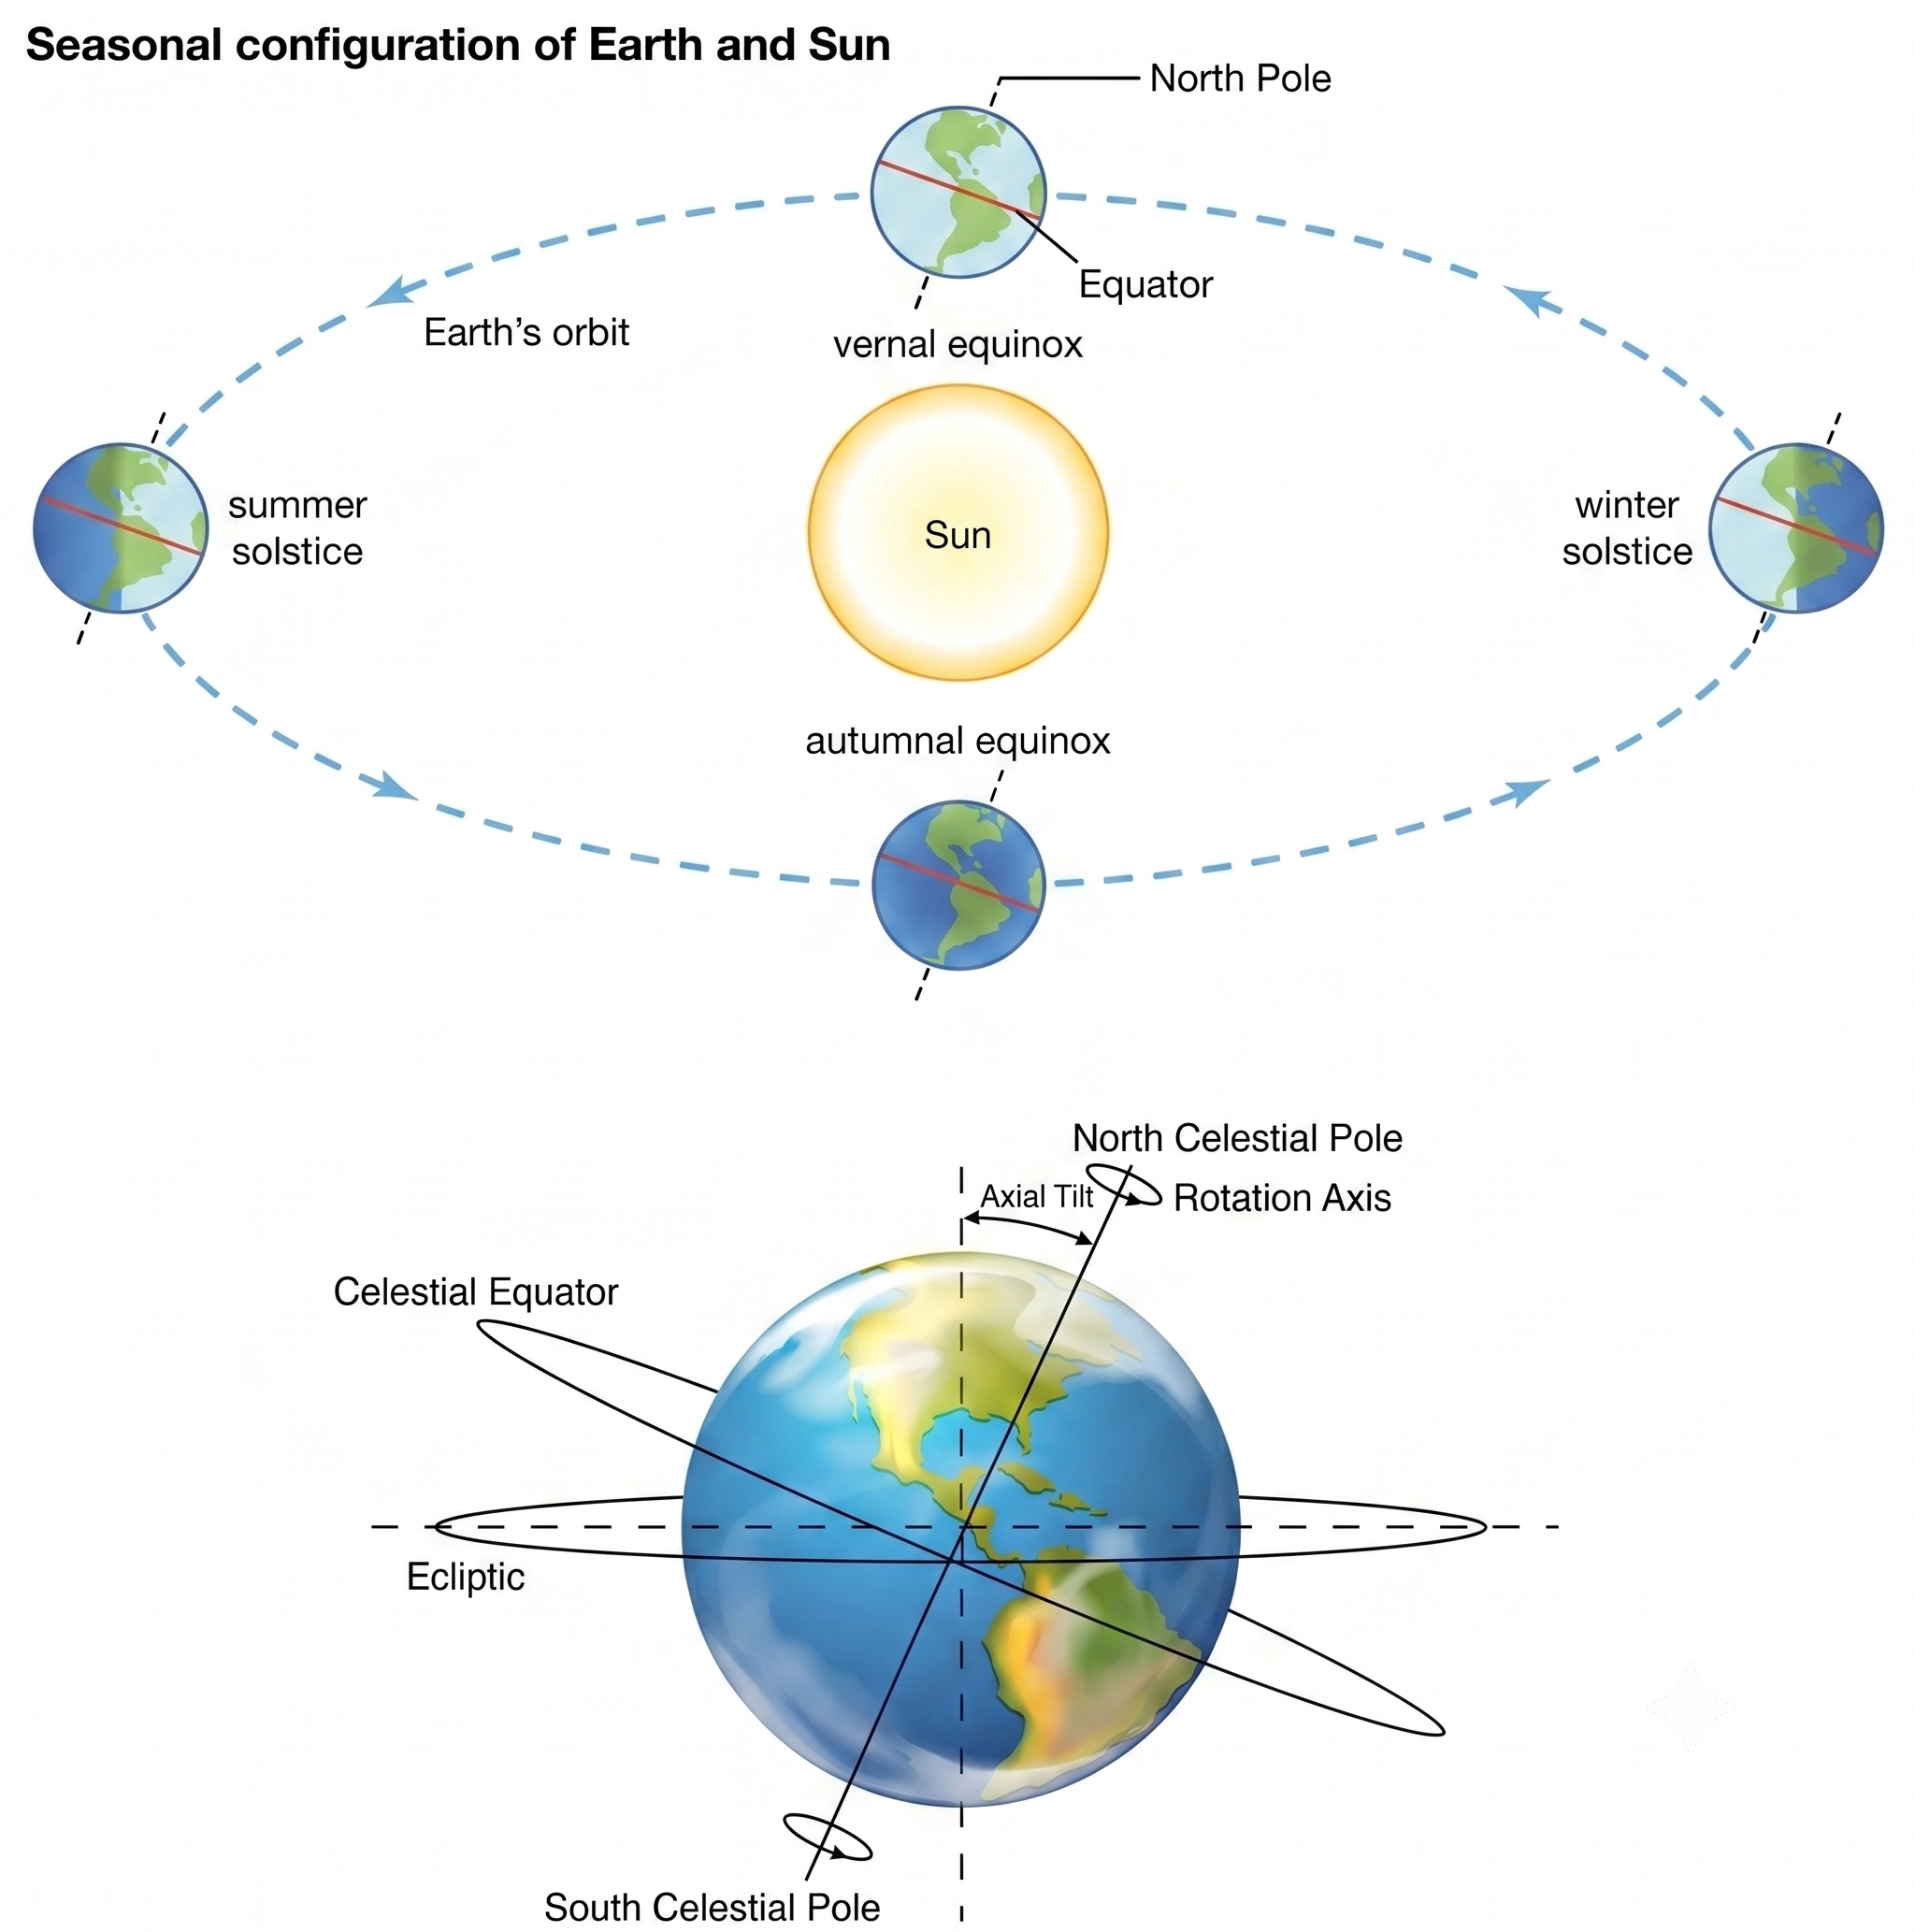
\includegraphics[width=\linewidth]{VERNAL_EQUINOX.png}
		\caption{The Sun crosses the celestial equator at the equinoxes ($\delta_\odot = 0^\circ$) and reaches extrema at the solstices ($\delta_\odot = \pm 23.44^\circ$).}
		\label{fig:vernal_equinox_fig}
	\end{minipage}
	\hfill
	\begin{minipage}[t]{0.48\textwidth}
		\centering
		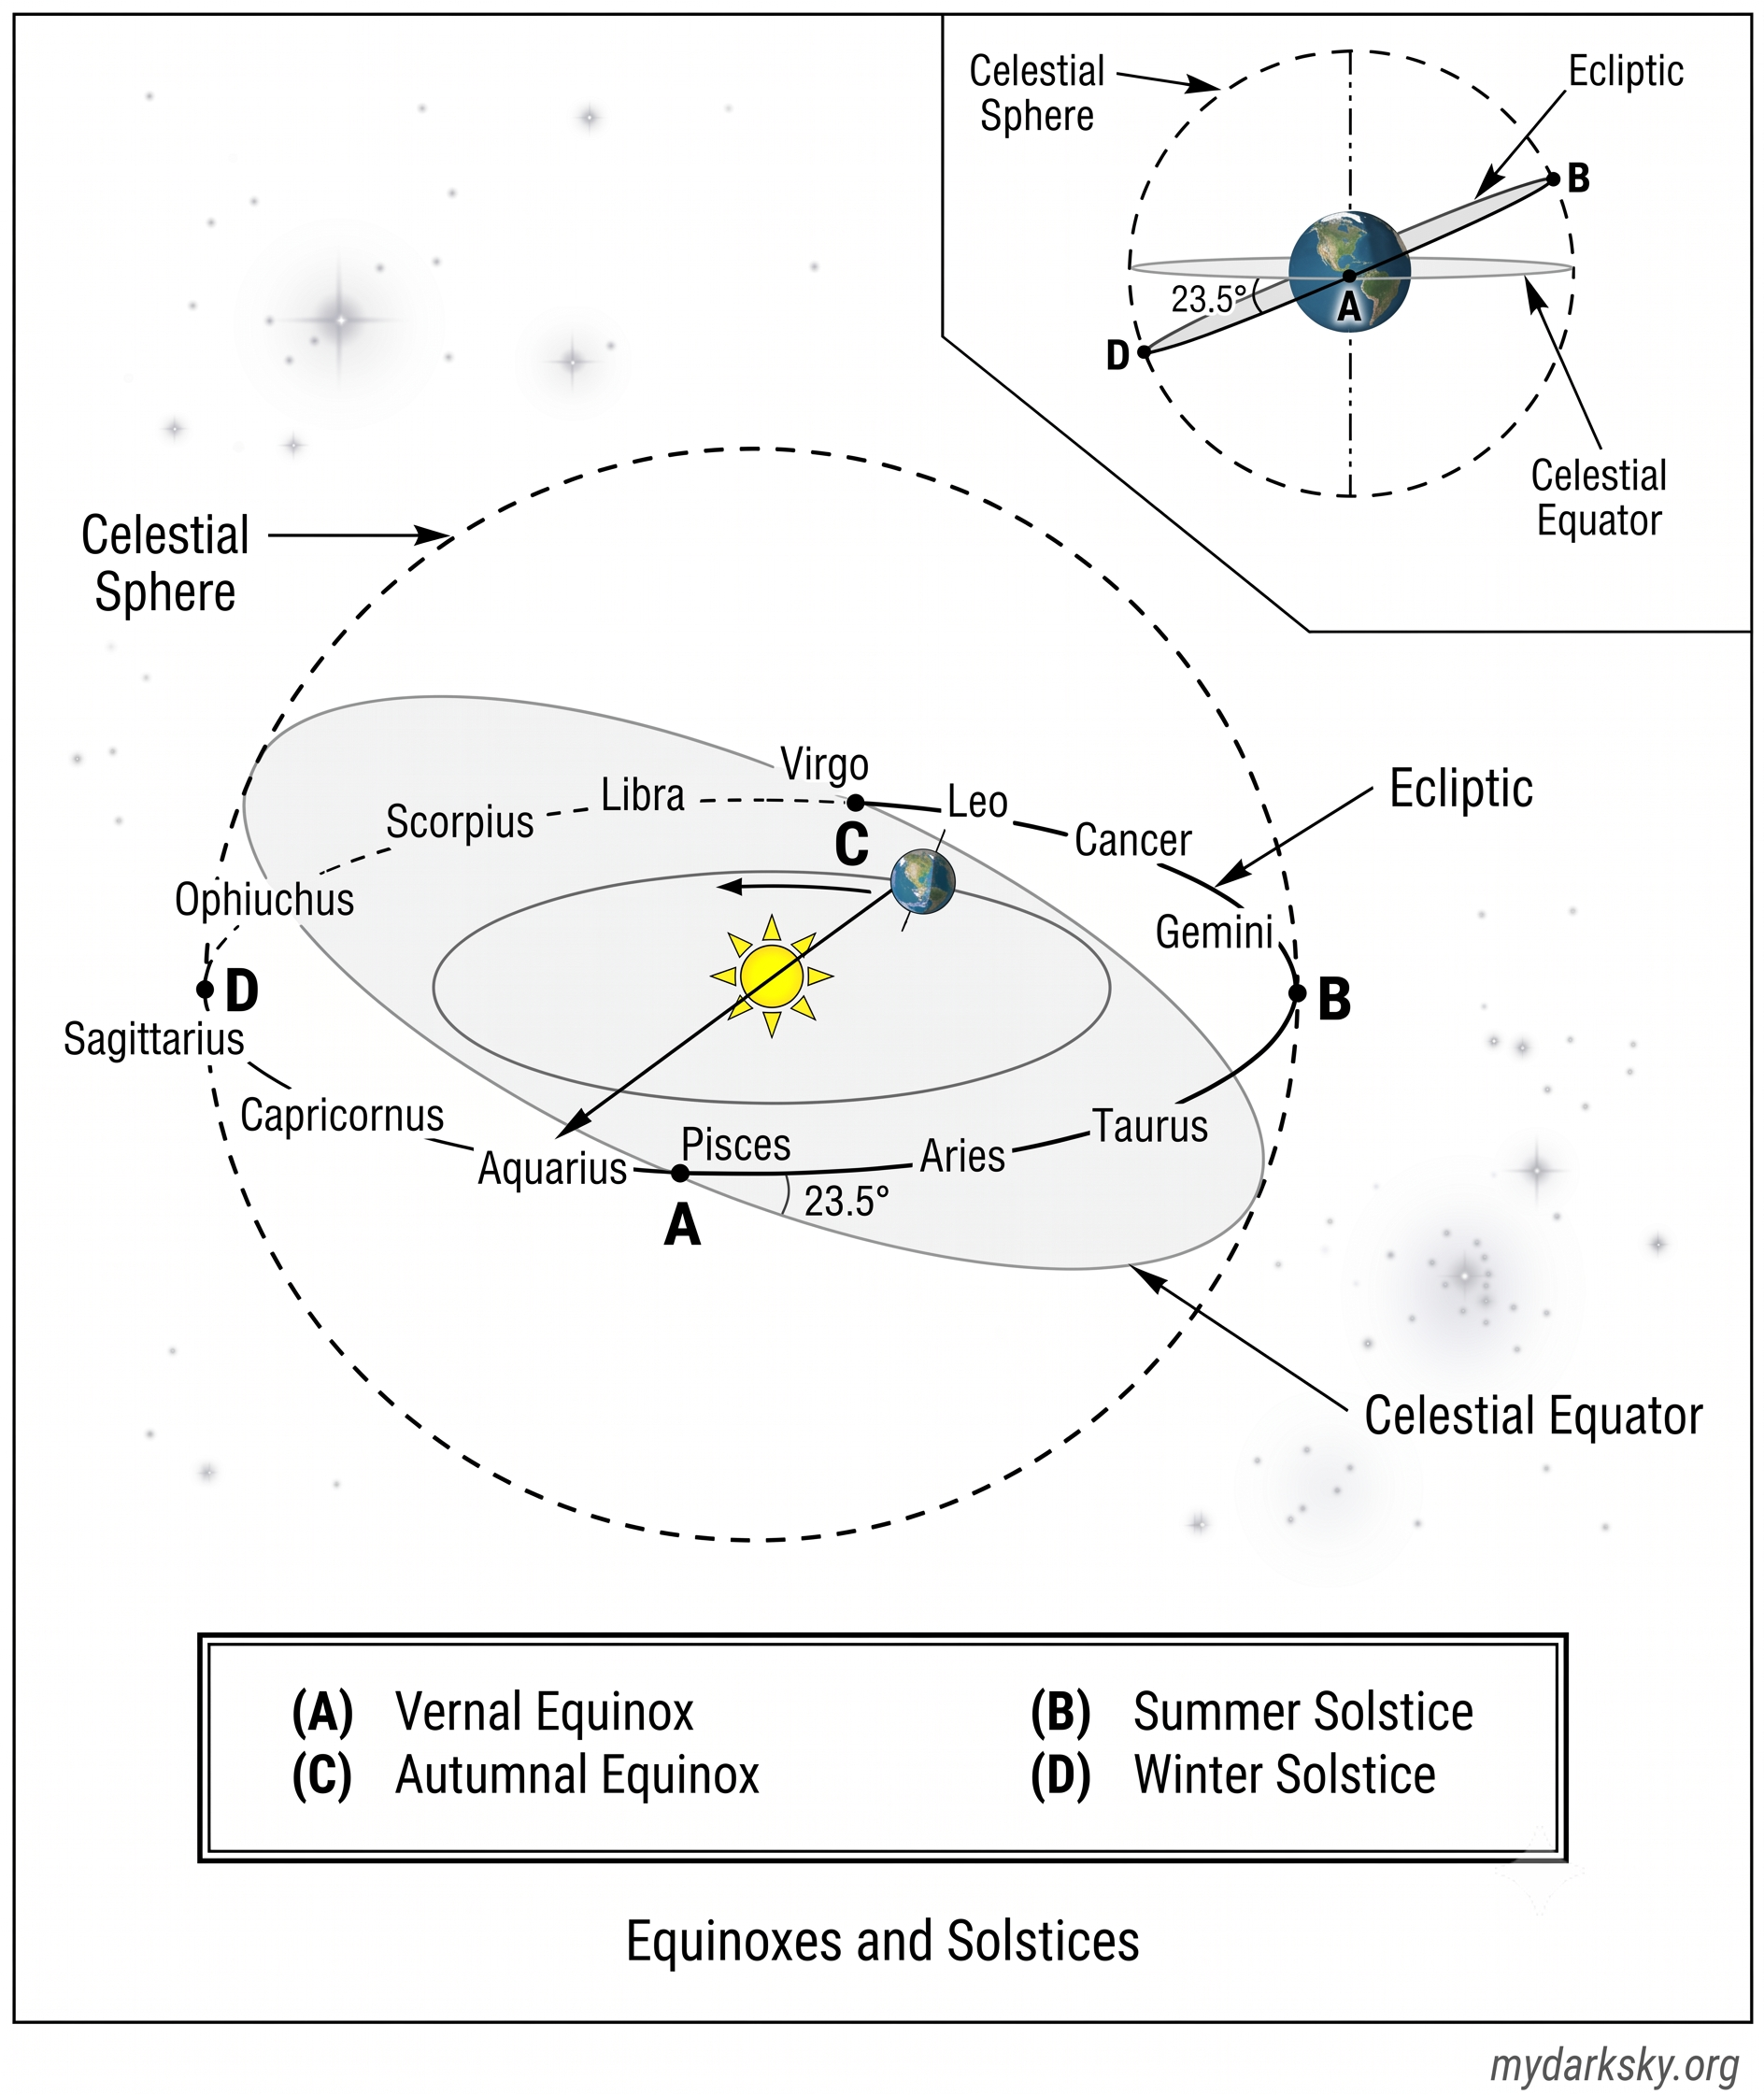
\includegraphics[width=\linewidth]{equinox_solstice_sm.png}
		\caption{Apparent path of the Sun along the ecliptic and the four cardinal seasonal milestones.}
		\label{fig:equinox_solstice_fig}
	\end{minipage}
\end{figure}

The Sun's equatorial coordinates and the corresponding Greenwich Sidereal Time at Greenwich solar noon ($\alpha_{\rm GM}$) at the cardinal seasonal milestones are:
\begin{align}
	\text{March (Vernal) Equinox (approx. Mar 21):}\quad &\alpha_\odot = 0^{\rm h}, &&\delta_\odot = 0^\circ, &&\alpha_{\rm GM} = 0^{\rm h}, \\
	\text{June (Summer) Solstice (approx. Jun 21):}\quad &\alpha_\odot = 6^{\rm h}, &&\delta_\odot \simeq +23.44^\circ, &&\alpha_{\rm GM} = 6^{\rm h}, \\
	\text{September (Autumnal) Equinox (approx. Sep 23):}\quad &\alpha_\odot = 12^{\rm h}, &&\delta_\odot = 0^\circ, &&\alpha_{\rm GM} = 12^{\rm h}, \\
	\text{December (Winter) Solstice (approx. Dec 21):}\quad &\alpha_\odot = 18^{\rm h}, &&\delta_\odot \simeq -23.44^\circ, &&\alpha_{\rm GM} = 18^{\rm h}.
\end{align}
At Greenwich local solar noon, the Sun is on the Greenwich meridian, so $\GST = \alpha_\odot$.

\section{The Equation of Time and the Solar Analemma}

A sundial measures \emph{Apparent Solar Time} ($\mathrm{AST}$), which tracks the hour angle of the physical Sun. However, apparent solar days are not of equal length throughout the year. Civil timekeeping is therefore based on \emph{Mean Solar Time} ($\mathrm{MST}$), which tracks a fictitious ``mean Sun'' that moves at a constant speed along the celestial equator.

\begin{definition}[Equation of Time]
	The \emph{Equation of Time} ($\EoT$) is defined as:
	\begin{keyresult}
		\begin{equation}
			\EoT \equiv \mathrm{AST} - \mathrm{MST} = \alpha_{\rm mean\,\odot} - \alpha_{\rm apparent\,\odot}.
			\label{eq:eot_def}
		\end{equation}
	\end{keyresult}
\end{definition}

The Equation of Time is the superposition of two independent physical phenomena:

\begin{enumerate}
	\item \textbf{Orbital Eccentricity Component ($e = 0.0167$):} In accordance with Kepler's Second Law, the Earth moves faster at perihelion (early January) and slower at aphelion (early July). The true Sun's apparent angular rate along the ecliptic varies as $\dot\lambda_\odot \propto 1/r^2$. This contributes an annual sinusoidal oscillation with an amplitude of $\approx 7.7\ \text{minutes}$:
	\begin{equation}
		\Delta t_e \approx -2e\sin M \approx -7.66\sin M\quad [\text{minutes}],
	\end{equation}
	where $M$ is the Earth's mean anomaly measured from perihelion.
	\item \textbf{Obliquity Component ($\epsilon = 23.44^\circ$):} Even if the Sun moved at a uniform angular speed along the ecliptic, projecting that motion onto the celestial equator introduces geometric non-uniformity:
	\begin{equation}
		\tan\alpha_\odot = \cos\epsilon\tan\lambda_\odot.
	\end{equation}
	Right ascension advances fastest at the solstices (where the ecliptic is parallel to the equator) and slowest at the equinoxes (where the ecliptic is inclined by $23.44^\circ$). This contributes a semi-annual harmonic with an amplitude of $\approx 9.9\ \text{minutes}$:
	\begin{equation}
		\Delta t_\epsilon \approx \frac{\tan^2(\epsilon/2)}{2}\sin(2\lambda_\odot) \approx 9.86\sin(2\lambda_\odot)\quad [\text{minutes}].
	\end{equation}
\end{enumerate}

\begin{figure}[htbp]
	\centering
	\begin{tikzpicture}[scale=1.1, font=\sffamily]
		\draw[->, thick] (0,0) -- (12.5,0) node[right] {Month};
		\draw[->, thick] (0,-3.5) -- (0,4.0) node[above] {$\EoT$ (minutes)};
		\draw[dashed, gray!40] (0,0) grid[xstep=1, ystep=1] (12,3.5);
		\draw[dashed, gray!40] (0,0) grid[xstep=1, ystep=1] (12,-3.5);
		
		% Ticks
		\foreach \x/\m in {1/Jan, 2/Feb, 3/Mar, 4/Apr, 5/May, 6/Jun, 7/Jul, 8/Aug, 9/Sep, 10/Oct, 11/Nov, 12/Dec} {
			\draw (\x, 0.1) -- (\x, -0.1) node[below=3pt, font=\footnotesize] {\m};
		}
		\foreach \y in {-15, -10, -5, 5, 10, 15} {
			\draw (0.1, \y*0.2) -- (-0.1, \y*0.2) node[left=3pt, font=\footnotesize] {\y};
		}
		
		% Component curves
		\draw[blue!70!black, thick, dashed, domain=0:12, samples=100] 
			plot (\x, {-7.66*sin(360*(\x-0.1)/12)*0.2});
		\node[blue!70!black, font=\footnotesize, right] at (1.5, -1.8) {Eccentricity ($e$)};
		
		\draw[red!70!black, thick, dotted, domain=0:12, samples=100] 
			plot (\x, {9.86*sin(720*(\x-2.7)/12)*0.2});
		\node[red!70!black, font=\footnotesize, right] at (7.2, 2.2) {Obliquity ($\epsilon$)};
		
		% Total curve
		\draw[black, ultra thick, domain=0:12, samples=200] 
			plot (\x, {(-7.66*sin(360*(\x-0.1)/12) + 9.86*sin(720*(\x-2.7)/12))*0.2});
		\node[black, font=\bfseries\footnotesize, right] at (9.8, 3.2) {Total $\EoT$};
	\end{tikzpicture}
	\caption{The Equation of Time decomposed into its two constituent physical components: orbital eccentricity ($e$, annual period) and obliquity ($\epsilon$, semi-annual period).}
	\label{fig:eot_decomposition}
\end{figure}

The total Equation of Time ranges between $-14.2\ \text{minutes}$ (in mid-February) and $+16.4\ \text{minutes}$ (in early November). Plotting the Sun's declination $\delta_\odot$ against the Equation of Time produces the famous figure-8 pattern known as the \emph{solar analemma}.

\section{Mean and Apparent Sidereal Time: The Equation of the Equinoxes}

Because the Earth is an oblate spheroid with an equatorial bulge, the gravitational forces exerted by the Moon and the Sun create torques that cause the Earth's rotation axis to precess and nutate in inertial space.

\begin{definition}[Mean versus True Equinox]
	\begin{itemize}
		\item The \emph{mean equinox} is the equinox position affected by smooth secular precession only.
		\item The \emph{true (apparent) equinox} is the instantaneous position of the equinox, including both secular precession and short-period nutation oscillations.
	\end{itemize}
\end{definition}

Sidereal time referenced to the mean equinox is \emph{Greenwich Mean Sidereal Time} ($\GMST$); sidereal time referenced to the true equinox is \emph{Greenwich Apparent Sidereal Time} ($\GAST$). They differ by the \emph{equation of the equinoxes}:
\begin{keyresult}
	\begin{equation}
		\GAST - \GMST = \Delta\psi\cos\epsilon \equiv \text{eqeq},
		\label{eq:equation_of_equinoxes}
	\end{equation}
\end{keyresult}
where $\Delta\psi$ is the nutation in longitude (dominated by the $18.6$-year regression of lunar nodes) and $\epsilon$ is the true obliquity. Because $|\text{eqeq}| \le 1.2\ \text{seconds}$, $\GMST$ suffices for casual observations, while $\GAST$ is essential for sub-arcsecond astrometry.

\subsection{Algorithmic Computation of GMST}

According to IAU conventions, $\GMST$ at $0^{\rm h}$ UT1 is computed from the Julian centuries $T$ elapsed since standard epoch J2000.0 ($T = (\JD - 2451545.0)/36525$):
\begin{equation}
	\GMST(0^{\rm h}\UT1) = 6^{\rm h}41^{\rm m}50.54841^{\rm s} + 8640184.812866^{\rm s}\,T + 0.093104^{\rm s}\,T^2 - 6.2 \times 10^{-6\,\rm s}\,T^3.
	\label{eq:gmst_iau_formula}
\end{equation}
At any instant of universal time $t_{\rm UT}$ (in hours):
\begin{equation}
	\GMST(t_{\rm UT}) = \GMST(0^{\rm h}\UT1) + 1.00273790935 \times t_{\rm UT}.
	\label{eq:gmst_instant}
\end{equation}

\section{Precession of the Equinoxes and Reference Epochs}

\begin{definition}[Lunisolar Precession]
	\emph{Lunisolar precession} is the slow, steady conical rotation of the Earth's spin axis around the normal to the ecliptic plane, with period $P_{\rm prec} \approx 25{,}772\ \text{years}$ (the Platonic Year). The spin axis traces out a cone of half-angle equal to the obliquity ($\epsilon \approx 23.44^\circ$), driven by the gravitational torque that the Sun and Moon exert on the Earth's oblate equatorial bulge --- the same torque-on-a-spinning-top mechanism responsible for ordinary gyroscopic precession.
\end{definition}

The vernal equinox drifts westward along the ecliptic at the rate:
\begin{equation}
	\dot\lambda_{\rm prec} \simeq 50.29''/\text{year} \approx 1^\circ/71.6\ \text{years}.
	\label{eq:precession_rate}
\end{equation}
Because the equatorial grid $(\alpha, \delta)$ is pinned to the moving equinox $\hat\gamma$, cataloged positions must always specify a standard epoch. The current international standard is epoch \textbf{J2000.0} (January 1, 2000, 12:00:00 TT).

To precess coordinates $(\alpha_0, \delta_0)$ from J2000.0 to an epoch $t$ with $\Delta t = t - 2000.0$ years:
\begin{keyresult}
	\begin{align}
		\alpha(t) &\approx \alpha_0 + (m + n\sin\alpha_0\tan\delta_0)\,\Delta t, \label{eq:precess_alpha} \\
		\delta(t) &\approx \delta_0 + (n\cos\alpha_0)\,\Delta t, \label{eq:precess_delta}
	\end{align}
\end{keyresult}
where the J2000.0 precession constants are $m = 3.075\ \text{s/yr} = 46.12''/\text{yr}$ and $n = 1.336\ \text{s/yr} = 20.04''/\text{yr}$.

\section{Modern Astronomical Time Scales: UT1, TAI, UTC, TT, and TDB}

Modern astrophysics requires a hierarchy of specialized time scales:

\begin{enumerate}
	\item \textbf{UT1 (Universal Time 1):} Measures the true rotation angle of the Earth about its axis, determined via VLBI observations of extragalactic quasars. Due to atmospheric winds, tidal friction, and core-mantle coupling, UT1 is non-uniform.
	\item \textbf{TAI (International Atomic Time):} A uniform atomic time scale generated by a weighted ensemble of hundreds of caesium-133 primary atomic clocks worldwide, defining the SI second ($9{,}192{,}631{,}770$ periods of the ground-state hyperfine transition).
	\item \textbf{UTC (Coordinated Universal Time):} The civil time standard. UTC runs at the SI rate of TAI, but integer \emph{leap seconds} are inserted at the end of June or December to maintain $|\UTC - \UT1| < 0.9\ \text{seconds}$:
	\begin{equation}
		\TAI - \UTC = \Delta\mathrm{AT} \quad (\text{currently } 37\ \text{seconds}).
	\end{equation}
	\item \textbf{TT (Terrestrial Time):} The theoretical coordinate time scale for clocks on the rotating geoid, free from Earth rotation irregularities:
	\begin{equation}
		\TT = \TAI + 32.184\ \text{s} \quad\Longrightarrow\quad \TT - \UTC = \Delta\mathrm{AT} + 32.184\ \text{s} \approx 69.184\ \text{s}.
	\end{equation}
	\item \textbf{TDB (Barycentric Dynamical Time):} The relativistic coordinate time scale evaluated at the Solar System Barycenter (SSB). It accounts for general relativistic gravitational redshift and orbital time dilation:
	\begin{equation}
		\TDB \approx \TT + 0.001657\sin(E + 0.01671\sin E)\ \text{s},
	\end{equation}
	where $E$ is the Earth's orbital eccentric anomaly. TDB is essential for pulsar timing arrays and interplanetary navigation.
\end{enumerate}

\section{Julian Date (JD) and Modified Julian Date (MJD)}

To track time continuously across millennia without calendar discontinuities, astronomers use the Julian Date system.

\begin{definition}[Julian Date]
	The \emph{Julian Date} ($\JD$) is the continuous count of days elapsed since Greenwich mean noon (12:00:00 UT) on January 1, 4713 BCE.
\end{definition}

\begin{definition}[Modified Julian Date]
	The \emph{Modified Julian Date} ($\MJD$) shifts the origin to Greenwich midnight and subtracts a large constant:
	\begin{keyresult}
		\begin{equation}
			\MJD \equiv \JD - 2{,}400{,}000.5.
			\label{eq:mjd_def}
		\end{equation}
	\end{keyresult}
	$\MJD = 0.0$ corresponds to midnight on November 17, 1858.
\end{definition}

\paragraph{Standard Astronomical Epochs:}
\begin{itemize}
	\item \textbf{Epoch J2000.0:} $\JD = 2{,}451{,}545.0$ (2000 Jan 1, 12:00:00 TT).
	\item \textbf{Epoch B1950.0:} $\JD = 2{,}433{,}282.423$.
\end{itemize}

\paragraph{Calendar Conversion Algorithm (Meeus 1998):}
For year $Y$, month $M$ ($1 \le M \le 12$), and decimal day $D$ (with UT fraction):
If $M = 1$ or $2$, set $Y \leftarrow Y - 1$ and $M \leftarrow M + 12$.
The Julian Date is computed via:
\begin{equation}
	A = \lfloor Y/100\rfloor, \qquad B = 2 - A + \lfloor A/4\rfloor,
\end{equation}
\begin{keyresult}
	\begin{equation}
		\JD = \lfloor 365.25(Y + 4716)\rfloor + \lfloor 30.6001(M + 1)\rfloor + D + B - 1524.5.
		\label{eq:jd_formula_meeus}
	\end{equation}
\end{keyresult}

With a continuous, unambiguous time coordinate now established, Chapter~2 turns to the companion problem of \emph{position}: fixing a coordinate grid on the celestial sphere itself. That grid is not static --- its very definition (the equatorial plane and the vernal equinox $\hat\gamma$) is tied to the precessing Earth axis derived above, which is why every catalogued equatorial coordinate must carry an epoch (Section~\ref{sec:coordinate_epochs}).

\chapter{Coordinate Systems on the Celestial Sphere}

Chapter~1 established the temporal frameworks -- solar time, sidereal time, and precession -- against which every astronomical observation must be referenced. To specify the locations of stars, planets, and galaxies, astronomers project the three-dimensional Universe onto the two-dimensional surface of an imaginary sphere of arbitrary radius centered on the observer: the \emph{celestial sphere}. Because astronomical measurements are performed from different vantage points (from an observatory on Earth, from the moving Earth relative to the Sun, or across the Milky Way), several coordinate systems are employed. In this chapter, we derive the four principal celestial coordinate systems --- Equatorial, Horizontal, Ecliptic, and Galactic --- and establish the rigorous vector transformations relating them.

\section{The Equatorial Coordinate System}

The \emph{equatorial coordinate system} extends the Earth's terrestrial latitude-longitude grid onto the celestial sphere: the celestial equator is the projection of the Earth's equator, the north and south celestial poles ($\mathrm{NCP}, \mathrm{SCP}$) are the projections of the Earth's rotation axis, and coordinates are fixed relative to the distant stars.

\begin{definition}[Right Ascension and Declination]
	\emph{Declination} $\delta \in [-90^\circ, +90^\circ]$ is the angular distance north ($+$) or south ($-$) of the celestial equator. \emph{Right ascension} $\alpha \in [0^{\rm h}, 24^{\rm h})$ ($0^\circ \le \alpha < 360^\circ$) is the angle measured eastward along the celestial equator from the vernal equinox $\hat\gamma$.
\end{definition}

\begin{figure}[htbp]
	\centering
	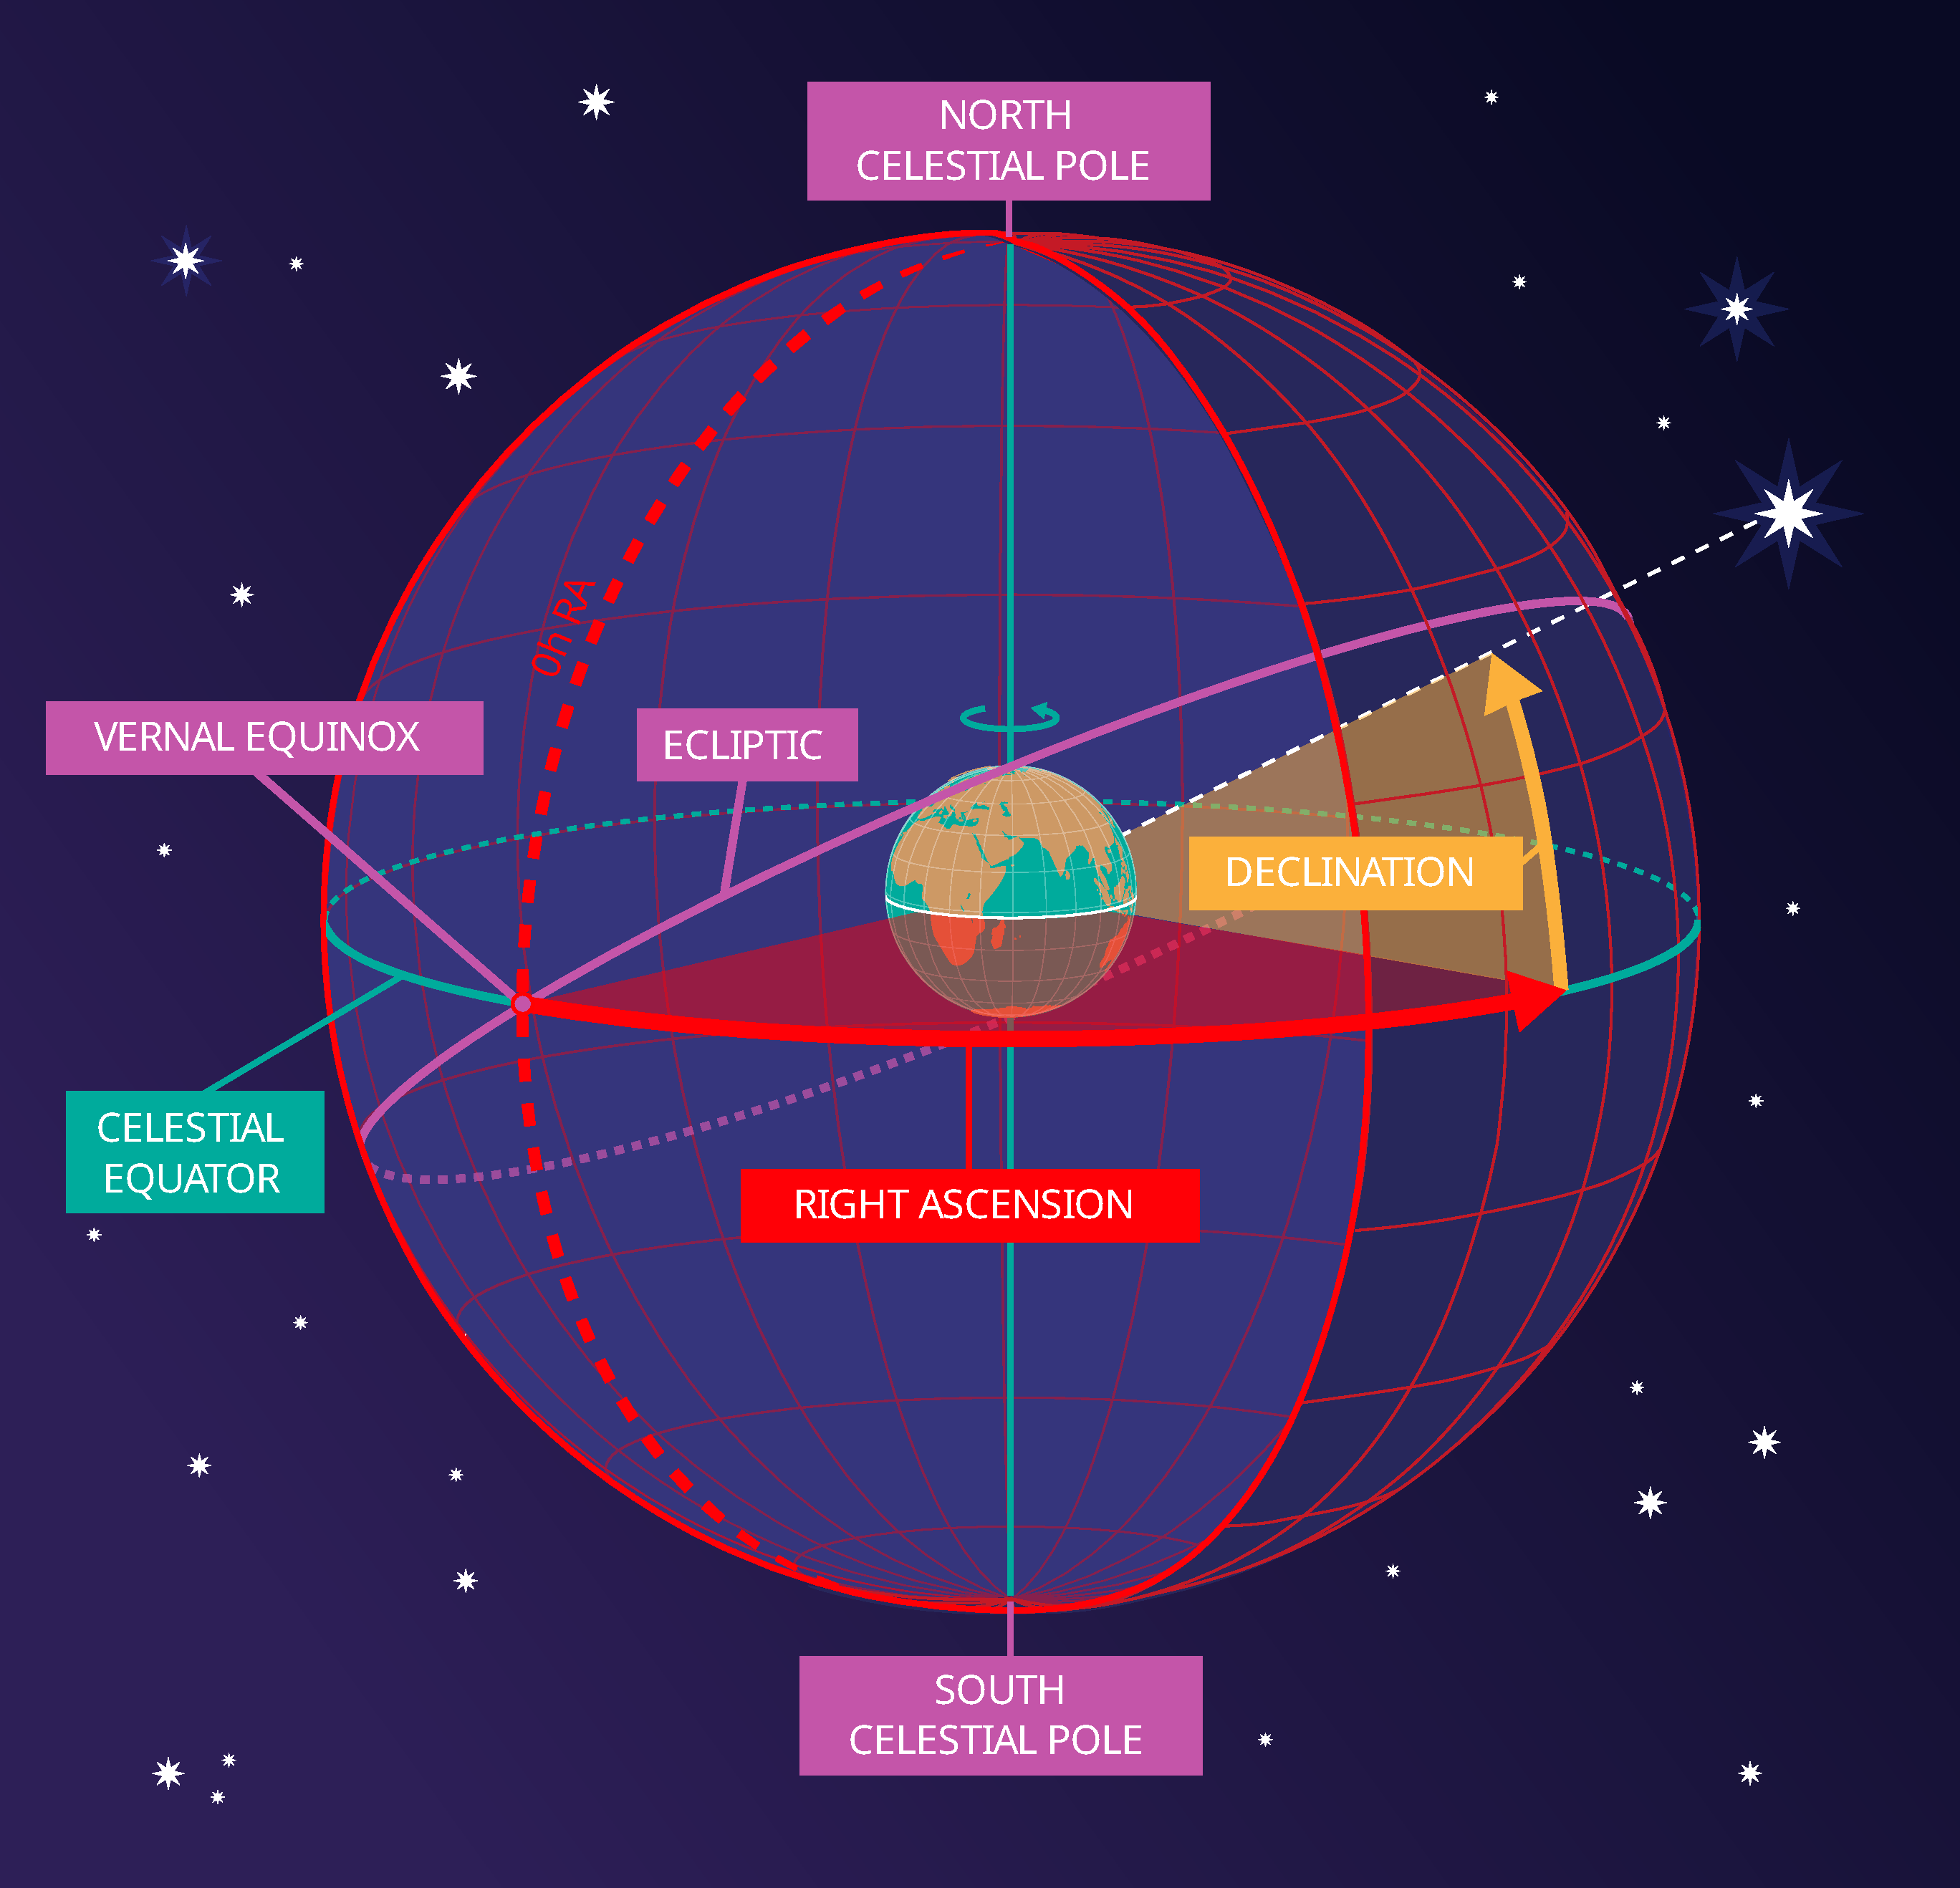
\includegraphics[width=0.55\linewidth]{declination_celestial_coordinates_en_bviPcZn.pdf}
	\caption{The equatorial Cartesian frame: the $z$-axis lies along the Earth's rotation axis ($\mathrm{NCP}$), the $xy$-plane is the celestial equator, and the $x$-axis points toward the vernal equinox $\hat\gamma$.}
	\label{fig:declination}
\end{figure}

In the equatorial Cartesian frame centered on the Earth, a source with coordinates $(\alpha, \delta)$ has the unit position vector:
\begin{keyresult}
	\begin{equation}
		\hat{\mathbf r}_{\rm eq} = \begin{pmatrix} \cos\delta\cos\alpha \\ \cos\delta\sin\alpha \\ \sin\delta \end{pmatrix}.
		\label{eq:unit_vector_eq}
	\end{equation}
\end{keyresult}

Because the equatorial grid is attached to the celestial sphere, stellar catalog coordinates $(\alpha, \delta)$ remain nearly constant on human timescales (subject only to proper motion and precession). The apparent daily rising and setting of celestial objects reflects the rotation of the observer's horizon underneath this fixed background.

\subsection{Coordinate Epochs}
\label{sec:coordinate_epochs}

Because the equinox $\hat\gamma$ that anchors the $(\alpha,\delta)$ grid precesses at the rate derived in Chapter~1 (Eq.~\eqref{eq:precession_rate}), a catalogued position $(\alpha,\delta)$ is meaningless without a stated \emph{epoch} -- the instant at which the equatorial grid used to define it is evaluated. The current standard is J2000.0; older catalogs commonly used B1950.0. Some source names encode the epoch directly in the identifier itself: for example, the pulsar $\mathrm{PSR\ J1939{+}2134}$ is named for its J2000 coordinates $\alpha \approx 19^{\rm h}39^{\rm m}$, $\delta \approx +21^\circ34'$.

Converting a cataloged position from one epoch to another in general requires \emph{two} independent corrections: the purely geometric precession of the reference grid (Eqs.~\eqref{eq:precess_alpha}--\eqref{eq:precess_delta}), and the star's own physical proper motion $(\mu_\alpha^*, \mu_\delta)$ across the sky (derived in Chapter~3). The two effects are independent and additive over the (typically short, $\Delta t \lesssim$ decades) baseline of a proper-motion correction, but only precession is required to transform a fixed grid definition (e.g.\ B1950.0 $\to$ J2000.0) when the object itself is treated as stationary.

\section{The Horizontal (Alt-Az) Coordinate System and the Hour Angle}

The \emph{horizontal} coordinate system is attached to the observer's local horizon and zenith, co-rotating with the Earth.

\begin{definition}[Altitude, Azimuth, and Hour Angle]
	\emph{Altitude} $h \in [-90^\circ, +90^\circ]$ is the angle of a celestial object above the local horizon (zenith at $h = 90^\circ$, nadir at $h = -90^\circ$). \emph{Azimuth} $A \in [0^\circ, 360^\circ)$ is the angle along the horizon measured from North ($0^\circ$) through East ($90^\circ$), South ($180^\circ$), and West ($270^\circ$). The \emph{Hour Angle} $H$ is the angular distance measured along the celestial equator from the local meridian to the object's hour circle:
	\begin{equation}
		H \equiv \LST - \alpha,
		\label{eq:hour_angle_formula}
	\end{equation}
	with $H > 0$ after meridian transit (moving westward).
\end{definition}

\begin{figure}[htbp]
	\centering
	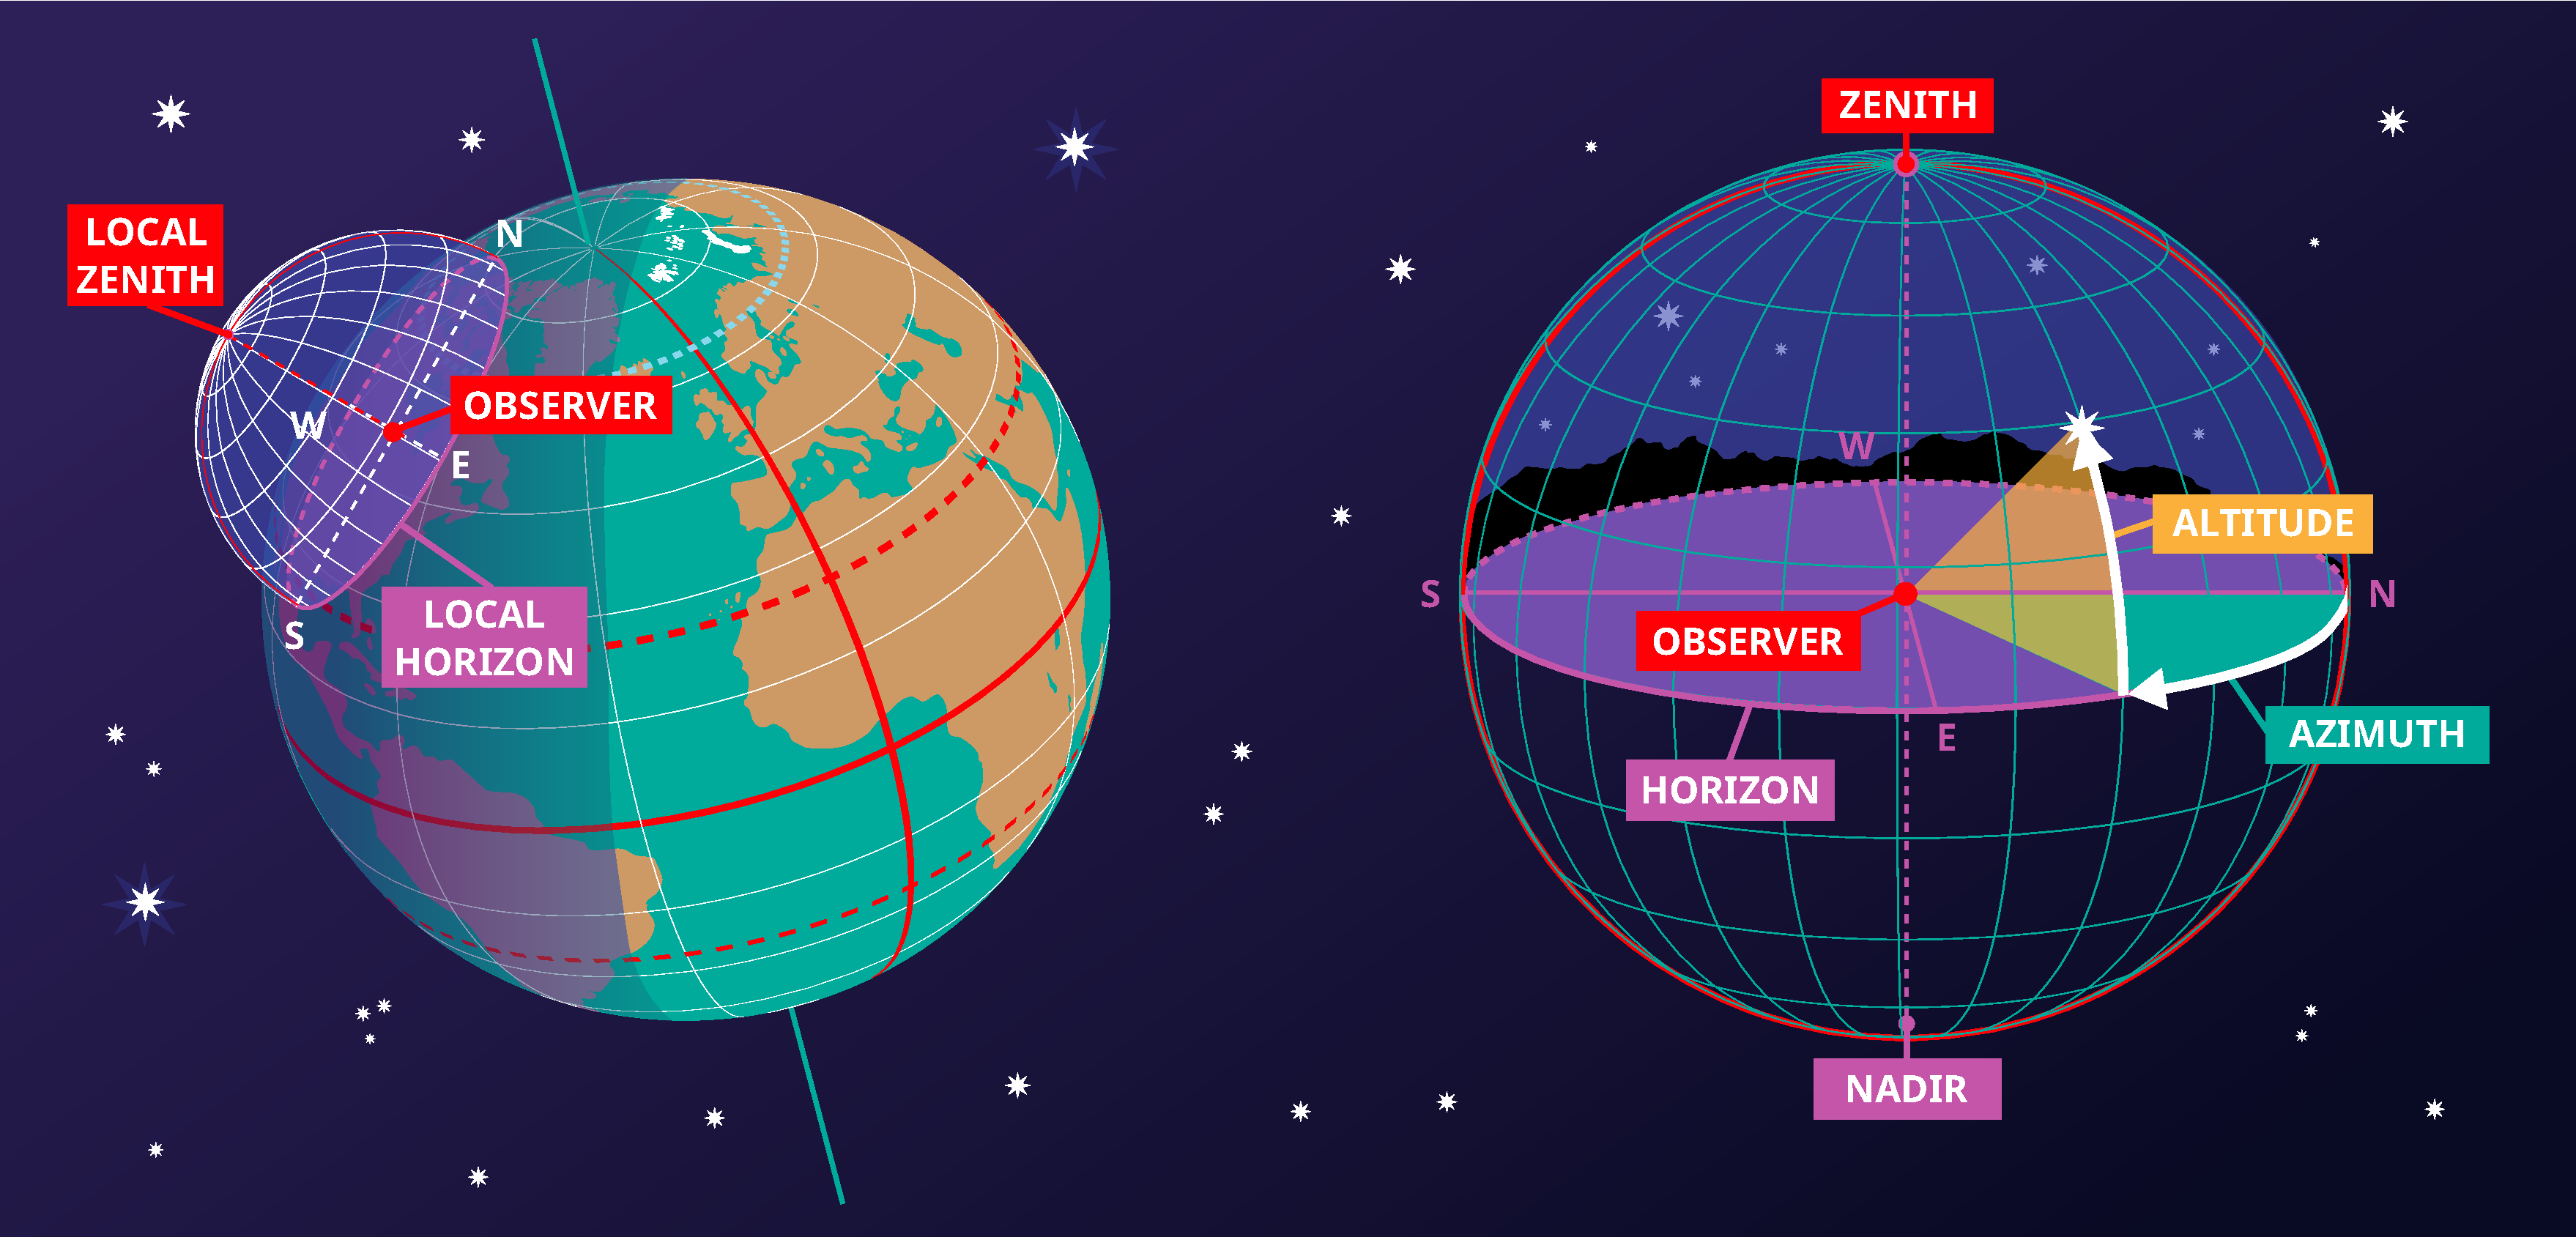
\includegraphics[width=0.75\linewidth]{altitude_azimuth_en.pdf}
	\caption{The horizontal coordinate system: the local meridian is the great circle passing through the North cardinal point, the Zenith, and the South cardinal point.}
	\label{fig:altaz}
\end{figure}

\section{Derivation of the Horizontal $\leftrightarrow$ Equatorial Transformations}

We now derive the transformations relating horizontal coordinates $(h, A)$ and equatorial coordinates $(\delta, H)$ for an observer at terrestrial latitude $\phi_0$. We express the unit vector toward a celestial source in two orthonormal coordinate frames sharing the same origin and relate them via an orthogonal rotation matrix.

\subsection{Source Vector in the Meridian-Aligned Equatorial Frame}

Align the Cartesian $x$-axis with the observer's \emph{local celestial meridian} at the instant of observation ($H = 0$). In this frame, the source's equatorial coordinate along the equator is $-H$:
\begin{equation}
	\hat{\mathbf s}_{\rm eq} = \begin{pmatrix} \cos\delta\cos(-H) \\ \cos\delta\sin(-H) \\ \sin\delta \end{pmatrix} = \begin{pmatrix} \cos\delta\cos H \\ -\cos\delta\sin H \\ \sin\delta \end{pmatrix}.
	\label{eq:unit_meridian_frame}
\end{equation}

\subsection{The Local Horizontal Basis}

The cardinal horizontal directions --- North ($\hat{\mathbf n}$), East ($\hat{\mathbf e}$), and Zenith ($\hat{\mathbf z}$) --- expressed in the meridian equatorial frame for latitude $\phi_0$ are:
\begin{itemize}
	\item \textbf{East ($\hat{\mathbf e}$):} Along the celestial equator, $90^\circ$ east of meridian: $(\delta, H) = (0, -90^\circ)$.
	\item \textbf{Zenith ($\hat{\mathbf z}$):} Overhead on the meridian: $(\delta, H) = (\phi_0, 0^\circ)$.
	\item \textbf{North ($\hat{\mathbf n}$):} Point on the horizon directly North, $90^\circ$ from zenith along the meridian: $(\delta, H) = (90^\circ + \phi_0, 0^\circ)$.
\end{itemize}

\begin{figure}[htbp]
	\begin{minipage}[b]{0.48\textwidth}
		\centering
		Substituting into Eq.~\eqref{eq:unit_meridian_frame}:
		\begin{align}
			\hat{\mathbf n} &= \begin{pmatrix} -\sin\phi_0 \\ 0 \\ \cos\phi_0 \end{pmatrix}, \label{eq:basis_n} \\
			\hat{\mathbf e} &= \begin{pmatrix} 0 \\ 1 \\ 0 \end{pmatrix}, \label{eq:basis_e} \\
			\hat{\mathbf z} &= \begin{pmatrix} \cos\phi_0 \\ 0 \\ \sin\phi_0 \end{pmatrix}. \label{eq:basis_z}
		\end{align}
	\end{minipage}
	\hfill
	\begin{minipage}[b]{0.48\textwidth}
		\centering
		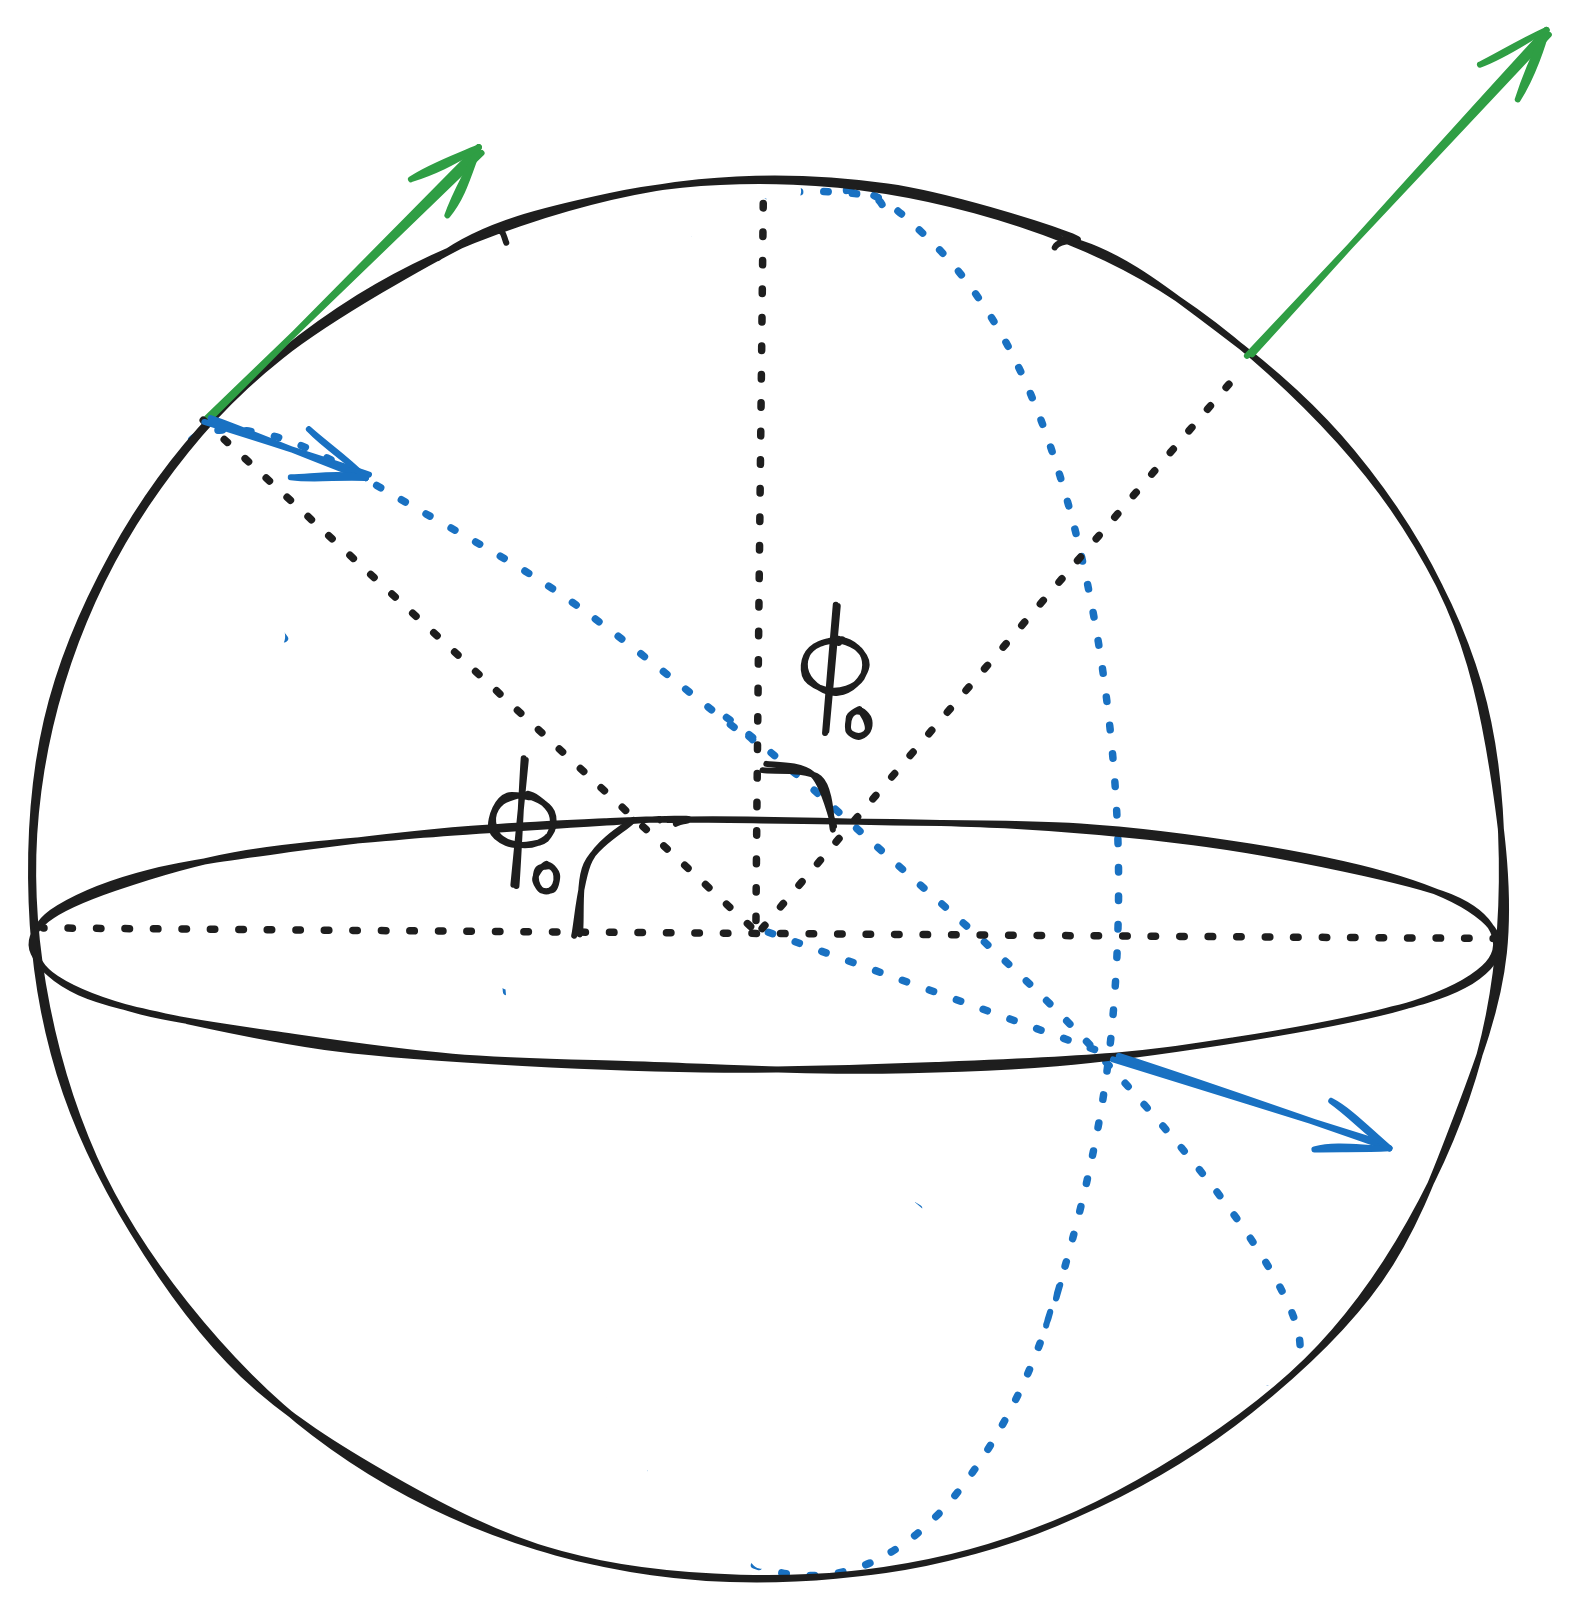
\includegraphics[width=0.7\linewidth]{local north and east.png}
		\caption{Local horizontal basis directions $\{\hat{\mathbf n}, \hat{\mathbf e}, \hat{\mathbf z}\}$.}
		\label{fig:local_coordinates}
	\end{minipage}
\end{figure}

\subsection{Transformation Equations}

Any unit vector can be decomposed in the horizontal basis $(h, A)$ as:
\begin{equation}
	\hat{\mathbf s} = (\cos h\cos A)\,\hat{\mathbf n} + (\cos h\sin A)\,\hat{\mathbf e} + (\sin h)\,\hat{\mathbf z}.
\end{equation}
Using the orthogonal rotation matrix $\mathbf R$:
\begin{equation}
	\begin{pmatrix} \cos h\cos A \\ \cos h\sin A \\ \sin h \end{pmatrix} = \begin{pmatrix} -\sin\phi_0 & 0 & \cos\phi_0 \\ 0 & 1 & 0 \\ \cos\phi_0 & 0 & \sin\phi_0 \end{pmatrix} \begin{pmatrix} \cos\delta\cos H \\ -\cos\delta\sin H \\ \sin\delta \end{pmatrix}.
	\label{eq:eq_to_hor_matrix}
\end{equation}
Multiplying out row by row yields the fundamental transformation relations:
\begin{keyresult}
	\begin{align}
		\sin h &= \sin\phi_0\sin\delta + \cos\phi_0\cos\delta\cos H, \label{eq:sinh_master} \\
		\cos h\sin A &= -\cos\delta\sin H, \label{eq:cosh_sinA} \\
		\cos h\cos A &= -\sin\phi_0\cos\delta\cos H + \cos\phi_0\sin\delta. \label{eq:cosh_cosA}
	\end{align}
\end{keyresult}
Dividing Eq.~\eqref{eq:cosh_sinA} by Eq.~\eqref{eq:cosh_cosA} gives the azimuth:
\begin{equation}
	\tan A = \frac{-\cos\delta\sin H}{-\sin\phi_0\cos\delta\cos H + \cos\phi_0\sin\delta} = \frac{\sin H}{\sin\phi_0\cos H - \cos\phi_0\tan\delta}.
	\label{eq:tanA_master}
\end{equation}

\begin{example}[Sirius at LST $22^{\rm h}00^{\rm m}$ from IISER TVM]
	For Sirius ($\alpha = 06^{\rm h}45^{\rm m}09^{\rm s}$, $\delta = -16.716^\circ$) observed from IISER TVM ($\phi_0 = 8.6833^\circ\text{N}$) at $\LST = 22^{\rm h}00^{\rm m}00^{\rm s}$:
	\[
	H = \LST - \alpha = 15^{\rm h}14^{\rm m}51^{\rm s} \approx 228.71^\circ.
	\]
	From Eq.~\eqref{eq:sinh_master}:
	\[
	\sin h = \sin(8.6833^\circ)\sin(-16.716^\circ) + \cos(8.6833^\circ)\cos(-16.716^\circ)\cos(228.71^\circ) = -0.668 \implies h \approx -41.9^\circ.
	\]
	Sirius is well below the horizon. From Eq.~\eqref{eq:tanA_master}, taking into account signs of numerator and denominator, $A \approx 104.74^\circ$.
\end{example}

\section{Rising, Setting, and Circumpolar Stars}

A celestial object rises or sets when its geometric center crosses the true horizon ($h = 0^\circ$). Setting $h = 0$ in Eq.~\eqref{eq:sinh_master}:
\begin{keyresult}
	\begin{equation}
		\cos H_0 = -\tan\phi_0\tan\delta.
		\label{eq:rise_set_master}
	\end{equation}
\end{keyresult}
This yields two solutions:
\begin{itemize}
	\item \textbf{Setting:} $H = +H_0 = \arccos(-\tan\phi_0\tan\delta) > 0$.
	\item \textbf{Rising:} $H = -H_0 = -\arccos(-\tan\phi_0\tan\delta) < 0$.
\end{itemize}
The local sidereal times of rising and setting are $\LST_{\rm rise} = \alpha - H_0$ and $\LST_{\rm set} = \alpha + H_0$.

\begin{figure}[htbp]
	\centering
	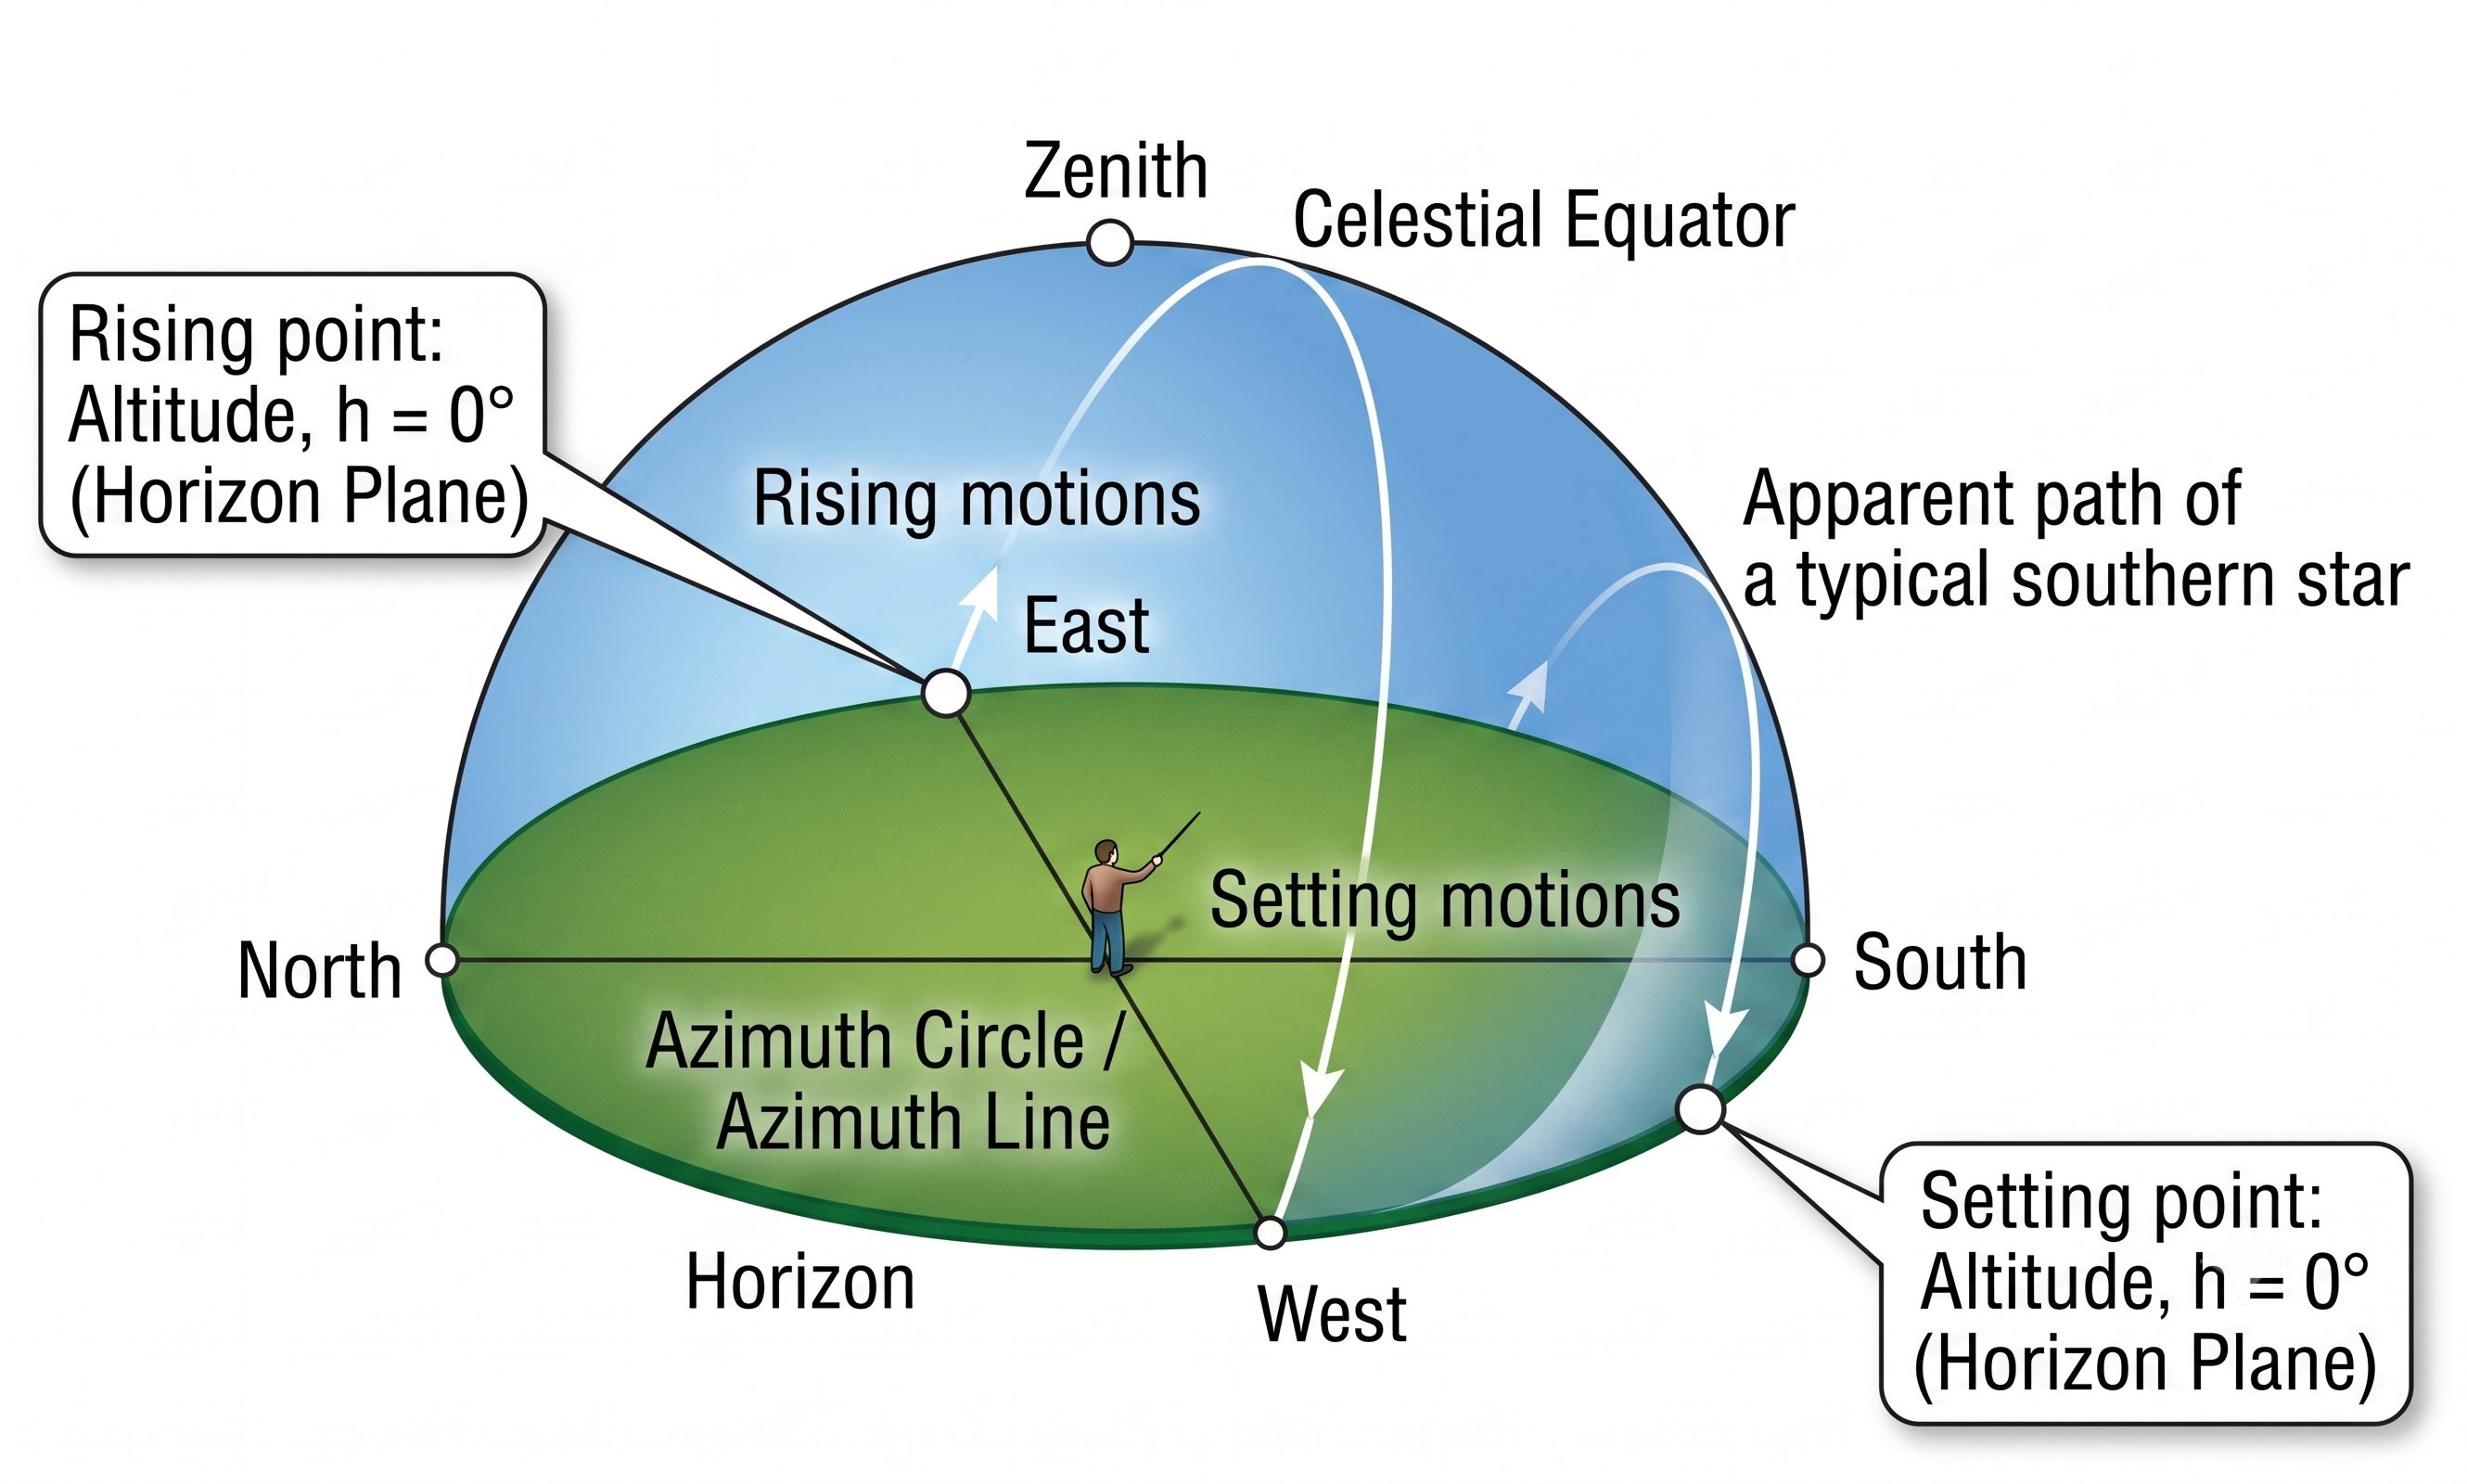
\includegraphics[width=0.55\linewidth]{rising-setting.png}
	\caption{Diurnal motion of stars along small circles of constant declination.}
	\label{fig:rising_setting}
\end{figure}

\paragraph{Circumpolar and Never-Rising Conditions.}
The quantity $|\tan\phi_0\tan\delta|$ determines visibility:
\begin{itemize}
	\item If $|\tan\phi_0\tan\delta| \le 1$: The star rises and sets daily.
	\item If $\tan\phi_0\tan\delta > 1$ ($\delta > 90^\circ - |\phi_0|$ in Northern hemisphere): The object is \emph{circumpolar} and never sets ($\cos H_0 < -1$, $h > 0$ always).
	\item If $\tan\phi_0\tan\delta < -1$ ($\delta < -(90^\circ - |\phi_0|)$): The object \emph{never rises} above the horizon.
\end{itemize}

\section{Zenith Angle at Meridian Transit and Local Solar Noon}

\begin{definition}[Zenith Angle]
	The \emph{zenith angle} $z$ is the angular distance from the observer's zenith:
	\begin{equation}
		z = 90^\circ - h.
		\label{eq:zenith_angle_def}
	\end{equation}
\end{definition}

At upper meridian transit (culmination), $H = 0$, so $\cos H = 1$. Eq.~\eqref{eq:sinh_master} simplifies to:
\[
\sin h_{\rm max} = \sin\phi_0\sin\delta + \cos\phi_0\cos\delta = \cos(\phi_0 - \delta).
\]
Since $\sin h = \cos z$, this yields the fundamental relation:
\begin{keyresult}
	\begin{equation}
		z_{\rm min} = |\phi_0 - \delta|.
		\label{eq:zenith_angle_noon}
	\end{equation}
\end{keyresult}
At local solar noon ($\delta = \delta_\odot$), the Sun's zenith angle is simply $z_{\rm noon} = |\phi_0 - \delta_\odot|$.

\begin{example}[Summer Solstice Noon at IISER TVM]
	At the June solstice, $\delta_\odot = +23.44^\circ$. For IISER TVM ($\phi_0 = 8.6833^\circ\text{N}$):
	\[
	z_{\rm noon} = |8.6833^\circ - 23.44^\circ| = 14.76^\circ.
	\]
	The Sun culminates $14.76^\circ$ north of zenith.
\end{example}

\section{Atmospheric Refraction and Stellar Aberration}

\subsection{Atmospheric Refraction}
As starlight enters the Earth's atmosphere, the increasing refractive index bends the ray toward the zenith, making objects appear \emph{higher} than their true geometric altitude:
\begin{equation}
	h_{\rm apparent} = h_{\rm true} + R(h).
\end{equation}
To see where the numerical coefficient in this bending comes from, again use the plane-parallel approximation: treat the atmosphere as a single slab of refractive index $n$ (vacuum, $n=1$, above it). Snell's law relates the true zenith angle $z$ (outside the atmosphere) to the apparent zenith angle $z' = z - R$ seen by the observer at the surface:
\begin{equation}
	\sin z = n\sin z' = n\sin(z - R).
\end{equation}
Expanding $\sin(z-R) \approx \sin z - R\cos z$ for small $R$:
\begin{equation}
	\sin z \approx n\sin z - nR\cos z \quad\Longrightarrow\quad R \approx \frac{(n-1)\sin z}{n\cos z} \approx (n-1)\tan z,
	\label{eq:refraction_derivation}
\end{equation}
using $n\approx 1$ in the denominator. With the refractive index of air at the surface $n - 1 \approx 2.8\times10^{-4}$ (a measured property of air, not something derivable from geometry alone), and converting to arcseconds ($1\,\text{rad} = 206{,}265''$):
\begin{keyresult}
	\begin{equation}
		R \approx (n-1)\tan z \times 206{,}265'' \approx 58.2''\tan z = 58.2''\cot h_{\rm true} \qquad (h_{\rm true} > 15^\circ).
		\label{eq:refraction_cot}
	\end{equation}
\end{keyresult}
Because $n-1$ itself depends on air density (hence on local temperature and pressure), this coefficient is only a standard-atmosphere reference value; the empirical formula below builds in an explicit correction for the actual $(P,T)$ at the telescope. Near the horizon, the single-slab approximation breaks down entirely (as $z\to90^\circ$ the ray grazes the atmosphere over a curved path), so Bennett's formula provides sub-arcsecond accuracy there instead, as an empirical fit rather than a derived result:
\begin{equation}
	R[\text{arcmin}] \approx \frac{1.02}{\tan\!\left(h + \dfrac{10.3^\circ}{h + 5.11^\circ}\right)}\times\left(\frac{P}{1010\,\text{hPa}}\right)\left(\frac{283}{273 + T[^\circ\text{C}]}\right).
	\label{eq:bennett_formula}
\end{equation}
At the horizon ($h = 0^\circ$), $R \approx 34'$ (greater than the Sun's angular diameter $\sim 32'$).

\subsection{Stellar Aberration}
The finite speed of light combined with the observer's own motion tilts the apparent direction of an incoming ray, exactly as vertically falling rain appears to slant forward when run through by a moving observer. Consider a photon arriving from directly overhead (velocity $-c\hat{\vec y}$ in the Sun's rest frame) while the Earth moves with velocity $v\hat{\vec x}$ transverse to that direction. Since $v \ll c$, Galilean velocity addition is an excellent approximation: in the Earth's frame, the photon's apparent velocity is
\begin{equation}
	\vec c\,' = \vec c - \vec v = -v\,\hat{\vec x} - c\,\hat{\vec y},
\end{equation}
so the ray appears tilted from the vertical by an angle $\kappa$ with
\begin{equation}
	\tan\kappa = \frac{v}{c} \quad\Longrightarrow\quad \kappa \approx \frac{v}{c} \quad (\text{since } v\ll c).
\end{equation}
Using Earth's orbital speed $v \approx 29.8\,\mathrm{km/s}$ (transverse to the line of sight to a star near the ecliptic pole, the maximal case) and converting to arcseconds:
\begin{keyresult}
	\begin{equation}
		\kappa = \frac{v}{c} \approx 20.4955'' \approx 20.5''.
		\label{eq:aberration_constant}
	\end{equation}
\end{keyresult}
Because $v$ is Earth's \emph{orbital} velocity, $\kappa$ varies sinusoidally over the year and traces out a small ellipse (or, for stars at the ecliptic pole, a circle) of angular semi-major axis $20.5''$ on the sky --- geometrically a much smaller, much faster analogue of the parallax ellipse of Chapter~3, and one that (unlike parallax) is completely independent of the star's distance.

\section{Angular Distance on a Sphere}

The angular separation $\theta$ between two points $(\alpha_1, \delta_1)$ and $(\alpha_2, \delta_2)$ is given by the dot product of their unit vectors (Eq.~\eqref{eq:unit_vector_eq}), since for any two unit vectors $\cos\theta = \hat{\mathbf r}_1\cdot\hat{\mathbf r}_2$:
\begin{align}
	\cos\theta &= (\cos\delta_1\cos\alpha_1)(\cos\delta_2\cos\alpha_2) + (\cos\delta_1\sin\alpha_1)(\cos\delta_2\sin\alpha_2) + \sin\delta_1\sin\delta_2 \notag \\
	&= \cos\delta_1\cos\delta_2\big(\cos\alpha_1\cos\alpha_2 + \sin\alpha_1\sin\alpha_2\big) + \sin\delta_1\sin\delta_2,
\end{align}
which, using $\cos\alpha_1\cos\alpha_2+\sin\alpha_1\sin\alpha_2=\cos(\alpha_1-\alpha_2)$, gives the spherical law of cosines:
\begin{keyresult}
	\begin{equation}
		\cos\theta = \hat{\mathbf r}_1 \cdot \hat{\mathbf r}_2 = \sin\delta_1\sin\delta_2 + \cos\delta_1\cos\delta_2\cos(\alpha_1 - \alpha_2).
		\label{eq:spherical_law_cos}
	\end{equation}
\end{keyresult}
For small angular separations ($\theta \ll 1$), the Haversine formula avoids floating-point precision loss:
\begin{equation}
	\sin^2\left(\frac{\theta}{2}\right) = \sin^2\left(\frac{\delta_2 - \delta_1}{2}\right) + \cos\delta_1\cos\delta_2\sin^2\left(\frac{\alpha_2 - \alpha_1}{2}\right).
	\label{eq:haversine_formula}
\end{equation}

\section{The Ecliptic Coordinate System}

\begin{definition}[Ecliptic Coordinates]
	\emph{Ecliptic longitude} $\lambda \in [0^\circ, 360^\circ)$ is measured eastward along the ecliptic from $\hat\gamma$. \emph{Ecliptic latitude} $\beta \in [-90^\circ, +90^\circ]$ is measured perpendicular to the ecliptic plane.
\end{definition}

\begin{figure}[htbp]
	\centering
	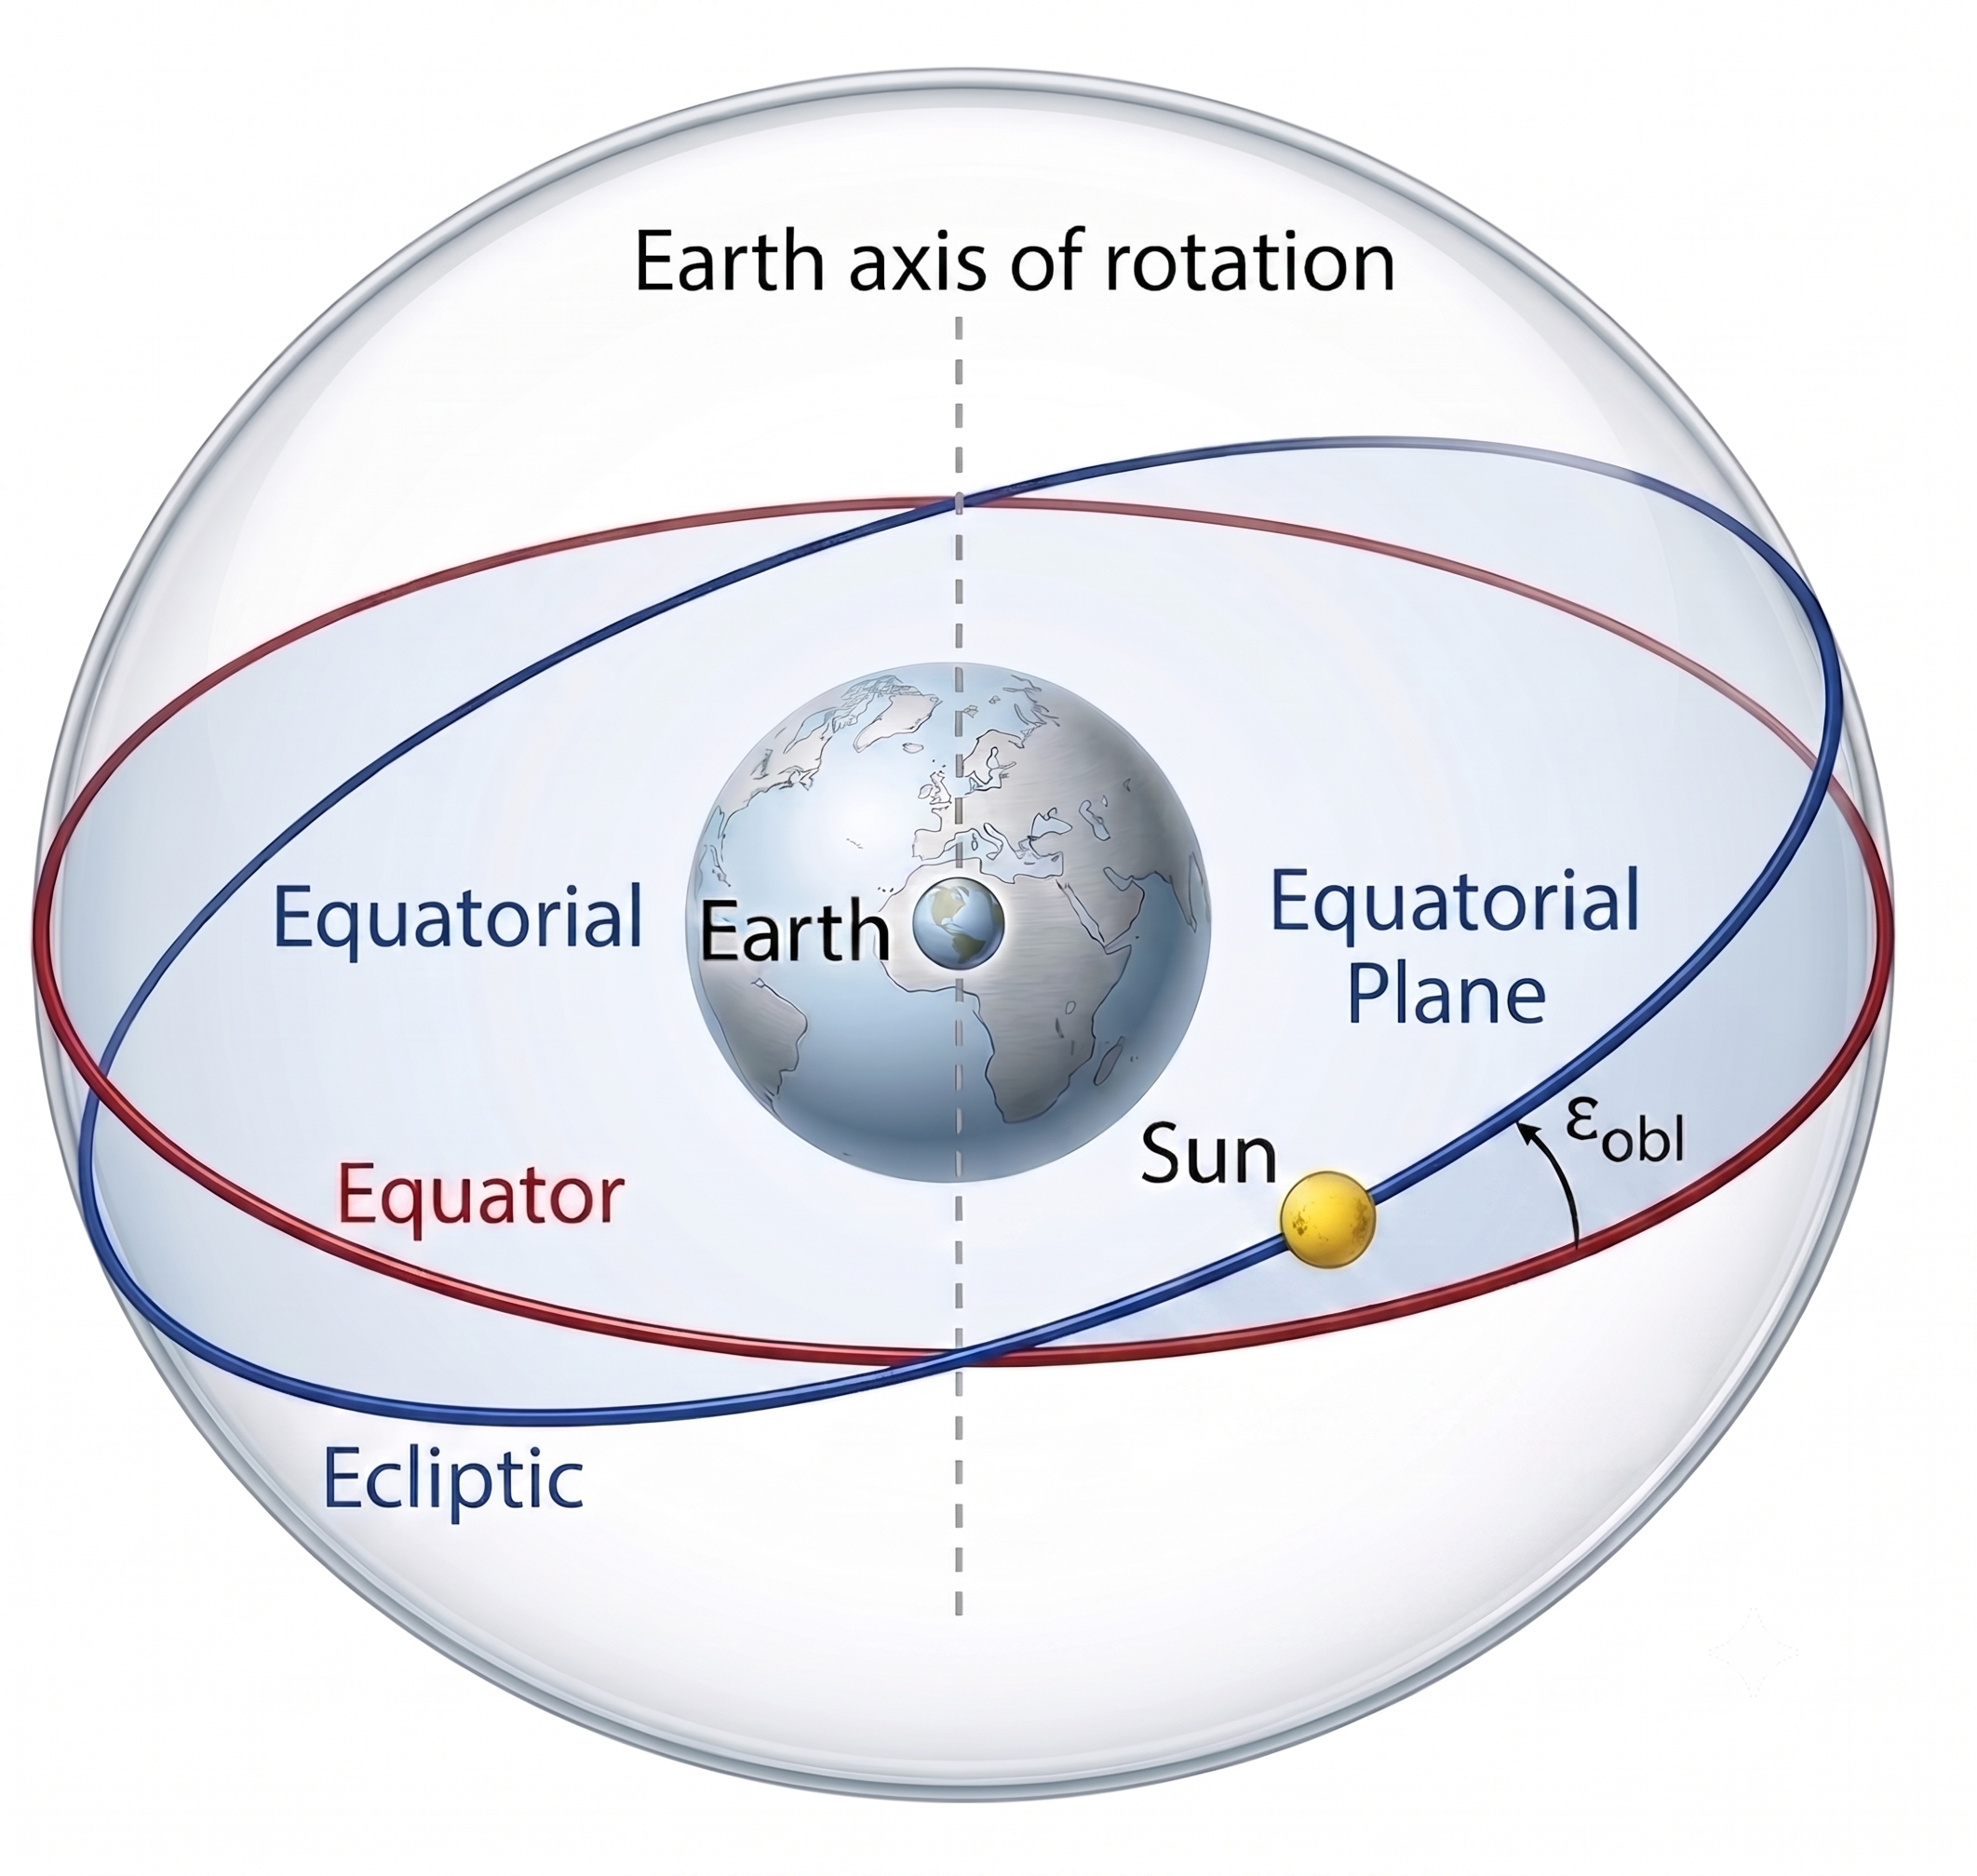
\includegraphics[width=0.4\linewidth]{Equator-Elliptic.png}
	\caption{Obliquity of the ecliptic $\epsilon \approx 23.44^\circ$ relating equatorial and ecliptic planes.}
	\label{fig:equator_elliptic}
\end{figure}

The ecliptic and equatorial planes intersect exactly along the line to the vernal equinox $\hat\gamma$ (by definition of $\hat\gamma$, Section~\ref{sec:sun_coordinates} of Chapter~1), so a rotation by the obliquity $\epsilon$ about that shared axis (the Cartesian $x$-axis in both frames) carries one frame into the other --- precisely the same kind of orthogonal-rotation-matrix argument used to derive the horizontal transformation above, only with a fixed rotation axis and angle rather than one set by the observer's latitude:
\begin{equation}
	\begin{pmatrix} \cos\beta\cos\lambda \\ \cos\beta\sin\lambda \\ \sin\beta \end{pmatrix} = \begin{pmatrix} 1 & 0 & 0 \\ 0 & \cos\epsilon & \sin\epsilon \\ 0 & -\sin\epsilon & \cos\epsilon \end{pmatrix} \begin{pmatrix} \cos\delta\cos\alpha \\ \cos\delta\sin\alpha \\ \sin\delta \end{pmatrix}.
	\label{eq:ecliptic_rotation_matrix}
\end{equation}
This yields:
\begin{keyresult}
	\begin{align}
		\sin\beta &= \sin\delta\cos\epsilon - \cos\delta\sin\alpha\sin\epsilon, \label{eq:ecliptic_beta} \\
		\cos\beta\cos\lambda &= \cos\delta\cos\alpha, \label{eq:ecliptic_coslam} \\
		\cos\beta\sin\lambda &= \cos\delta\sin\alpha\cos\epsilon + \sin\delta\sin\epsilon. \label{eq:ecliptic_sinlam}
	\end{align}
\end{keyresult}

\section{The Galactic Coordinate System}

For studies of Galactic structure and stellar kinematics, coordinates are defined relative to the disk of the Milky Way.

\begin{definition}[Galactic Coordinates $(l, b)$]
	\emph{Galactic longitude} $l \in [0^\circ, 360^\circ)$ is measured eastward along the Galactic equator from the Galactic Center (Sagittarius A*). \emph{Galactic latitude} $b \in [-90^\circ, +90^\circ]$ is the angle north ($+$) or south ($-$) of the Galactic midplane.
\end{definition}

By IAU definition (epoch J2000.0), the North Galactic Pole ($\mathrm{NGP}$) and Galactic Center are fixed at:
\begin{align}
	\text{North Galactic Pole (NGP):}\quad &\alpha_{\rm GP} = 12^{\rm h}51^{\rm m}26.28^{\rm s} = 192.8595^\circ, \quad \delta_{\rm GP} = +27^\circ 07' 42.0'' = +27.1283^\circ, \\
	\text{Position Angle of NCP at NGP:}\quad &\theta_0 = 122.932^\circ.
\end{align}

By exactly the same rotation-matrix method as above --- now rotating (and shifting the longitude origin) to align the polar axis with the Galactic pole $(\alpha_{\rm GP},\delta_{\rm GP})$ instead of the ecliptic pole --- the transformation from equatorial coordinates $(\alpha, \delta)$ to Galactic coordinates $(l, b)$ is:
\begin{keyresult}
	\begin{align}
		\sin b &= \sin\delta_{\rm GP}\sin\delta + \cos\delta_{\rm GP}\cos\delta\cos(\alpha - \alpha_{\rm GP}), \label{eq:gal_b} \\
		\cos b\sin(l_{\rm CP} - l) &= \cos\delta\sin(\alpha - \alpha_{\rm GP}), \label{eq:gal_sinl} \\
		\cos b\cos(l_{\rm CP} - l) &= \cos\delta_{\rm GP}\sin\delta - \sin\delta_{\rm GP}\cos\delta\cos(\alpha - \alpha_{\rm GP}), \label{eq:gal_cosl}
	\end{align}
\end{keyresult}
where $l_{\rm CP} = 122.932^\circ$ is the Galactic longitude of the North Celestial Pole.

\section{Airmass and the Parallactic Angle}

\subsection{Airmass ($X$)}
The \emph{airmass} $X$ measures the optical path length through the atmosphere relative to the zenith path. Model the atmosphere as a stack of thin, flat, horizontal slabs (the \emph{plane-parallel approximation}, valid away from the horizon where Earth's curvature is negligible). A ray arriving at zenith angle $z$ crosses a slab of vertical thickness $dz'$ along a slanted path of length $dz'/\cos z$ (elementary right-triangle geometry: the slant path is the hypotenuse of a triangle with vertical leg $dz'$ and angle $z$ from the vertical). Summing over all slabs,
\begin{equation}
	\int \rho(s)\,ds = \frac{1}{\cos z}\int \rho(z')\,dz',
\end{equation}
so the ratio of the slant path to the vertical (zenith) path is
\begin{keyresult}
	\begin{equation}
		X \equiv \frac{\int \rho(s)\,ds}{\int \rho(z)\,dz} \approx \sec z = \frac{1}{\cos z} = \frac{1}{\sin h}.
		\label{eq:airmass_secz}
	\end{equation}
\end{keyresult}
This plane-parallel result diverges unphysically as $z\to 90^\circ$; in reality Earth's curvature caps the path length at a finite value. For $z > 60^\circ$, this curvature becomes significant, and no simple geometric argument like the one above applies — instead one uses the empirical fitting formula of Kasten \& Young (1989):
\begin{equation}
	X = \frac{1}{\cos z + 0.50572\,(96.07995^\circ - z)^{-1.6364}}.
	\label{eq:airmass_kasten}
\end{equation}

\subsection{The Parallactic Angle ($q$)}
The \emph{parallactic angle} $q$ is the angle, measured at the star itself, between the great circle joining the star to the celestial pole and the great circle joining the star to the zenith. These two great circles, together with the great circle joining the pole to the zenith (an arc of length $90^\circ-\phi_0$), form a spherical triangle --- the \emph{astronomical triangle} --- with the star, the pole, and the zenith as its three vertices, and $H$ and $z=90^\circ-h$ as two of its known sides/angles. Applying the spherical laws of sines and cosines to this triangle (the same kind of spherical trigonometry that produced Eqs.~\eqref{eq:sinh_master}--\eqref{eq:cosh_cosA} for the pole-zenith-star triangle's other angle) yields $q$ directly:
\begin{equation}
	\sin q = \frac{\sin H\cos\phi_0}{\cos h}, \qquad \cos q = \frac{\sin\phi_0 - \sin h\sin\delta}{\cos h\cos\delta}.
	\label{eq:parallactic_angle}
\end{equation}
Aligning a spectrograph slit along the parallactic angle ($q$) minimizes atmospheric differential dispersion light loss across optical wavelengths.

Chapters~1 and~2 together fix \emph{when} and \emph{where} on the sky an observation is made. Chapter~3 now asks how far away the observed object actually is, and how it is moving -- the coordinates $(\alpha,\delta)$ derived here become, once combined with a distance, the angular half of a full three-dimensional position and velocity vector.

\chapter{Astrometry: Distances, Motions, and the Space Velocity Vector}

The coordinate systems of Chapter~2 fix a star's \emph{direction} on the sky but say nothing about its distance or its motion through space. Astrometry is the branch of astrophysics dedicated to precise measurements of the positions, distances, and kinematics of celestial bodies. By combining angular coordinates $(\alpha, \delta)$, trigonometric parallax ($p$), proper motions $(\mu_\alpha^*, \mu_\delta)$, and spectroscopic radial velocities ($v_r$), astronomers reconstruct the full six-dimensional phase-space distribution of stars in the Galaxy: position $\vecr = (x, y, z)$ and space velocity $\vec v = (v_x, v_y, v_z)$. In this chapter, we develop the foundations of astrometric measurements, distance determination, and 3D velocity reconstruction.

\section{Trigonometric Parallax and the Parsec}

As the Earth orbits the Sun, a nearby star appears to trace a tiny elliptical path on the sky relative to distant background objects, for exactly the same reason that a nearby lamppost appears to shift against a distant skyline as you walk sideways past it. This apparent angular shift is the \emph{annual trigonometric parallax}.

\begin{definition}[Trigonometric Parallax and Parsec]
	Consider the right triangle formed by the Sun, the Earth, and a star at distance $d$, at the instant Earth's orbital position gives the maximum angular offset (when the Earth--Sun line is perpendicular to the line of sight, i.e.\ the Sun itself would appear $90^\circ$ from the star as seen from Earth). This triangle has a right angle at the Sun, an adjacent side of length $1\,\mathrm{AU}$ (the Earth--Sun distance), a hypotenuse $d$ (the Sun--star distance), and an angle $p$ at the star between the hypotenuse and the line to the Sun. Elementary trigonometry on this right triangle gives
	\begin{equation}
		\sin p = \frac{1\,\mathrm{AU}}{d} \quad\Longrightarrow\quad p \approx \frac{1\,\mathrm{AU}}{d}\quad (\text{for } p \ll 1\,\text{rad}),
		\label{eq:parallax_def}
	\end{equation}
	where $p$ (or $\varpi$), the \emph{parallax angle}, is by construction the semi-major axis of the star's apparent parallactic ellipse on the sky over the year, and $1\,\mathrm{AU} = 1.495978707\times10^{11}\,\mathrm{m}$ is the Earth--Sun distance.
	A \emph{parsec} ($\mathrm{pc}$) is defined as the distance at which an astronomical unit subtends an angle of exactly one arcsecond ($1''$):
	\begin{keyresult}
		\begin{equation}
			d\,[\mathrm{pc}] = \frac{1}{p\,[\mathrm{arcsec}]}.
			\label{eq:parallax_distance_pc}
		\end{equation}
	\end{keyresult}
	In metric units:
	\begin{equation}
		1\,\mathrm{pc} = \frac{1\,\mathrm{AU}}{\tan(1'')} = \frac{1.4959787 \times 10^{11}\,\mathrm{m}}{\pi / (180 \times 3600)} \approx 3.08567758 \times 10^{16}\,\mathrm{m} \approx 3.26156\,\mathrm{ly}.
	\end{equation}
\end{definition}

\begin{example}[Distance to Sirius]
	Sirius has a measured parallax $p = 379.21\,\mathrm{mas} = 0.37921''$ (from the \emph{Hipparcos}/\emph{Gaia} catalogs). Its distance is:
	\[
	d = \frac{1}{0.37921} \approx 2.637\,\mathrm{pc} \approx 8.60\,\mathrm{ly}.
	\]
\end{example}

\paragraph{Parallax Inversion and the Lutz-Kelker Bias.}
When converting a measured parallax $p_{\rm obs}$ into distance, non-linear error propagation means $\langle 1/p \rangle \neq 1/\langle p \rangle$. For fractional parallax errors $\sigma_p/p \gtrsim 0.15$, symmetrical Gaussian errors on $p$ produce strongly asymmetric, biased distance estimates (the \emph{Lutz-Kelker bias}), requiring Bayesian distance priors (e.g., exponentially decreasing space density models in \emph{Gaia} data releases).

\section{Three-Dimensional Cartesian Position Vector}

From the distance $d$ and equatorial coordinates $(\alpha, \delta)$, the heliocentric Cartesian position vector is:
\begin{keyresult}
	\begin{equation}
		\vecr = \begin{pmatrix} x \\ y \\ z \end{pmatrix} = d\,\hat{\mathbf r}_{\rm eq} = \begin{pmatrix} d\cos\delta\cos\alpha \\ d\cos\delta\sin\alpha \\ d\sin\delta \end{pmatrix}.
		\label{eq:cartesian_pos_3d}
	\end{equation}
\end{keyresult}

\section{Proper Motion and Transverse Velocity}

Stars possess intrinsic space velocities relative to the Sun. The component of stellar motion perpendicular to the line of sight projects onto the celestial sphere as an angular displacement over time, known as \emph{proper motion} $\boldsymbol{\mu}$.

\begin{definition}[Proper Motion Components]
	Proper motion is resolved into two orthogonal components on the sky:
	\begin{itemize}
		\item $\mu_\delta = \dfrac{d\delta}{dt}$: Rate of change of declination ($\mathrm{mas/yr}$ or $\mathrm{arcsec/yr}$).
		\item $\mu_\alpha^* \equiv \mu_\alpha\cos\delta = \dfrac{d\alpha}{dt}\cos\delta$: True angular rate of change along the parallel of declination ($\mathrm{mas/yr}$).
	\end{itemize}
	The total proper motion magnitude is:
	\begin{equation}
		\mu = \sqrt{(\mu_\alpha\cos\delta)^2 + \mu_\delta^2} = \sqrt{(\mu_\alpha^*)^2 + \mu_\delta^2}.
		\label{eq:total_proper_motion}
	\end{equation}
\end{definition}

\paragraph{Derivation of the $4.74047$ Kinematic Conversion Constant.}
The physical transverse velocity $v_t$ (in $\mathrm{km/s}$) across a distance $d$ (in $\mathrm{pc}$) with proper motion $\mu$ (in $\mathrm{arcsec/yr}$) is:
\[
v_t = d\,\mu = \left(d\,[\mathrm{pc}] \times 3.085678 \times 10^{13}\,\mathrm{km/pc}\right) \times \left(\mu\,[\mathrm{arcsec/yr}] \times \frac{1\,\mathrm{rad}}{206264.806''}\right) \times \left(\frac{1\,\mathrm{yr}}{3.15576 \times 10^7\,\mathrm{s}}\right).
\]
Evaluating the numerical coefficient:
\[
k \equiv \frac{3.085678 \times 10^{13}}{206264.806 \times 3.15576 \times 10^7} \approx 4.7404705\,\mathrm{km\cdot s^{-1}\cdot yr\cdot arcsec^{-1}\cdot pc^{-1}}.
\]
\begin{keyresult}
	\begin{equation}
		v_t\,[\mathrm{km/s}] = 4.74047 \times \mu\,[\mathrm{arcsec/yr}] \times d\,[\mathrm{pc}] = 4.74047 \times \frac{\mu\,[\mathrm{arcsec/yr}]}{p\,[\mathrm{arcsec}]}.
		\label{eq:vt_master}
	\end{equation}
\end{keyresult}

\begin{example}[Transverse Velocity of Sirius]
	Sirius has proper motion $\mu_\alpha^* = -546.01\,\mathrm{mas/yr} = -0.54601''/\mathrm{yr}$ and $\mu_\delta = -1223.07\,\mathrm{mas/yr} = -1.22307''/\mathrm{yr}$, giving total proper motion:
	\[
	\mu = \sqrt{(-0.54601)^2 + (-1.22307)^2} \approx 1.3396''/\mathrm{yr}.
	\]
	With $d = 2.637\,\mathrm{pc}$, its transverse velocity is:
	\[
	v_t = 4.74047 \times 1.3396 \times 2.637 \approx 16.75\,\mathrm{km/s}.
	\]
\end{example}

\section{Radial Velocity and the Doppler Effect}

The component of stellar velocity along the line of sight, $v_r$, is measured spectroscopically via the Doppler shift of absorption or emission lines.

\begin{definition}[Doppler Shift and Radial Velocity]
	Consider a source emitting successive wave crests spaced by one period $T_0 = \lambda_0/c$ in its own rest frame, receding directly away from the observer at speed $v_r \ll c$. Between the emission of one crest and the next, the source recedes an extra distance $v_r T_0$, so the second crest must travel that much farther to reach the observer, arriving a time $v_r T_0/c$ later than it would from a stationary source. The observed period is therefore stretched to $T_{\rm obs} = T_0 + v_rT_0/c = T_0(1+v_r/c)$, and since $\lambda = cT$, the relative wavelength shift $z$ is:
	\begin{keyresult}
		\begin{equation}
			z \equiv \frac{\Delta\lambda}{\lambda_0} = \frac{\lambda_{\rm obs} - \lambda_0}{\lambda_0} = \frac{T_{\rm obs}-T_0}{T_0} = \frac{v_r}{c},
			\label{eq:doppler_classical}
		\end{equation}
	\end{keyresult}
	valid for non-relativistic velocities ($v_r \ll c$), where $v_r > 0$ denotes recession (redshift) and $v_r < 0$ denotes approach (blueshift).
\end{definition}

For relativistic velocities (cosmological redshift, relativistic jets), the exact special-relativistic Doppler relation must be used:
\begin{equation}
	1 + z = \sqrt{\frac{1 + v_r/c}{1 - v_r/c}} \quad\Longrightarrow\quad \frac{v_r}{c} = \frac{(1+z)^2 - 1}{(1+z)^2 + 1}.
	\label{eq:doppler_relativistic}
\end{equation}

\section{The Full 3D Space Velocity Vector}

Combining proper motion components and radial velocity, the space velocity vector in the spherical equatorial basis $\{\hat{\mathbf r}, \hat{\boldsymbol{\alpha}}, \hat{\boldsymbol{\delta}}\}$ is:
\begin{equation}
	\vec v = v_r\,\hat{\mathbf r} + v_\alpha\,\hat{\boldsymbol{\alpha}} + v_\delta\,\hat{\boldsymbol{\delta}},
\end{equation}
where $v_\alpha = 4.74047\,\mu_\alpha^*\,d$ and $v_\delta = 4.74047\,\mu_\delta\,d$.

The directions $\hat{\boldsymbol\alpha}$ and $\hat{\boldsymbol\delta}$ needed here are simply the local compass directions ``increasing $\alpha$'' and ``increasing $\delta$'' tangent to the celestial sphere at the star's position --- precisely the (normalized) partial derivatives of the position unit vector $\hat{\mathbf r}$ (Eq.~\eqref{eq:unit_vector_eq}) with respect to each spherical coordinate, a standard construction for a local tangent basis on a sphere:
\begin{equation}
	\hat{\boldsymbol\delta} = \pdv{\hat{\mathbf r}}{\delta} = \begin{pmatrix} -\sin\delta\cos\alpha \\ -\sin\delta\sin\alpha \\ \cos\delta \end{pmatrix}, \qquad
	\hat{\boldsymbol\alpha} = \frac{1}{\cos\delta}\pdv{\hat{\mathbf r}}{\alpha} = \begin{pmatrix} -\sin\alpha \\ \cos\alpha \\ 0 \end{pmatrix},
\end{equation}
where the $1/\cos\delta$ in $\hat{\boldsymbol\alpha}$ restores unit length ($\partial\hat{\mathbf r}/\partial\alpha$ alone has magnitude $\cos\delta$, since displacements in $\alpha$ shrink physically toward the poles). One can check directly that $\hat{\mathbf r}$, $\hat{\boldsymbol\alpha}$, $\hat{\boldsymbol\delta}$ are mutually orthogonal unit vectors at every point, so together they form the orthonormal equatorial coordinate basis:
\begin{equation}
	\hat{\mathbf r} = \begin{pmatrix} \cos\delta\cos\alpha \\ \cos\delta\sin\alpha \\ \sin\delta \end{pmatrix}, \qquad
	\hat{\boldsymbol{\alpha}} = \begin{pmatrix} -\sin\alpha \\ \cos\alpha \\ 0 \end{pmatrix}, \qquad
	\hat{\boldsymbol{\delta}} = \begin{pmatrix} -\sin\delta\cos\alpha \\ -\sin\delta\sin\alpha \\ \cos\delta \end{pmatrix}.
	\label{eq:equatorial_basis_vectors}
\end{equation}

Transforming to the equatorial Cartesian velocity frame $\vec v = (v_x, v_y, v_z)^T$:
\begin{keyresult}
	\begin{equation}
		\begin{pmatrix} v_x \\ v_y \\ v_z \end{pmatrix} = \begin{pmatrix} \cos\delta\cos\alpha & -\sin\alpha & -\sin\delta\cos\alpha \\ \cos\delta\sin\alpha & \cos\alpha & -\sin\delta\sin\alpha \\ \sin\delta & 0 & \cos\delta \end{pmatrix} \begin{pmatrix} v_r \\ v_\alpha \\ v_\delta \end{pmatrix}.
		\label{eq:cartesian_velocity_transform}
	\end{equation}
\end{keyresult}
The total speed through space relative to the Sun is:
\begin{equation}
	v_{\rm total} = \sqrt{v_r^2 + v_t^2} = \sqrt{v_x^2 + v_y^2 + v_z^2}.
	\label{eq:v_total_speed}
\end{equation}

\section{Galactic Space Velocity Components $(U, V, W)$}

In Galactic dynamics, stellar velocities are expressed in a right-handed Cartesian frame centered on the Sun:
\begin{itemize}
	\item $U$: Velocity directed toward the Galactic Center ($l = 0^\circ, b = 0^\circ$).
	\item $V$: Velocity directed along the direction of Galactic rotation ($l = 90^\circ, b = 0^\circ$).
	\item $W$: Velocity directed toward the North Galactic Pole ($b = +90^\circ$).
\end{itemize}

Because $(U,V,W)$ and $(v_x,v_y,v_z)$ are both Cartesian components of the \emph{same} physical velocity vector, expressed in two frames sharing a common origin (the Sun), they are related by a pure rotation --- the same rigid-rotation argument used in Chapter~2 to transform coordinates between celestial frames, applied here to a velocity rather than a position. The Galactic velocity vector $(U, V, W)^T$ is obtained from the equatorial Cartesian velocity $(v_x, v_y, v_z)^T$ via the transformation matrix $\mathbf T_{\rm Gal}$, whose numerical entries are fixed once and for all by the IAU-adopted direction of the Galactic pole (Chapter~2, Eq.~\eqref{eq:gal_b}):
\begin{keyresult}
	\begin{equation}
		\begin{pmatrix} U \\ V \\ W \end{pmatrix} = \mathbf T_{\rm Gal} \begin{pmatrix} v_x \\ v_y \\ v_z \end{pmatrix} = \begin{pmatrix} -0.054876 & -0.873437 & -0.483835 \\ +0.494109 & -0.444830 & +0.746982 \\ -0.867666 & -0.198076 & +0.455984 \end{pmatrix} \begin{pmatrix} v_x \\ v_y \\ v_z \end{pmatrix}.
		\label{eq:uvw_transform}
	\end{equation}
\end{keyresult}

\paragraph{Correction to the Local Standard of Rest (LSR).}
The Local Standard of Rest is a reference frame moving on a circular orbit around the Galactic Center at the Sun's Galactocentric radius ($R_0 \approx 8.2\,\mathrm{kpc}$) with circular speed $v_0 \approx 220\text{--}240\,\mathrm{km/s}$. The Sun's peculiar motion with respect to the LSR (Schönrich et al. 2010) is:
\begin{equation}
	(U_\odot, V_\odot, W_\odot) = (11.10^{+0.69}_{-0.75},\, 12.24^{+0.47}_{-0.47},\, 7.25^{+0.37}_{-0.36})\,\mathrm{km/s}.
\end{equation}
The stellar velocity relative to the LSR is:
\begin{equation}
	(U_{\rm LSR}, V_{\rm LSR}, W_{\rm LSR}) = (U + U_\odot, V + V_\odot, W + W_\odot).
\end{equation}

\section{The Cosmic Distance Ladder}

Trigonometric parallax provides the foundational, geometric rung of the cosmic distance ladder without astrophysical assumptions. Beyond the reach of direct parallax ($d \gtrsim \text{few kpc}$ from ground, $\sim 10\text{--}20\,\mathrm{kpc}$ from \emph{Gaia}), successive secondary and tertiary distance indicators are calibrated:

\begin{enumerate}
	\item \textbf{Spectroscopic Parallax:} Inferring absolute magnitude $M_V$ from spectral type and luminosity class on the H-R diagram, determining distance from $m - M = 5\log_{10}d - 5$.
	\item \textbf{Main-Sequence Fitting:} Matching the color-magnitude diagram of star clusters to the zero-age main sequence (ZAMS).
	\item \textbf{Standard Candles (Cepheids and RR Lyrae):} Leavitt's Period-Luminosity relation for Classical Cepheid variables ($M_V \approx -2.81\log_{10}P - 1.43$) bridges distances out to $\sim 30\,\mathrm{Mpc}$ (Hubble Space Telescope key project).
	\item \textbf{Type Ia Supernovae:} White dwarf thermonuclear detonations standardized via the Phillips light-curve width-luminosity relation ($M_B \approx -19.3$), extending distances to cosmological scales ($z \sim 1\text{--}2$).
	\item \textbf{The Hubble-Lemaître Law:} On cosmological scales, galaxy recession velocities follow the expansion of spacetime:
	\begin{equation}
		v_r = H_0\,d, \qquad H_0 \approx 70\,\mathrm{km\cdot s^{-1}\cdot Mpc^{-1}}.
		\label{eq:hubble_law}
	\end{equation}
\end{enumerate}

Every rung of this distance ladder is calibrated photometrically -- through an apparent brightness, a color, or a light-curve shape -- which is precisely the subject developed next in Chapter~4.

\chapter{Stellar Photometry: Flux, Magnitudes, and Radii}

Chapter~3 used photometric distance indicators (spectroscopic parallax, standard candles) without yet justifying the underlying flux measurements themselves. Photometry is the quantitative measurement of electromagnetic flux received from celestial objects. From the measured radiant flux, astronomers deduce fundamental astrophysical properties of stars, including luminosity ($L$), effective surface temperature ($T_{\rm eff}$), radius ($R_*$), and distance ($d$). In this chapter, we develop the inverse-square law, Pogson's logarithmic magnitude system, blackbody radiation thermodynamics, and the determination of stellar physical dimensions.

\section{Radiant Energy, Flux, and the Inverse-Square Law}

\begin{definition}[Luminosity and Flux]
	The \emph{luminosity} $L$ of a star is the total energy radiated into space per unit time (power in Watts, $\mathrm{W}$). The \emph{radiant flux} $F$ (or apparent brightness) is the energy received per unit time per unit collecting area perpendicular to the line of sight:
	\begin{keyresult}
		\begin{equation}
			F = \frac{L}{4\pi d^2}\quad \left[\mathrm{W\cdot m^{-2}}\right],
			\label{eq:inverse_square_flux}
		\end{equation}
	\end{keyresult}
	where $d$ is the distance from the source to the observer.
\end{definition}

Eq.~\eqref{eq:inverse_square_flux} is the geometric \emph{inverse-square law of radiation}, arising from energy conservation as radiant power spreads uniformly over a concentric spherical surface of area $4\pi d^2$ in an isotropic, non-absorbing medium.

\begin{example}[Solar Constant]
	The Sun has luminosity $L_\odot = 3.828 \times 10^{26}\,\mathrm{W}$. At the mean Earth-Sun distance ($1\,\mathrm{AU} = 1.4959787 \times 10^{11}\,\mathrm{m}$), the total solar irradiance (the \emph{solar constant}) at the top of Earth's atmosphere is:
	\[
	F_\odot = \frac{3.828 \times 10^{26}}{4\pi (1.4959787 \times 10^{11})^2} \approx 1361\,\mathrm{W\cdot m^{-2}}.
	\]
\end{example}

\section{The Astronomical Magnitude System}

Human vision responds logarithmically to perceived optical brightness (the Weber-Fechner law). In the 2nd century BCE, Hipparchus cataloged stars into six discrete brightness classes ($1^{\rm st}$ magnitude for the brightest down to $6^{\rm th}$ magnitude for the faintest naked-eye stars).

\subsection{Apparent Magnitude and Pogson's Formula}

In 1856, Norman Pogson formalized this ancient scale mathematically after noticing that a difference of 5 magnitudes corresponds to a flux ratio of exactly $100:1$. Thus, a single magnitude step corresponds to a flux ratio of:
\begin{equation}
	\sqrt[5]{100} = 100^{1/5} = 10^{0.4} \approx 2.511886.
\end{equation}

\begin{definition}[Pogson's Formula for Apparent Magnitude]
	The difference in \emph{apparent magnitude} $m_1 - m_2$ between two sources with measured fluxes $F_1$ and $F_2$ is:
	\begin{keyresult}
		\begin{equation}
			m_1 - m_2 = -2.5\log_{10}\left(\frac{F_1}{F_2}\right).
			\label{eq:pogson_difference}
		\end{equation}
	\end{keyresult}
	Inverting Pogson's relation:
	\begin{equation}
		\frac{F_1}{F_2} = 10^{-0.4(m_1 - m_2)}.
		\label{eq:flux_ratio_from_mag}
	\end{equation}
\end{definition}

On an absolute scale, apparent magnitude is defined relative to a standard zero-point flux $F_0$:
\begin{equation}
	m = -2.5\log_{10}\left(\frac{F}{F_0}\right) = -2.5\log_{10}F + C_0.
	\label{eq:apparent_mag_single}
\end{equation}

\subsection{Absolute Magnitude and Distance Modulus}

Because apparent magnitude $m$ depends on both intrinsic luminosity $L$ and distance $d$, it cannot directly measure a star's true physical power.

\begin{definition}[Absolute Magnitude]
	The \emph{absolute magnitude} $M$ is defined as the apparent magnitude a star would possess if it were located at a standard fiducial distance of exactly $d_0 = 10\,\mathrm{pc}$.
\end{definition}

Applying Pogson's formula between a star's actual distance $d$ and the fiducial distance $10\,\mathrm{pc}$:
\[
m - M = -2.5\log_{10}\left(\frac{F(d)}{F(10\,\mathrm{pc})}\right) = -2.5\log_{10}\left(\frac{L/(4\pi d^2)}{L/(4\pi (10)^2)}\right) = -2.5\log_{10}\left(\frac{10}{d}\right)^2 = 5\log_{10}\left(\frac{d}{10}\right).
\]
\begin{keyresult}
	\begin{equation}
		\mu \equiv m - M = 5\log_{10}\left(\frac{d}{10\,\mathrm{pc}}\right) = 5\log_{10}d\,[\mathrm{pc}] - 5.
		\label{eq:distance_modulus}
	\end{equation}
\end{keyresult}
The quantity $\mu = m - M$ is known as the \emph{distance modulus}. In terms of trigonometric parallax $p$ (in arcseconds):
\begin{equation}
	m - M = -5\log_{10}p - 5.
	\label{eq:distance_modulus_parallax}
\end{equation}

\subsection{Photometric Passbands, Color Indices, and Interstellar Extinction}

Astronomical detectors measure flux through calibrated optical transmission filters (e.g., the Johnson-Cousins $UBVRI$ system or SDSS $ugriz$ system):
\begin{itemize}
	\item $U$ (Ultraviolet, $\lambda_{\rm eff} \approx 365\,\mathrm{nm}$)
	\item $B$ (Blue, $\lambda_{\rm eff} \approx 440\,\mathrm{nm}$)
	\item $V$ (Visual, $\lambda_{\rm eff} \approx 550\,\mathrm{nm}$)
	\item $R$ (Red, $\lambda_{\rm eff} \approx 640\,\mathrm{nm}$)
	\item $I$ (Infrared, $\lambda_{\rm eff} \approx 790\,\mathrm{nm}$)
\end{itemize}

\begin{definition}[Color Index]
	A \emph{color index} is the difference in apparent magnitude between two distinct wavelength passbands (e.g., $B - V$ or $U - B$). Because flux appears in the denominator of the logarithmic ratio:
	\begin{equation}
		B - V = -2.5\log_{10}\left(\frac{F_B}{F_V}\right) + \text{const}.
		\label{eq:color_index_def}
	\end{equation}
	Hotter stars emit relatively more blue flux ($F_B > F_V$), resulting in \emph{smaller (or negative) color indices} ($B - V < 0$). Cooler stars have $F_B < F_V$, yielding \emph{larger positive color indices} ($B - V > 0$).
\end{definition}

\paragraph{Interstellar Reddening and Extinction.}
Interstellar dust grains preferentially scatter shorter-wavelength blue photons (Rayleigh-like scattering $\sigma_{\rm dust} \propto \lambda^{-\gamma}$ with $\gamma \sim 1$; the microphysical origin of this power law in Mie and Rayleigh grain scattering is derived in Chapter~8). This dims and reddens the transmitted starlight. The observed distance modulus is modified by the total visual extinction $A_V$:
\begin{equation}
	m_V - M_V = 5\log_{10}d - 5 + A_V.
	\label{eq:extinction_modulus}
\end{equation}
The \emph{color excess} $E(B-V)$ is defined as:
\begin{equation}
	E(B-V) \equiv (B - V)_{\rm observed} - (B - V)_{\rm intrinsic}.
	\label{eq:color_excess}
\end{equation}
In the diffuse interstellar medium of the Milky Way, the ratio of total to selective extinction is standardly:
\begin{keyresult}
	\begin{equation}
		R_V \equiv \frac{A_V}{E(B-V)} \approx 3.1.
		\label{eq:rv_extinction}
	\end{equation}
\end{keyresult}

\section{Thermal Radiation and the Stefan-Boltzmann Law}

To relate radiant emission to stellar physical properties, we model stellar photospheres as thermodynamic blackbodies.

\subsection{Planck's Law of Blackbody Radiation}

A blackbody in thermodynamic equilibrium at temperature $T$ radiates a specific intensity $B_\lambda(T)$ (energy per unit time, area, solid angle, and wavelength):
\begin{keyresult}
	\begin{equation}
		B_\lambda(T) = \frac{2hc^2}{\lambda^5} \frac{1}{\exp\!\left(\dfrac{hc}{\lambda k_B T}\right) - 1}\quad \left[\mathrm{W\cdot m^{-2}\cdot sr^{-1}\cdot m^{-1}}\right],
		\label{eq:planck_wavelength}
	\end{equation}
\end{keyresult}
where $h = 6.62607 \times 10^{-34}\,\mathrm{J\cdot s}$ is Planck's constant, $c = 2.99792 \times 10^8\,\mathrm{m/s}$ is the speed of light, and $k_B = 1.38065 \times 10^{-23}\,\mathrm{J/K}$ is Boltzmann's constant.

In frequency space:
\begin{equation}
	B_\nu(T) = \frac{2h\nu^3}{c^2} \frac{1}{\exp\!\left(\dfrac{h\nu}{k_B T}\right) - 1}\quad \left[\mathrm{W\cdot m^{-2}\cdot sr^{-1}\cdot Hz^{-1}}\right].
	\label{eq:planck_frequency}
\end{equation}

\subsection{Wien's Displacement Law}

To find the wavelength of peak emission, write $B_\lambda \propto \lambda^{-5}(e^x-1)^{-1}$ with $x \equiv hc/(\lambda k_BT)$, and note that since $x \propto 1/\lambda$, the chain rule gives $dx/d\lambda = -x/\lambda$. Differentiating with respect to $\lambda$ (product and chain rule) and setting the result to zero:
\begin{equation}
	\dv{B_\lambda}{\lambda} \propto -5\lambda^{-6}(e^x-1)^{-1} + \lambda^{-5}(e^x-1)^{-2}e^x\left(\frac{x}{\lambda}\right) = 0.
\end{equation}
Multiplying through by $-\lambda^{6}(e^x-1)$ gives the transcendental condition on $x$:
\begin{equation}
	\frac{x e^x}{e^x - 1} = 5, \quad \text{where } x \equiv \frac{hc}{\lambda_{\max} k_B T} \approx 4.965114 \quad \text{(solved numerically).}
\end{equation}
This establishes \emph{Wien's Displacement Law}:
\begin{keyresult}
	\begin{equation}
		\lambda_{\max} T = \frac{hc}{4.965114\,k_B} \approx 2.89777 \times 10^{-3}\,\mathrm{m\cdot K} = 2898\,\mathrm{\mu m\cdot K}.
		\label{eq:wien_law}
	\end{equation}
\end{keyresult}

\subsection{The Stefan-Boltzmann Law and Effective Temperature}

Integrating Planck's specific intensity over all wavelengths and across the outward hemisphere ($\int_0^{2\pi}d\phi\int_0^{\pi/2}\cos\theta\sin\theta\,d\theta = \pi$, the projected solid angle of a hemisphere) gives the total emergent surface flux $F_{\rm surface} = \pi\int_0^\infty B_\lambda(T)\,d\lambda$. Substituting $x = hc/(\lambda k_BT)$ (so $\lambda = hc/(xk_BT)$ and $d\lambda = -hc\,dx/(xk_BT)^2$... more directly, in frequency form with $x=h\nu/k_BT$) converts the integral into a pure number times $T^4$:
\begin{equation}
	\int_0^\infty B_\nu(T)\,d\nu = \frac{2k_B^4T^4}{h^3c^2}\int_0^\infty \frac{x^3}{e^x-1}\,dx = \frac{2k_B^4T^4}{h^3c^2}\cdot\frac{\pi^4}{15},
\end{equation}
using the standard result $\int_0^\infty x^3/(e^x-1)\,dx = \pi^4/15$ (a tabulated integral, obtained by expanding $1/(e^x-1)=\sum_{n=1}^\infty e^{-nx}$ and summing the resulting Gamma-function integrals, $\sum_n \Gamma(4)/n^4 = 6\zeta(4) = 6\cdot\pi^4/90 = \pi^4/15$). Multiplying by $\pi$ gives
\begin{equation}
	F_{\rm surface} = \sigma_{\rm SB} T^4,
	\label{eq:surface_flux_sb}
\end{equation}
where the \emph{Stefan-Boltzmann constant} collects all the remaining factors:
\begin{equation}
	\sigma_{\rm SB} = \frac{2\pi^5 k_B^4}{15 c^2 h^3} \approx 5.670374 \times 10^{-8}\,\mathrm{W\cdot m^{-2}\cdot K^{-4}}.
	\label{eq:stefan_boltzmann_constant}
\end{equation}

\begin{definition}[Effective Temperature]
	The \emph{effective surface temperature} $T_{\rm eff}$ of a star with total luminosity $L$ and radius $R_*$ is the temperature of an ideal blackbody having the identical surface area and total bolometric power:
	\begin{keyresult}
		\begin{equation}
			L = 4\pi R_*^2\,\sigma_{\rm SB} T_{\rm eff}^4.
			\label{eq:stefan_boltzmann_luminosity}
		\end{equation}
	\end{keyresult}
\end{definition}

\section{Determination of Stellar Physical Radii}

\subsection{Radius from Bolometric Luminosity and Temperature}

Normalizing Eq.~\eqref{eq:stefan_boltzmann_luminosity} relative to solar values ($L_\odot = 3.828 \times 10^{26}\,\mathrm{W}$, $R_\odot = 6.957 \times 10^8\,\mathrm{m}$, $T_{\rm eff,\odot} = 5772\,\mathrm{K}$):
\begin{keyresult}
	\begin{equation}
		\frac{R_*}{R_\odot} = \sqrt{\frac{L_*}{L_\odot}}\left(\frac{T_{\rm eff,\odot}}{T_{\rm eff}}\right)^2.
		\label{eq:stellar_radius_solar_units}
	\end{equation}
\end{keyresult}
In terms of absolute bolometric magnitude $M_{\rm bol}$:
\begin{equation}
	\log_{10}\left(\frac{R_*}{R_\odot}\right) = -0.2(M_{\rm bol,*} - M_{\rm bol,\odot}) - 2\log_{10}\left(\frac{T_{\rm eff}}{T_{\rm eff,\odot}}\right),
	\label{eq:radius_from_mbol}
\end{equation}
where $M_{\rm bol,\odot} = +4.74\,\mathrm{mag}$.

\subsection{Angular Diameter ($\theta$)}

A spherical star of physical radius $R_*$ located at distance $d$ subtends an angular diameter $\theta$:
\begin{equation}
	\tan\left(\frac{\theta}{2}\right) = \frac{R_*}{d} \quad\Longrightarrow\quad \theta \approx \frac{2 R_*}{d}\quad (\text{radians}).
	\label{eq:angular_diameter_rad}
\end{equation}
Converting $\theta$ to arcseconds ($1\,\mathrm{rad} = 206{,}264.8''$):
\begin{keyresult}
	\begin{equation}
		\theta\,[\mathrm{mas}] = 206{,}264{,}800 \times \frac{2 R_*}{d} = 9.300 \times 10^{-3} \left(\frac{R_*}{R_\odot}\right)\left(\frac{1\,\mathrm{pc}}{d}\right).
		\label{eq:angular_diameter_mas}
	\end{equation}
\end{keyresult}

\begin{example}[Angular Diameter of Betelgeuse]
	Betelgeuse ($\alpha$ Orionis) is a red supergiant with $R_* \approx 764\,R_\odot$ at a distance $d \approx 168\,\mathrm{pc}$ ($p \approx 5.95\,\mathrm{mas}$). Its expected angular diameter is:
	\[
	\theta = 9.300 \times 10^{-3} \times \frac{764}{168} \approx 42.3\,\mathrm{mas}.
	\]
	This matches direct optical interferometric measurements ($42\text{--}44\,\mathrm{mas}$), demonstrating that giant stars can be directly resolved with modern optical/IR interferometers (such as the VLTI).
\end{example}

Resolving an angular diameter of tens of milliarcseconds, as in the Betelgeuse example above, is only possible because of the interferometric and diffraction-limited resolution machinery developed next in Chapter~5.

\chapter{Angular Resolution: Baselines, Diffraction, and Pixel Sampling}

The ability of an astronomical telescope to distinguish fine spatial details on the sky is governed by four interconnected physical and geometric principles:
\begin{enumerate}[leftmargin=2em]
	\item \textbf{Interferometric baseline geometry:} The physical straight-line chord separation between distributed collecting elements.
	\item \textbf{Telescope optics and focal scaling:} The geometric mapping of angular angles on the sky to linear physical displacements in the focal plane.
	\item \textbf{Diffraction wave optics:} The fundamental wave limit imposed by Fraunhofer diffraction through a finite circular aperture (the Airy disk and Rayleigh criterion).
	\item \textbf{Detector pixelization and sampling:} The matching between physical pixel sizes and the optical point spread function via the Nyquist--Shannon sampling theorem, along with atmospheric seeing and Adaptive Optics ($\mathrm{AO}$).
\end{enumerate}

\section{Interferometric Baselines: Chord Distance Between Ground Stations}

In Very Long Baseline Interferometry (VLBI) and connected-element radio interferometers (such as the GMRT or ALMA), the physical separation between two antennas defines the interferometer \emph{baseline}.

\subsection{Central Angle on a Spherical Earth}

Let two observatories be located at geodetic coordinates $(\phi_1, \lambda_1)$ and $(\phi_2, \lambda_2)$ on a spherical Earth of mean radius $R_E \approx 6371.0\,\mathrm{km}$. In the Earth-centered Cartesian coordinate frame:
\begin{equation}
	\hat{\mathbf r}_i = \begin{pmatrix} \cos\phi_i\cos\lambda_i \\ \cos\phi_i\sin\lambda_i \\ \sin\phi_i \end{pmatrix}, \qquad i \in \{1, 2\}.
	\label{eq:earth_station_vector}
\end{equation}

\begin{figure}[htbp]
	\centering
	\begin{minipage}[c]{0.38\textwidth}
		\begin{equation}
		\hat{\mathbf{r}}_{\rm geodetic} = 
		\begin{pmatrix}
		\cos\phi\cos\lambda\\
		\cos\phi\sin\lambda\\
		\sin\phi
		\end{pmatrix}
		\end{equation}
	\end{minipage}
	\hfill
	\begin{minipage}[c]{0.58\textwidth}
		\centering
		\begin{tikzpicture}[
			scale=1.4, 
			x={(-0.6cm,-0.3cm)}, 
			y={(0.9cm,-0.2cm)}, 
			z={(0cm,0.95cm)},
			>=Stealth
			]
			% Parameters
			\def\alphaDeg{45}
			\def\deltaDeg{35}
			\def\R{2.0}
			\pgfmathsetmacro{\Rproj}{\R*cos(\deltaDeg)}
			
			% Coordinates
			\coordinate (O)  at (0,0,0);
			\coordinate (X)  at (3.5,0,0);
			\coordinate (Y)  at (0,2.6,0);
			\coordinate (Z)  at (0,0,2.6);
			
			\coordinate (P)  at ({\Rproj*cos(\alphaDeg)}, {\Rproj*sin(\alphaDeg)}, {\R*sin(\deltaDeg)}); 
			\coordinate (PP) at ({\R*cos(\alphaDeg)}, {\R*sin(\alphaDeg)}, 0);
			
			% Colors
			\definecolor{axisColor}{HTML}{2B3A42}
			\definecolor{vectorColor}{HTML}{E74C3C}
			\definecolor{arcColor}{HTML}{0D9488}
			\definecolor{guideColor}{HTML}{94A3B8}
			\definecolor{sphereGrid}{HTML}{CBD5E1}
			
			% Background
			\begin{scope}
				\draw[sphereGrid, line width=0.8pt] (O) circle (1.08*\R cm);
				\draw[sphereGrid!80, dashed, line width=0.5pt] plot[domain=0:360, variable=\t, smooth] 
				({\R*cos(\t)}, {\R*sin(\t)}, 0);
				\draw[sphereGrid!70, dotted, line width=0.5pt] plot[domain=0:360, variable=\t, smooth] 
				({\Rproj*cos(\t)}, {\Rproj*sin(\t)}, {\R*sin(\deltaDeg)});
			\end{scope}
			
			% Axes
			\draw[->, axisColor, line width=1.1pt] (O) -- (X) node[below left, font=\bfseries] {$\boldsymbol{x}$};
			\draw[->, axisColor, line width=1.1pt] (O) -- (Y) node[right, font=\bfseries] {$\boldsymbol{y}$};
			\draw[->, axisColor, line width=1.1pt] (O) -- (Z) node[above, font=\bfseries] {$\boldsymbol z$};
			\node[axisColor, left=2pt, font=\bfseries] at (O) {$O$};
			
			% Reference line to P'
			\draw[dashed, guideColor, line width=0.9pt] (O) -- (PP);
			
			% Radius vector r_eq
			\draw[->, vectorColor, line width=1.8pt] (O) -- (P) 
			node[midway, above left, color=axisColor] {$\hat{\mathbf{r}}$};
			
			% Spherical Arc \lambda (Equator)
			\draw[->, arcColor, line width=1.5pt] plot[domain=0:\alphaDeg, variable=\t, smooth]
			({\R*cos(\t)}, {\R*sin(\t)}, 0);
			\node[arcColor, font=\bfseries] at ({1.15*\R*cos(\alphaDeg/2)}, {1.15*\R*sin(\alphaDeg/2)}, -0.1) {$\lambda$};
			
			% Spherical Arc \phi (Meridian)
			\draw[->, arcColor, line width=1.5pt] plot[domain=0:\deltaDeg, variable=\t, smooth]
			({\R*cos(\t)*cos(\alphaDeg)}, {\R*cos(\t)*sin(\alphaDeg)}, {\R*sin(\t)});
			\node[arcColor, font=\bfseries] at ($(PP)!0.5!(P)+(0.25,0.05,0)$) {$\phi$};
			
			% Points P and P'
			\fill[vectorColor] (P) circle (1.2pt) node[above right=1pt, font=\bfseries, color=axisColor] {$P$};
			\fill[arcColor!80!black] (PP) circle (1.2pt) node[below right=1pt, font=\bfseries, color=axisColor] {$P'$};
		\end{tikzpicture}
	\end{minipage}
	\caption{Geodetic coordinate definition on a spherical Earth with latitude $\phi$ and longitude $\lambda$.}
	\label{fig:earth_geodetic_vector}
\end{figure}

The angular separation $\gamma$ subtended by the two stations at the Earth's center is determined by their dot product:
\begin{align}
	\cos\gamma &= \begin{pmatrix} \cos\phi_1\cos\lambda_1 & \cos\phi_1\sin\lambda_1 & \sin\phi_1 \end{pmatrix} \begin{pmatrix} \cos\phi_2\cos\lambda_2 \\ \cos\phi_2\sin\lambda_2 \\ \sin\phi_2 \end{pmatrix} \notag\\
	&= \sin\phi_1\sin\phi_2 + \cos\phi_1\cos\phi_2\cos(\lambda_2-\lambda_1).
	\label{eq:earth_central_angle}
\end{align}

\subsection{Straight-Line Chord Baseline Geometry}

The straight-line (shortest distance in 3D) between two stations is given by measuring the \emph{chord distance} $C$ passing through the Earth's interior:

\begin{figure}[htbp]
    \centering
    \begin{minipage}[c]{0.42\textwidth}
        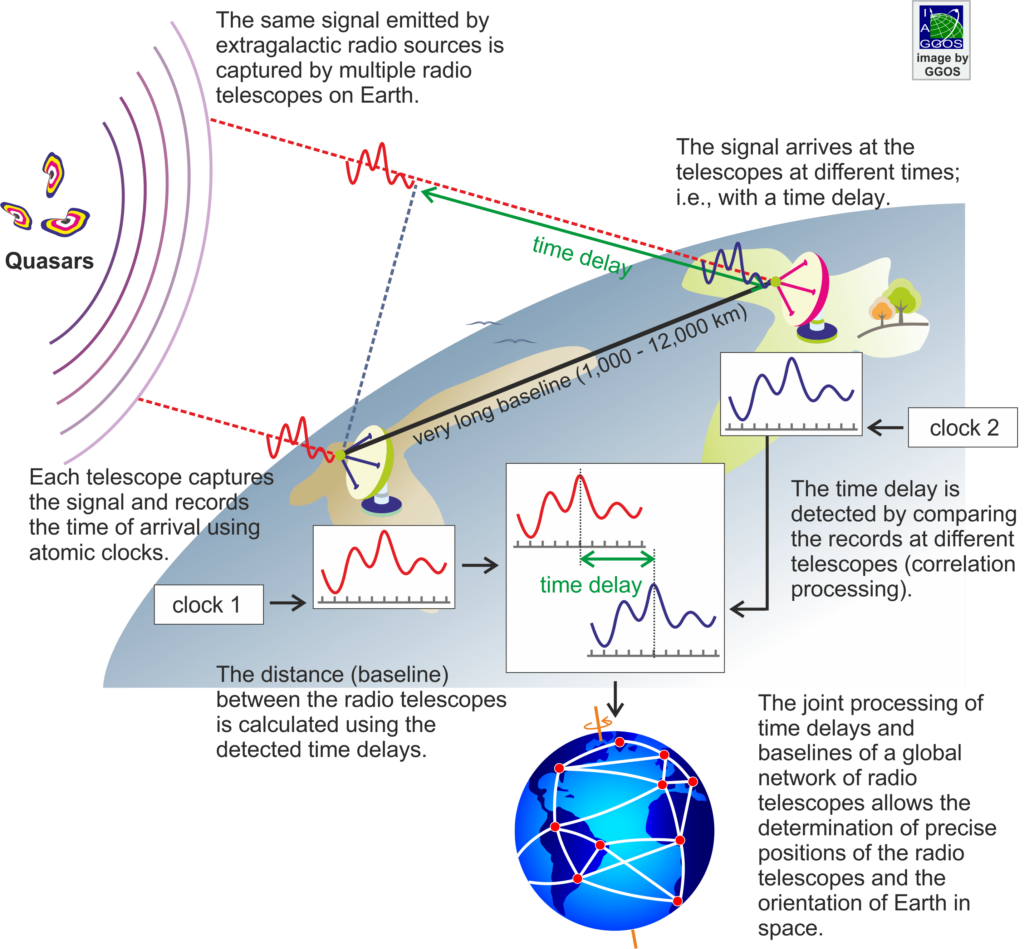
\includegraphics[width=\linewidth]{obs_vlbi_ggos_web_v2-1024x949.png}
    \end{minipage}
    \hfill
    \begin{minipage}[c]{0.54\textwidth}
    \centering
    \begin{tikzpicture}[scale=1.0, >=Stealth]
    % Define the radius and angle
    \def\RE{3.6}
    \def\gammaangle{60}

    % Define coordinates rotated by 90 degrees
    \coordinate (O) at (0,0);
    \coordinate (A) at (90+\gammaangle/2:\RE);
    \coordinate (B) at (90-\gammaangle/2:\RE);
    
    % M is the midpoint of the chord for the perpendicular bisector
    \coordinate (M) at (90:{\RE*cos(\gammaangle/2)});

    % Draw the top arc
    \draw[thick] (0:\RE) arc (0:180:\RE);

    % Draw the radii
    \draw[thick] (O) -- (A) node[midway, left=4pt] {$R_E$};
    \draw[thick] (O) -- (B) node[midway, right=4pt] {$R_E$};

    % Draw the full chord
    \draw[thick, blue] (A) -- (B);

    % Draw the perpendicular bisector
    \draw[thick, dashed, red] (O) -- (M);

    % Right angle marker at the intersection
    \draw (M) ++(0,-0.2) -- ++(0.2,0) -- ++(0,0.2);

    % Label the half-chord distances using braces
    \draw[decorate, decoration={brace, amplitude=5pt, raise=2pt}, thick]
         (A) -- (M) node[midway, above=10pt] {$R_E \sin(\gamma/2)$};
    \draw[decorate, decoration={brace, amplitude=5pt, raise=2pt}, thick]
         (M) -- (B) node[midway, above=10pt] {$R_E \sin(\gamma/2)$};

    % Draw and label the split angles
    \pic [draw, thick, "$\frac{\gamma}{2}$", angle eccentricity=1.6, angle radius=0.9cm] {angle = M--O--A};
    \pic [draw, thick, "$\frac{\gamma}{2}$", angle eccentricity=1.6, angle radius=0.9cm] {angle = B--O--M};

    % Mark and label the points
    \fill (O) circle (2pt) node[below=2pt] {$O$};
    \fill (A) circle (2pt) node[above left] {$P_1$};
    \fill (B) circle (2pt) node[above right] {$P_2$};
    \fill (M) circle (1.5pt) node[below right=1pt] {$M$};
    \end{tikzpicture}
    \end{minipage}
    \caption{Global VLBI network (left) and the chord baseline geometry $C = 2R_E\sin(\gamma/2)$ through the Earth's interior (right).}
    \label{fig:vlbi_chord_geometry}
\end{figure}

The straight-line chord distance is therefore:
\begin{keyresult}
	\begin{equation}
		C = 2R_E\sin\left(\frac{\gamma}{2}\right) = R_E\sqrt{2(1-\cos\gamma)}.
		\label{eq:chord_baseline_formula}
	\end{equation}
\end{keyresult}

\subsection{Derivation of the Baseline Interferometer Angular Resolution Limit}

To understand how an interferometer synthesizes high angular resolution from two antennas separated by a physical baseline $B$, consider two distinct astronomical point sources on the sky, \textbf{Source 1} and \textbf{Source 2}, observed simultaneously at observing wavelength $\lambda$.

\begin{figure}[htbp]
\centering
\begin{tikzpicture}[scale=1.15, >=Stealth]
    \def\B{6.0}
    \def\thOne{20}
    \def\thTwo{42}
    \def\rayLen{5.2}
    
    \coordinate (A1) at (0,0);
    \coordinate (A2) at (\B,0);
    
    % Normal lines
    \draw[dashed, gray!60, thick] (A1) -- (0, 4.8) node[above, gray!80!black] {Normal};
    \draw[dashed, gray!60, thick] (A2) -- (\B, 4.8) node[above, gray!80!black] {Normal};
    
    % Source 1 directions (coming from upper right at angle thOne to normal)
    \pgfmathsetmacro{\sOneX}{\rayLen*sin(\thOne)}
    \pgfmathsetmacro{\sOneY}{\rayLen*cos(\thOne)}
    \coordinate (S1_A1) at (\sOneX, \sOneY);
    \coordinate (S1_A2) at ({\B + \sOneX}, \sOneY);
    
    % Source 2 directions (coming from upper right at angle thTwo to normal)
    \pgfmathsetmacro{\sTwoX}{\rayLen*sin(\thTwo)}
    \pgfmathsetmacro{\sTwoY}{\rayLen*cos(\thTwo)}
    \coordinate (S2_A1) at (\sTwoX, \sTwoY);
    \coordinate (S2_A2) at ({\B + \sTwoX}, \sTwoY);
    
    % Intersection points W1 and W2 on ray A1 from wavefronts starting at Antenna 2 (A2)
    \pgfmathsetmacro{\wOneX}{\B*sin(\thOne)*sin(\thOne)}
    \pgfmathsetmacro{\wOneY}{\B*sin(\thOne)*cos(\thOne)}
    \coordinate (W1) at (\wOneX, \wOneY);
    
    \pgfmathsetmacro{\wTwoX}{\B*sin(\thTwo)*sin(\thTwo)}
    \pgfmathsetmacro{\wTwoY}{\B*sin(\thTwo)*cos(\thTwo)}
    \coordinate (W2) at (\wTwoX, \wTwoY);
    
    % Incoming rays for Source 1 (Red)
    \draw[->, very thick, red!80!black] (S1_A1) -- (A1);
    \draw[->, very thick, red!80!black] (S1_A2) -- (A2);
    
    % Incoming rays for Source 2 (Blue)
    \draw[->, very thick, blue!80!black] (S2_A1) -- (A1);
    \draw[->, very thick, blue!80!black] (S2_A2) -- (A2);
    
    % Wavefronts from Antenna 2 (A2) hitting rays at Antenna 1 at exact 90 degrees
    \draw[dashed, line width=1.1pt, red!80!black] (A2) -- (W1);
    \draw[dashed, line width=1.1pt, blue!80!black] (A2) -- (W2);
    
    % Right angle markers at W1 and W2 (exact 90-degree square markers)
    \pgfmathsetmacro{\sqSize}{0.28}
    \draw[thick, red!80!black] 
        ($(W1) + ({\sqSize*cos(\thOne)}, {-\sqSize*sin(\thOne)})$) -- 
        ++({-\sqSize*sin(\thOne)}, {-\sqSize*cos(\thOne)}) -- 
        ($(W1) + ({-\sqSize*sin(\thOne)}, {-\sqSize*cos(\thOne)})$);
        
    \draw[thick, blue!80!black] 
        ($(W2) + ({\sqSize*cos(\thTwo)}, {-\sqSize*sin(\thTwo)})$) -- 
        ++({-\sqSize*sin(\thTwo)}, {-\sqSize*cos(\thTwo)}) -- 
        ($(W2) + ({-\sqSize*sin(\thTwo)}, {-\sqSize*cos(\thTwo)})$);
        
    % Path lags along ray entering Antenna 1
    \draw[line width=3.0pt, red!80!black] (W1) -- (A1);
    \node[left=4pt, red!80!black, font=\bfseries] at ($(W1)!0.5!(A1)$) {$\Delta L_1 = B\sin\theta_1$};
    
    \draw[line width=3.0pt, blue!80!black] (W2) -- (A1);
    \node[right=4pt, blue!80!black, font=\bfseries] at ($(W2)!0.6!(A1)$) {$\Delta L_2 = B\sin\theta_2$};
    
    % Baseline line
    \draw[line width=1.6pt, ink] (A1) -- (A2) node[midway, below=6pt] {\textbf{Baseline} $B$};
    \fill[astroblue] (A1) circle (3pt) node[below left=2pt] {\textbf{Antenna 1} ($A_1$)};
    \fill[astroblue] (A2) circle (3pt) node[below right=2pt] {\textbf{Antenna 2} ($A_2$)};
    
    % Angle arcs at A2
    \draw[->, thick, red!80!black] (\B, 2.2) arc (90:{90-\thOne}:2.2) node[midway, above] {$\theta_1$};
    \draw[->, thick, blue!80!black] (\B, 3.2) arc (90:{90-\thTwo}:3.2) node[midway, above right] {$\theta_2$};
    
    % Angle arcs at A1
    \draw[->, thick, red!80!black] (0, 2.2) arc (90:{90-\thOne}:2.2) node[midway, above] {$\theta_1$};
    \draw[->, thick, blue!80!black] (0, 3.2) arc (90:{90-\thTwo}:3.2) node[midway, above right] {$\theta_2$};
    
    % Source labels at top
    \node[red!80!black, right=2pt, font=\bfseries] at (S1_A2) {Source 1};
    \node[blue!80!black, right=2pt, font=\bfseries] at (S2_A2) {Source 2};
\end{tikzpicture}
\caption{Geometric optical path delays for two distinct sources observed by a two-element interferometer of baseline $B$. Wavefronts from Antenna 2 ($A_2$) strike the rays entering Antenna 1 ($A_1$) at right angles ($90^\circ$), defining the respective geometric lags $\Delta L_1 = B\sin\theta_1$ and $\Delta L_2 = B\sin\theta_2$.}
\label{fig:interferometer_two_sources}
\end{figure}

Let the directions to the two sources make angles $\theta_1$ and $\theta_2$ with respect to the baseline normal:
\begin{enumerate}
	\item \textbf{Geometric Path Lag for Source 1:} A plane wavefront from Source 1 arrives at Antenna 2 before Antenna 1. The extra path distance that the light must travel to reach Antenna 1 is:
	\begin{equation}
		\Delta L_1 = B\sin\theta_1.
		\label{eq:path_lag_source_1}
	\end{equation}
	\item \textbf{Geometric Path Lag for Source 2:} Similarly, a plane wavefront from Source 2 arrives at angle $\theta_2$, resulting in a geometric path lag to Antenna 1 of:
	\begin{equation}
		\Delta L_2 = B\sin\theta_2.
		\label{eq:path_lag_source_2}
	\end{equation}
	\item \textbf{Differential Path Difference Between the Two Sources:} The net difference in path delay between the signals arriving from the two sources across the baseline is:
	\begin{equation}
		\Delta(\Delta L) = \Delta L_2 - \Delta L_1 = B\left(\sin\theta_2 - \sin\theta_1\right).
		\label{eq:diff_path_difference}
	\end{equation}
	For closely spaced sources on the sky, let $\theta = \theta_2 - \theta_1$ denote their mutual angular separation. Using the small-angle approximation ($\sin\theta_2 - \sin\theta_1 \approx \theta_2 - \theta_1 = \theta$ for angles near the normal):
	\begin{equation}
		\Delta(\Delta L) = B\left(\sin\theta_2 - \sin\theta_1\right) \approx B\theta.
		\label{eq:diff_path_approx}
	\end{equation}
	\item \textbf{Interferometric Resolution Criterion:} In a radio/optical interferometer, incoming wavefronts are correlated to produce sinusoidal interference fringe patterns. For the interferometer to cleanly resolve (distinguish) Source 1 from Source 2, the fringe pattern of Source 2 must shift relative to that of Source 1 by at least \textbf{one full interference fringe cycle} (corresponding to a full phase shift of $\Delta\phi = 2\pi$), which requires an extra path difference of exactly one full wavelength $\lambda$:
	\begin{equation}
		B\left(\sin\theta_2 - \sin\theta_1\right) = B\theta = \lambda.
		\label{eq:interferometer_resolution_condition}
	\end{equation}
\end{enumerate}

Solving Eq.~\eqref{eq:interferometer_resolution_condition} for the limiting angular resolution $\theta_{\rm res}$:
\begin{keyresult}
	\begin{equation}
		\theta_{\rm res} = \frac{\lambda}{B}\quad [\text{radians}] = \frac{\lambda}{B} \times \frac{180 \times 3600}{\pi}'' = 206{,}265\left(\frac{\lambda}{B}\right)\quad [\text{arcseconds}].
		\label{eq:interferometric_resolution_formula}
	\end{equation}
\end{keyresult}
This fundamental equation demonstrates that interferometric resolution depends solely on the ratio of the observing wavelength $\lambda$ to the baseline separation $B$, allowing distributed arrays to synthesize effective apertures thousands of kilometers wide.

\subsection{Worked Example: Interferometric Resolution for the GMRT to Ooty Baseline}

The baseline length $B = C$ determines the synthesized angular resolution as derived above:
\begin{equation}
	\theta \simeq \frac{\lambda}{B}.
	\label{eq:interferometric_res_approx}
\end{equation}

\begin{example}[Interferometry Between GMRT and Ooty Radio Telescope]
	The coordinates $(\phi,\lambda)$ of the Giant Metrewave Radio Telescope (GMRT, Khodad) and Ooty Radio Telescope (ORT) are:
	\[
	\begin{aligned}
		\text{GMRT}:&\quad (19.09^\circ\text{N},\,74.05^\circ\text{E}),\\
		\text{Ooty}:&\quad (11.38^\circ\text{N},\,76.66^\circ\text{E}).
	\end{aligned}
	\]
	\begin{enumerate}
		\item \textbf{Baseline Distance:} Using Eq.~\eqref{eq:earth_central_angle}:
		\[
		\cos\gamma = \sin(19.09^\circ)\sin(11.38^\circ) + \cos(19.09^\circ)\cos(11.38^\circ)\cos(76.66^\circ - 74.05^\circ) \approx 0.9899.
		\]
		The corresponding straight-line chord distance with $R_E = 6371\,\text{km}$ is:
		\[
		C = 2R_E\sin\left(\frac{\gamma}{2}\right) \implies \boxed{C \simeq 904.5\,\mathrm{km}}.
		\]
		\item \textbf{Angular Resolution at $1000\,\mathrm{MHz}$:}
		At observing frequency $f = 1000\,\mathrm{MHz} = 10^9\,\mathrm{Hz}$, the observing wavelength is:
		\[
		\lambda = \frac{c}{f} = \frac{3 \times 10^8\,\mathrm{m/s}}{10^9\,\mathrm{Hz}} = 0.30\,\mathrm{m}.
		\]
		Taking the baseline as $B \simeq 904.5\,\mathrm{km} = 9.045 \times 10^5\,\mathrm{m}$:
		\[
		\theta \simeq \frac{\lambda}{B} = \frac{0.30}{9.045 \times 10^5} \simeq 3.32 \times 10^{-7}\,\mathrm{rad}.
		\]
		Converting to milliarcseconds ($1\,\text{rad} = \frac{180}{\pi} \times 3.6 \times 10^6\,\text{mas} \approx 2.06265 \times 10^8\,\text{mas}$):
		\[
		\boxed{\theta \simeq 3.32 \times 10^{-7}\left(\frac{180}{\pi}\right)(3.6 \times 10^6) \simeq 68.4\,\mathrm{mas}}.
		\]
	\end{enumerate}
\end{example}

\section{Telescope Optics: Cassegrain Geometry, Focal Length, and Scale Relations}

\subsection{Cassegrain Reflector Telescope Geometry}

In a Cassegrain reflector telescope, incoming parallel light rays from infinity hit the concave primary mirror of diameter $D$ and focal length $F$. Before reaching the primary focus, a convex secondary mirror of diameter $b$ intercepts the converging cone at a distance $d$ from the primary, reflecting and focusing the beam through a central hole in the primary mirror onto a detector placed at distance $a$ behind the primary.

\begin{figure}[htbp]
\centering
\resizebox{0.95\textwidth}{!}{
\begin{tikzpicture}[scale=1.0, >=Stealth]
    \def\D{3.0}     % Primary diameter (30 cm scaled)
    \def\d{7.5}     % Mirror distance (0.75 m scaled)
    \def\b{1.875}   % Secondary diameter (18.75 cm scaled)
    \def\a{5.0}     % CCD distance (0.5 m scaled)
    \def\F{-12.5}   % Primary focus (2.0 m scaled -> 20 units left of primary at 7.5)
    
    % Background shading for the similar triangle
    \fill[orange!10] (\d, 1.5) -- (\F, 0) -- (\d, -1.5) -- cycle;
    
    % Virtual rays continuing to the Primary Focus (completes the similar triangle)
    \draw[dotted, orange, ultra thick] (0, \b/2) -- (\F, 0);
    \draw[dotted, orange, ultra thick] (0, -\b/2) -- (\F, 0);
    \fill[orange] (\F, 0) circle (3pt) node[below=2mm] {\Large Focus};
    
    % Mark overall Focal Length (F = 2.0m) at the top
    \draw[|-|, thick, orange] (\F, 2.5) -- (\d, 2.5) node[midway, above] {\Large $F = 2.0\text{ m}$ (Focal Length)};

    % Incoming Rays from infinity (aligned with the edges of the primary mirror)
    \draw[dashed, red, thick, ->] (-3, 1.5) -- (\d, 1.5);
    \draw[dashed, red, thick, ->] (-3, -1.5) -- (\d, -1.5);
    
    % Primary Mirror
    \fill[yellow!60] (\d, 1.5) to[bend left=10] (\d+0.2, 0.5) -- (\d, 0.5) -- cycle;
    \fill[yellow!60] (\d, -1.5) to[bend right=10] (\d+0.2, -0.5) -- (\d, -0.5) -- cycle;
    \draw[ultra thick, green!60!black] (\d, 1.5) to[bend left=10] (\d+0.2, 0.5) -- (\d, 0.5);
    \draw[ultra thick, green!60!black] (\d, -1.5) to[bend right=10] (\d+0.2, -0.5) -- (\d, -0.5);
    
    % Secondary Mirror
    \draw[ultra thick, teal] (0, \b/2) -- (0, -\b/2) node[midway, left=2mm, text=teal] {\Large $b$};
    
    % Reflected converging rays from primary to secondary
    \draw[dashed, red, thick, ->] (\d, 1.5) -- (0, \b/2);
    \draw[dashed, red, thick, ->] (\d, -1.5) -- (0, -\b/2);
    
    % Reflected rays from secondary to CCD
    \draw[dashed, red, thick, ->] (0, \b/2) -- (\d+\a, 0);
    \draw[dashed, red, thick, ->] (0, -\b/2) -- (\d+\a, 0);
    
    % CCD at focal plane
    \draw[ultra thick, blue!80!black] (\d+\a, 0.6) -- (\d+\a, -0.6) node[below=2mm] {\Large CCD};
    \fill[red] (\d+\a, 0) circle (2.5pt);
    
    % Continuous bottom dimension lines showing the geometry
    \draw[|-|, thick, teal] (\F, -2.4) -- (0, -2.4) node[midway, below] {\Large $1.25\text{ m}$};
    \draw[|-|, thick, blue] (0, -2.4) -- (\d, -2.4) node[midway, below] {\Large $0.75\text{ m}$};
    \draw[|-|, thick, blue] (\d, -2.4) -- (\d+\a, -2.4) node[midway, below] {\Large $a = 0.50\text{ m}$};
    
    % Primary Mirror Aperture Dimension
    \draw[|-|, thick, green!60!black] (\d+0.6, -1.5) -- (\d+0.6, 1.5) node[midway, right] {\Large $30\text{ cm}$};
\end{tikzpicture}
}
\caption{Cassegrain reflector telescope: similar-triangle geometry used to compute secondary mirror size $b$ and CCD focal distance $a$.}
\label{fig:cassegrain_geometry}
\end{figure}

\begin{example}[Calculating Dimensions $a$ and $b$ for a Cassegrain Telescope]
	Let the primary mirror have diameter $D = 30\,\mathrm{cm}$ and focal length $F = 2.0\,\mathrm{m}$. The secondary mirror is located at $0.75\,\mathrm{m}$ from the primary.
	\begin{enumerate}
		\item Since the secondary mirror is $0.75\,\mathrm{m}$ from the primary, it lies:
		\[
		F - 0.75\,\mathrm{m} = 1.25\,\mathrm{m}
		\]
		from the primary focus.
		\item Using similar triangles:
		\[
		\frac{b}{D} = \frac{1.25}{2.0} \implies b = 30\left(\frac{1.25}{2.0}\right) = 18.75\,\mathrm{cm}.
		\]
		\item The folded path from the secondary to the focus is $1.25\,\mathrm{m}$. Since the primary--secondary separation is $0.75\,\mathrm{m}$:
		\[
		a = 1.25 - 0.75 = 0.50\,\mathrm{m}.
		\]
	\end{enumerate}
\end{example}

\subsection{Optical Ray Diagram and Angular Resolution on the Focal Plane}

\begin{figure}[htbp]
    \centering
    \begin{tikzpicture}[
        >=Stealth,
        font=\sffamily\small,
        ray/.style={thick, color=black},
        marginal/.style={thin, color=black!25} % Faded style for marginal/off-axis non-chief rays
    ]

        % Coordinates & Parameters
        \coordinate (LensCenter) at (0,0);
        \def\FocalLength{4.5}
        \def\ImageOffset{1.6} % Height y of off-axis image B
        
        \coordinate (ImageA) at (\FocalLength, 0);            % Center focal point (Image A)
        \coordinate (ImageB) at (\FocalLength, \ImageOffset);   % Off-axis focal point (Image B)
        
        % Focal Plane Line & Bottom Text
        \draw[thick] (\FocalLength, -2.5) -- (\FocalLength, 2.5);
        \node[below=4pt, align=center] at (\FocalLength, -2.5) {FOCAL\\PLANE};
        
        % Lens
        \draw[thick, fill=blue!5, draw=black] 
            (-0.25,-1.8) to[out=20, in=-20] (-0.25, 1.8) 
            to[out=-160, in=160] (-0.25,-1.8);

        % Optical Axis (Reference line)
        \draw[dashed, gray!40] (-6,0) -- (\FocalLength+0.5,0);

        % ================= SOURCE A (On-Axis: 3 Rays) =================
        % Ray A1 (Top horizontal ray - Faded)
        \draw[marginal] (-5.5, 0.8) -- (0, 0.8) -- (ImageA);
        \draw[marginal] (-5.5, 0.8) -- (-2.75, 0.8) [arrows={-Stealth}];
        \draw[marginal] (0, 0.8) -- ($(0,0.8)!0.5!(ImageA)$) [arrows={-Stealth}];

        % Ray A2 (Central optical axis ray / Chief Ray - Main Focus)
        \draw[ray] (-5.5, 0) -- (LensCenter) -- (ImageA);
        \draw[ray] (-5.5, 0) -- (-2.75, 0) [arrows={-Stealth}];
        \draw[ray] (LensCenter) -- ($0.5*(LensCenter)+0.5*(ImageA)$) [arrows={-Stealth}];

        % Ray A3 (Bottom horizontal ray - Faded)
        \draw[marginal] (-5.5, -0.8) -- (0, -0.8) -- (ImageA);
        \draw[marginal] (-5.5, -0.8) -- (-2.75, -0.8) [arrows={-Stealth}];
        \draw[marginal] (0, -0.8) -- ($(0,-0.8)!0.5!(ImageA)$) [arrows={-Stealth}];


        % ================= SOURCE B (Off-Axis: 3 Rays at Angle theta) =================
        % Ray B1 (Upper angled ray entering lens at y = 0.7 - Faded)
        \coordinate (B_start_top) at (-5.5, {0.7 - 5.5 * (\ImageOffset / \FocalLength)});
        \draw[marginal] (B_start_top) -- (0, 0.7) -- (ImageB);
        \draw[marginal] (B_start_top) -- ($0.5*(B_start_top)+0.5*(0,0.7)$) [arrows={-Stealth}];
        \draw[marginal] (0, 0.7) -- ($(0,0.7)!0.5!(ImageB)$) [arrows={-Stealth}];

        % Ray B2 (Central chief ray through lens center - Main Focus)
        \coordinate (B_start_chief) at (-5.5, {-5.5 * (\ImageOffset / \FocalLength)});
        \draw[ray] (B_start_chief) -- (LensCenter) -- (ImageB);
        \draw[ray] (B_start_chief) -- ($0.5*(B_start_chief)+0.5*(LensCenter)$) [arrows={-Stealth}];
        \draw[ray] (LensCenter) -- ($0.5*(LensCenter)+0.5*(ImageB)$) [arrows={-Stealth}];

        % Ray B3 (Lower angled ray entering lens at y = -0.7 - Faded)
        \coordinate (B_start_lower) at (-5.5, {-0.7 - 5.5 * (\ImageOffset / \FocalLength)});
        \draw[marginal] (B_start_lower) -- (0, -0.7) -- (ImageB);
        \draw[marginal] (B_start_lower) -- ($0.5*(B_start_lower)+0.5*(0,-0.7)$) [arrows={-Stealth}];
        \draw[marginal] (0, -0.7) -- ($(0,-0.7)!0.5!(ImageB)$) [arrows={-Stealth}];


        % ================= LABELS & MARKS =================
        % Angle theta mark
        \draw [thick] (1.3,0) arc (0:19.5:1.2);
        \node at (1.5, 0.25) {$\theta$};

        % Source & Image Labels
        \node[left] at (-5.5, 0) {FROM SOURCE A};
        \node[left] at (-5.5, -2.2) {FROM SOURCE B};

        \draw[thin] (ImageB) -- (\FocalLength+0.8, 2.0) node[right] {IMAGE OF SOURCE B};
        \draw[thin] (ImageA) -- (\FocalLength+0.8, -0.4) node[right] {IMAGE OF SOURCE A};

        % Dimension y (displacement on focal plane)
        \draw[<->, thick] (\FocalLength+0.3, 0) -- (\FocalLength+0.3, \ImageOffset) 
            node[midway, right] {$y$};
        \draw[thin, gray] (ImageA) -- (\FocalLength+0.4, 0);
        \draw[thin, gray] (ImageB) -- (\FocalLength+0.4, \ImageOffset);

        % Dimension F (focal length)
        \draw[<->, thick] (-0.25, -1.8) -- (\FocalLength, -1.8) 
            node[midway, fill=white, inner sep=2pt] {$F$};
        \draw[thin, gray] (-0.25, -1.5) -- (-0.25, -2.0);
        \draw[thin, gray] (\FocalLength, -0.2) -- (\FocalLength, -2.0);

    \end{tikzpicture}
    \caption{Ray diagram illustrating angular resolution of two point sources, highlighting the central chief rays while marginal rays are faded for visual clarity.}
    \label{fig:telescope_ray_diagram}
\end{figure}

\subsection{Plate Scale and Pixel Scale Formulations}

\paragraph{Plate Scale ($P$):} Plate scale relates the angular field of view of a frame, $d\theta$, (typically measured in arcseconds), to the size of the detector, $ds$, either in terms of a physical dimension (typically millimetres) or per pixel and is defined as:
\begin{keyresult}
	\begin{equation}
		P = \dv{\theta}{s} = \frac{\theta}{y},
		\label{eq:plate_scale_def}
	\end{equation}
\end{keyresult}
where $\theta$ is measured in arcsec ($=\frac{1}{3600}^\circ$).

\paragraph{Pixel Scale ($\theta_{\rm pix}$):} The pixel scale is the angular extent corresponding to a single physical pixel, and can be defined as:
\begin{equation}
	\theta_{\rm pix} = \frac{y_{\rm pix}}{F} = \frac{p}{F}.
	\label{eq:pixel_scale_def}
\end{equation}
From geometry:
\begin{align}
    \tan\theta \approx \theta = \frac{y}{F} \implies \frac{1}{F} = \frac{\theta}{y},
\end{align}
which relates the two scales.

\begin{keyresult}
	For a focal length $F$, a pixel of physical size $p$ subtends the angle:
	\begin{equation}
		\theta_{\rm pix} \simeq \frac{y}{F}\bigg\lvert_{y=p}.
		\label{eq:pixel_scale_lvert}
	\end{equation}
	With $p$ in metres (or $\mu\mathrm{m}$) and $F$ in metres:
	\begin{equation}
		\text{Pixel Scale} = \frac{y}{F}\bigg\lvert_{y=p} \times \frac{180 \times 3600}{\pi}'' = \frac{206{,}265 \times p\,[\mathrm{mm}]}{F\,[\mathrm{mm}]}\quad [\text{arcsec/pixel}].
		\label{eq:pixel_scale_boxed_result}
	\end{equation}
\end{keyresult}

\begin{example}[Pixel Scale for a CCD with $20\,\mu\mathrm{m}$ Pixels]
	With pixel size $p = 20\,\mu\mathrm{m} = 20 \times 10^{-6}\,\mathrm{m}$ and telescope focal length $F = 2\,\mathrm{m}$:
	\[
	\theta_{\rm pix} = \frac{y}{F}\bigg\lvert_{y=p} = \frac{20 \times 10^{-6}\,\mathrm{m}}{2\,\mathrm{m}} = 1.0 \times 10^{-5}\,\mathrm{rad}.
	\]
	Using $1\,\mathrm{rad} = \frac{180 \times 3600}{\pi}'' = 206265''$:
	\[
	\boxed{\theta_{\rm pix} = \frac{y}{F}\bigg\lvert_{y=p} \simeq 2.06''/\mathrm{pixel}}.
	\]
\end{example}

\section{The Physical and Universal Derivation of Optical Resolution Limits}

In wave optics, the resolution limit of an imaging system defines its ability to distinguish two closely spaced point sources. According to the \textbf{Rayleigh Criterion}, two sources are considered just resolved when the central maximum of the diffraction pattern of one source falls directly on the first minimum (dark fringe) of the other. 

While constructive interference requires an optical path difference of $n\lambda$, the boundary of image resolution is fundamentally dictated by the condition for the \textbf{first destructive minimum}, which depends entirely on the geometry of the aperture.

\subsection{Geometric Derivation: The Single Slit ($1.00\lambda$)}

Consider monochromatic light of wavelength $\lambda$ incident normally on a long rectangular slit of width $D$. We seek the angular position $\theta$ of the first minimum on a distant screen:
\begin{enumerate}
    \item \textbf{Slit Subdivision:} Imagine dividing the slit of width $D$ into two equal halves (zones): a top half and a bottom half.
    \item \textbf{Ray Pairing:} For every light ray originating from a point in the top half, there exists a corresponding ray originating from a point exactly $D/2$ below it in the bottom half.
    \item \textbf{Destructive Condition:} For these paired rays to cancel each other out completely, they must arrive out of phase, requiring a local path difference of exactly half a wavelength:
    \begin{equation}
        \Delta x_{\text{pair}} = \frac{\lambda}{2}.
        \label{eq:slit_destructive_condition}
    \end{equation}
    \item \textbf{Geometric Relation:} From the path geometry at a far diffraction angle $\theta$, the path difference between these two zone halves is given by $\frac{D}{2}\sin\theta$. Equating this to the destructive condition:
    \begin{equation}
        \frac{D}{2}\sin\theta = \frac{\lambda}{2} \implies D\sin\theta = \lambda.
        \label{eq:slit_geometric_relation}
    \end{equation}
\end{enumerate}

Thus, the total path difference between the extreme top and bottom edges of a rectangular slit must be exactly \textbf{$1.00\lambda$} to form the first minimum. Using the small-angle approximation ($\sin\theta \approx \theta$):
\begin{keyresult}
	\begin{equation}
	    \theta \approx \frac{\lambda}{D}.
	    \label{eq:single_slit_minimum}
	\end{equation}
\end{keyresult}

\subsection{The Universal Framework: Fourier Optics}

To derive resolution limits arbitrarily for any aperture shape, we deploy \textbf{Fraunhofer Diffraction}. In the far-field region, the electric field amplitude $E(\vec{k})$ on the screen is mathematically the \textbf{2D Fourier Transform} of the aperture transmission function:
\begin{keyresult}
	\begin{equation}
	    E(\vec{k}) = \iint_{\text{Aperture}} A(\vec{r}) e^{-i \vec{k} \cdot \vec{r}} \, d^2r.
	    \label{eq:fourier_optics_integral}
	\end{equation}
\end{keyresult}
Where:
\begin{itemize}
    \item $A(\vec{r})$ is the transmission aperture function ($1$ inside the opening, $0$ outside).
    \item $\vec{r} = (x, y)$ denotes spatial coordinates inside the aperture.
    \item $\vec{k} = (k_x, k_y)$ is the wave vector mapping to angular screen positions, where $k_x = \frac{2\pi}{\lambda}\sin\theta_x$ and $k_y = \frac{2\pi}{\lambda}\sin\theta_y$.
    \item The exponent term $\vec{k} \cdot \vec{r}$ represents the exact optical phase difference ($\phi = \frac{2\pi}{\lambda}\Delta x$) scaled across the aperture geometry.
\end{itemize}

\subsection{Specializing to a Circular Aperture: The Airy Disk ($1.22\lambda$)}

For most astronomical telescopes, cameras, and the human eye, the entrance pupil is a circular aperture of diameter $D$ (radius $R = D/2$). Transforming the universal Fourier integral Eq.~\eqref{eq:fourier_optics_integral} into polar coordinates $(r', \phi')$:
\[
E(\theta) = \int_0^{D/2} r'\,dr' \int_0^{2\pi} e^{-i k r' \sin\theta \cos\phi'}\,d\phi'.
\]
The azimuthal angular integral produces the Bessel function of order zero, $2\pi J_0(k r' \sin\theta)$. Performing the radial integration via $\int x J_0(x)\,dx = x J_1(x)$ yields the \textbf{First-Order Bessel Function of the First Kind} ($J_1$):
\begin{keyresult}
	\begin{equation}
	    I(\theta) = |E(\theta)|^2 = I_0 \left[ \frac{2 J_1\left(\frac{\pi D \sin\theta}{\lambda}\right)}{\frac{\pi D \sin\theta}{\lambda}} \right]^2.
	    \label{eq:airy_disk_intensity}
	\end{equation}
\end{keyresult}
This diffraction pattern is known as the \textbf{Airy Disk}. The first minimum occurs precisely at the first non-zero root of $J_1(x)$, which evaluates to:
\begin{equation}
    x_1 = \frac{\pi D \sin\theta}{\lambda} \approx 3.8317.
    \label{eq:bessel_first_zero}
\end{equation}
Solving explicitly for $\sin\theta$:
\begin{equation}
    \sin\theta = \frac{3.8317}{\pi} \frac{\lambda}{D} \approx 1.21966 \frac{\lambda}{D} \approx 1.22 \frac{\lambda}{D}.
    \label{eq:circular_aperture_sin_theta}
\end{equation}
Applying the small-angle approximation ($\sin\theta \approx \theta$) yields the standard \textbf{Rayleigh Criterion for a Circular Aperture}:
\begin{keyresult}
	\begin{equation}
	    \theta_{\rm Rayleigh} \approx 1.22 \frac{\lambda}{D}\quad [\text{rad}] = 1.22\frac{\lambda}{D}\times\frac{180 \times 3600}{\pi}''\quad [\text{arcsec}].
	    \label{eq:rayleigh_criterion_result}
	\end{equation}
\end{keyresult}

Consequently, due to the curved chord-weighting of the circular geometry, the edge-to-edge optical path difference required to reach the first dark resolving ring scales from $1.00\lambda$ up to exactly \textbf{$1.22\lambda$}.

\subsection{Summary Comparison of Aperture Geometries}

\begin{table}[htbp]
\centering
\small
\begin{tabular}{llll}
\toprule
\textbf{Aperture Geometry} & \textbf{Fourier Transform Result} & \textbf{First Minimum ($\theta$)} & \textbf{Edge-to-Edge Path Difference} \\ 
\midrule
Single Slit (Rectangular)  & $\text{sinc}^2(x)$                 & $\frac{\lambda}{D}$               & $1.00\lambda$                         \\
Circular Hole             & $\left[\frac{2J_1(x)}{x}\right]^2$ & $1.22\frac{\lambda}{D}$           & $1.22\lambda$                         \\ 
\bottomrule
\end{tabular}
\caption{Geometric dependence of resolution limitations, Fourier intensity profiles, and first minimum criteria.}
\label{tab:aperture_resolution_comparison}
\end{table}

\subsection{The Rayleigh Criterion for Point-Source Imaging}

\begin{figure}[htbp]
    \centering
    \begin{tikzpicture}[
    scale=1.1,
    >=stealth,
    declare function={
        sinc(\x) = (\x==0 ? 1 : sin(deg(\x))/\x);
    }
]

    % Geometry Parameters
    % Red peak at x = -1.2, Blue peak at x = 1.2
    % Peak separation alpha = theta_1 = 2.4 units (Rayleigh Criterion)
    \def\xR{-1.2}
    \def\xB{1.2}
    \def\dx{2.4} 

    % Base axis line
    \draw[->, thick] (-6.5,0) -- (6.5,0);

    % Red diffraction pattern: I(x) = (sinc(pi*(x - xR)/dx))^2
    \draw[red, thick, domain=-6.2:4.5, samples=300, smooth] 
        plot (\x, {3.0 * pow(sinc(3.14159 * (\x - \xR) / \dx), 2)});

    % Blue diffraction pattern: I(x) = (sinc(pi*(x - xB)/dx))^2
    \draw[blue, thick, domain=-4.5:6.2, samples=300, smooth] 
        plot (\x, {3.0 * pow(sinc(3.14159 * (\x - \xB) / \dx), 2)});

    % Vertical dashed lines
    \draw[dashed, thick] (\xR, -1.2) -- (\xR, 3.0);
    \draw[dashed, thick] (\xB, -1.2) -- (\xB, 3.0);
    \draw[dashed, thick] ({\xR - \dx}, -1.2) -- ({\xR - \dx}, 0);
    \draw[dashed, thick] ({\xB + \dx}, -1.2) -- ({\xB + \dx}, 0);

    % Bottom arrows explicitly labeling theta_1 = 1.22 lambda / D
    \draw[<->, thick] ({\xR - \dx}, -0.7) -- node[above] {$\theta_1 = 1.22 \frac{\lambda}{D}$} (\xR, -0.7);
    \draw[<->, thick] (\xR, -0.7) -- node[above] {$\theta_1 = 1.22 \frac{\lambda}{D}$} (\xB, -0.7);
    \draw[<->, thick] (\xB, -0.7) -- node[above] {$\theta_1 = 1.22 \frac{\lambda}{D}$} ({\xB + \dx}, -0.7);

    % Labels and pointer lines
    % Red central maximum label
    \draw[thin] (-1.5, 3.3) -- (\xR, 3.0);
    \node[red, font=\bfseries\sffamily, left] at (-1.5, 3.3) {central maximum};

    % Blue central maximum label
    \draw[thin] (1.5, 3.3) -- (\xB, 3.0);
    \node[blue, font=\bfseries\sffamily, right] at (1.5, 3.3) {central maximum};

    % Blue first minimum label (coincident with Red central peak)
    \draw[thin] (-1.8, 0.7) -- (\xR, 0.05);
    \node[blue, font=\bfseries\sffamily, left] at (-1.8, 0.7) {first minimum};

    % Red first minimum label (coincident with Blue central peak)
    \draw[thin] (1.8, 0.7) -- (\xB, 0.05);
    \node[red, font=\bfseries\sffamily, right] at (1.8, 0.7) {first minimum};

    \end{tikzpicture}
    \caption{Diffraction patterns of two barely resolved point sources under the Rayleigh criterion, where the central maximum of one source coincides with the first minimum ($\theta_1 = 1.22\lambda/D$) of the second.}
    \label{fig:rayleigh_diffraction_sinc}
\end{figure}

\begin{figure}[htbp]
    \centering
    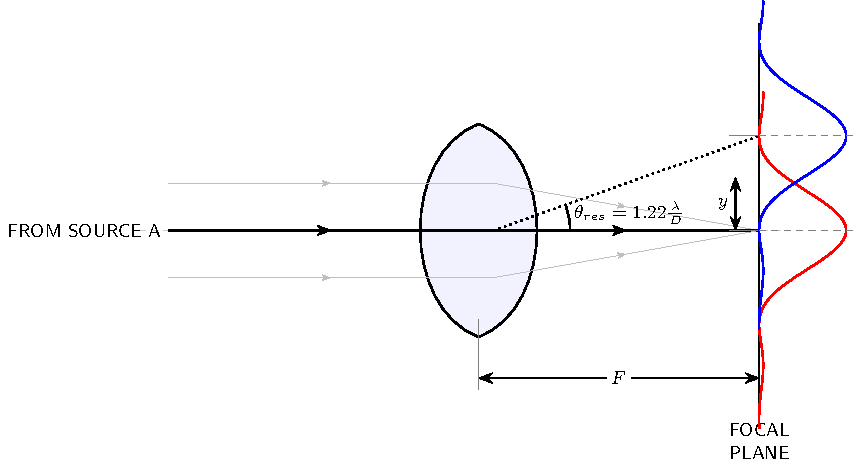
\includegraphics[width=0.6\linewidth]{Diffraction.pdf}
    \caption{Ray optics focusing through a circular entrance pupil and the resulting rotated Airy diffraction profile in the focal plane.}
    \label{fig:diffraction_pdf_diagram}
\end{figure}

\begin{example}[Diffraction Resolution at $\lambda = 500\,\mathrm{nm}$]
	For an optical telescope with aperture $D = 0.30\,\mathrm{m}$ observing at $\lambda = 500\,\mathrm{nm} = 500 \times 10^{-9}\,\mathrm{m}$:
	\[
	\theta_{\rm diff} = 1.22\frac{500 \times 10^{-9}}{0.30} \times \frac{180 \times 3600}{\pi}'' \simeq 2.03 \times 10^{-6} \times 206265'' = 0.42''.
	\]
\end{example}

\section{Comparing Pixel Scale to the Diffraction Limit: Nyquist Sampling}

\subsection{The Nyquist Sampling Criterion}

To record all spatial information contained in the image without aliasing, the \textbf{Nyquist sampling criterion} requires:
\begin{keyresult}
	\begin{equation}
		\text{Pixel Scale} \le \frac{\theta_{\rm res}}{2}.
		\label{eq:nyquist_sampling_criterion}
	\end{equation}
\end{keyresult}
That is, there must be at least \textbf{two detector pixels across the resolution element} ($\mathrm{FWHM} \approx \theta_{\rm res}$).

\subsection{Configuration Critique: Comparison of Pixel Scale and Diffraction Limit}

In the telescope configuration analyzed above:
\begin{itemize}
	\item The pixel scale is:
	\[
	\text{Pixel Scale} = \frac{y}{F}\bigg\lvert_{y=p} = 2.06''/\mathrm{pixel}.
	\]
	\item The diffraction-limited resolution is:
	\[
	\theta_{\rm res} = 1.22\frac{\lambda}{D} = 0.42''.
	\]
\end{itemize}
The Nyquist sampling criterion requires:
\[
\text{Pixel Scale} \le \frac{\theta_{\rm res}}{2} = \frac{0.42''}{2} = 0.21'',
\]
which is \textbf{not respected}. 

Evaluating the ratio of the two quantities:
\begin{keyresult}
	\begin{equation}
		\frac{\text{Pixel Scale}}{\theta_{\rm res}} = \frac{2.06}{0.42} \simeq 4.9.
		\label{eq:pixel_diffraction_ratio}
	\end{equation}
\end{keyresult}
Thus, \textbf{one pixel covers almost five diffraction-limited resolution elements}, which represents a severely \emph{undersampled} configuration. High spatial frequencies are permanently lost to digital aliasing, and point sources cannot be astrometrically centroided to sub-diffraction accuracy.

\begin{table}[htbp]
	\centering
	\small
	\begin{tabular}{lp{5.5cm}p{6.0cm}}
		\toprule
		\textbf{Sampling Regime} & \textbf{Condition} & \textbf{Observational Consequences} \\
		\midrule
		\textbf{Critically Sampled} & $\text{Pixel Scale} \approx \theta_{\rm res}/2$ & Preserves all spatial frequencies without wasting detector area. \\
		\textbf{Undersampled} & $\text{Pixel Scale} > \theta_{\rm res}/2$ & Causes aliasing, jagged stellar profiles, and astrometric centroid degradation. \\
		\textbf{Oversampled} & $\text{Pixel Scale} \ll \theta_{\rm res}/2$ & Spreads light over excessive pixels, increasing total readout noise penalty $\sqrt{n_{\rm pix}}\sigma_{\rm RON}$. \\
		\bottomrule
	\end{tabular}
	\caption{Comparison of digital detector sampling regimes in astronomical imaging.}
	\label{tab:sampling_regimes}
\end{table}

\section{Atmospheric Seeing, PSF Profiles, and Adaptive Optics}

\subsection{Atmospheric Seeing and the Fried Parameter ($r_0$)}

For ground-based optical telescopes, turbulent temperature and density variations in the Earth's atmosphere distort incoming plane wavefronts. The spatial scale over which wavefront phases remain coherent is parameterized by the \textbf{Fried coherence parameter} $r_0$ (typically $r_0 \sim 10\text{--}20\,\mathrm{cm}$ in the $V$-band at premier mountain observatories).

For any telescope with aperture diameter $D > r_0$, the delivered angular resolution is limited not by $D$, but by $r_0$:
\begin{keyresult}
	\begin{equation}
		\theta_{\rm seeing} \approx 0.98\frac{\lambda}{r_0} \sim 0.5''\text{--}1.5''.
		\label{eq:seeing_resolution}
	\end{equation}
\end{keyresult}
Because $r_0 \propto \lambda^{6/5}$, seeing improves at infrared wavelengths ($\theta_{\rm seeing} \propto \lambda^{-1/5}$).

\subsection{Point Spread Function (PSF) Profiles: The Moffat Function}

Turbulent atmospheric scattering smears the theoretical Airy disk into a broader Point Spread Function (PSF). Astronomers parameterize this profile using the \textbf{Moffat function}:
\begin{equation}
	I(r) = I_0 \left[1 + \left(\frac{r}{\alpha}\right)^2\right]^{-\beta}, \qquad \mathrm{FWHM} = 2\alpha\sqrt{2^{1/\beta}-1},
	\label{eq:moffat_function}
\end{equation}
where $\beta \approx 2.5\text{--}4.5$ captures the extended scattering wings produced by Kolmogorov turbulence.

\subsection{Adaptive Optics (AO)}

Adaptive Optics systems restore diffraction-limited performance to ground-based telescopes in real time:
\begin{enumerate}
	\item A \textbf{Wavefront Sensor} (e.g., Shack--Hartmann lenslet array) measures instantaneous phase distortions $\Delta\phi(\mathbf r, t)$ at kHz frequencies using a bright Natural Guide Star (NGS) or Sodium Laser Guide Star (LGS, $\lambda = 589\,\mathrm{nm}$ resonant excitation at $\sim 90\,\mathrm{km}$ altitude).
	\item A real-time computer calculates the required phase conjugation.
	\item A \textbf{Deformable Mirror} (with hundreds to thousands of piezoelectric actuators) physically adjusts its surface profile to cancel out the atmospheric optical path difference.
\end{enumerate}
This restores the sharp $\theta \approx \lambda/D$ diffraction core on 8--30 meter class telescopes, providing space-quality resolution from the ground.

\chapter{The Two-Body Problem}
	
\section{Central Force Problem and Conservation Laws}

\subsection{Central force problem}
	A central force acts along the line joining two particles and depends only on their separation $r=|\vecx_1-\vecx_2|$. Such a force is a gradient of a scalar potential $V(r)$:
	\[
	\vecF(\vecx_1,\vecx_2) = \nabla V(r).
	\]
	Newton's equations for the pair are
	\begin{equation}
		\frac{d^2}{dt^2}\begin{bmatrix}m_1 & 0\\0&m_2\end{bmatrix}\begin{bmatrix}\vecx_1\\\vecx_2\end{bmatrix}
		=\begin{bmatrix}-\nabla V(r)\\ \nabla V(r)\end{bmatrix}. \label{eq:eom2}
	\end{equation}
	Six second-order ODEs $\Rightarrow$ 12 constants of integration in the general solution.
	
	\subsection{Separating centre-of-mass motion}
	\label{sec:com_separation}
	With $M=m_1+m_2$, $\mu = m_1m_2/M$, transform to relative and centre-of-mass coordinates,
	\[
	\begin{bmatrix}\vecr\\ \vec X\end{bmatrix}=\begin{bmatrix}1&-1\\ m_1/M& m_2/M\end{bmatrix}\begin{bmatrix}\vecx_1\\\vecx_2\end{bmatrix},
	\qquad
	\begin{bmatrix}\vecx_1\\\vecx_2\end{bmatrix}=\begin{bmatrix}m_2/M&1\\-m_1/M&1\end{bmatrix}\begin{bmatrix}\vecr\\\vec X\end{bmatrix}.
	\]
	Substituting into \eqref{eq:eom2} and left-multiplying by $\begin{bmatrix}m_2/M&-m_1/M\\1&1\end{bmatrix}$ diagonalizes the mass matrix and decouples the two sectors:
	\begin{align}
		\mu\,\ddot{\vecr} &= -\nabla V(r), \label{eq:relEOM}\\
		M\,\ddot{\vec X} &= 0. \label{eq:comEOM}
	\end{align}
	Equation \eqref{eq:comEOM} integrates trivially: $\vec X(t) = (\vec P/M)t+\vec X_0$, with $\vec P,\vec X_0$ six constants fixing the inertial frame in which the barycentre is at rest at the origin. Everything of dynamical interest is in the \emph{relative} coordinate $\vecr$, governed by \eqref{eq:relEOM} — a one-body central-force problem with reduced mass $\mu$.
	
	\subsection{Conserved quantities}
	
	\paragraph{Angular momentum.} Define $\vecL=\vecr\times\vecp=\mu\,\vecr\times\dot{\vecr}$. Then, because we are considering central force $\ddot{\vec r}\propto \hat{r}$ and hence,
	\[
	\dot{\vecL} = \mu\big[\dot{\vecr}\times\dot{\vecr}+\vecr\times\ddot{\vecr}\big]=0.
	\]
	$\vecL$ supplies three constants of motion: its magnitude $L$, and two angles fixing its direction — the \textbf{inclination} $\iota$ and \textbf{longitude of ascending node} $\Omega$ (Euler angles of the orbital plane relative to a reference plane). Conservation of $\vecL$ confines the motion to the plane $\perp\vecL$.
	
	\paragraph{Energy.} $E=K+V$ with $K=\tfrac12\mu\dot{\vecr}^2$ (the centre-of-mass kinetic term is a constant and drops out). Then
	\[
	\dot E = \mu\dot{\vecr}\cdot\ddot{\vecr}+\dot V
	=\mu\dot{\vecr}\cdot\ddot{\vecr}+\nabla V\cdot\dot{\vecr}
	=\big(\mu\ddot{\vecr}+\nabla V\big)\cdot\dot{\vecr}=0
	\]
	by \eqref{eq:relEOM}. So $E$ is conserved for \emph{any} central potential $V(r)$, not just gravity. Therefore, \textbf{total energy and angular momentum} constitutes four constant of integration. We will learn that there is one more, known as Runge Lenz vector which points towards periapsis and hence encodes the orientation of periapsis and the last constant of integration which is needed specifies the initial phase of the relative orbit ($t_p$)
	\[
	\underbrace{\mathbf R_0,\mathbf V_{\rm CM}}_{6}
	+
	\underbrace{a,e,i,\Omega,\omega,t_p}_{6}
	=12.
	\]
	
	\section{Coordinate Systems and Orbital Elements}
	\label{sec:coord_orbital_elements}

	Fix an equatorial (reference) frame with $\hat\Upsilon$ (vernal equinox / first point of Aries) along $X$ and celestial north $\hat N$ along $Z$; $\hat Y$ completes the right-handed triad. For a source at $(\mathrm{RA},\mathrm{DEC})=(\alpha,\delta)$ the line of sight is
	\[
	\hat R = \cos\delta\cos\alpha\,\hat\Upsilon+\cos\delta\sin\alpha\,\hat Y+\sin\delta\,\hat N,
	\]
	with in-sky-plane axes (pointing along increasing RA, DEC)
	\[
	\hat\alpha=\frac{\pdv{\hat R}{\alpha}}{\abs{\pdv{\hat R}{\alpha}}}=-\sin\alpha\,\hat\Upsilon+\cos\alpha\,\hat Y,\qquad
	\hat\delta=\frac{\pdv{\hat R}{\delta}}{\abs{\pdv{\hat R}{\delta}}}=-\sin\delta\cos\alpha\,\hat\Upsilon-\sin\delta\sin\alpha\,\hat Y+\cos\delta\,\hat N.
	\]
	
	The orbital plane has its own frame: origin at the barycentre, $X$-axis along the \textbf{line of nodes} (through the ascending node and the descending node), $Z$-axis along $\vecL$. Denote the unit vector towards the ascending node by $\hatn$. Then (doing anticlockwise passive rotation)
	
	\begin{equation}
		\begin{pmatrix} \hatn\\ \hat y\\ \hat L \end{pmatrix} =
		\begin{pmatrix} 1&0&0\\ 0&\cos\iota&\sin\iota\\ 0&-\sin\iota&\cos\iota \end{pmatrix} \begin{pmatrix} \cos\Omega&\sin\Omega&0\\ -\sin\Omega&\cos\Omega&0\\ 0&0&1 \end{pmatrix} \begin{pmatrix} \hat\alpha\\ \hat\delta\\ \hat R \end{pmatrix}.
		\label{eq:orbital_frame_rotation}
	\end{equation}
	Hence,
	\begin{align}
		\hatn  &= \cos\Omega\,\hat\alpha+\sin\Omega\,\hat\delta, \label{eq:node}\\
		\hat y &= -\sin\Omega\cos\iota\,\hat\alpha+\cos\Omega\cos\iota\,\hat\delta+\sin\iota\,\hat R, \label{eq:yhat}\\
		\hat L &= \sin\Omega\sin\iota\,\hat\alpha-\cos\Omega\sin\iota\,\hat\delta+\cos\iota\,\hat R, \label{eq:Lhat}
	\end{align}
	\begin{figure}[htbp]
		\centering
		\tdplotsetmaincoords{70}{120}
		\resizebox{\textwidth}{!}{
			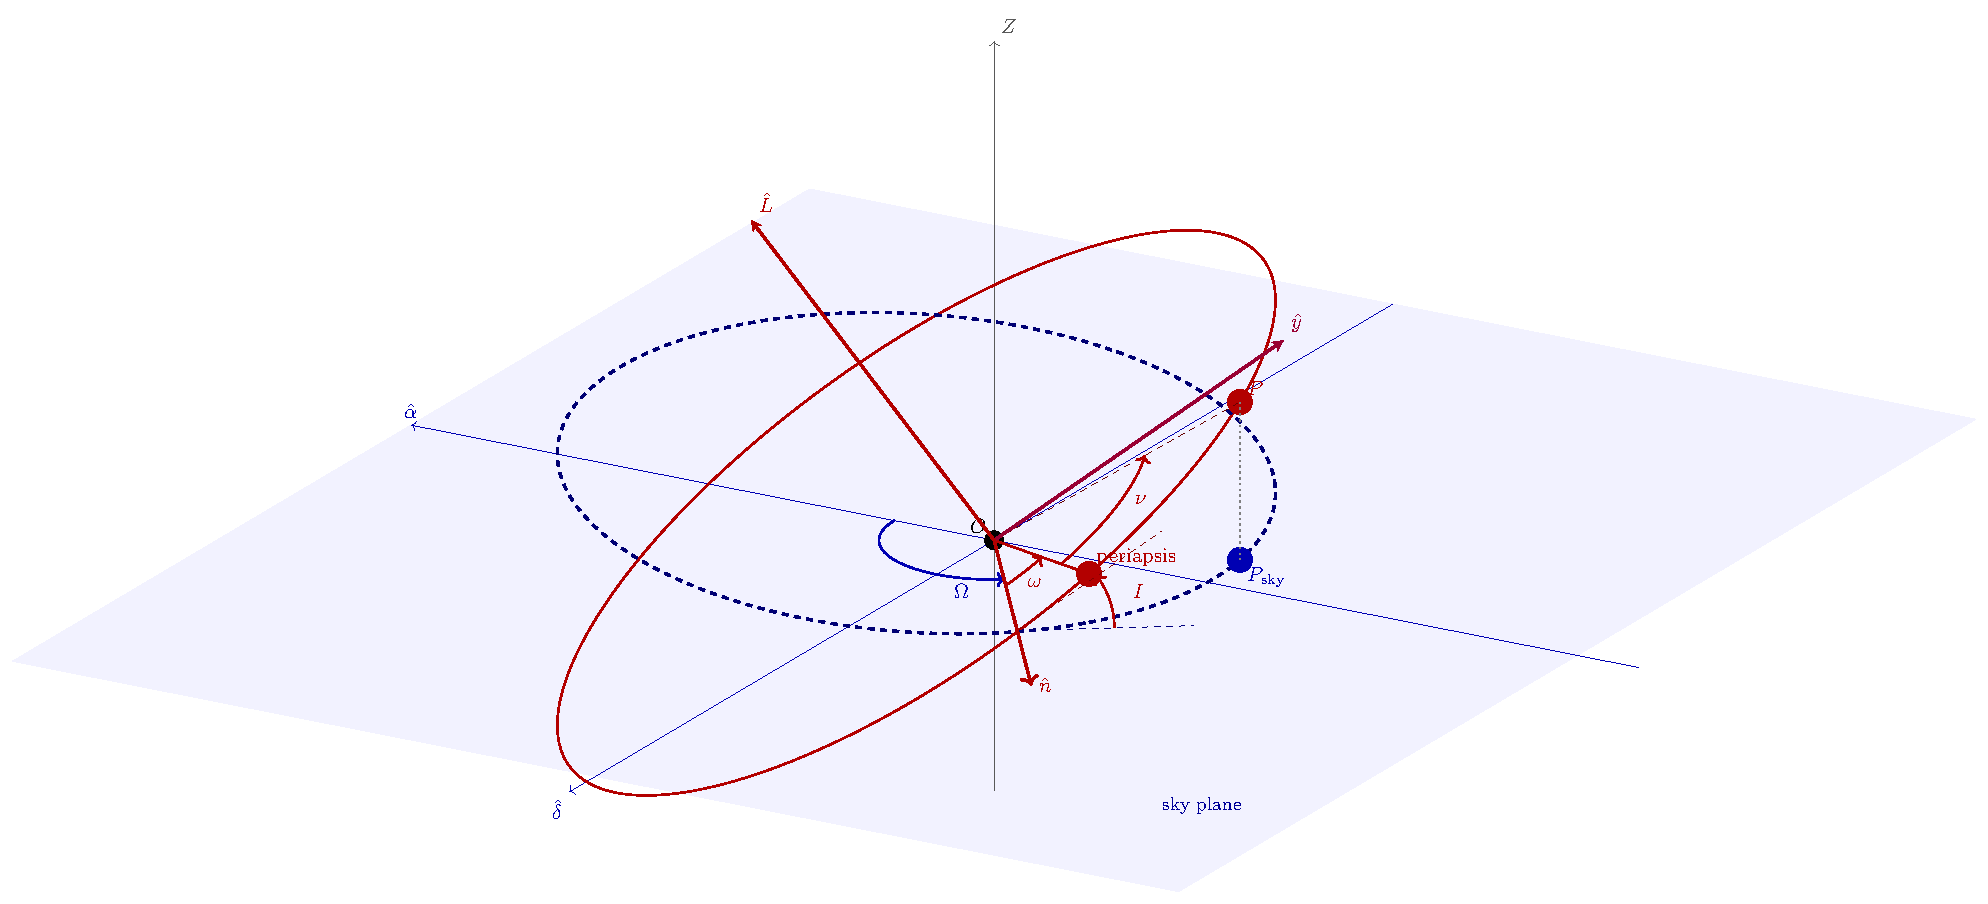
\includegraphics{fig_ch6_orbital_frame_3d.pdf}}
		\caption{Orientation of an orbit relative to sky plane. $\Omega$ (longitude of ascending node) is measured from the reference direction $\alpha$ to the ascending node along the sky plane; $\omega$ (argument of periapsis) is measured from the ascending node to perigee \emph{within} the orbital plane; $\iota$ (inclination) is the dihedral angle between the two planes, read off at the node; $\nu$ (true anomaly) is measured from perigee to the heavenly body's current position. This is exactly $(\Omega,\iota,\omega)$ of Eqs.~\eqref{eq:node}--\eqref{eq:yhat} describe.}
		\label{fig:elements}
	\end{figure}
	so that $\iota=\arccos(\hat L\cdot\hat R)$ is the angle between orbital and reference planes, and $(\hatn,\hat y,\hat L)$ is a right-handed orthonormal triad spanning the orbital plane plus its normal. In this plane use polar coordinates $(r,\phi)$ measured from $\hatn$:
	
	\begin{equation}
		\rhat=\cos\phi\,\hatn+\sin\phi\,\hat y,\qquad
		\phihat=-\sin\phi\,\hatn+\cos\phi\,\hat y. \label{eq:rhat_phihat}
	\end{equation}
	\paragraph{The projected orbit in the sky plane}: If the object in its orbital plane as the coordinate $(r\cos(\omega+\nu),r\sin(\omega+\nu))$, the corresponding coordinate in the sky plane could be found as (clockwise passive rotation):
	
	\begin{align}
		\begin{pmatrix}
			X \\
			Y \\
			Z
		\end{pmatrix}_{\text{Sky Plane}}= 
		\begin{pmatrix}
			\cos\Omega & -\sin\Omega & 0 \\
			\sin\Omega & \cos\Omega & 0 \\
			0 & 0 & 1
		\end{pmatrix}
		\begin{pmatrix}
			1 & 0 & 0 \\
			0 & \cos i & -\sin i \\
			0 & \sin i & \cos i
		\end{pmatrix}
		\begin{pmatrix}
			r\cos(\omega+\nu) \\
			r\sin(\omega+\nu) \\
			0
		\end{pmatrix}_{\text{Orbital Plane}}.
	\end{align}
	Then,
	\begin{align}
		X &= r\left(\cos(\omega+\nu)\cos\Omega-\sin (\omega+\nu)\sin\Omega\cos i\right),\\
		Y &= r\left(\cos(\omega+\nu)\sin\Omega+\sin (\omega+\nu)\cos\Omega\cos i\right).
	\end{align}
	\begin{figure}[htbp]
		\centering
		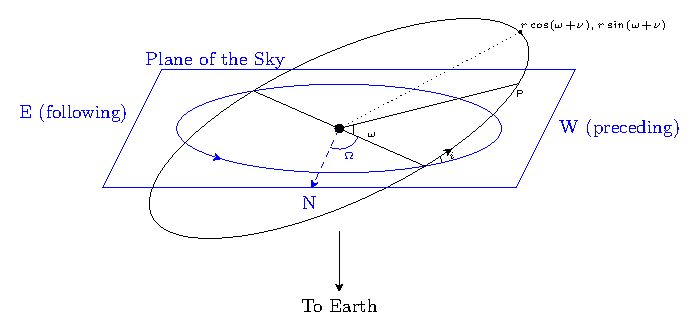
\includegraphics{fig_ch6_conic_sections_geometry.pdf}
		\caption{In this North becomes the local $X$ axis and West becomes the $Y$ axis of the sky plane.}	
	\end{figure}
	
	One can set $\Omega=0$ by another set of basis in the sky plane and then the analysis simplifies immensely
	\begin{align}
		X &= r\cos(\omega+\nu),\\
		Y &= r\sin (\omega+\nu)\cos i.
	\end{align}
	We find that the semi minor axis shrinks by the factor of $\cos i$.
	\paragraph{The six orbital elements.} As the orbit solution unfolds below, six constants emerge in total: $\Omega,\iota$ (orientation of the plane, from $\vecL$), $a,e$ (size and shape, from $E,L$), $\omega$ (orientation of the ellipse \emph{within} the plane, the \textbf{argument of periapsis}), and $T_0$ (time of periapsis passage, fixing where on the ellipse the body is at a given time). Figure~\ref{fig:elements} shows all of these together.
	
	\section{Planar Motion and Kepler's Second Law}
	
	\paragraph{Areal velocity.} The area swept by $\vecr$ in time $dt$ is $dA=\int_{0}^{2\pi}\int_{0}^{r(\phi)} r drd\phi=\frac{1}{2}\int_{0}^{2\pi}r^2(\phi)d\phi$, so
	\begin{equation}
		\frac{dA}{dt}=\frac{r^2\dot\phi}{2} = \frac{L}{2\mu} = \text{const.} \label{eq:kepler2}
	\end{equation}
	This is \textbf{Kepler's second law}: equal areas in equal times. It follows purely from $\vecL$ being conserved, i.e.\ from the force being central — no dependence on the specific form of $V(r)$.
	
	\paragraph{Equations of motion in $(r,\phi)$.} With $Z\parallel\vecL$ and $X\parallel\hatn$, $\vecr=r\rhat$, and
	\[
	\dot{\vecr}=\dot r\,\rhat+r\dot{\hat{r}}=\dot r\,\rhat+r\dot\phi\,\phihat,\qquad
	\ddot{\vecr}=\big(\ddot r-r\dot\phi^2\big)\rhat+\big(2\dot r\dot\phi+r\ddot\phi\big)\phihat.
	\]
	where we used $\nabla_{\mu}\mathbf{e}_{\nu}=\Gamma^{\alpha}_{\mu\nu}\mathbf{e}_{\alpha}$ which gives $\dv{\hat{r}}{t}=\pdv{\hat{r}}{\phi}\dot{\phi}=\dot{\phi}\Gamma_{\phi r}^{\mu}\mathbf{e}_{\mu}=\dot{\phi}\frac{\mathbf{e}_{\phi}}{r}=\dot{\phi}\hat{\phi}$. 
	\begin{figure}
		\centering
		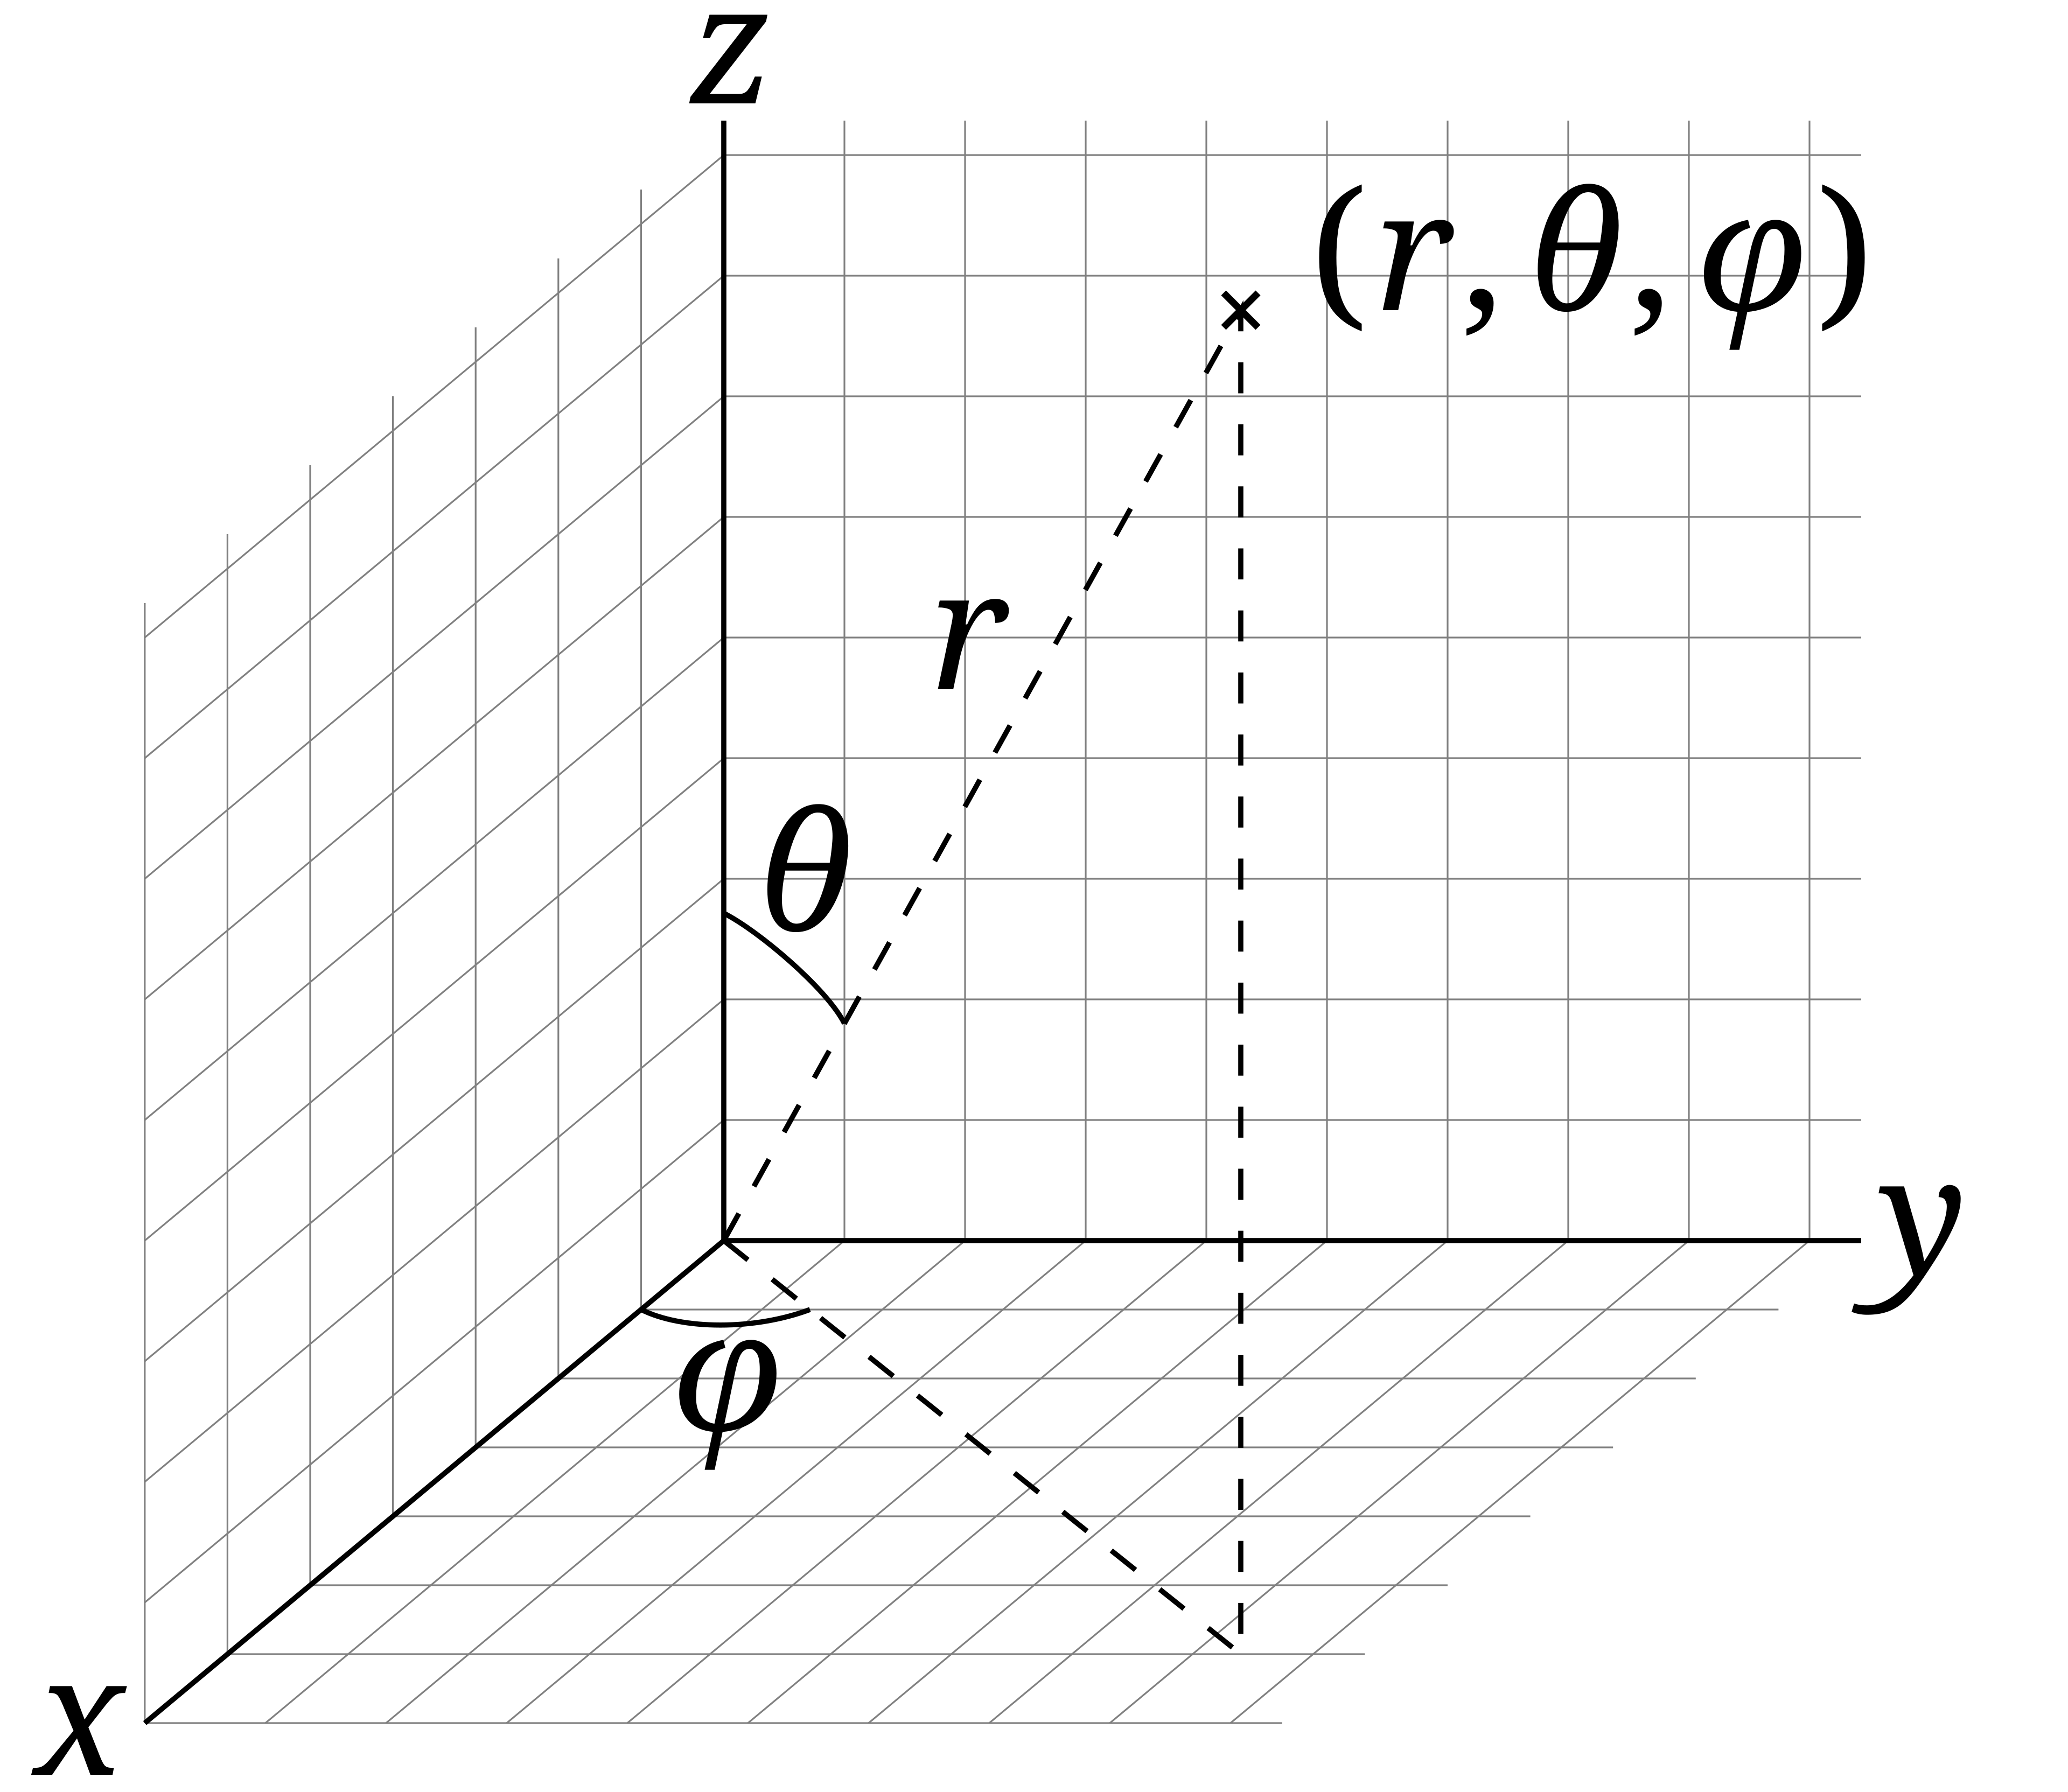
\includegraphics[width=0.5\linewidth]{3D_Spherical.png}
		\caption{Schematic description of spherical polar coordinates.}
		\label{fig:3D_spherical}
	\end{figure}
	Equation \eqref{eq:relEOM} splits into radial and tangential parts:
	\begin{align}
		\mu\big(\ddot r-r\dot\phi^2\big) &= -\nabla V(r), \label{eq:radial}\\
		\mu\big(2\dot r\dot\phi+r\ddot\phi\big) &= 0\implies \dv{(r^2\dot{\phi})}{t}=0. \label{eq:tangential}
	\end{align}
	This was supposed to be a coupled differential equation. But because of equation \eqref{eq:tangential} is just angular momentum conservation, i.e. Kepler's second law again, since $\vecL=\mu\vecr\times\dot{\vecr}=\mu r^2\dot\phi\,\hat L$. So
	\begin{equation}
		\dot\phi = \frac{L}{\mu r^2}, \label{eq:phidot}
	\end{equation}
	and \eqref{eq:radial} becomes, eliminating $\dot\phi$,
	\begin{equation}
		\mu\ddot r - \frac{L^2}{\mu r^3} = -\nabla V(r). \label{eq:radial_reduced}
	\end{equation}
	
	\section{The Orbit Equation}
	
	To get the orbit \emph{shape} $r(\phi)$ we change independent variable from $t$ to $\phi$ using \eqref{eq:phidot}: $\dfrac{dr}{dt}=\dot\phi\dfrac{dr}{d\phi}=\dfrac{L}{\mu r^2}\dfrac{dr}{d\phi}$, and
	\[
	\frac{d^2r}{dt^2}=\frac{L}{\mu r^2}\frac{d}{d\phi}\!\left[\frac{L}{\mu r^2}\frac{dr}{d\phi}\right]
	=\frac{L^2}{\mu^2 r^4}\left[\frac{d^2r}{d\phi^2}-\frac{2}{r}\left(\frac{dr}{d\phi}\right)^2\right].
	\]
	Substituting into \eqref{eq:radial_reduced} and dividing by $L^2/(\mu r^4)$:
	\[
	\frac{1}{r^4}\left[\frac{d^2r}{d\phi^2}-\frac{2}{r}\left(\frac{dr}{d\phi}\right)^2\right]-\frac{1}{r^3}=-\frac{\mu}{L^2}\nabla V(r).
	\]
	The standard trick is the \textbf{Binet substitution} $r=1/\rho$: then $dr/d\phi=-\rho^{-2}d\rho/d\phi$ and $d^2r/d\phi^2=-\rho^{-2}d^2\rho/d\phi^2+2\rho^{-3}(d\rho/d\phi)^2$. Substituting and simplifying (the $(d\rho/d\phi)^2$ terms cancel), one obtains the \textbf{orbit equation}:
	\begin{equation}
		\boxed{\frac{d^2\rho}{d\phi^2}+\rho = \frac{\mu}{L^2}\frac{1}{\rho^2}\nabla V\!\left(\frac1\rho\right).} \label{eq:orbiteq}
	\end{equation}
	This is a purely geometric ODE for the orbit's shape, valid for any central potential.
	
	\section{Keplerian Orbits}
	
	For Newtonian gravity, $V(r)=-GM\mu/r$, so $\nabla V(r) = GM\mu\rho^2\,\rhat$. Equation \eqref{eq:orbiteq} becomes
	\[
	\frac{d^2\rho}{d\phi^2}+\rho =\frac{GM\mu^2}{L^2}.
	\]
	
	Shifting $\tilde\rho=\rho-GM\mu^2/L^2$ turns this into the simple-harmonic-oscillator equation $\ddot{\tilde\rho}+\tilde\rho=0$ (derivatives in $\phi$), with solution $\tilde\rho=A\cos(\phi-\omega)$ for constants $A,\omega$. In terms of $r=1/\rho$:
	\[
	r(\phi)=\left(\frac{GM\mu^2}{L^2}+A\cos(\phi-\omega)\right)^{-1}
	=\frac{L^2/(GM\mu^2)}{1+\dfrac{L^2A}{GM\mu^2}\cos(\phi-\omega)}.
	\]
	Defining the \textbf{semi-latus rectum} $\lambda \equiv L^2/(GM\mu^2)$ as the value of $r$ when $\phi=\omega+90^{\circ}$ and \textbf{eccentricity} $e\equiv \lambda A$,
	\begin{equation}
		\boxed{r(\phi) = \frac{\lambda}{1+e\cos(\phi-\omega)}.} \label{eq:conic}
	\end{equation}
	This is the polar equation of a conic section with one focus at the origin, semi-latus rectum $\lambda$, eccentricity $e$, and major axis rotated by $\omega$ (the \textbf{argument of periapsis} — periapsis occurs at $\phi=\omega$). 
	\begin{figure}[htbp]
		\centering
		
		
		\usetikzlibrary{calc} %allows coordinate calculations
		
		% Newcommand
		
		%% Midline Label
		\newcommand{\midlinelabel}[3]{
			\node (midlabel) at ($ (#1)!.5!(#2) $) {#3};
			\draw[stealth-] (#1) --  (midlabel);
			\draw[-stealth] (midlabel) -- (#2);
		}
		%
		\newcommand{\midlinelabell}[3]{
			\node[fill = white, inner sep = 0.2pt, outer sep=3pt] (midlabel) at ($ (#1)!.5!(#2) $) {#3};
			\draw[stealth-] (#1) --  (midlabel);
			\draw[-stealth] (midlabel) -- (#2);
		}
		\newcommand{\midlinelabelll}[3]{
			\node[fill = white, inner sep = 0.2pt, outer sep=3pt,scale=0.6] (midlabel) at ($ (#1)!.5!(#2) $) {#3};
			\draw[stealth-] (#1) --  (midlabel);
			\draw[-stealth] (midlabel) -- (#2);
		}\usetikzlibrary{calc}
		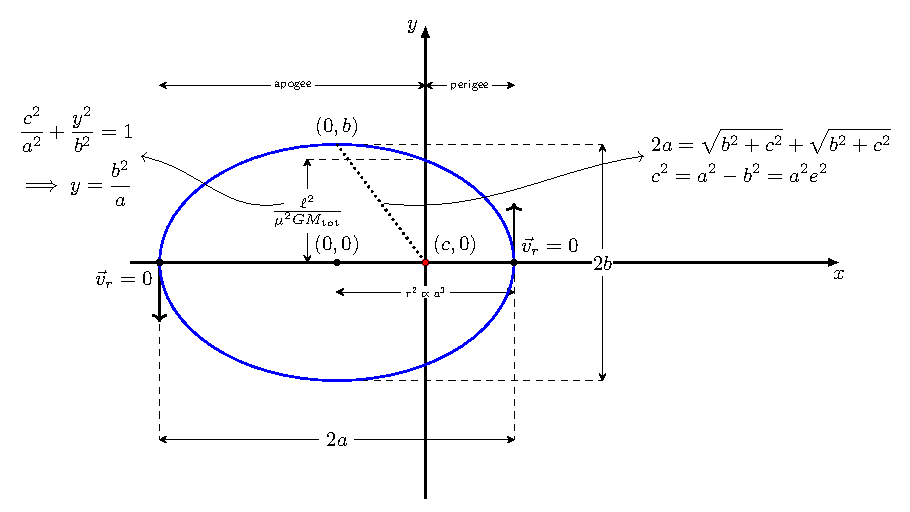
\includegraphics{fig_ch6_vis_viva_geometry.pdf}
	\end{figure}
	Two more shape parameters follow:
	\[
	a=\frac{\lambda}{1-e^2}\ \text{(semi-major axis)}, \qquad b = a\sqrt{1-e^2}\ \text{(semi-minor axis)}.
	\]
	One can check this directly from the equation of the ellipse,
	\begin{align}
		\frac{x^2}{a^2}+\frac{y^2}{b^2} &= 1,
	\end{align}
	by writing the polar coordinates about the focus as
	\begin{align}
		x &= ae+r(\phi)\cos\phi,\\
		y &= r(\phi)\sin\phi.
	\end{align}
	Substitution gives
	\begin{align}
		\frac{(ae+r\cos\phi)^2}{a^2}+\frac{r^2\sin^2\phi}{a^2(1-e^2)}&=1.
	\end{align}
	Solving for \(r\) then yields
	\begin{align}
		r(\phi)&=\frac{a(1-e^2)}{1+e\cos\phi}.
	\end{align}
	
	\begin{center}
		\begin{tabular}{@{}ll@{}}
			\toprule
			Eccentricity & Conic section\\
			\midrule
			$e=0$ & circle\\
			$0<e<1$ & ellipse ($E<0$, bound)\\
			$e=1$ & parabola ($E=0$)\\
			$e>1$ & hyperbola ($E>0$, unbound)\\
			\bottomrule
		\end{tabular}
	\end{center}
	Bound, closed elliptical orbits ($E<0$) constitute \textbf{Kepler's first law}. In the original (unreduced) frame,
	\[
	\vecx_1=\frac{m_2}{M}\vecr,\qquad \vecx_2=-\frac{m_1}{M}\vecr.
	\]
	
	\section{Energy and Angular Momentum in Terms of \texorpdfstring{$a,e$}{a,e}}
	
	\subsection{Energy}
	\[
	E=\frac12\mu\dot{\vecr}^2-\frac{GM\mu}{r} = \frac12\mu\big(\dot r^2+r^2\dot\phi^2\big)-\frac{GM\mu}{r}
	=\frac12\mu\dot r^2+\frac{L^2}{2\mu r^2}-\frac{GM\mu}{r}.
	\]
	Since $E$ is conserved, evaluate at periapsis ($\phi=\omega$), where $r=a-ae=\lambda/(1+e)$ and $\dot r=0$ (turning point of $r$):
	\[
	E = 0+\frac{L^2(1+e)^2}{2\mu\lambda^2}-\frac{GM\mu(1+e)}{\lambda}
	=\frac{GM\mu^2\lambda(1+e)^2}{2\mu\lambda^2}-\frac{GM\mu(1+e)}{\lambda}
	=-\frac{GM\mu}{2\lambda}(1-e^2),
	\]
	using $L^2=GM\mu^2\lambda$ (below). With $a=\lambda/(1-e^2)$,
	\begin{equation}
		\boxed{E=-\frac{GM\mu}{2a}.} \label{eq:visviva_E}
	\end{equation}
	Since $\lambda>0$ always, the sign of $E$ tracks $e$: bound orbits ($E<0$) have $e<1,\ a>0$; unbound orbits ($E\geq0$) have $e\geq1$; hyperbolic orbits formally have $a<0$.
	
	\subsection{Angular momentum}
	Both at apoapsis $(r=a+ae=\frac{\lambda}{1-e})$ and periapsis$(r=a-ae=\frac{\lambda}{1+e})$, we have $\dot{r}=0$,
	\begin{align}
		\frac{L^2(1+e)^2}{2\mu\lambda^2}-\frac{GM\mu(1+e)}{\lambda}
		=\frac{L^2(1-e)^2}{2\mu\lambda^2}-\frac{GM\mu(1-e)}{\lambda}
	\end{align}
	Solving for $L$:
	\begin{equation}
		L=\sqrt{GM\mu^2\lambda}, \qquad\text{i.e.}\qquad L^2=GM\mu^2 a(1-e^2), \label{eq:L_of_ae}
	\end{equation}
	and, using \eqref{eq:Lhat},
	\[
	\vecL = \sqrt{GM\mu^2\lambda}\,\big(-\sin\Omega\sin\iota\,\hat\alpha+\cos\Omega\sin\iota\,\hat\delta+\cos\iota\,\hat R\big).
	\]
	
	\subsection{Instantaneous kinetic energy}
	\label{sec:vis_viva}
	From $E=K+V$: $K=\tfrac12\mu\dot{\vecr}^2 = E-V= GM\mu\left(\dfrac1r-\dfrac1{2a}\right)$ — the \emph{vis-viva} equation. Splitting between the two bodies via $\vecx_i$: $K_1=\tfrac12 m_1v_1^2=\tfrac{m_2}{M}K$, $K_2=\tfrac{m_1}{M}K$.
	
	\paragraph{Inverting for $a,e$.} Equations \eqref{eq:visviva_E}--\eqref{eq:L_of_ae} give the orbital elements directly from the (conserved) energy and angular momentum:
	\begin{equation}
		a=-\frac{GM\mu}{2E},\qquad e=\sqrt{1+\frac{2EL^2}{(GM)^2\mu^3}}. \label{eq:a_e_from_EL}
	\end{equation}
	
	\section{True and Eccentric Anomaly; Kepler's Equation}
	
	We now want $r(t)$ (and hence $\phi(t)$), not just $r(\phi)$. From the vis-viva relation,
	\[
	\dot r = \sqrt{\frac{2}{\mu}\left(E-\frac{L^2}{2\mu r^2}+\frac{GM\mu}{r}\right)}
	=\sqrt{GM}\,\frac1r\left(2r-\frac{r^2}{a}-\lambda\right)^{1/2},
	\]
	using \eqref{eq:visviva_E}--\eqref{eq:L_of_ae} to trade $E,L$ for $a,\lambda$. Then
	\begin{align}
		\int_{t_0}^{t}dt&=\frac{1}{\sqrt{GM}}\int_{r_0}^{r}\frac{r'\,dr'}{\left(2r'-r'^2/a-\lambda\right)^{1/2}}\\
		t-t_0&=\sqrt{\frac{a}{GM}}\int_{r_0}^{r}\frac{r'dr'}{\sqrt{a^2e^2-(r'-a)^2}}\tag{using $\lambda=a(1-e^2)$}
	\end{align}
	\subsection{Elliptical orbits: eccentric anomaly}
	For $a>0$, substitute
	\begin{equation}
		r=a\big(1-e\cos u\big), \label{eq:r_of_u}
	\end{equation}
	where $u$ is the \textbf{eccentric anomaly} (this choice guarantees $r>0$ throughout, since $-1\le\cos u\le1$). Then $dr=ae\sin u\,du$, and the bracket under the square root simplifies to $a e^2\sin^2u$, so the square root is simply $\sqrt a\, e\,|\sin u|$. The integral collapses to
	\[
	t-t_0=\frac{a^{3/2}}{\sqrt{GM}}\int_0^u (1-e\cos u')\,du' = \frac{a^{3/2}}{\sqrt{GM}}\big[u-e\sin u\big],
	\]
	where $t_0$ (\textbf{epoch}) is the time at which $u=0$ — the sixth and final constant of integration, $T_0$.
	
	\paragraph{Relating true anomaly $v$ and eccentric anomaly $u$:}
	Define the \textbf{true anomaly} $v\equiv\phi-\omega$ (so $r=\lambda/(1+e\cos v)$ from \eqref{eq:conic}). Equating this with \eqref{eq:r_of_u}:
	\[
	\frac{1-e\cos u}{1-e^2}=\frac{1}{1+e\cos v}
	\quad\Longrightarrow\quad
	\cos v = \frac{\cos u - e}{1-e\cos u}. \tag{65a}
	\]
	Consistently,
	\begin{equation}
		\sin v = \frac{\sqrt{1-e^2}\sin u}{1-e\cos u},\qquad
		\tan v = \frac{\sqrt{1-e^2}\sin u}{\cos u - e},\qquad
		\tan\frac v2 = \sqrt{\frac{1+e}{1-e}}\,\tan\frac u2. \label{eq:v_of_u}
	\end{equation}
	At $u=0$ and $u=\pi$, $v=u$ — periapsis and apoapsis coincide for the two anomalies, as they must by symmetry.
	
	\subsection{Hyperbolic trajectories}
	For $a<0$ (and $e>1$), the analogous substitution is $r=a(1-e\cosh u)$ (using $\cosh u\ge1$ keeps $r>0$ since $a<0$). Carrying through the same integral gives the \textbf{hyperbolic} anomaly relation
	\[
	t-t_0 = \frac{(-a)^{3/2}}{\sqrt{GM}}\big[e\sinh u - u\big],
	\]
	with true-anomaly relations
	\begin{equation}
		\cos v = \frac{e-\cosh u}{e\cosh u - 1},\qquad
		\sin v = \frac{\sqrt{e^2-1}\sinh u}{e\cosh u-1},\qquad
		\tan\frac v2=\sqrt{\frac{e+1}{e-1}}\tanh\frac u2. \label{eq:v_of_u_hyp}
	\end{equation}
	
	\section{Kepler's Third Law}
	
	For one complete orbit, $u$ advances by $2\pi$ while $t$ advances by the orbital period $2\pi/n$ ($n\equiv$ mean motion):
	\begin{equation}
		\frac{2\pi}{n} = \frac{a^{3/2}}{\sqrt{GM}}\big[2\pi - e\sin(2\pi)\big] = \frac{a^{3/2}}{\sqrt{GM}}\cdot2\pi
		\quad\Longrightarrow\quad
		\boxed{n=\sqrt{\frac{GM}{a^3}},\qquad n^2a^3=GM.} \label{eq:kepler3}
	\end{equation}
	
	\section{Kepler's Equation}
	\label{sec:kepler_equation}

	Substituting $n=\sqrt{GM/a^3}$ into $t-t_0=(a^{3/2}/\sqrt{GM})(u-e\sin u)$ and defining the \textbf{mean anomaly} $\ell\equiv n(t-t_0)$:
	\begin{equation}
		\boxed{\ell = u - e\sin u} \qquad\text{(elliptical Kepler's equation).} \label{eq:kepler_eq}
	\end{equation}
	This transcendental equation must be solved numerically (or by series, \S\ref{sec:bessel}) for $u(\ell)$, i.e.\ $u(t)$. The hyperbolic analogue (with $n\equiv GM/(-a)^{3/2}$) is
	\begin{equation}
		\ell = e\sinh u - u. \label{eq:kepler_eq_hyp}
	\end{equation}
	
	\section{Keplerian Parametrization}
	\label{sec:parametrization}
	
	\subsection{Elliptical orbits}
	Collecting results:
	\begin{align}
		r&=a(1-e\cos u), & \phi&=v+\omega,\\
		\tan\frac v2 &= \sqrt{\frac{1-e}{1+e}}\tan\frac u2, & \ell&=u-e\sin u.
	\end{align}
	
	Differentiating Kepler's equation \eqref{eq:kepler_eq} in $t$: $n=\dot u(1-e\cos u)$, so
	\begin{equation}
		\dot u = \frac{n}{1-e\cos u}. \label{eq:udot}
	\end{equation}
	Differentiating $r=a(1-e\cos u)$:
	\begin{equation}
		\dot r = ae\sin u\,\dot u = \frac{an\,e\sin u}{1-e\cos u}. \label{eq:rdot_u}
	\end{equation}
	Differentiating the $v$-$u$ relation and using \eqref{eq:v_of_u}, one finds $dv/du = \sqrt{1-e^2}/(1-e\cos u)$, so
	\begin{equation}
		\dot\phi = \dot v = \frac{dv}{du}\dot u = \frac{n\sqrt{1-e^2}}{(1-e\cos u)^2}. \label{eq:phidot_u}
	\end{equation}
	
	\subsection{Hyperbolic trajectories}
	Analogously, with $r=-a(e\cosh u - 1)$, $\phi=v+\omega$, $\tan(v/2)=\sqrt{(e+1)/(e-1)}\tanh(u/2)$, $\ell=e\sinh u - u$:
	\begin{equation}
		\dot u = \frac{n}{e\cosh u - 1},\quad
		\dot r = -an\,\frac{e\sinh u}{e\cosh u - 1},\quad
		\dot\phi=\dot v = \frac{n\sqrt{e^2-1}}{(e\cosh u-1)^2}. \label{eq:hyp_derivs}
	\end{equation}
	
	\section{Hyperbolic-Trajectory Parameters}
	
	For unbound ($e>1$) encounters, four derived quantities are standard:
	
	\textbf{Hyperbolic excess velocity} $v_\infty$: from $\tfrac12\mu\dot{\vecr}_\infty^2 = -GM\mu/(2a)$ (recall $a<0$),
	\begin{equation}
		|\dot{\vecr}_\infty| = \sqrt{-\frac{GM}{a}}. \label{eq:vinf}
	\end{equation}
	
	\textbf{Scattering angle} $\theta_\infty$: half the angle between the two asymptotes,
	\begin{equation}
		\cos\theta_\infty = -\lim_{u\to\infty}\frac{e-\cosh u}{e\cosh u -1} = \frac1e. \label{eq:scattering}
	\end{equation}
	
	\textbf{Periapsis distance}:
	\begin{equation}
		r_p = \min_v \frac{a(1-e^2)}{1+e\cos v} = -a(e-1). \label{eq:rp}
	\end{equation}
	
	\textbf{Semi-minor axis / impact parameter}: the semi-minor axis $b=-a\sqrt{e^2-1}$ satisfies $-ab=\lambda$. The impact parameter $b'$ (miss distance of the unperturbed asymptote) is
	\[
	b' = (-a+r_p)\sin\theta_\infty = -ae\sin\theta_\infty = -a\sqrt{e^2-1} = b,
	\]
	i.e.\ impact parameter and semi-minor axis coincide.
	
	\textbf{Flight-path angle} (angle between $\dot{\vecr}$ and the direction $\perp\rhat$ in-plane):
	\begin{equation}
		\sin\varphi = \frac{\dot{\vecr}\cdot\rhat}{|\dot{\vecr}|}=\frac{\dot r}{\sqrt{\dot r^2+r^2\dot\phi^2}}. \label{eq:flightpath}
	\end{equation}
	
	\section{Fourier Solution of Kepler's Equation}
	\label{sec:bessel}
	
	Kepler's equation $u-\ell=e\sin u$ can be solved as a Fourier series in $\ell$:
	\[
	e\sin u = \sum_{s=1}^{\infty}A_s\sin(s\ell).
	\]
	Using $A_s = \tfrac2\pi\int_0^\pi (u-\ell)\sin(s\ell)\,d\ell$, integrating by parts (the boundary term vanishes since $u=\ell$ at $\ell=0,\pi$), and substituting $d\ell = (1-e\cos u)\,du$ (from Kepler's equation) turns the $\ell$-integral into a $u$-integral:
	\[
	A_s = \frac{2}{s\pi}\int_0^\pi \cos(su-se\sin u)\,du = \frac{2}{s}J_s(se),
	\]
	recognizing the integral representation of the Bessel function of the first kind, $J_s(x)=\tfrac1\pi\int_0^\pi\cos(s\tau-x\sin\tau)\,d\tau$. So
	\begin{equation}
		u(\ell) = \ell + \sum_{s=1}^{\infty}\frac{2}{s}J_s(se)\sin(s\ell). \label{eq:kepler_series}
	\end{equation}
	This is the classical Bessel-function series solution to Kepler's equation.
	
	\section{The Laplace--Runge--Lenz Vector}
	
	Define $\vecA \equiv \vecp\times\vecL - GM\mu^2\rhat$ (with $\vecp=\mu\dot{\vecr}$). For the pure Kepler problem,
	\[
	\dot{\vecA} = \dot{\vecp}\times\vecL - GM\mu^2\dot{\rhat}
	= -\frac{GM\mu}{r^2}\big(\rhat\times\vecL\big) - GM\mu^2\dot\phi\,\phihat.
	\]
	Using $\vecL=L\hat L$, planar motion identities $\rhat\times\hat L=-\phihat$, and $\dot\phi=L/(\mu r^2)$ from \eqref{eq:phidot}:
	\[
	\dot{\vecA} = -GM\mu\left(\frac{L}{r^2}\phihat - \mu\dot\phi\,\phihat\right)=0,
	\]
	so $\vecA$ is conserved for the unperturbed problem — it is a \emph{fourth}, non-obvious constant of the Kepler problem (beyond $E,\vecL$), reflecting the extra "hidden" $SO(4)$ symmetry of the $1/r$ potential.
	
	\paragraph{Direction and magnitude of $\vecA$.} From the definition it is clear that $\vecA$ is planar. Therefore, we can decompose it as $\vecA=A_r\hat{r}+A_{\phi}\hat{\phi}$.
	
	\begin{figure}[htbp]
		\centering
		\tdplotsetmaincoords{70}{115}
		
		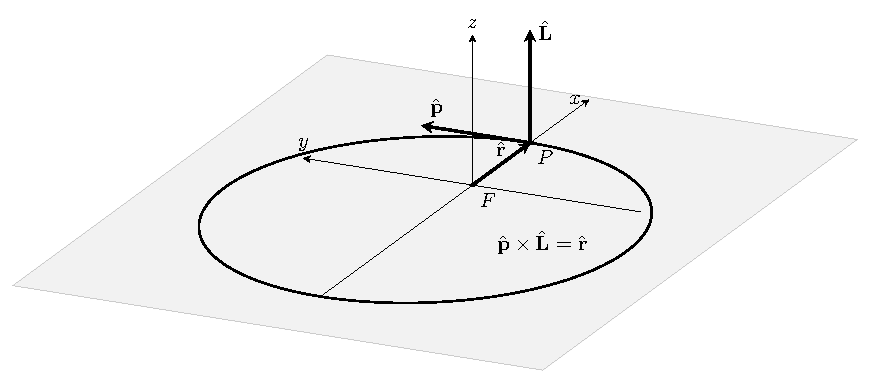
\includegraphics{fig_ch6_orbital_elements_3d.pdf}
		\caption{The Runge Lenz vector points radially outward at perigee. Since it is conserved, the direction and magnitude stays fixed during the entire evolution.}
	\end{figure}
	At periapsis the velocity is purely tangential ($\vecp\perp\rhat$), so $\rhat\times\vecA\big|_{\rm peri}=\rhat\times(\vecp\times\vecL)\big|_{\rm peri}=\big[\vecp(\rhat\cdot\vecL)-\vecL(\rhat\cdot\vecp)\big]_{\rm peri}=0$ (both dot products vanish there). Also $\rhat\cdot\vecA|_{\rm peri}=A$ (from the relation above with $v=0$ at periapsis). Together these mean $\hat A = \rhat|_{\rm peri}$: $\vecA$ points from the focus \emph{towards periapsis}.
	
	Since $\vecA$ points radially outwards at the Periapsis. We find the magnitude by doting $\vecA$ into $\vecr$:
	\begin{align}
		\vecA\cdot\vecr &= (\vecp\times\vecL)\cdot\vecr - GM\mu^2 r \\
		&=p_i L_j \epsilon_{ijk}r_k-GM\mu^2 r=p_i L_j \epsilon_{kij}r_k-GM\mu^2 r\\
		&= \underbrace{(\vecr\times\vecp)}_{\vecL}\cdot\vecL - GM\mu^2 r = L^2 - GM\mu^2 r,\end{align}
	i.e., writing $\vecA\cdot\vecr = Ar\cos v$ (with $v$ the angle between $\vecA$ and $\vecr$), using
	\[
	r = \frac{L^2/(GM\mu^2)}{1+e\cos v}\implies GM\mu^2 r = \frac{L^2}{1+e\cos v}.
	\]
	We find:
	\begin{align}
		Ar\cos v&=L^2 - GM\mu^2 r,\\
		A \frac{L^2/GM\mu^2}{1+e\cos v}\cos v&=L^2\left(1-\frac{1}{1+e\cos v}\right)=\frac{L^2e\cos v}{1+e\cos v}
	\end{align}
	
	Hence
	\begin{equation}
		\boxed{A = GM\mu^2 e.} \label{eq:A_magnitude}
	\end{equation}
	Using \eqref{eq:rhat_phihat}:
	\begin{equation}
		\hat A = \cos\omega\,\hatn+\sin\omega\,\hat y. \label{eq:Ahat}
	\end{equation}
	Equivalently, the \textbf{eccentricity vector} $\vec e \equiv \vecA/(GM\mu^2) = e\hat A=e(\cos\omega,\sin\omega,0)$ is a conserved vector encoding $(e,\omega)$ together. Since $e,\Omega,\iota$ are already determined by $(E,\vecL)$, the only \emph{new} information in $\vecA$ is $\omega$, i.e. the in-plane orientation of the ellipse or the direction of periapsis from the line of ascending node.
	
	\section{Perturbed Orbits}
	\label{sec:perturbed_orbits}
	
	We now allow an additional force $\vec F$ in the relative equation of
	motion:
	\begin{equation}
		\boxed{
			\mu\ddot{\vecr}
			=
			-\frac{GM\mu}{r^2}\rhat+\vec F .
		}
		\label{eq:perturbed_eom}
	\end{equation}
	The central Newtonian term defines the Kepler problem; $\vec F$ is the
	perturbing force and need not be central.
	
	The momentum is
	\begin{equation}
		\vecp=\mu\dot{\vecr},
	\end{equation}
	and, in the orbital plane,
	\begin{equation}
		\vecp
		=
		\mu\dot r\,\rhat+\frac{L}{r}\,\phihat,
		\qquad
		L=\mu r^2\dot\theta .
		\label{eq:polar_momentum}
	\end{equation}
	
	The purpose of orbital perturbation theory is to represent the actual
	trajectory by Keplerian orbital elements which vary with time, and to
	derive their rates directly from \eqref{eq:perturbed_eom}.
	
	\subsection{Osculating Kepler orbit}
	\label{sec:osculating_orbit}
	
	For $\vec F=0$, the Kepler solution can be written in terms of six
	constants
	\begin{equation}
		Q=(Q_1,\ldots,Q_6)
		=
		(a,e,\iota,\Omega,\omega,T_0),
	\end{equation}
	so that
	\begin{equation}
		\vecr=\vecr(Q,t),
		\qquad
		\vecp=\vecp(Q,t).
		\label{eq:kepler_phase_solution}
	\end{equation}
	For fixed $Q$, these functions satisfy the unperturbed equations of
	motion.
	
	For the perturbed problem, let
	\begin{equation}
		Q_i=Q_i(t).
	\end{equation}
	The actual trajectory is represented in terms of a set of
	time-dependent osculating orbital elements \(Q(t)\) as
	\begin{equation}
		\vecr(t)
		=
		\vecr_{\rm osc}\bigl(Q(t),t\bigr),
		\qquad
		\vecp(t)
		=
		\vecp_{\rm osc}\bigl(Q(t),t\bigr).
		\label{eq:perturbed_parameterization}
	\end{equation}
	Here, for fixed values of \(Q\), the functions
	\(\vecr_{\rm osc}(Q,t)\) and \(\vecp_{\rm osc}(Q,t)\) describe the
	corresponding Keplerian orbit.  The time dependence of \(Q(t)\) accounts
	for the slow evolution of this osculating Keplerian orbit under the
	perturbing force.
	
	At each instant, the osculating Kepler orbit is chosen to have the same
	position and momentum as the actual trajectory.  Thus,
	\begin{equation}
		\vecr_{\rm osc}\bigl(Q(t),t\bigr)=\vecr(t),
		\qquad
		\vecp_{\rm osc}\bigl(Q(t),t\bigr)=\vecp(t).
		\label{eq:osculating_state}
	\end{equation}
	Importantly, this representation does not imply that the actual
	trajectory is itself Keplerian.  Rather, it is represented at each
	instant by the Keplerian orbit that osculates it at that instant.
	
	The corresponding accelerations are different:
	\begin{align}
		\dot{\vecp}_{\rm actual}
		&=
		-\frac{GM\mu}{r^2}\rhat+\vec F,
		\\
		\dot{\vecp}_{\rm osc}
		&=
		-\frac{GM\mu}{r^2}\rhat.
	\end{align}
	Hence
	\begin{equation}
		\boxed{
			\dot{\vecp}_{\rm actual}
			-
			\dot{\vecp}_{\rm osc}
			=
			\vec F .
		}
		\label{eq:perturbation_acceleration_difference}
	\end{equation}
	
	The two trajectories therefore agree in position and momentum at the
	instant at which the osculating orbit is constructed, but they have
	different subsequent evolution.
	
	\subsection{Variation of parameters}
	
	Differentiating \eqref{eq:perturbed_parameterization},
	\begin{equation}
		\dot{\vecr}
		=
		\left.\pdv{\vecr}{t}\right|_Q
		+
		\sum_{i=1}^{6}
		\pdv{\vecr}{Q_i}\dot Q_i .
		\label{eq:r_chain_rule}
	\end{equation}
	For fixed $Q$, the first term is the velocity of the Kepler solution.
	The osculating condition requires this Kepler velocity to coincide with
	the actual velocity:
	\begin{equation}
		\dot{\vecr}
		=
		\left.\pdv{\vecr}{t}\right|_Q.
	\end{equation}
	Therefore
	\begin{equation}
		\boxed{
			\sum_{i=1}^{6}
			\pdv{\vecr}{Q_i}\dot Q_i=0 .
		}
		\label{eq:osculating_r_constraint}
	\end{equation}
	
	This is a vector equation and therefore supplies three scalar
	conditions.
	
	Now differentiate $\vecp(Q(t),t)$:
	\begin{equation}
		\dot{\vecp}
		=
		\left.\pdv{\vecp}{t}\right|_Q
		+
		\sum_{i=1}^{6}
		\pdv{\vecp}{Q_i}\dot Q_i .
		\label{eq:p_chain_rule}
	\end{equation}
	For fixed $Q$, $\vecp(Q,t)$ obeys the Kepler equation,
	\begin{equation}
		\left.\pdv{\vecp}{t}\right|_Q
		=
		-\frac{GM\mu}{r^2}\rhat .
	\end{equation}
	The actual momentum obeys
	\begin{equation}
		\dot{\vecp}
		=
		-\frac{GM\mu}{r^2}\rhat+\vec F.
	\end{equation}
	Subtracting the Kepler contribution gives
	\begin{equation}
		\boxed{
			\sum_{i=1}^{6}
			\pdv{\vecp}{Q_i}\dot Q_i
			=
			\vec F .
		}
		\label{eq:osculating_p_constraint}
	\end{equation}
	
	Equations \eqref{eq:osculating_r_constraint} and
	\eqref{eq:osculating_p_constraint} form six scalar equations for the
	six quantities $\dot Q_i$.  This is the formal variation-of-parameters
	construction of the osculating elements.
	
	The perturbing force therefore enters through the change in the
	instantaneous phase-space state; the Kepler orbit is redefined at each
	instant from that state.
	
	\subsection{Perturbed Kepler invariants}
	
	The Keplerian energy, angular momentum and eccentricity vector are
	defined from the instantaneous state by
	\begin{align}
		E
		&\equiv
		\frac{p^2}{2\mu}-\frac{GM\mu}{r},
		\label{eq:pert_E_def}
		\\
		\vec L
		&\equiv
		\vecr\times\vecp,
		\label{eq:pert_L_def}
		\\
		\vec A
		&\equiv\vecp\times\vec L-GM\mu^2\,\rhat .\label{eq:pert_A_def}
	\end{align}
	For the unperturbed Kepler problem these are constants.  In the
	perturbed problem they become time-dependent quantities.
	
	Their magnitudes determine the instantaneous Keplerian parameters:
	\begin{align}
		E&=-\frac{GM\mu}{2a(t)},
		\label{eq:instantaneous_E_a}
		\\
		L^2&=GM\mu^2a(t)(1-e^2(t)),
		\label{eq:instantaneous_L_ae}
		\\
		A&\equiv|\vec A|=GM\mu^2e(t) .
		\label{eq:instantaneous_A_e}
	\end{align}
	
	Thus $a$ and $e$ may be regarded as functions of the actual state even
	when the full trajectory is not Keplerian.
	
	\subsection{Exact Rate of the Energy}
	
	Differentiate \eqref{eq:pert_E_def}:
	\begin{align}
		\dot E
		&=
		\frac{\vecp}{\mu}\cdot\dot{\vecp}
		+
		\frac{GM\mu}{r^2}\dot r .
	\end{align}
	Using
	\begin{equation}
		\dot{\vecp}
		=
		-\frac{GM\mu}{r^2}\rhat+\vec F
	\end{equation}
	and
	\begin{equation}
		\frac{\vecp}{\mu}\cdot\rhat=\dot r,
	\end{equation}
	we obtain
	\begin{align}
		\dot E
		&=
		\dot{\vecr}\cdot
		\left(
		-\frac{GM\mu}{r^2}\rhat+\vec F
		\right)
		+
		\frac{GM\mu}{r^2}\dot r
		\\
		&=
		-\frac{GM\mu}{r^2}\dot r
		+\dot{\vecr}\cdot\vec F
		+\frac{GM\mu}{r^2}\dot r
		\\
		&=
		\boxed{
			\dot E=\dot{\vecr}\cdot\vec F .
		}
		\label{eq:perturbed_energy_rate}
	\end{align}
	
	\subsection{Exact Rate of angular momentum}
	
	From
	\begin{equation}
		\vec L=\vecr\times\vecp,
	\end{equation}
	\begin{align}
		\dot{\vec L}
		&=
		\dot{\vecr}\times\vecp
		+
		\vecr\times\dot{\vecp}.
	\end{align}
	Since $\vecp=\mu\dot{\vecr}$,
	\begin{equation}
		\dot{\vecr}\times\vecp=0,
	\end{equation}
	and hence
	\begin{align}
		\dot{\vec L}
		&=
		\vecr\times
		\left(
		-\frac{GM\mu}{r^2}\rhat+\vec F
		\right).
	\end{align}
	The central term vanishes because $\vecr\parallel\rhat$, giving
	\begin{equation}
		\boxed{
			\dot{\vec L}=\vecr\times\vec F .
		}
		\label{eq:perturbed_L_rate}
	\end{equation}
	
	Thus only the component of $\vec F$ perpendicular to $\vecr$ produces
	torque.
	
	\subsection{Exact Rate of the Runge-Lenz vector}
	
	Differentiate
	\begin{equation}
		\vec A
		=
		\vecp\times\vec L
		-
		GM\mu^2\,\rhat:
	\end{equation}
	\begin{equation}
		\dot{\vec A}
		=
		\dot{\vecp}\times\vec L
		+
		\vecp\times\dot{\vec L}
		-
		GM\mu^2\,\dot{\rhat}.
	\end{equation}
	Insert
	\begin{equation}
		\dot{\vecp}
		=
		-\frac{GM\mu}{r^2}\rhat+\vec F
	\end{equation}
	and
	\begin{equation}
		\dot{\vec L}=\vecr\times\vec F.
	\end{equation}
	Then
	\begin{align}
		\dot{\vec A}
		&=
		-\frac{GM\mu}{r^2}\rhat\times\vec L
		+
		\vec F\times\vec L
		+
		\vecp\times(\vecr\times\vec F)
		-
		GM\mu^2\,\dot{\rhat}.
	\end{align}
	
	For the Kepler part,
	\begin{equation}
		\dot{\rhat}
		=
		\frac{\vec L\times\vecr}{\mu r^3},
	\end{equation}
	so
	\begin{align}
		-GM\mu^2\,\dot{\rhat}
		&=
		-\frac{GM\mu}{r^2}\,
		\left(\vec L\times\rhat\right)
		\\
		&=
		\frac{GM\mu}{r^2}\,
		\rhat\times\vec L.
	\end{align}
	The two central terms cancel. Therefore
	\begin{equation}
		\boxed{
			\dot{\vec A}
			=
			\vec F\times\vec L
			+
			\vecp\times(\vecr\times\vec F).
		}
		\label{eq:perturbed_A_rate}
	\end{equation}
	
	This equation is the starting point for the perturbative evolution of
	the eccentricity and the orientation of periapsis.
	
	\section{Planar perturbations}
	
	We now specialize to a perturbing force confined to the orbital plane:
	\begin{equation}
		\boxed{
			\vec F
			=
			F_r\rhat+F_{\phi}\phihat .
		}
		\label{eq:planar_force}
	\end{equation}
	The angular momentum vector is perpendicular to the plane,
	\begin{equation}
		\vec L=L\hat L.
	\end{equation}
	Consequently the plane itself remains fixed:
	\begin{equation}
		\boxed{
			\dot\iota=0,
			\qquad
			\dot\Omega=0.
		}
		\label{eq:planar_plane_fixed}
	\end{equation}
	
	In the orbital plane,
	\begin{equation}
		\vecp
		=
		\mu\dot r\,\rhat+\mu r\dot\phi\,\phihat
		=
		\mu\dot r\,\rhat+\frac{L}{r}\phihat .
		\label{eq:planar_p}
	\end{equation}
	
	The equations of motion follow directly from
	\eqref{eq:perturbed_eom}:
	\begin{align}
		\mu(\ddot r-r\dot\phi^2)
		&=
		-\frac{GM\mu}{r^2}+F_r,
		\label{eq:perturbed_radial}\\
		\mu(r\ddot\phi+2\dot r\dot\phi)
		&=
		F_{\phi}.
		\label{eq:perturbed_theta}
	\end{align}
	
	The second equation gives
	\begin{equation}
		\frac{dL}{dt}
		=
		\frac{d}{dt}(\mu r^2\dot\phi)
		=
		rF_{\phi},
	\end{equation}
	so
	\begin{equation}
		\boxed{
			\dot L=rF_{\phi}.
		}
		\label{eq:planar_Ldot}
	\end{equation}
	
	The energy equation becomes
	\begin{align}
		\dot E
		&=
		\dot rF_r+r\dot\phi F_{\phi}
		\\
		&=
		\boxed{
			\dot rF_r+\frac{L}{\mu r}F_{\phi} .
		}
		\label{eq:planar_Edot}
	\end{align}
	
	\subsection{Keplerian geometry of the instantaneous ellipse}
	
	Define the true anomaly
	\begin{equation}
		f\equiv\phi-\omega .
		\label{eq:true_anomaly_def}
	\end{equation}
	For the instantaneous Kepler orbit,
	\begin{equation}
		\boxed{
			r=\frac{\lambda}{1+e\cos f},
		}
		\label{eq:instantaneous_conic}
	\end{equation}
	where
	\begin{equation}
		\boxed{
			\lambda\equiv a(1-e^2)
			=\frac{L^2}{GM\mu^2}.
		}
		\label{eq:lambda_def}
	\end{equation}
	
	The instantaneous Keplerian angular velocity is therefore
	\begin{equation}
		\dot\phi
		=
		\frac{L}{\mu r^2}.
		\label{eq:theta_dot_keplerian}
	\end{equation}
	We can obtain the instantaneous radial velocity by starting from the
	general time-dependent orbital elements,
	\begin{equation}
		a(t)=a_0+\delta a(t),\qquad
		e(t)=e_0+\delta e(t),\qquad
		\omega(t)=\omega_0+\delta\omega(t),
	\end{equation}
	where the variations $\delta a$, $\delta e$, and $\delta\omega\sim\order{\epsilon}$ are
	produced by the perturbing force. Thus, in general,
	\begin{align}
		\dot r
		=
		\pdv{r}{t}
		+
		\pdv{r}{a}\dot a
		+
		\pdv{r}{e}\dot e
		+
		\pdv{r}{f}\dot f.
	\end{align}
	For the instantaneous osculating Keplerian orbit, we take the
	zeroth-order Keplerian orbit specified by the instantaneous values of
	the orbital elements and evaluate the radial velocity with these
	elements held fixed. Equivalently, we temporarily set the
	perturbation to zero while retaining the instantaneous state
	$(\vec r,\vec p)$. Hence only the motion through the true anomaly
	contributes to the radial velocity, giving
	\begin{equation}
		\boxed{
			\dot r
			=
			\frac{dr}{df}\dot f
			=
			\frac{\lambda e\sin f}{(1+e\cos f)^2}
			\frac{L}{\mu r^2}
			=
			\frac{Le\sin f}{\mu\lambda}.
		}
		\label{eq:rdot_true_anomaly}
	\end{equation}
	
	
	Since
	\begin{equation}
		\frac{\lambda}{r}=1+e\cos f,
	\end{equation}
	we also have
	\begin{equation}
		\boxed{
			\frac{\mu r\dot r}{L}
			=
			\frac{e\sin f}{1+e\cos f}.
		}
		\label{eq:xi_relation}
	\end{equation}
	Define
	\begin{equation}
		\boxed{
			\xi\equiv
			\frac{e\sin f}{1+e\cos f}.
		}
		\label{eq:xi_def}
	\end{equation}
	
	\subsection{Rate of the semi-major axis}
	
	At a given instant, we associate the actual orbit with a Keplerian
	orbit having the same instantaneous energy. Denoting its semi-major
	axis by $a(t)$, its Keplerian energy is
	\begin{equation}
		E\bigg|_{\rm osculating}
		=
		-\frac{GM\mu}{2a},
		\qquad
		\therefore\qquad
		\dot E\bigg|_{\rm osculating}
		=
		\frac{GM\mu}{2a^2}\dot a.\label{eq:osculating_energy}
	\end{equation}
	Since the perturbing force is of order $\epsilon$,
	\[
	F_r,F_{\phi}=O(\epsilon),
	\]
	the rates of the orbital elements are themselves $O(\epsilon)$.
	Consequently, to obtain the leading, first-order evolution, the
	remaining quantities multiplying $F_r$ and $F_{\phi}$ on the
	right-hand side of \eqref{eq:planar_Edot} need only be evaluated at
	zeroth order, i.e. using the unperturbed Keplerian orbit:
	\begin{align}
		\dot{E}\bigg|_{\rm osculating}
		&=
		\left(
		\dot rF_r+\frac{L}{\mu r}F_{\phi}
		\right)_{\!0}
		\\
		&=
		\frac{L}{\mu\lambda}e\sin f\,F_r
		+
		\frac{L}{\mu r}F_{\phi}
		+O(\epsilon^2).
	\end{align}
	Hence we find:
	\begin{equation}
		\dot a
		=
		\frac{2a^2L}{GM\mu^2}
		\left[
		\frac{e\sin f}{\lambda}F_r
		+
		\frac{1}{r}F_{\phi}
		\right].
	\end{equation}
	Since
	\begin{equation}
		L=\mu\sqrt{GM\lambda},
		\qquad
		\lambda=a(1-e^2),\label{eq: angular_momenta}
	\end{equation}
	this becomes
	\begin{equation}
		\boxed{
			\dot a
			=
			\sqrt{
				\frac{4a^3}{GM\mu^2(1-e^2)}
			}
			\left[
			e\sin f\,F_r
			+
			(1+e\cos f)F_{\phi}
			\right].
		}
		\label{eq:gauss_adot}
	\end{equation}
	
	\subsection{Rate of the eccentricity}
	
	Since
	\begin{equation}
		A=GM\mu^2e,
	\end{equation}
	it is sufficient to calculate $\dot A$ from \eqref{eq:perturbed_A_rate}. For the planar perturbation, we use
	\begin{equation}
		\vec L=L\hat L
	\end{equation}
	together with
	\begin{align}
		\vec F\times\vec L
		&=
		L
		\left(
		F_r\rhat+F_{\phi}\phihat
		\right)\times\hat L
		\\
		&=
		L
		\left(
		-F_r\phihat+F_{\phi}\rhat
		\right).\\
		\vecp\times(\vecr\times\vec F)
		&=
		\left(
		\mu\dot r\rhat+\frac{L}{r}\phihat
		\right)
		\times
		\left(
		rF_{\phi}\hat L
		\right)
		\\
		&=
		L F_{\phi}\rhat-\mu r\dot r F_{\phi}\phihat .
	\end{align}
	
	Hence
	\begin{equation}
		\dot{\vec A}=
		\vec F\times\vec L
		+
		\vecp\times(\vecr\times\vec F)
		=
		2L F_{\phi}\rhat
		-
		\left(
		L F_r+\mu r\dot r F_{\phi}
		\right)\phihat .
		\label{eq:planar_Adot}
	\end{equation}
	Using \eqref{eq:xi_def},
	\begin{equation}
		\boxed{
			\dot{\vec A}
			=
			L
			\left[
			2F_{\phi}\rhat
			-
			(F_r+\xi F_{\phi})\phihat
			\right].
		}
		\label{eq:planar_Adot_xi}
	\end{equation}
	For radial perturbation $\dot{\vec{A}}=-F_rL\hat{\phi}$. The unit vector in the direction of $\vec A$ is the direction of periapsis.  Since the true anomaly is measured from periapsis,
	\begin{equation}
		\boxed{
			\hat A
			=
			\cos f\rhat-\sin f\phihat .
		}
		\label{eq:Ahat_f}
	\end{equation}
	Notice,
	\begin{align}
		\dot{\vec A} &= \dot A\hat A+A\dot{\hat A}\\
		\dot{\vec A}\cdot\hat A &=\dot A \tag{using $\dv{\hat A\cdot\hat A}{t}=0$}
	\end{align}
	Therefore
	\begin{align}
		\dot A&=\dot{\vec A}\cdot\hat A\\
		&=L\left[2F_{\phi}\cos f+(F_r+\xi F_{\phi})\sin f\right].
	\end{align}
	Thus
	\begin{equation}
		\boxed{
			\dot A
			=
			L
			\left[
			F_r\sin f
			+
			F_{\phi}
			\left(
			2\cos f+\xi\sin f
			\right)
			\right].
		}
		\label{eq:Adot_magnitude_exact}
	\end{equation}
	Up to this point, all relations have been exact. We now evaluate the exact rate equation using the instantaneous osculating Keplerian orbit, replacing the corresponding quantities on both the left- and right-hand sides by their osculating values.
	\begin{align}
		\dot A\bigg\lvert_{\rm osculating}
		&=
		L
		\left[
		F_r\sin f
		+
		F_{\phi}
		\left(
		2\cos f+\xi\sin f
		\right)
		\right]\bigg\lvert_{\rm osculating}\\
		GM\mu^2\dot e &=\sqrt{GM\mu^2 a(1-e^2)}\left[
		F_r\sin f
		+
		F_{\phi}
		\left(
		2\cos f+\xi\sin f
		\right)
		\right]
	\end{align}
	we obtain
	\begin{equation}
		\boxed{
			\dot e
			=
			\sqrt{
				\frac{a(1-e^2)}{GM\mu^2}
			}
			\left[
			F_r\sin f
			+
			F_{\phi}
			\left(
			2\cos f+\xi\sin f
			\right)
			\right].
		}
		\label{eq:gauss_edot}
	\end{equation}
	
	
	\subsection{Rate of periapsis}
	
	Define the unit vector perpendicular to $\hat A$ in the direction of
	increasing true anomaly:
	\begin{equation}
		\boxed{
			\hat q
			=
			\sin f\,\rhat+\cos f\,\phihat .
		}
		\label{eq:qhat_def}
	\end{equation}
	Differentiating \eqref{eq:Ahat_f} gives
	\begin{align}
		\dot{\hat A}
		&=
		-\dot f\sin f\,\rhat
		+\cos f\,\dot{\rhat}
		-\dot f\cos f\,\phihat
		-\sin f\,\dot{\phihat},
	\end{align}
	with
	\begin{equation}
		\dot{\rhat}=\dot\phi\,\phihat,
		\qquad
		\dot{\phihat}=-\dot\phi\,\rhat.
	\end{equation}
	Thus
	\begin{align}
		\dot{\hat A}
		&=
		(\dot\phi-\dot f)
		\left(
		\sin f\,\rhat+\cos f\,\phihat
		\right)
		\\
		&=
		\dot\omega\,\hat q,
	\end{align}
	because
	\begin{equation}
		f=\phi-\omega
		\quad\Longrightarrow\quad
		\dot f=\dot\phi-\dot\omega.
	\end{equation}
	
	Since
	\begin{equation}
		\dot{\vec A}
		=
		\dot A\,\hat A+A\dot{\hat A},
	\end{equation}
	projection onto $\hat q$ gives
	\begin{equation}
		A\dot\omega
		=
		\dot{\vec A}\cdot\hat q.
	\end{equation}
	Using \eqref{eq:planar_Adot_xi} and \eqref{eq:qhat_def},
	\begin{align}
		A\dot\omega\bigg\lvert_{\rm osculating}
		&=
		L
		\left[
		2F_{\phi}\sin f
		-
		(F_r+\xi F_{\phi})\cos f
		\right]\bigg\lvert_{\rm osculating}.
	\end{align}
	Using $A=GM\mu^2 e$, we find:
	\begin{equation}
		\boxed{
			\dot\omega
			=
			-\frac{L}{GM\mu^2e}
			\left[
			F_r\cos f
			+
			F_{\phi}
			\left(
			\xi\cos f-2\sin f
			\right)
			\right].
		}
		\label{eq:gauss_omegadot_L}
	\end{equation}
	Using
	\begin{equation}
		\frac{L}{GM\mu^2e}
		=
		\frac{1}{e}
		\sqrt{
			\frac{a(1-e^2)}{GM\mu^2}
		},
	\end{equation}
	we obtain
	\begin{equation}
		\boxed{
			\dot\omega
			=
			-\frac{1}{e}
			\sqrt{
				\frac{a(1-e^2)}{GM\mu^2}
			}
			\left[
			F_r\cos f
			+
			F_{\phi}
			\left(
			\xi\cos f-2\sin f
			\right)
			\right].
		}
		\label{eq:gauss_omegadot}
	\end{equation}
	
	\subsection{Rate of the true anomaly}
	
	Since
	\begin{equation}
		f=\phi-\omega,
	\end{equation}
	we have
	\begin{equation}
		\dot f=\dot\phi-\dot\omega.
	\end{equation}
	The instantaneous Keplerian value of $\dot\theta$ is
	\begin{equation}
		\dot\phi=\frac{L}{\mu r^2}.
	\end{equation}
	Now we apply the same osculating orbit idea and find:
	\begin{align}
		\dot f&=\frac{L}{\mu r^2}-\dot\omega\bigg\lvert_{\rm osculating}\\
		&=\sqrt{\frac{GM}{a^3}}
		\frac{(1+e\cos f)^2}{(1-e^2)^{3/2}}-\dot{\omega}\label{eq:gauss_fdot}
	\end{align}
	where we used
	\begin{equation}
		r=\frac{a(1-e^2)}{1+e\cos f}
	\end{equation}
	and
	\begin{equation}
		L=\mu\sqrt{GMa(1-e^2)}.
	\end{equation}
	
	\subsection{Planar Gauss equations}
	
	Collecting the results,
	\begin{align}
		\dot a
		&=
		\sqrt{
			\frac{4a^3}{GM\mu^2(1-e^2)}
		}
		\left[
		e\sin f\,F_r
		+
		(1+e\cos f)F_{\phi}
		\right],
		\label{eq:gauss_planar_a}
		\\[6pt]
		\dot e
		&=
		\sqrt{
			\frac{a(1-e^2)}{GM\mu^2}
		}
		\left[
		F_r\sin f
		+
		F_{\phi}
		\left(
		2\cos f+\xi\sin f
		\right)
		\right],
		\label{eq:gauss_planar_e}
		\\[6pt]
		\dot\omega
		&=
		-\frac{1}{e}
		\sqrt{
			\frac{a(1-e^2)}{GM\mu^2}
		}
		\left[
		F_r\cos f
		+
		F_{\phi}
		\left(
		\xi\cos f-2\sin f
		\right)
		\right],
		\label{eq:gauss_planar_omega}
		\\[6pt]
		\dot f
		&=
		\sqrt{\frac{GM}{a^3}}
		\frac{(1+e\cos f)^2}{(1-e^2)^{3/2}}
		-\dot\omega,
		\label{eq:gauss_planar_f}
	\end{align}
	where
	\begin{equation}
		\xi=\frac{e\sin f}{1+e\cos f}.
	\end{equation}
	For a perturbation confined to the plane,
	\begin{equation}
		\boxed{
			\dot\iota=\dot\Omega=0.
		}
	\end{equation}
	
	These equations are equations for the \emph{osculating} elements.  The
	quantities $a,e,\omega$ are therefore generally functions of time even
	though the actual position and momentum at each instant are represented
	by a Keplerian orbit.
	
	\section{Orbit-averaged evolution}
	
	The element rates above are instantaneous.  For a weak perturbation, the
	long-term evolution is obtained by inserting the unperturbed Keplerian
	orbit into the right-hand sides and averaging over one orbital period.
	
	For any quantity $X$,
	\begin{equation}
		\boxed{
			\avg{\dot X}
			=
			\frac{1}{P}\int_0^P\dot X\,dt .
		}
		\label{eq:orbit_average}
	\end{equation}
	
	For an unperturbed Kepler ellipse,
	\begin{equation}
		L=\mu r^2\dot f,
	\end{equation}
	and therefore
	\begin{equation}
		\boxed{
			dt=\frac{\mu r^2}{L}\,df.
		}
		\label{eq:dt_df}
	\end{equation}
	To first order in the perturbing force, the distinction between
	$d\theta$ and $df$ in this averaging relation produces only higher-order
	corrections.
	
	The average rate can therefore be written as
	\begin{equation}
		\avg{\dot X}
		=
		\frac{1}{P}
		\int_0^{2\pi}
		\dot X
		\frac{\mu r^2}{L}\,df .
		\label{eq:average_f}
	\end{equation}
	
	A nonzero value of $\avg{\dot X}$ represents a secular change.  Terms
	whose integral over $0\leq f\leq2\pi$ vanishes describe only short-period oscillations.
	\subsection{Example: Perturbation by an Inverse-Cube Force $F_r = \alpha/r^3$}
	
	Consider the perturbing force
	\begin{equation}
		\boxed{
			\vec F
			=
			\frac{\alpha}{r^3}\rhat .
		}
		\label{eq:worked_force}
	\end{equation}
	Thus
	\begin{equation}
		F_r=\frac{\alpha}{r^3},
		\qquad
		F_{\phi}=0.
	\end{equation}
	
	%----------------------------------------------------------
	\subsubsection{Rate of the semimajor axis}
	
	Differentiating \eqref{eq:osculating_energy}, we obtain
	\begin{equation}
		\dot E
		=
		\frac{GM\mu}{2a^2}\dot a.
		\label{eq:energy_a}
	\end{equation}
	
	The exact rate of change of the energy of the actual orbit is
	\begin{equation}
		\dot E
		=
		\vec F\cdot\vec v.
		\label{eq:energy_rate}
	\end{equation}
	
	Since the perturbation is radial,
	\begin{equation}
		\vec F
		=
		\frac{\alpha}{r^3}\rhat,\qquad
		\vec v
		=
		\dot r\,\rhat
		+
		r\dot f\,\phihat,
	\end{equation}
	we have
	\begin{equation}
		\dot E
		=
		\frac{\alpha}{r^3}\dot r.
		\label{eq:energy_radial}
	\end{equation}
	
	For the osculating Keplerian orbit, from \eqref{eq:rdot_true_anomaly} with $\lambda=\frac{L^2}{GM\mu^2}$,
	\begin{equation}
		\dot r
		=
		\frac{GM\mu}{L}e\sin f.
		\label{eq:osculating_rdot}
	\end{equation}
	
	Therefore,
	\begin{equation}
		\dot E
		=
		\frac{\alpha GM\mu}{Lr^3}e\sin f.
	\end{equation}
	
	Comparing this result with \eqref{eq:energy_a},
	\begin{equation}
		\frac{GM\mu}{2a^2}\dot a
		=
		\frac{\alpha GM\mu}{Lr^3}e\sin f,
	\end{equation}
	so that
	\begin{equation}
		\boxed{
			\dot a
			=
			\frac{2\alpha a^2e\sin f}{Lr^3}
		}.
		\label{eq:adot}
	\end{equation}
	
	
	%----------------------------------------------------------
	\subsubsection{Rate of the eccentricity}
	
	Define the eccentricity vector by
	\begin{equation}
		\vec A
		=
		\vecp\times\vec L
		-
		GM\mu^2\rhat.
		\label{eq:A_definition}
	\end{equation}
	
	For the osculating Keplerian orbit,
	\begin{equation}
		A
		=
		GM\mu^2 e.
		\label{eq:A_e}
	\end{equation}
	
	Since the perturbing force is radial,
	\begin{equation}
		\dot{\vec L}
		=
		\vecr\times\vec F
		=
		\vecr\times
		\frac{\alpha}{r^3}\rhat
		=
		0.
		\label{eq:Ldot_zero}
	\end{equation}
	
	Differentiating $L^2=GM\mu^2a(1-e^2),$	gives
	\begin{equation}
		2L\dot L
		=
		GM\mu^2
		\left[
		(1-e^2)\dot a
		-
		2ae\dot e
		\right].
	\end{equation}

	Therefore,
	\begin{equation}
		\dot e
		=
		\frac{1-e^2}{2ae}\dot a
		\label{eq:edot_adot}
	\end{equation}
	
	Substituting \eqref{eq:adot},
	\begin{equation}
		\dot e
		=
		\frac{1-e^2}{2ae}
		\frac{2\alpha a^2e\sin f}{Lr^3}=
		\frac{1-e^2}{2ae}
		\frac{2\alpha a^2e\sin f}{Lr^3}.
	\end{equation}

	
	%----------------------------------------------------------
	\subsubsection{Rate of the argument of periapsis}
	
	We now determine the rate of the direction of the eccentricity
	vector.	Differentiating \eqref{eq:A_definition},
	\begin{equation}
		\dot{\vec A}
		=
		\dot{\vecp}\times\vec L
		+
		\vecp\times\dot{\vec L}
		-
		GM\mu^2\dot{\rhat}.
	\end{equation}
	
	Since $\dot{\vec L}=0$,
	\begin{equation}
		\dot{\vec A}
		=
		\dot{\vecp}\times\vec L
		-
		GM\mu^2\dot{\rhat}.
	\end{equation}
	
	The momentum equation is
	\begin{equation}
		\dot{\vecp}
		=
		-\frac{GM\mu}{r^2}\rhat
		+
		\frac{\alpha}{r^3}\rhat.
	\end{equation}
	
	Therefore,
	\begin{equation}
		\dot{\vec A}
		=
		\left(
		-\frac{GM\mu}{r^2}
		+
		\frac{\alpha}{r^3}
		\right)
		\underbrace{\rhat\times\vec L}_{\mathclap{=-L\phihat}}
		-
		\underbrace{GM\mu^2\underbrace{\dot{\rhat}}_{\mathclap{=\dot f\,\phihat}}}_{=\frac{GM\mu L}{r^2}\phihat}.
	\end{equation}
	Consequently, the terms containing the central gravitational
	force cancel, leaving
	\begin{equation}
		\dot{\vec A}
		=
		-\frac{\alpha L}{r^3}\phihat.
		\label{eq:Adot}
	\end{equation}
	
	Let $\hat{\boldsymbol e}$ be the unit vector pointing toward
	periapsis and let $\hat{\boldsymbol e}_{\perp}$ be the unit vector
	obtained by rotating $\hat{\boldsymbol e}$ by $90^\circ$ in the
	direction of increasing true anomaly. Then, from \eqref{eq:Ahat_f}
	\begin{equation}
		\vec A
		=
		A\hat{\boldsymbol e},\qquad \hat{\boldsymbol e}=\cos\omega\hatn+\sin\omega\hat y,
	\end{equation}
	and therefore
	\begin{equation}
		\dot{\vec A}
		=
		\dot A\,\hat{\boldsymbol e}
		+
		A\dot\omega\,\hat{\boldsymbol e}_{\perp}.
		\label{eq:Adot_decomposition}
	\end{equation}
	
	The radial and transverse unit vectors are related to the periapsis
	basis by
	\begin{equation}
		\rhat
		=
		\cos f\,\hat{\boldsymbol e}
		+
		\sin f\,\hat{\boldsymbol e}_{\perp},
	\end{equation}
	and
	\begin{equation}
		\phihat
		=
		-\sin f\,\hat{\boldsymbol e}
		+
		\cos f\,\hat{\boldsymbol e}_{\perp}.
	\end{equation}
	
	Substituting the latter relation into \eqref{eq:Adot},
	\begin{equation}
		\dot{\vec A}
		=
		-\frac{\alpha L}{r^3}
		\left(
		-\sin f\,\hat{\boldsymbol e}
		+
		\cos f\,\hat{\boldsymbol e}_{\perp}
		\right).
	\end{equation}
	
	Hence,
	\begin{equation}
		\dot{\vec A}
		=
		\frac{\alpha L}{r^3}\sin f\,\hat{\boldsymbol e}
		-
		\frac{\alpha L}{r^3}\cos f\,
		\hat{\boldsymbol e}_{\perp}.
	\end{equation}
	
	Comparing this with \eqref{eq:Adot_decomposition}, we obtain
	\begin{equation}
		\dot A
		=
		\frac{\alpha L}{r^3}\sin f,
		\label{eq:Adot_magnitude_radial_pert}
	\end{equation}
	and
	\begin{equation}
		A\dot\omega
		=
		-\frac{\alpha L}{r^3}\cos f.
	\end{equation}
	
	Using
	\begin{equation}
		A=GM\mu^2e,
	\end{equation}
	we finally obtain
	\begin{equation}
		\boxed{
			\dot\omega
			=
			-\frac{\alpha L}{GM\mu^2e\,r^3}\cos f
		}.
		\label{eq:omegadot}
	\end{equation}
	
	\subsection{Semi-major axis}
	
	Equation \eqref{eq:gauss_planar_a} gives
	\begin{equation}
		\dot a
		=
		\sqrt{
			\frac{4a^3}{GM\mu^2(1-e^2)}
		}
		\,e\sin f\,
		\frac{\alpha}{r^3}.
	\end{equation}
	Hence
	\begin{equation}
		\boxed{
			\dot a
			=
			\frac{2\alpha a^2}{GM\mu r^3}\dot r .
		}
		\label{eq:worked_adot}
	\end{equation}
	
	For the Keplerian ellipse introduce the eccentric anomaly $u$:
	\begin{equation}
		r=a(1-e\cos u),
	\end{equation}
	and
	\begin{equation}
		\dot r
		=
		\frac{ane\sin u}{1-e\cos u},
		\qquad
		n=\sqrt{\frac{GM}{a^3}}.
	\end{equation}
	Therefore
	\begin{equation}
		\boxed{
			\dot a
			=
			\frac{
				2\alpha e n\sin u
			}{
				GM\mu(1-e\cos u)^4
			}.
		}
		\label{eq:worked_adot_u}
	\end{equation}
	
	Over one unperturbed orbit,
	\begin{equation}
		dt
		=
		\frac{1-e\cos u}{n}\,du,
	\end{equation}
	so
	\begin{align}
		\Delta a
		&=
		\int_0^{2\pi}\dot a\,dt
		\\
		&=
		\frac{2\alpha e}{GM\mu}
		\int_0^{2\pi}
		\frac{\sin u}{(1-e\cos u)^3}\,du
		\\
		&=0 .
	\end{align}
	Thus
	\begin{equation}
		\boxed{
			\avg{\dot a}=0
		}
		\label{eq:worked_a_secular}
	\end{equation}
	to first order in the perturbation.
	
	The osculating semi-major axis therefore oscillates during an orbit but
	has no secular drift.
	
	\subsection{Eccentricity}
	
	From angular-momentum conservation,
	\begin{equation}
		L^2=GM\mu^2a(1-e^2)
	\end{equation}
	and therefore
	\begin{equation}
		0
		=
		(1-e^2)\dot a
		-
		2ae\dot e .
	\end{equation}
	Hence
	\begin{equation}
		\boxed{
			\dot e
			=
			\frac{1-e^2}{2ae}\dot a .
		}
		\label{eq:worked_edot_relation}
	\end{equation}
	Since $\avg{\dot a}=0$,
	\begin{equation}
		\boxed{
			\avg{\dot e}=0 .
		}
		\label{eq:worked_e_secular}
	\end{equation}
	
	\subsection{Apsidal precession}
	
	For the radial force, \eqref{eq:gauss_planar_omega} reduces to
	\begin{equation}
		\boxed{
			\dot\omega
			=
			-\frac{\alpha L\cos f}
			{GM\mu^2e\,r^3}.
		}
		\label{eq:worked_omega_dot}
	\end{equation}
	
	To first order in $\alpha$, evaluate the secular change using the
	unperturbed Keplerian relation
	\begin{equation}
		r=\frac{\lambda}{1+e\cos f},
		\qquad
		\lambda=a(1-e^2),
	\end{equation}
	together with
	\begin{equation}
		dt=\frac{\mu r^2}{L}\,df.
	\end{equation}
	Then
	\begin{align}
		\Delta\omega
		&=
		\int_0^{2\pi}\dot\omega\,dt
		\\
		&=
		-\frac{\alpha}{GM\mu e}
		\int_0^{2\pi}
		\frac{\cos f}{r}\,df
		\\
		&=
		-\frac{\alpha}{GM\mu e}
		\int_0^{2\pi}
		\frac{1+e\cos f}{\lambda}\cos f\,df
		\\
		&=
		-\frac{\alpha}{GM\mu e\lambda}
		\left[
		\int_0^{2\pi}\cos f\,df
		+
		e\int_0^{2\pi}\cos^2f\,df
		\right].
	\end{align}
	Since
	\begin{equation}
		\int_0^{2\pi}\cos f\,df=0,
		\qquad
		\int_0^{2\pi}\cos^2f\,df=\pi,
	\end{equation}
	we obtain
	\begin{equation}
		\boxed{
			\Delta\omega
			=
			-\frac{\pi\alpha}
			{GM\mu\,a(1-e^2)} .
		}
		\label{eq:worked_precession_per_orbit}
	\end{equation}
	
	Using
	\begin{equation}
		P=2\pi\sqrt{\frac{a^3}{GM}},
	\end{equation}
	the secular rate is
	\begin{equation}
		\boxed{
			\avg{\dot\omega}
			=
			-\frac{\alpha}{2\mu\sqrt{GM}\,a^{5/2}(1-e^2)} .	}
		\label{eq:worked_precession_rate}
	\end{equation}
	
	The same result follows directly from the exact Binet equation for the
	full force
	\begin{equation}
		F_r=-\frac{GM\mu}{r^2}+\frac{\alpha}{r^3}.
	\end{equation}
	Writing $u=1/r$ gives
	\begin{equation}
		u''+
		\left(
		1+\frac{\alpha\mu}{L^2}
		\right)u
		=
		\frac{GM\mu^2}{L^2},
	\end{equation}
	where primes denote derivatives with respect to $\theta$.  Hence the
	radial oscillation has angular frequency
	\begin{equation}
		\kappa
		=
		\sqrt{
			1+\frac{\alpha\mu}{L^2}
		},
	\end{equation}
	and the apsidal angle is
	\begin{equation}
		\Delta\theta_{\rm apsis}
		=
		\frac{2\pi}{\kappa}.
	\end{equation}
	The exact apsidal shift relative to $2\pi$ is therefore
	\begin{equation}
		\Delta\omega_{\rm exact}
		=
		2\pi
		\left[
		\frac{1}{
			\sqrt{1+\alpha\mu/L^2}
		}
		-1
		\right].
	\end{equation}
	For a weak perturbation,
	\begin{equation}
		\frac{\alpha\mu}{L^2}\ll1,
	\end{equation}
	so
	\begin{align}
		\Delta\omega_{\rm exact}
		&=
		-\frac{\pi\alpha\mu}{L^2}
		+O(\alpha^2)
		\\
		&=
		-\frac{\pi\alpha}
		{GM\mu\,a(1-e^2)}
		+O(\alpha^2),
	\end{align}
	which agrees with the orbit-averaged planetary equation.
	\section{Nearly circular orbits}
	\label{sec:nearly_circular}
	
	As $e\rightarrow0$, the argument of periapsis becomes undefined:
	a circle has no distinguished periapsis.  The explicit $1/e$ in
	\eqref{eq:gauss_planar_omega} is therefore a coordinate singularity.
	
	Instead of $(e,\omega)$, use the two Cartesian components of the
	eccentricity vector:
	\begin{equation}
		\boxed{
			\epsilon_1=e\cos\omega,
			\qquad
			\epsilon_2=e\sin\omega.
		}
		\label{eq:LL_vars}
	\end{equation}
	
	For small $e$, define
	\begin{equation}
		\Phi\equiv\theta\big|_{e=0} ,
	\end{equation}
	and write
	\begin{equation}
		\theta
		=
		\Phi
		+
		2\epsilon_1\sin\Phi
		-
		2\epsilon_2\cos\Phi
		+O(e^2).
		\label{eq:small_e_theta}
	\end{equation}
	Using
	\begin{equation}
		r=\frac{a(1-e^2)}{1+e\cos(\theta-\omega)}
	\end{equation}
	and retaining terms through first order in
	$\epsilon_1,\epsilon_2$ gives
	\begin{equation}
		\boxed{
			r
			=
			a
			\left(
			1-\epsilon_1\cos\Phi-\epsilon_2\sin\Phi
			\right)
			+O(e^2).
		}
		\label{eq:small_e_r}
	\end{equation}
	
	Differentiating,
	\begin{equation}
		\dot r
		=
		an
		\left(
		\epsilon_1\sin\Phi-\epsilon_2\cos\Phi
		\right)
		+O(e^2),
	\end{equation}
	where
	\begin{equation}
		n=\sqrt{\frac{GM}{a^3}}.
	\end{equation}
	Also,
	\begin{equation}
		\boxed{
			\dot\theta
			=
			n
			\left(
			1+2\epsilon_1\cos\Phi
			+2\epsilon_2\sin\Phi
			\right)
			+O(e^2).
		}
		\label{eq:small_e_theta_dot}
	\end{equation}
	
	Define
	\begin{equation}
		\delta\theta
		\equiv
		\theta-\Phi
		=
		2\epsilon_1\sin\Phi
		-
		2\epsilon_2\cos\Phi .
	\end{equation}
	
	The nonsingular variables $\epsilon_1,\epsilon_2$ are preferable to
	$\omega$ near circularity because they remain finite as $e\to0$.
	
	\subsection{First-order equations for nearly circular motion}
	
	Substituting the small-$e$ parameterization into the energy equation gives
	\begin{equation}
		\boxed{
			\dot a
			=
			\sqrt{\frac{4a^3}{GM\mu^2}}
			\left[
			\delta\theta\,F_r
			+
			\left(
			1+\epsilon_1\cos\Phi+\epsilon_2\sin\Phi
			\right)F_{\phi}
			\right]
			+O(e^2F).
		}
		\label{eq:LL_adot}
	\end{equation}
	
	The eccentricity vector is
	\begin{equation}
		\vec A
		=
		GM\mu^2
		\left(
		\epsilon_1\hatn+\epsilon_2\hat y
		\right)
		+O(e^2),
	\end{equation}
	and its evolution gives
	\begin{align}
		\boxed{
			\dot\epsilon_1
			=
			\sqrt{\frac{a}{GM\mu^2}}
			\left[
			\sin\Phi\,F_r
			+
			2\cos\Phi\,F_{\phi}
			+
			\delta\theta
			\left(
			2\cos\Phi\,F_r-3\sin\Phi\,F_{\phi}
			\right)
			\right]
			+O(e^2F),
		}
		\label{eq:LL_eps1dot}
		\\[6pt]
		\boxed{
			\dot\epsilon_2
			=
			\sqrt{\frac{a}{GM\mu^2}}
			\left[
			-\cos\Phi\,F_r
			+
			2\sin\Phi\,F_{\phi}
			+
			\delta\theta
			\left(
			2\sin\Phi\,F_r+3\cos\Phi\,F_{\phi}
			\right)
			\right]
			+O(e^2F).
		}
		\label{eq:LL_eps2dot}
	\end{align}
	
	To zeroth order in $e$,
	\begin{equation}
		\boxed{
			\dot\Phi=n+O(e^2).
		}
		\label{eq:LL_Phi_dot}
	\end{equation}
	
	Using $\Phi$ as the independent variable,
	\begin{align}
		\boxed{
			\frac{da}{d\Phi}
			=
			\frac{2a^3}{GM\mu}
			\left[
			\delta\theta\,F_r
			+
			\left(
			1+\epsilon_1\cos\Phi+\epsilon_2\sin\Phi
			\right)F_{\phi}
			\right],
		}
		\label{eq:LL_dadPhi}
		\\
		\boxed{
			\frac{d\epsilon_1}{d\Phi}
			=
			\frac{a^2}{GM\mu}
			\left[
			\sin\Phi\,F_r
			+
			2\cos\Phi\,F_{\phi}
			+
			\delta\theta
			\left(
			2\cos\Phi\,F_r-3\sin\Phi\,F_{\phi}
			\right)
			\right],
		}
		\label{eq:LL_deps1dPhi}
		\\
		\boxed{
			\frac{d\epsilon_2}{d\Phi}
			=
			\frac{a^2}{GM\mu}
			\left[
			-\cos\Phi\,F_r
			+
			2\sin\Phi\,F_{\phi}
			+
			\delta\theta
			\left(
			2\sin\Phi\,F_r+3\cos\Phi\,F_{\phi}
			\right)
			\right].
		}
		\label{eq:LL_deps2dPhi}
	\end{align}
	
	
	
	\section{Rømer delay for a Keplerian binary}
	\label{sec:romer}
	
	For a binary of component masses $m_1$ and $m_2$,
	\begin{equation}
		M=m_1+m_2.
	\end{equation}
	Let $\vecr$ be the relative separation and let the primary's
	barycentric position be
	\begin{equation}
		\vecx_1
		=
		\frac{m_2}{M}\vecr .
	\end{equation}
	
	If $\hat R$ points from the source towards the observer, the
	light-travel-time contribution is
	\begin{equation}
		\Delta_R
		=
		-\frac{\vecx_1\cdot\hat R}{c}.
	\end{equation}
	
	Using the orbital-plane basis,
	\begin{equation}
		\vecr
		=
		r
		\left[
		\cos\theta\,\hatn+\sin\theta\,\hat y
		\right],
	\end{equation}
	with
	\begin{equation}
		\theta=\omega+f,
	\end{equation}
	and
	\begin{equation}
		\hat y\cdot\hat R=\sin\iota,
		\qquad
		\hatn\cdot\hat R=0,
	\end{equation}
	we obtain
	\begin{equation}
		\Delta_R
		=
		\frac{m_2}{Mc}\,
		r\sin\iota\,\sin(\omega+f).
	\end{equation}
	
	Define
	\begin{equation}
		a_1=\frac{m_2}{M}a,
	\end{equation}
	and use the eccentric-anomaly relations
	\begin{align}
		r\cos f
		&=
		a(\cos u-e),
		\\
		r\sin f
		&=
		a\sqrt{1-e^2}\sin u.
	\end{align}
	Since
	\begin{equation}
		\sin(\omega+f)
		=
		\sin\omega\cos f+\cos\omega\sin f,
	\end{equation}
	we obtain
	\begin{equation}
		\boxed{
			\Delta_R
			=
			\frac{a_1\sin\iota}{c}
			\left[
			(\cos u-e)\sin\omega
			+
			\sqrt{1-e^2}\sin u\cos\omega
			\right].
		}
		\label{eq:romer_delay}
	\end{equation}

\section{Applied Orbital Mechanics: Binary Stars, Transfer Orbits, and Perturbations}

This section brings together the theoretical framework of two-body dynamics through eleven comprehensive worked problems covering binary star astrometry, spectroscopic radial-velocity mass determination, symmetric mass ratios, numerical solution of Kepler's equation, orbital transfers, conserved vectors, continuous thrust perturbation theory, dynamical mass estimation for extended (halo-scale) systems, and the line-of-sight projection connecting an orbit's orientation in space to what an observer actually measures.

\subsection{Problem 1: Astrometric Binary White Dwarf System}

\textbf{Problem Statement}: Two white dwarfs in a binary system appear on the sky plane as concentric circles of radii $1\,\mu\text{as}$ and $0.5\,\mu\text{as}$, respectively, moving anticlockwise. The observed orbital period is $1\,\text{day}$. The system has a parallax of $1\,\text{mas}$.
\begin{enumerate}[label=(\alph*)]
	\item What is the semi-major axis of the relative orbit?
	\item The stars appear to move with constant angular speed along circular trajectories. What are the orbital eccentricity $e$ and inclination $i$?
	\item Find the individual masses $m_1$ and $m_2$ and the total mass $M$.
	\item If the orbit were inclined, what would be the orientation of the orbit in space? Specify the angles $\Omega$ and $\omega$.
	\item What is the magnitude of the Runge--Lenz vector for this system?
\end{enumerate}

\textbf{Essential Ideas}:
\begin{itemize}
	\item \textbf{Center of mass}: For a binary system, both stars orbit their mutual center of mass with identical period $T$. Their individual barycentric semi-major axes satisfy
	\[
	a=a_1+a_2, \qquad m_1a_1=m_2a_2,
	\]
	where $a$ is the semi-major axis of the relative orbit.
	
	\begin{figure}[htbp]
		\centering
		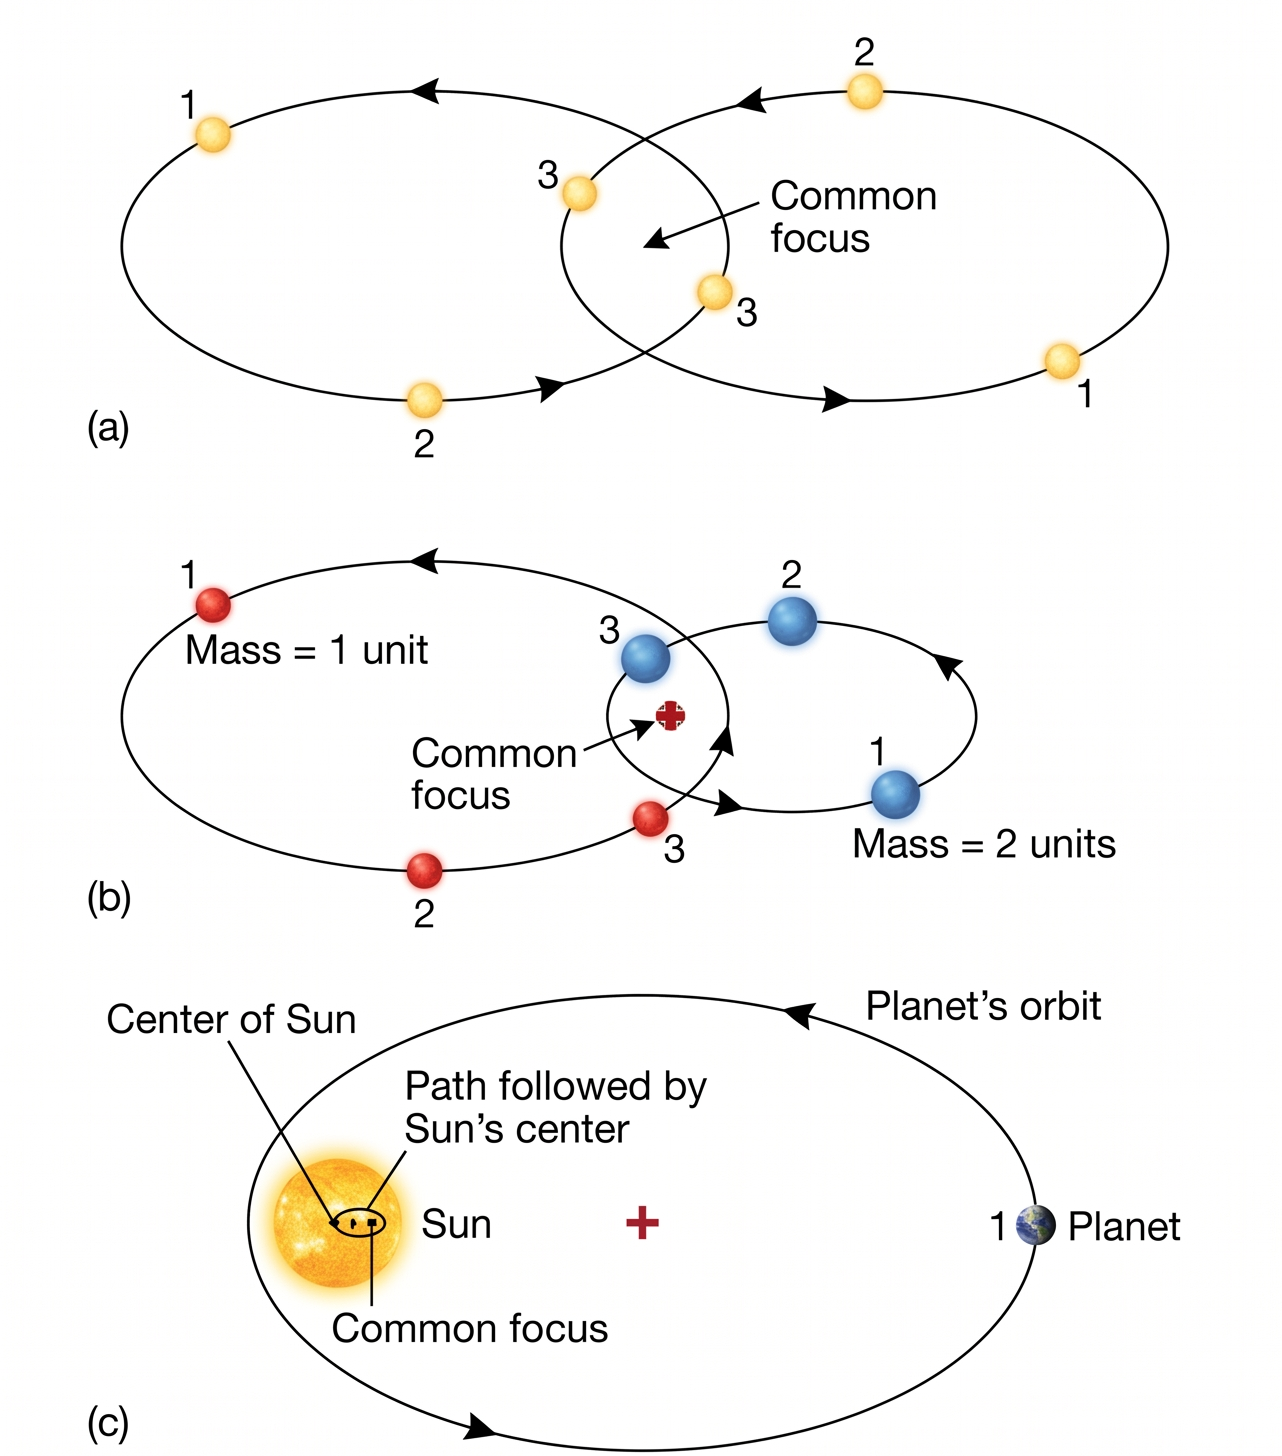
\includegraphics[width=0.7\linewidth]{Two Body Problem.png}
		\caption{Both stars orbit the common center of mass. Their position vectors are scaled, oppositely directed copies of the relative separation vector, $\vec r_1=(m_2/M)\vec r$ and $\vec r_2=-(m_1/M)\vec r$.}
		\label{fig:two-body-problem}
	\end{figure}
	
	\item \textbf{Projected orbit}: A circular orbit tilted with respect to the sky plane projects to an ellipse. Therefore an observed circle requires $i=0^\circ$. Constant orbital speed then implies a circular Kepler orbit, so $e=0$.
	
	\item \textbf{Runge--Lenz vector}: The Runge--Lenz vector points towards the periapsis with magnitude
	\[
	|\vec A| = GM\mu^2 e.
	\]
	For a circular orbit ($e=0$), $\vec A = \vec 0$.
\end{itemize}

\textbf{Detailed Solutions}:
\begin{enumerate}[label=(\alph*)]
	\item \textbf{Semi-major axis of the relative orbit:}
	
	The distance $d$ to the binary follows from the parallax $\varpi = 1\,\text{mas} = 10^{-3\,\prime\prime}$:
	\[
	d = \frac{1\,\mathrm{AU}}{\varpi} = \frac{1\,\mathrm{AU}}{10^{-3\,\prime\prime}} = 10^3\,\mathrm{pc}.
	\]
	The physical barycentric orbital radii are
	\begin{align*}
		a_1 &= \theta_1 d = (1\,\mu\text{as})(10^3\,\text{pc}) = (10^{-6\,\prime\prime})(10^3\,\text{pc}) = 10^{-3}\,\mathrm{AU} \simeq 1.496 \times 10^8\,\mathrm{m}, \\
		a_2 &= \theta_2 d = (0.5\,\mu\text{as})(10^3\,\text{pc}) = (0.5 \times 10^{-6\,\prime\prime})(10^3\,\text{pc}) = 0.5 \times 10^{-3}\,\mathrm{AU} \simeq 7.48 \times 10^7\,\mathrm{m}.
	\end{align*}
	Therefore, the relative separation has semi-major axis:
	\[
	\boxed{a = a_1 + a_2 = 1.5 \times 10^{-3}\,\mathrm{AU} = 2.244 \times 10^8\,\mathrm{m}}.
	\]
	
	\begin{figure}[htbp]
		\centering
		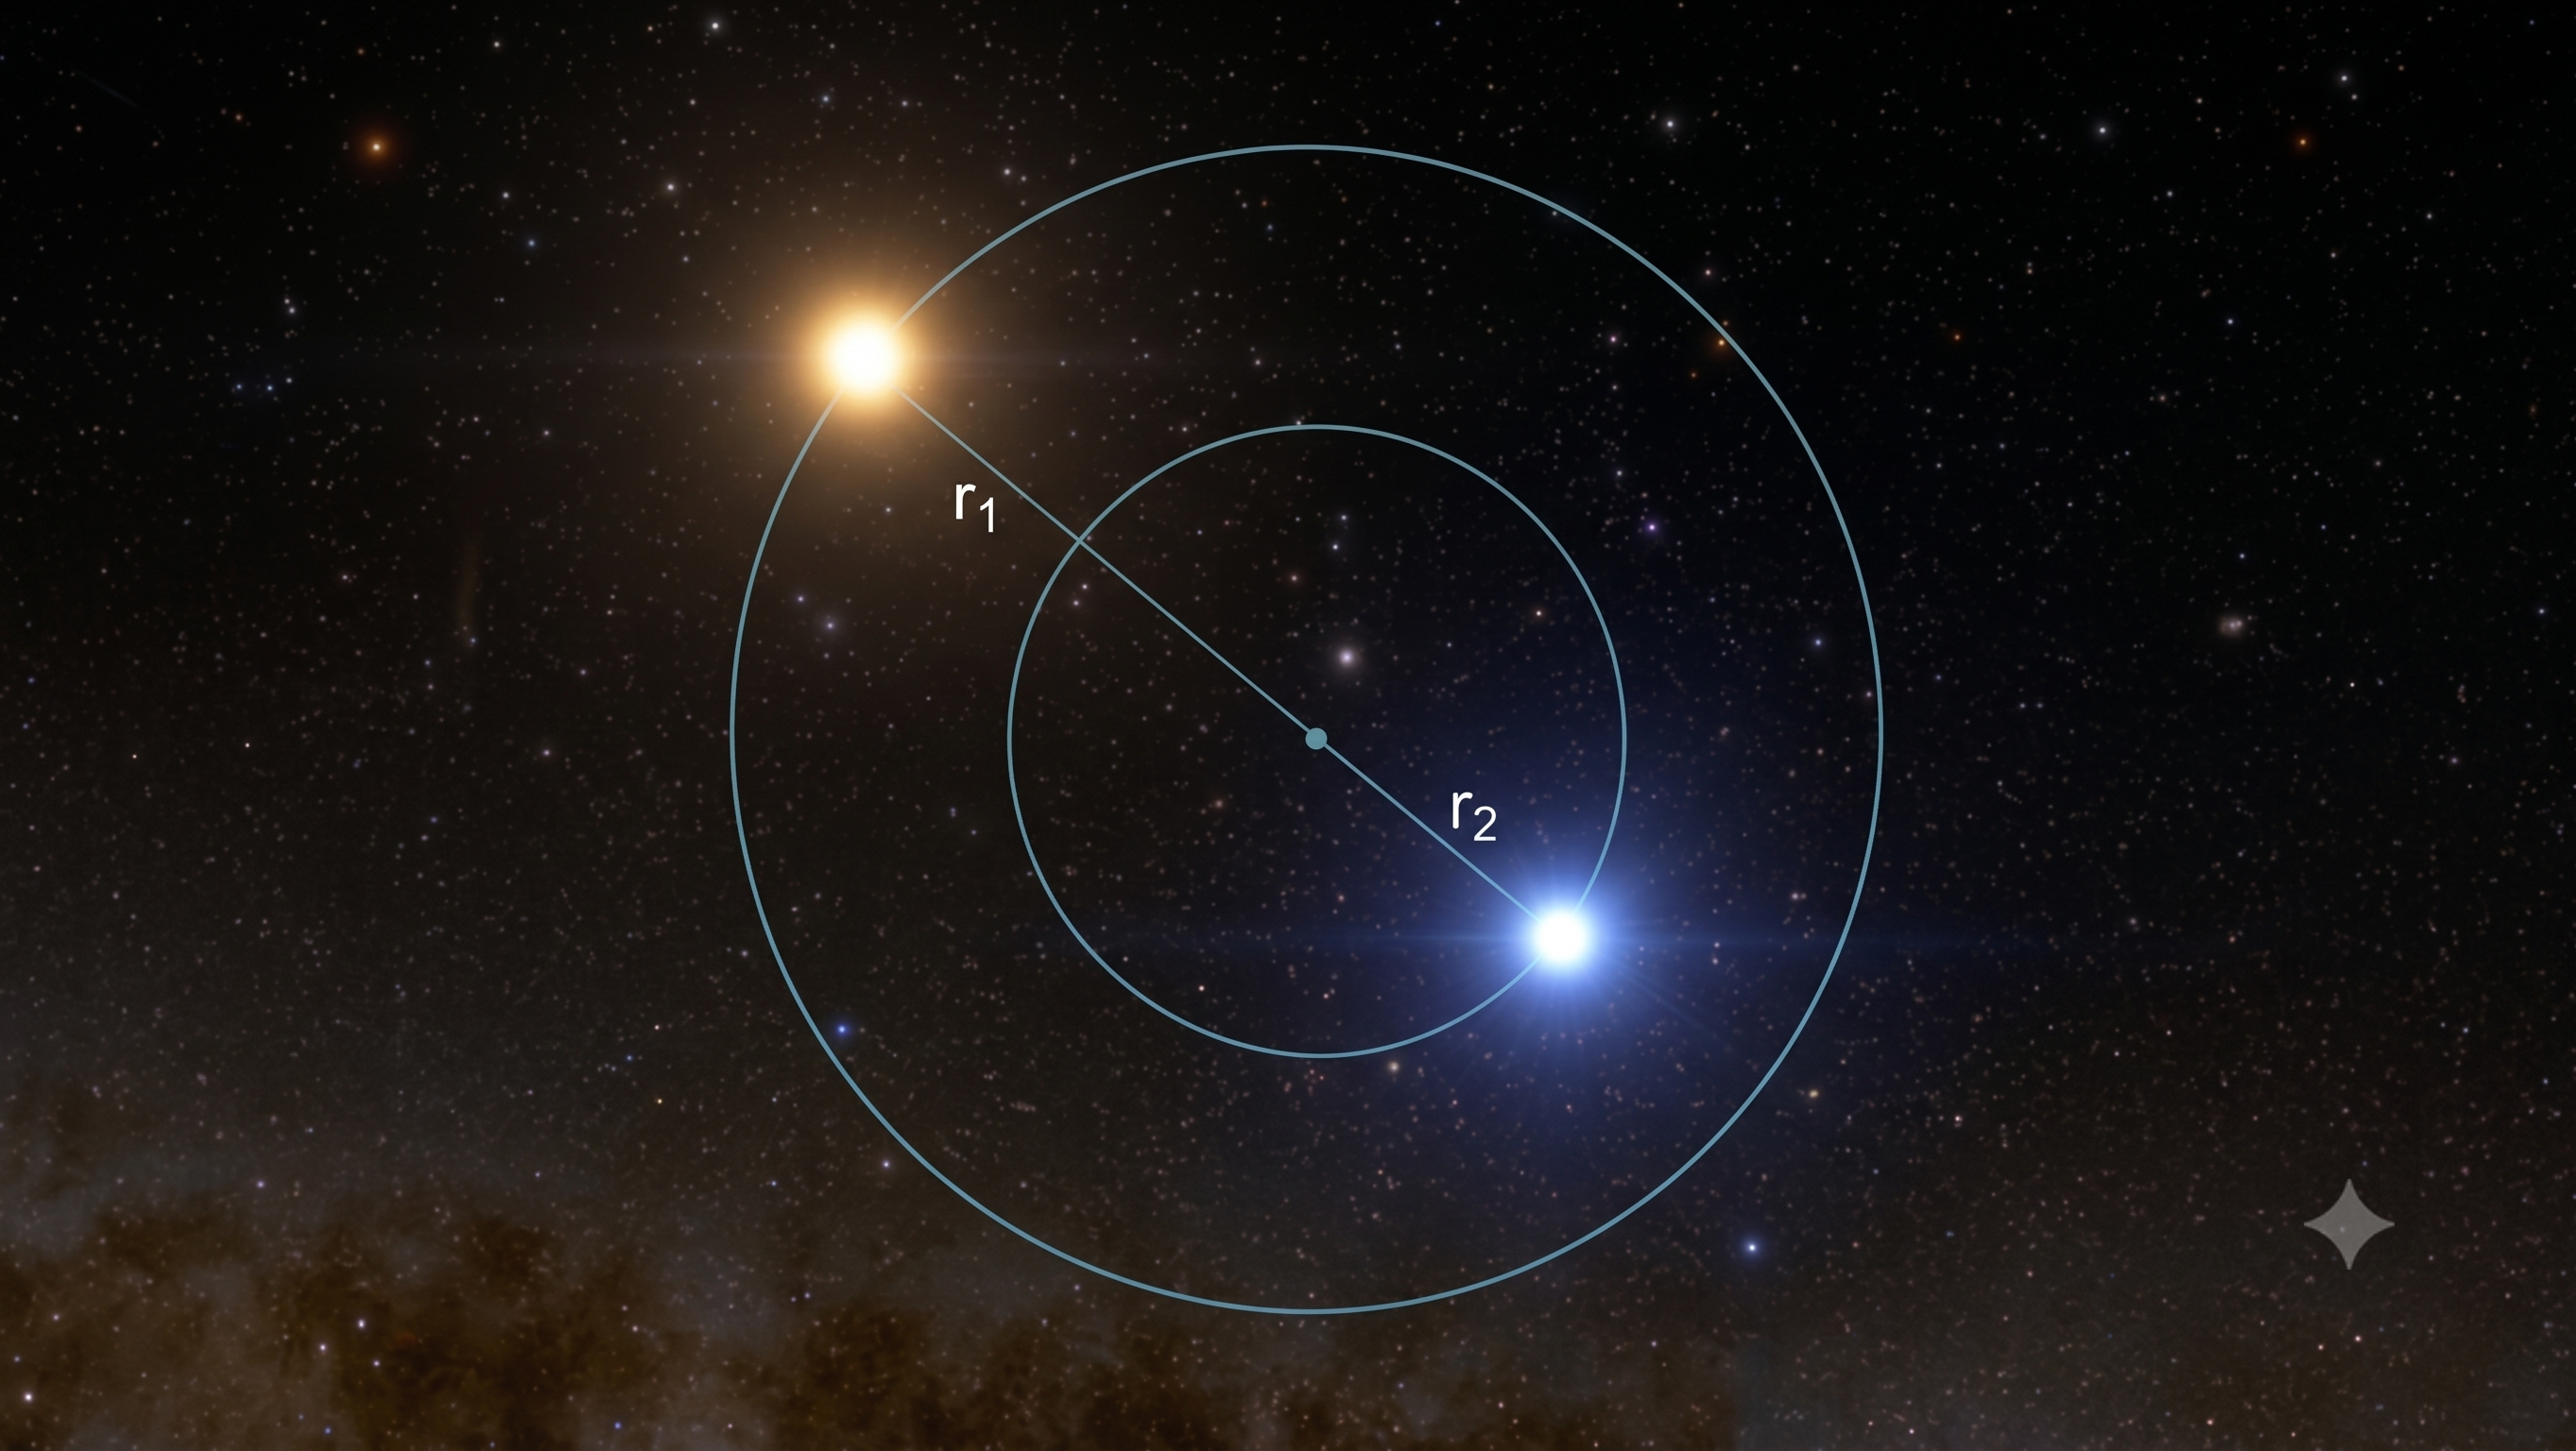
\includegraphics[width=0.7\linewidth]{Binary_Star.png}
		\caption{The two barycentric orbital radii add to give the instantaneous relative separation. Consequently their semi-major axes satisfy $a=a_1+a_2$.}
		\label{fig:binarystar}
	\end{figure}
	
	\item \textbf{Eccentricity and inclination:}
	
	Since the observed trajectories are circles, the projection factor satisfies $\cos i = 1 \implies \boxed{i = 0^\circ}$. Since the orbital speed is constant, the orbit is circular: $\boxed{e = 0}$.
	
	\item \textbf{Masses:}
	
	The mass ratio is inversely proportional to the barycentric semi-major axes:
	\[
	\frac{m_1}{m_2} = \frac{a_2}{a_1} = \frac{0.5}{1.0} = \frac{1}{2} \implies m_2 = 2m_1.
	\]
	From Kepler's third law:
	\[
	T^2 = \frac{4\pi^2 a^3}{G(m_1+m_2)} = \frac{4\pi^2 a^3}{3Gm_1}.
	\]
	With $T = 1\,\text{day} = 86400\,\text{s}$ and $a = 2.244 \times 10^8\,\mathrm{m}$:
	\[
	M = m_1 + m_2 = \frac{4\pi^2 a^3}{G T^2} \simeq 8.91 \times 10^{29}\,\mathrm{kg} \simeq 0.448\,M_\odot.
	\]
	Thus:
	\[
	\boxed{m_1 \simeq 0.149\,M_\odot}, \qquad \boxed{m_2 \simeq 0.299\,M_\odot}.
	\]
	
	\item \textbf{Orientation angles $\Omega$ and $\omega$:}
	
	For a circular face-on orbit ($i=0^\circ, e=0$), the line of nodes is undefined (no intersection between orbital and sky planes), and the periapsis is undefined (distance is constant). Hence neither $\Omega$ nor $\omega$ is uniquely defined.
	
	\item \textbf{Runge--Lenz Vector:}
	
	Because the orbit is circular ($e=0$), $\vec A = \vec 0$. For a circular orbit there is no distinguished periapsis direction, which is exactly why the Runge--Lenz vector vanishes.
\end{enumerate}

\subsection{Problem 2: Bounds on the Symmetric Mass Ratio}

\textbf{Problem Statement}: Prove that the symmetric mass ratio $\eta = \frac{m_1m_2}{M^2}$ (where $M = m_1+m_2$) satisfies $\eta \in (0, 0.25]$.

\textbf{Solution}: Since $m_1, m_2 > 0$, $\eta > 0$. For the upper bound:
\begin{align*}
	(m_1-m_2)^2 \ge 0 &\implies m_1^2 - 2m_1m_2 + m_2^2 \ge 0 \\
	&\implies (m_1+m_2)^2 \ge 4m_1m_2 \\
	&\implies \eta = \frac{m_1m_2}{(m_1+m_2)^2} \le \frac{1}{4}.
\end{align*}
Equality holds if and only if $m_1 = m_2$. Hence $\boxed{\eta \in (0, 0.25]}$.

\subsection{Problem 3: Numerical Solution of Kepler's Equation}

\textbf{Problem Statement}: Solve Kepler's equation $l = u - e\sin u$ using Newton's method and plot $u(l)$ for $e = 0, 0.1, 0.3, 0.5, 0.7, 0.9$.

\textbf{Newton's Iteration Scheme}:
For fixed mean anomaly $l$ and eccentricity $e$, let $f(u) = u - e\sin u - l$. Then $f'(u) = 1 - e\cos u$, yielding the recurrence:
\begin{equation}
	u_{k+1} = u_k - \frac{u_k - e\sin u_k - l}{1 - e\cos u_k}.
\end{equation}

\begin{lstlisting}[language=Python]
import matplotlib.pyplot as plt
import numpy as np

def solver(l_vals, e, tol=1e-12, max_iter=100):
    u_vals = np.zeros_like(l_vals)
    for i, l in enumerate(l_vals):
        u = l
        for _ in range(max_iter):
            f = u - e * np.sin(u) - l
            fp = 1 - e * np.cos(u)
            u = u - f / fp
            if abs(f / fp) < tol:
                break
        u_vals[i] = u
    return u_vals

l_grid = np.linspace(0, 2 * np.pi, 500)
eccentricities = [0, 0.1, 0.3, 0.5, 0.7, 0.9]

plt.figure(figsize=(8, 6))
for e in eccentricities:
    u_grid = solver(l_grid, e)
    plt.plot(l_grid, u_grid, label=f"e = {e}")
plt.xlabel(r"Mean anomaly $l$ (rad)")
plt.ylabel(r"Eccentric anomaly $u$ (rad)")
plt.title(r"Kepler equation: $u(l)$")
plt.grid(True)
plt.legend()
plt.show()
\end{lstlisting}

\subsection{Problem 4: Relation Between True and Eccentric Anomalies}

\textbf{Problem Statement}: Prove that the eccentric anomaly $u$ and true anomaly $v$ satisfy
\begin{equation}
	\tan\frac{v}{2} = \sqrt{\frac{1+e}{1-e}}\tan\frac{u}{2}.
\end{equation}

\textbf{Proof}:
Equating the two expressions for the orbital radius:
\[
r = a(1-e\cos u) = \frac{a(1-e^2)}{1+e\cos v} \implies 1+e\cos v = \frac{1-e^2}{1-e\cos u}.
\]
Solving for $\cos v$:
\[
\cos v = \frac{\cos u - e}{1 - e\cos u}.
\]
Then:
\[
1 - \cos v = \frac{(1+e)(1-\cos u)}{1-e\cos u}, \qquad 1 + \cos v = \frac{(1-e)(1+\cos u)}{1-e\cos u}.
\]
Dividing the two equations:
\[
\frac{1-\cos v}{1+\cos v} = \frac{1+e}{1-e}\frac{1-\cos u}{1+\cos u} \implies \tan^2\frac{v}{2} = \frac{1+e}{1-e}\tan^2\frac{u}{2}.
\]
Since $u$ and $v$ share the same quadrant branch about periapsis, taking the positive root gives:
\begin{equation}
	\boxed{\tan\frac{v}{2} = \sqrt{\frac{1+e}{1-e}}\tan\frac{u}{2}}.
\end{equation}

\subsection{Problem 5: Effective Potential and Hohmann Transfer Orbits}

\begin{figure}[htbp]
	\centering
	\resizebox{0.95\textwidth}{!}{
	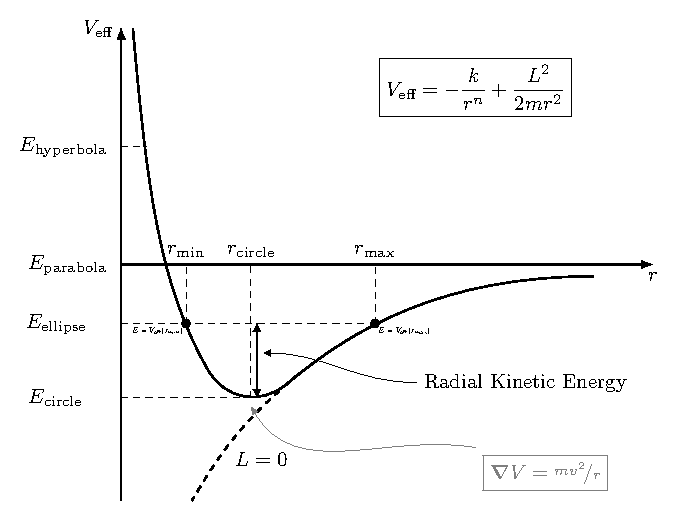
\includegraphics{fig_ch6_effective_potential_well.pdf}
	}
	\caption{Effective potential well $V_{\rm eff}(r) = -k/r^n + L^2/(2mr^2)$, showing the energy levels corresponding to parabolic, circular, elliptical, and hyperbolic orbits, and the turning points $r_{\rm min}, r_{\rm max}$ bounding radial motion at fixed energy $E$.}
	\label{fig:effective_potential_well}
\end{figure}

\textbf{Problem Statement}: The relative-orbit energy derived in Section~\ref{sec:vis_viva}, divided through by $\mu$ (exactly as in Problem 10), reads
\[
\varepsilon\equiv\frac{E}{\mu}=\frac12\dot r^2+v_{\rm eff}(r), \qquad v_{\rm eff}(r)\equiv\frac{\ell^2}{2r^2}-\frac{GM}{r}, \qquad \ell\equiv\frac{L}{\mu},
\]
which is exactly one-dimensional motion in the \emph{effective potential} $v_{\rm eff}(r)$ --- Newtonian gravity's case of the general power-law form $V_{\rm eff}=-k/r^n+L^2/(2mr^2)$ boxed in Figure~\ref{fig:effective_potential_well}, with $n=1$, $k=GM$, $m=1$. Since $\tfrac12\dot r^2\ge0$ always, the radii accessible at fixed $\varepsilon$ are exactly those with $v_{\rm eff}(r)\le\varepsilon$.
\begin{enumerate}[label=(\alph*)]
	\item Find the circular-orbit radius $r_{\rm circle}$ (where $v_{\rm eff}$ is stationary) and the corresponding energy $\varepsilon_{\rm circle}\equiv v_{\rm eff}(r_{\rm circle})$, in terms of $\ell,GM$.
	\item For $\varepsilon_{\rm circle}<\varepsilon<0$, solve $v_{\rm eff}(r)=\varepsilon$ for its two roots $r_{\rm min},r_{\rm max}$, and show they are exactly the periapsis and apoapsis $a(1\mp e)$ already implied by Eqs.~\eqref{eq:visviva_E} and~\eqref{eq:L_of_ae}.
	\item Show that $\varepsilon=\varepsilon_{\rm circle}$, $\varepsilon=0$, and $\varepsilon>0$ correspond respectively to the circular, parabolic, and hyperbolic rows of the eccentricity/conic-section table earlier in this chapter.
	\item An object orbits the Sun ($GM_\odot=1.327\times10^{20}\,\mathrm{m^3\,s^{-2}}$) with $\ell=4.089\times10^{15}\,\mathrm{m^2\,s^{-1}}$ and $\varepsilon=-4.423\times10^{8}\,\mathrm{J\,kg^{-1}}$. Find $r_{\rm min}$, $r_{\rm max}$, and $e$.
\end{enumerate}

\textbf{Detailed Solutions}:
\begin{enumerate}[label=(\alph*)]
	\item Setting $v_{\rm eff}'(r)=-\ell^2/r^3+GM/r^2=0$:
	\[
	\boxed{r_{\rm circle}=\frac{\ell^2}{GM}}, \qquad
	\varepsilon_{\rm circle}=\frac{\ell^2}{2r_{\rm circle}^2}-\frac{GM}{r_{\rm circle}}=\frac{GM}{2r_{\rm circle}}-\frac{GM}{r_{\rm circle}}
	\;\Longrightarrow\;
	\boxed{\varepsilon_{\rm circle}=-\frac{G^2M^2}{2\ell^2}.}
	\]

	\item Multiplying $v_{\rm eff}(r)=\varepsilon$ through by $2r^2$ gives the quadratic $2\varepsilon r^2+2GMr-\ell^2=0$, with roots
	\[
	r=\frac{-GM\pm\sqrt{G^2M^2+2\varepsilon\ell^2}}{2\varepsilon}.
	\]
	Substituting $\varepsilon=-GM/(2a)$ and $\ell^2=GMa(1-e^2)$ (Eqs.~\eqref{eq:visviva_E},~\eqref{eq:L_of_ae} divided by $\mu,\mu^2$) gives $2\varepsilon\ell^2=-G^2M^2(1-e^2)$, so the discriminant collapses to $G^2M^2e^2$, and
	\[
	\boxed{r_{\rm min}=a(1-e), \qquad r_{\rm max}=a(1+e),}
	\]
	the periapsis and apoapsis distances, confirming that the effective-potential turning points and the conic-section geometry are two descriptions of the same orbit.

	\item From $\varepsilon=-GM/(2a)$: $\varepsilon=\varepsilon_{\rm circle}$ forces $r_{\rm min}=r_{\rm max}$, i.e.\ $e=0$ (circular); $\varepsilon=0$ forces $a\to\infty$, i.e.\ $e=1$ (parabolic); $\varepsilon>0$ forces $a<0$, i.e.\ $e>1$ (hyperbolic) --- exactly the classification already tabulated in this chapter.

	\item With $GM=1.327\times10^{20}\,\mathrm{m^3\,s^{-2}}$: $r_{\rm circle}=\ell^2/GM=1.260\times10^{11}\,\mathrm m$, and from $\varepsilon=-GM/(2a)$, $a=-GM/(2\varepsilon)=1.500\times10^{11}\,\mathrm m$. Then $\ell^2=GMa(1-e^2)$ gives $1-e^2=\ell^2/(GMa)=0.8400$, so
	\[
	\boxed{e\simeq0.400, \qquad r_{\rm min}=a(1-e)\simeq9.00\times10^{10}\,\mathrm m, \qquad r_{\rm max}=a(1+e)\simeq2.10\times10^{11}\,\mathrm m.}
	\]
\end{enumerate}

\subsection{Problem 6: Hohmann Transfer Impulses and Energy Budget}

\begin{figure}[htbp]
	\centering
	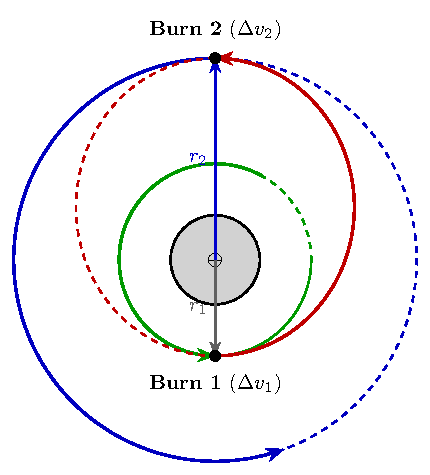
\includegraphics{fig_ch6_hohmann_transfer_ellipse.pdf}
	\caption{Hohmann transfer ellipse between initial low-Earth orbit $r_1$ and geostationary orbit $r_2$.}
	\label{fig:hohmann_transfer_ellipse}
\end{figure}

\textbf{Problem Statement}: A $1000\,\mathrm{kg}$ satellite transfers from an initial circular orbit of period $T_1 = 6\,\mathrm{h}$ to a geostationary orbit ($T_{\rm GEO} \approx 86164\,\mathrm{s}$).
\begin{enumerate}[label=(\alph*)]
	\item Find the intermediate transfer eccentricity $e$.
	\item Find the impulsive velocity boosts $\Delta v_1, \Delta v_2$ and required impulses $P_1, P_2$.
	\item Find the total energy and angular momentum supplied.
\end{enumerate}

\textbf{Solution}:
\begin{enumerate}[label=(\alph*)]
	\item Initial and final radii:
	\[
	r_1 = \left(\frac{\mu_E T_1^2}{4\pi^2}\right)^{1/3} \simeq 1.676 \times 10^7\,\mathrm{m}, \qquad r_2 = \left(\frac{\mu_E T_{\rm GEO}^2}{4\pi^2}\right)^{1/3} \simeq 4.216 \times 10^7\,\mathrm{m}.
	\]
	The transfer ellipse has semi-major axis $a_t = (r_1+r_2)/2$, giving eccentricity:
	\[
	\boxed{e = \frac{r_2-r_1}{r_2+r_1} \simeq 0.431}.
	\]
	\item The circular speeds are $v_{c1} = \sqrt{\mu_E/r_1} \simeq 4.876\,\mathrm{km/s}$ and $v_{c2} = \sqrt{\mu_E/r_2} \simeq 3.075\,\mathrm{km/s}$.
	At perigee of the transfer orbit, $v_p = \sqrt{\mu_E(2/r_1 - 1/a_t)} \simeq 5.833\,\mathrm{km/s}$.
	Thus:
	\[
	\Delta v_1 = v_p - v_{c1} \simeq 0.957\,\mathrm{km/s} \implies \boxed{P_1 = m\Delta v_1 \simeq 9.57 \times 10^5\,\mathrm{N\,s}}.
	\]
	At apogee, $v_a = \sqrt{\mu_E(2/r_2 - 1/a_t)} \simeq 2.319\,\mathrm{km/s}$. Thus:
	\[
	\Delta v_2 = v_{c2} - v_a \simeq 0.755\,\mathrm{km/s} \implies \boxed{P_2 = m\Delta v_2 \simeq 7.55 \times 10^5\,\mathrm{N\,s}}.
	\]
	\item Total energy and angular momentum supplied:
	\[
	\boxed{\Delta E = -\frac{\mu_E m}{2r_2} + \frac{\mu_E m}{2r_1} \simeq 7.16 \times 10^9\,\mathrm{J}},
	\]
	\[
	\boxed{\Delta L = m\sqrt{\mu_E r_2} - m\sqrt{\mu_E r_1} \simeq 4.79 \times 10^{13}\,\mathrm{kg\,m^2\,s^{-1}}}.
	\]
\end{enumerate}

\subsection{Problem 7: Determining Orbital Elements from Initial State Vectors}

\textbf{Problem Statement}: Given initial relative vectors $\vec r_0, \vec v_0$ at $t=0$, derive the orbital elements $(a, e, \Omega, i, \omega, T_0)$.

\textbf{Solution}:
\begin{enumerate}[label=(\alph*)]
	\item Conserved specific energy $\epsilon = v_0^2/2 - k/r_0$, specific angular momentum $\vec h = \vec r_0 \times \vec v_0$, Runge--Lenz vector $\vec A = \vec v_0 \times \vec L - k\mu\hat r_0$.
	\item Orbital elements:
	\[
	a = \left(\frac{2}{r_0} - \frac{v_0^2}{k}\right)^{-1}, \qquad e = \frac{|\vec A|}{k\mu}, \qquad n = \sqrt{\frac{k}{a^3}}, \qquad i = \arccos\left(\frac{h_z}{h}\right).
	\]
	With ascending node vector $\vec N = \hat z \times \vec h$:
	\[
	\Omega = \operatorname{atan2}(N_y, N_x), \qquad \omega = \operatorname{atan2}\left(\frac{\hat h \cdot (\vec N \times \vec e)}{Ne}, \frac{\vec N \cdot \vec e}{Ne}\right).
	\]
	The initial true anomaly $v_0$ and eccentric anomaly $u_0$ yield the time of periapsis passage:
	\[
	T_0 = -\frac{u_0 - e\sin u_0}{n}.
	\]
\end{enumerate}

\subsection{Problem 8: Continuous Tangential Thrust Orbital Evolution}

\textbf{Problem Statement}: A $500\,\mathrm{kg}$ satellite initially moves in a circular Earth orbit of period $T = 8\,\mathrm{h}$. At $t=0$, a $100\,\mathrm{N}$ thruster is switched on such that the thrust is always directed parallel to the instantaneous velocity vector ($\vec A = A\hat v$).
\begin{enumerate}[label=(\alph*)]
	\item Find the initial orbital radius $a(0)$.
	\item Derive the rate of change of the semi-major axis $\dot a$.
	\item Derive the rate of change of the eccentricity $\dot e$ from the exact rate of the Laplace--Runge--Lenz vector $\vec A$.
	\item Can the coupled evolution equations for $(a, e)$ be solved analytically?
\end{enumerate}

\textbf{Essential Ideas}:
\begin{itemize}
	\item \textbf{Thrust Acceleration and Initial Radius}: The continuous thrust acceleration is $A = F/m = 100\,\mathrm{N}/500\,\mathrm{kg} = 0.2\,\mathrm{m\cdot s^{-2}}$. For an initially circular orbit ($e=0$) of period $T = 8\,\mathrm{h} = 28{,}800\,\mathrm{s}$ around Earth ($\mu_E \equiv GM_\oplus \approx 3.986 \times 10^{14}\,\mathrm{m^3\cdot s^{-2}}$), Kepler's third law gives:
	\[
	a(0) = \left(\frac{\mu_E T^2}{4\pi^2}\right)^{1/3} \simeq 2.03 \times 10^7\,\mathrm{m} \approx 20{,}300\,\mathrm{km}.
	\]
	\item \textbf{Perturbation Force Vector}: Because thrust is tangential, $\vec a_{\rm thrust} = A\hat v$. In polar coordinates $(\hat r, \hat\phi)$, velocity is $\vec v = \dot r\hat r + r\dot\phi\hat\phi = \dot r\hat r + \frac{L}{\mu r}\hat\phi$. The perturbing force $\vec F = \mu A\hat v = F_r\hat r + F_\phi\hat\phi$ has components:
	\[
	F_r = \mu A\frac{\dot r}{v}, \qquad F_\phi = \mu A\frac{L}{\mu r v} = \frac{AL}{rv}.
	\]
	Using $\xi \equiv \frac{\mu r\dot r}{L} = \frac{e\sin f}{1+e\cos f}$ (Eq.~\eqref{eq:xi_def}), the radial force satisfies $F_r = \xi F_\phi = \frac{\xi L}{r}\frac{A}{v}$.
\end{itemize}

\textbf{Detailed Solutions}:
\begin{enumerate}[label=(\alph*)]
	\item \textbf{Initial Semi-Major Axis}:
	\[
	\boxed{a(0) = \left(\frac{\mu_E T^2}{4\pi^2}\right)^{1/3} = \left(\frac{3.986 \times 10^{14} \times (28800)^2}{4\pi^2}\right)^{1/3} \simeq 2.03 \times 10^7\,\mathrm{m}}.
	\]

	\item \textbf{Evolution of Semi-Major Axis $\dot a$}:
	The work done per unit time by the tangential thrust on the orbiting mass is:
	\[
	\dot E = \vec F \cdot \vec v = (\mu A\hat v)\cdot\vec v = \mu A v.
	\]
	The specific orbital energy $\epsilon = E/\mu = -\mu_E / (2a)$ changes at the rate $\dot\epsilon = Av$. Differentiating:
	\[
	\dot\epsilon = \frac{\mu_E}{2a^2}\dot a \implies \dot a = \frac{2a^2}{\mu_E}Av.
	\]
	From the vis-viva equation $v^2 = \mu_E\left(\frac{2}{r} - \frac{1}{a}\right) = \frac{\mu_E}{a}\left(\frac{1+2e\cos f + e^2}{1-e^2}\right)$, the exact rate of change of the semi-major axis is:
	\begin{equation}
		\boxed{\frac{da}{dt} = 2A\sqrt{\frac{a^3}{\mu_E}}\sqrt{\frac{1+2e\cos f+e^2}{1-e^2}}}.
		\label{eq:prob8_adot}
	\end{equation}

	\item \textbf{Evolution of Eccentricity $\dot e$ via the Laplace--Runge--Lenz Vector}:
	The Laplace--Runge--Lenz vector $\vec A = \vec p\times\vec L - GM\mu^2\hat r$ has magnitude $A = GM\mu^2 e = \mu_E\mu^2 e$ and points along the periapsis direction $\hat A = \cos f\hat r - \sin f\hat\phi$ (Eq.~\eqref{eq:Ahat_f}).
	
	Under a general planar perturbing force $\vec F = F_r\hat r + F_\phi\hat\phi$, the exact rate of change of $\vec A$ from Eq.~\eqref{eq:planar_Adot_xi} is:
	\[
	\dot{\vec A} = \vec F\times\vec L + \vec p\times(\vec r\times\vec F) = L\left[2F_\phi\hat r - (F_r + \xi F_\phi)\hat\phi\right].
	\]
	Since $\hat A \cdot \hat A = 1 \implies \hat A \cdot \dot{\hat A} = 0$, the scalar rate $\dot A$ is obtained by projecting $\dot{\vec A}$ along $\hat A$:
	\begin{align*}
		\dot A &= \dot{\vec A}\cdot\hat A = L\left[2F_\phi\hat r - (F_r+\xi F_\phi)\hat\phi\right]\cdot (\cos f\hat r - \sin f\hat\phi) \\
		&= L\left[ 2F_\phi\cos f + (F_r + \xi F_\phi)\sin f \right] \\
		&= L\left[ F_r\sin f + F_\phi(2\cos f + \xi\sin f) \right].
	\end{align*}
	Evaluating this on the instantaneous osculating orbit with $A = \mu_E\mu^2 e$ and $L = \mu\sqrt{\mu_E a(1-e^2)}$ yields Gauss's variational equation for eccentricity (Eq.~\eqref{eq:gauss_edot}):
	\begin{equation}
		\dot e = \sqrt{\frac{a(1-e^2)}{\mu_E\mu^2}}\left[ F_r\sin f + F_\phi(2\cos f + \xi\sin f) \right].
	\end{equation}
	Now substituting the specific components for tangential thrust, $F_r = \xi F_\phi = \frac{\xi L}{r}\frac{A}{v}$ and $F_\phi = \frac{L}{r}\frac{A}{v}$:
	\begin{align*}
		F_r\sin f + F_\phi(2\cos f + \xi\sin f) &= \frac{AL}{rv}\left[ \xi\sin f + 2\cos f + \xi\sin f \right] \\
		&= \frac{2AL}{rv}\left(\cos f + \xi\sin f\right).
	\end{align*}
	Using $\xi = \frac{e\sin f}{1+e\cos f}$:
	\[
	\cos f + \xi\sin f = \cos f + \frac{e\sin^2 f}{1+e\cos f} = \frac{\cos f(1+e\cos f) + e\sin^2 f}{1+e\cos f} = \frac{\cos f + e}{1+e\cos f}.
	\]
	Combining this with $\frac{L}{r} = \frac{\mu\sqrt{\mu_E a(1-e^2)}}{a(1-e^2)/(1+e\cos f)} = \frac{\mu\sqrt{\mu_E}(1+e\cos f)}{\sqrt{a(1-e^2)}}$:
	\begin{align*}
		\dot e &= \sqrt{\frac{a(1-e^2)}{\mu_E\mu^2}} \cdot \frac{2A}{v} \left[\frac{\mu\sqrt{\mu_E}(1+e\cos f)}{\sqrt{a(1-e^2)}}\right] \left[\frac{\cos f + e}{1+e\cos f}\right] \\
		&= \frac{2A}{v}(\cos f + e).
	\end{align*}
	Expressing $v$ in terms of orbital elements via the vis-viva equation:
	\begin{equation}
		\boxed{\frac{de}{dt} = 2A\left(\frac{\cos f + e}{v}\right) = 2A\sqrt{\frac{a(1-e^2)}{\mu_E}}\left(\frac{\cos f + e}{\sqrt{1+2e\cos f+e^2}}\right)}.
		\label{eq:prob8_edot}
	\end{equation}
	\textbf{Remark}: Unlike naive differentiation of $e^2 = 1 + 2\epsilon h^2/\mu_E^2$ (which yields an ill-defined $0/0$ singularity dividing by $e$ at $e=0$), the Runge--Lenz vector rate directly gives the well-behaved, non-singular initial rate $\dot e\big|_{e=0} = 2A\sqrt{a/\mu_E}\cos f$.

	\item \textbf{Analytical Solvability}:
	Equations~\eqref{eq:prob8_adot} and~\eqref{eq:prob8_edot} do not form a closed autonomous two-dimensional dynamical system because both derivatives depend explicitly on the instantaneous orbital phase $f(t)$ (true anomaly). The phase itself evolves according to:
	\[
	\dot f = \frac{L}{\mu r^2} + \dot\omega,
	\]
	where the periapsis precession rate $\dot\omega$ is also driven by the perturbing force. Because the continuous thrust continuously alters the orbit throughout each revolution, the coupled system $(a(t), e(t), f(t))$ cannot be solved in closed elementary analytical form. In mission design and orbital mechanics, it is solved by numerical integration or by \emph{orbit averaging} ($\langle\dot a\rangle = \frac{1}{2\pi}\int_0^{2\pi}\dot a\,df$) over each complete orbital period.
\end{enumerate}

\subsection{Problem 9: Double-Lined Spectroscopic Binary --- Radial Velocities and Masses}
\label{prob:sb2}

\textbf{Problem Statement}: In a \emph{double-lined spectroscopic binary} (SB2), we see absorption lines from \emph{both} stars in the combined spectrum. Each line is Doppler-shifted by that star's own orbital motion around the center of mass. A Doppler shift only measures the \emph{radial velocity} $v_r\equiv\vec v\cdot\hat R$, the part of a star's velocity along the line of sight $\hat R$. Motion across the sky (perpendicular to $\hat R$) does not stretch or compress the wavelength, so it leaves no Doppler signal at all. That sideways motion only shows up as proper motion (Chapter~3), not in the spectrum. Tracking each star's wavelength shift separately gives two radial-velocity curves, $v_{r,1}(t)$ and $v_{r,2}(t)$. Both share the same period $P$ and eccentricity $e$, but usually have different semi-amplitudes $K_1$ and $K_2$ (Figures~\ref{fig:sb2_schematic} and \ref{fig:sb2_rvcurve}). A particular system is measured to have $P=4.20\,\mathrm{d}$, $e=0.15$, $K_1=88\,\mathrm{km\,s^{-1}}$, and $K_2=132\,\mathrm{km\,s^{-1}}$.
\begin{enumerate}[label=(\alph*)]
	\item Without knowing the orbital inclination $i$, what can already be said about the mass ratio $m_1/m_2$?
	\item Derive $(m_1+m_2)\sin^3i$ in terms of $P$, $K_1$, $K_2$, and $e$, and evaluate it numerically.
	\item Hence find $m_1\sin^3i$ and $m_2\sin^3i$ individually.
	\item This same system is also observed to be eclipsing, so $i\simeq90^\circ$. What are the actual masses $m_1$ and $m_2$?
\end{enumerate}

\begin{figure}[htbp]
	\centering
	\begin{minipage}[t]{0.48\textwidth}
		\centering
		\resizebox{\linewidth}{!}{%
		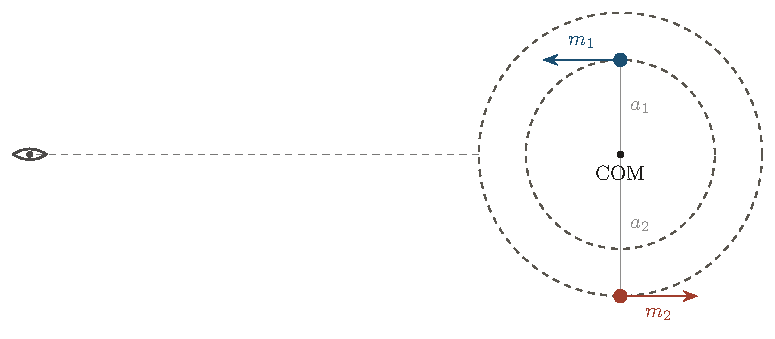
\includegraphics{fig_ch6_sb2_schematic.pdf}%
		}
		\caption{A binary at quadrature, with $m_1$, $m_2$, and the COM in a line. $m_1$ moves away and $m_2$ moves toward the observer, along the line of sight $\hat R$.}
		\label{fig:sb2_schematic}
	\end{minipage}
	\hfill
	\begin{minipage}[t]{0.48\textwidth}
		\centering
		\resizebox{\linewidth}{!}{%
		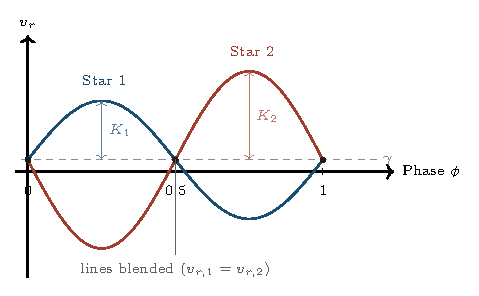
\includegraphics{fig_ch6_sb2_rvcurve.pdf}%
		}
		\caption{Radial-velocity curves for both stars, circular-orbit case. Anti-phase sine curves about $\gamma$, with semi-amplitudes $K_1\neq K_2$.}
		\label{fig:sb2_rvcurve}
	\end{minipage}
\end{figure}

\textbf{Essential Ideas}:
\begin{itemize}
	\item Start from $\vec r_1=(m_2/M)\vec r$, $\vec r_2=-(m_1/M)\vec r$ (Problem 1). Differentiate and project onto $\hat R$.
	\[
	v_{r,1}-\gamma = \frac{m_2}{M}\,v_{r,\rm rel}, \qquad v_{r,2}-\gamma = -\frac{m_1}{M}\,v_{r,\rm rel}, \qquad \gamma\equiv\vec V_{\rm CM}\cdot\hat R,
	\]
	Here $v_{r,\rm rel}\equiv v_{r,1}-v_{r,2}$, and $\gamma$ is constant (Eq.~\eqref{eq:comEOM}). This holds at every phase. So
	\[
	\frac{K_1}{K_2}=\frac{m_2}{m_1},
	\]
	no matter what $i$ and $e$ are.
	\item A Keplerian orbit's line-of-sight speed has semi-amplitude $K=2\pi a\sin i/(P\sqrt{1-e^2})$. Apply this to the relative orbit ($a=a_1+a_2$). Then $v_{r,\rm rel}=v_{r,1}-v_{r,2}$ has amplitude $K_1+K_2$.
\end{itemize}

\textbf{Detailed Solutions}:
\begin{enumerate}[label=(\alph*)]
	\item \textbf{Mass ratio}.
	\[
	\boxed{\frac{m_1}{m_2}=\frac{K_2}{K_1}=\frac{132}{88}=1.50.}
	\]

	\item \textbf{Total mass}. Apply $K=2\pi a\sin i/(P\sqrt{1-e^2})$ to the relative orbit (amplitude $K_1+K_2$), and use Kepler's third law, $P^2=4\pi^2a^3/[G(m_1+m_2)]$.
	\[
	(m_1+m_2)\sin^3i=\frac{4\pi^2(a\sin i)^3}{GP^2} = \frac{P(K_1+K_2)^3(1-e^2)^{3/2}}{2\pi G}.
	\]
	Use $P=3.629\times10^5\,\mathrm s$, $K_1+K_2=2.20\times10^5\,\mathrm{m\,s^{-1}}$, $(1-e^2)^{3/2}=0.966$.
	\[
	\boxed{(m_1+m_2)\sin^3i \simeq 8.91\times10^{30}\,\mathrm{kg}\simeq 4.48\,M_\odot.}
	\]

	\item \textbf{Individual masses}. Use $m_1=\dfrac{K_2}{K_1+K_2}(m_1+m_2)$, $m_2=\dfrac{K_1}{K_1+K_2}(m_1+m_2)$, the same COM weighting as (a).
	\[
	\boxed{m_1\sin^3i \simeq 2.69\,M_\odot,\qquad m_2\sin^3i \simeq 1.79\,M_\odot.}
	\]

	\item \textbf{Eclipsing case}. $i\simeq90^\circ$, so $\sin^3i\simeq1$ and the factors in (c) drop out directly.
	\[
	\boxed{m_1\simeq2.69\,M_\odot, \qquad m_2\simeq1.79\,M_\odot.}
	\]
	Double-lined eclipsing binaries are valuable for exactly this reason. Both masses, and from the light curve both radii, come out this way, with almost no model assumptions.
\end{enumerate}

\subsection{Problem 10: Dynamical Mass of a Host Halo from a Satellite's Orbit}
\label{prob:halo_mass}

\textbf{Problem Statement}: A satellite of mass $m_s$ (for example a dwarf galaxy or globular cluster) orbits a much bigger dark-matter halo of mass $M_h$. We measure its present distance $r$ from the Galactic center and its full space velocity $\vec v$ (from proper motion plus radial velocity). We also estimate its orbital eccentricity $e$ independently, for example from similar orbits in cosmological simulations. As in Section~\ref{sec:com_separation}, let $M\equiv m_s+M_h$ be the total mass and $\mu\equiv m_sM_h/M$ the reduced mass. If the satellite sits well outside the halo's inner mass, we can treat the halo as a point mass. Then the satellite follows an ordinary Keplerian orbit, with energy $E=-GM\mu/(2a)$ (Eq.~\eqref{eq:visviva_E}) and angular momentum $\vec L=\mu\,\vec r\times\vec v$, $L^2=GM\mu^2a(1-e^2)$ (Eq.~\eqref{eq:L_of_ae}).
\begin{enumerate}[label=(\alph*)]
	\item Show that $\mu$ cancels out of both the vis-viva equation and the angular-momentum relation, leaving two equations in the directly observable quantities $r$, $v$, and $\ell\equiv|\vec r\times\vec v|=L/\mu$. Combine them to show that the total mass $M$ satisfies
	\[
	\frac{G^2(1-e^2)}{\ell^2}M^2-\frac{2G}{r}M+v^2=0,
	\]
	and solve for $M$ in terms of $r,v,\ell,e$.
	\item Suppose instead the satellite happens to be caught exactly at apocenter, where the velocity is purely tangential ($\vec v\perp\vec r$) and $r=r_{\rm apo}=a(1+e)$. Show that the mass estimate then collapses to the much simpler
	\[
	M=\frac{v_{\rm apo}^2\,r_{\rm apo}}{G(1-e)}.
	\]
	\item A dwarf satellite is observed at apocenter with $r_{\rm apo}=250\,\mathrm{kpc}$ and $v_{\rm apo}=95\,\mathrm{km\,s^{-1}}$, and its orbit is modeled to have $e=0.6$. Evaluate $M$, in kg and in $M_\odot$, and argue that it is an excellent estimate of $M_h$ alone.
	\item Eccentricity is only one possible choice of the ``extra'' datum used here. What property of the governing equations makes some third quantity beyond $(r,v)$ necessary at all, and what else could play that role?
	\item This method returns only the total mass $M=m_s+M_h$, never $m_s$ and $M_h$ separately. Explain why no amount of additional \emph{orbital} data --- more precise $r$, $v$, or $e$, or even more satellites on more orbits --- could ever split $M$ into $m_s$ and $M_h$ individually, and say what kind of information could.
\end{enumerate}

\textbf{Essential Ideas}:
\begin{itemize}
	\item $\mu$ cancels. Just as in the vis-viva equation ($v^2=GM(2/r-1/a)$, Sec.~\ref{sec:vis_viva}), the orbit's shape and motion depend on $m_s,M_h$ only through $M$. $\mu$ drops out once $E,L$ are turned into relations among $r,v,\ell\equiv|\vec r\times\vec v|$.
	\item There are three unknowns $(a,e,M)$ but only two equations relating $(r,v,\ell)$. So one more independent piece of data is needed, and $e$ is the usual choice.
	\item At apocenter $\dot r=0$, so $v$ is purely tangential and $r_{\rm apo}=a(1+e)$ directly, without needing $\ell$.
	\item Test-particle limit. Since $m_s\ll M_h$, $M=m_s+M_h$ is almost exactly $M_h$.
	\item \textbf{Degeneracy, not just ignorance}. $\mu$ is the one combination of $m_s,M_h$ that is \emph{not} their sum, and it cancels completely from both relations. So every orbital observable depends on the masses only through $M$, and any split of $M$ gives the identical orbit. This is different from Problem~9's mass \emph{ratio}, where two tracers gave one comparison. Here there is only one tracer, so only one orbit.
\end{itemize}

\textbf{Detailed Solutions}:
\begin{enumerate}[label=(\alph*)]
	\item \textbf{General mass estimator}. Divide $E=\frac12\mu v^2-\dfrac{GM\mu}{r}=-\dfrac{GM\mu}{2a}$ by $\mu$ to recover vis-viva. Divide $L^2=GM\mu^2a(1-e^2)$ by $\mu^2$ and write $\ell\equiv L/\mu=|\vec r\times\vec v|$, which needs no mass.
	\[
	v^2=GM\left(\frac2r-\frac1a\right),\qquad \ell^2=GMa(1-e^2)\;\Longrightarrow\;a=\frac{\ell^2}{GM(1-e^2)}.
	\]
	Substituting,
	\[
	v^2=\frac{2GM}{r}-\frac{G^2M^2(1-e^2)}{\ell^2}
	\;\Longrightarrow\;
	\boxed{\frac{G^2(1-e^2)}{\ell^2}M^2-\frac{2G}{r}M+v^2=0,}
	\]
	a quadratic in $M$, giving
	\[
	\boxed{M=\frac{\ell^2}{G(1-e^2)}\left[\frac1r\pm\sqrt{\frac{1}{r^2}-\frac{(1-e^2)v^2}{\ell^2}}\right],}
	\]
	with $M>0$ selecting the physical root.

	\item \textbf{Apocenter simplification}. Here $\dot r=0$, and $r=r_{\rm apo}=a(1+e)$, so $1/a=(1+e)/r_{\rm apo}$.
	\[
	v_{\rm apo}^2=GM\left(\frac{2}{r_{\rm apo}}-\frac{1+e}{r_{\rm apo}}\right)=\frac{GM(1-e)}{r_{\rm apo}}
	\;\Longrightarrow\;
	\boxed{M=\frac{v_{\rm apo}^2\,r_{\rm apo}}{G(1-e)}.}
	\]
	(Matches part (a) at apocenter, where $\ell=r_{\rm apo}v_{\rm apo}$.)

	\item \textbf{Numerical evaluation}. Use $r_{\rm apo}=7.714\times10^{21}\,\mathrm m$, $v_{\rm apo}=9.5\times10^4\,\mathrm{m\,s^{-1}}$, $e=0.6$.
	\[
	M=\frac{(9.5\times10^4)^2(7.714\times10^{21})}{(6.674\times10^{-11})(1-0.6)}
	\;\Longrightarrow\;
	\boxed{M\simeq2.61\times10^{42}\,\mathrm{kg}\simeq1.31\times10^{12}\,M_\odot,}
	\]
	which is typical for a Milky-Way-sized halo. Dwarf-satellite masses ($10^4$--$10^8\,M_\odot$) are tiny next to this, so $M\simeq M_h$ to six figures.

	\item \textbf{Why a third datum is unavoidable}. $(r,v)$ give two independent numbers, but the orbit has three unknowns $(a,e,M)$, related by only two equations (vis-viva, and $\ell^2=GMa(1-e^2)$). So we need one more independent piece of data to close the system. It could be $e$, as used here, or $\ell$ itself, or the time elapsed since a known pericenter passage, found from Kepler's equation (Sec.~\ref{sec:kepler_equation}). This last option is the basis of the Local Group timing argument for the Milky Way--M31 mass.

	\item \textbf{The barycenter location is the missing parameter}. To specify $\vec x_s(t)$ and $\vec x_h(t)$ separately, we need the six orbital elements $(a,e,i,\Omega,\omega,t_p)$ of the \emph{relative} orbit $\vec r\equiv\vec x_s-\vec x_h$, the total mass $M$, and one more number. Those six elements describe only the shape, orientation, and timing of $\vec r(t)$. They say nothing about where the pair sits in space or how the total mass $M$ is split between the two bodies, and it is that split we are still missing. The extra number is the mass fraction $f\equiv M_h/M$, which is the same as the barycenter's location on the line joining the two bodies. Parts (a)--(d) only give us the first seven, $(a,e,M)$. The relative orbit cannot see $f$, and this is an exact symmetry, not just a practical limit. Newton's third law gives $\ddot{\vec x}_s=-GM_h\hat r/r^2$ and $\ddot{\vec x}_h=Gm_s\hat r/r^2$, so
	\[
	\ddot{\vec r}=\ddot{\vec x}_s-\ddot{\vec x}_h=-\frac{GM}{r^2}\hat r,
	\]
	which depends on $m_s$ and $M_h$ only through $M$. So $\vec r(t)$ stays exactly the same under $m_s\to m_s+\delta$, $M_h\to M_h-\delta$ at fixed $M$. No relative-orbit measurement, however precise, can pin down $f$.

	The individual position $\vec x_s=\vec x_{\rm cm}+(M_h/M)\vec r$ does depend on $f$. And $f=r_s/r$ is a purely geometric ratio, so it needs no dynamics to measure. This is exactly the missing eighth parameter. It is the same idea as Problem~1, where $m_1/m_2=a_2/a_1$ came from each star's distance to the visible barycenter.

	For a satellite and its halo, the problem is one of scale, not principle. Since $m_s/M_h\sim10^{-6}$--$10^{-8}$, the barycenter sits only a tiny fraction of $r_s$ from the halo's center, far too small to measure astrometrically (unlike Problem~1's pair of comparable masses). Without $f$, we instead estimate $m_s$ some other way, for example from its luminosity via a mass-to-light ratio, or from its own internal velocity dispersion via the virial theorem ($M \sim \sigma_v^2 R / G$). Then $M_h=M-m_s$.
\end{enumerate}

\subsection{Problem 11: The Line-of-Sight Direction, in Matrices and Without Them}

\textbf{Problem Statement}: Both Problem 9 (the radial-velocity amplitude $K$) and Problem 10 (the mass estimator built on $\vec V_{\rm CM}\cdot\hat R$) projected an orbital quantity onto the line of sight $\hat R$ without ever pinning down what $\hat R$ \emph{is} in terms of the orbital elements $(i,\Omega,\omega)$.
\begin{enumerate}[label=(\alph*)]
	\item Starting from the rotation relating the orbital frame $(\hatn,\hat y,\hat L)$ to the observer frame $(\hat\alpha,\hat\delta,\hat R)$, Eq.~\eqref{eq:orbital_frame_rotation}, invert it to express $\hat R$ in terms of $\hatn,\hat y,\hat L$. Show that the result does not depend on $\Omega$ at all.
	\[
	\hat R = \sin\iota\,\hat y+\cos\iota\,\hat L.
	\]
	\item Rederive the same identity without any matrix algebra. Use only two facts. First, the node line $\hatn$ is, by construction, the intersection of the orbital plane and the sky plane. Second, the inclination is the angle between the two planes' normals, $\hat L$ and $\hat R$.
	\item A body follows a Keplerian orbit of elements $(a,e,i,\omega)$ in the plane spanned by $\hatn,\hat y$, at true anomaly $f$ (so its polar angle from $\hatn$ is $\phi=\omega+f$). Using $\hat R=\sin\iota\,\hat y+\cos\iota\,\hat L$ together with the fact that $\vec v$ lies entirely in the orbital plane, show that the line-of-sight (radial) velocity $v_r=\vec v\cdot\hat R$ takes the form
	\[
	v_r = \gamma + K\big[\cos(\omega+f)+e\cos\omega\big],
	\]
	and identify $K$ in terms of $G$, $M$, $a$, $e$, $i$.
	\item Using Kepler's third law, show that this $K$ is exactly the semi-amplitude $K=2\pi a\sin i/(P\sqrt{1-e^2})$ quoted without proof in Problem 9.
\end{enumerate}

\textbf{Essential Ideas}:
\begin{itemize}
	\item A rotation matrix is orthogonal, so $R^{-1}=R^T$. Undoing it costs no more than transposing and reversing the product order.
	\item Simple geometric facts about an orthonormal triad, such as which vectors are perpendicular, or what a named angle is the cosine of, can rebuild a rotation result with less algebra than the matrix itself.
	\item Angular momentum conservation confines $\vec r,\vec v$ to the orbital plane, so $\vec r\cdot\hat L=\vec v\cdot\hat L=0$. This drops $\hat L$ from $v_r=\vec v\cdot\hat R$ in part (c).
\end{itemize}

\textbf{Detailed Solutions}:
\begin{enumerate}[label=(\alph*)]
	\item \textbf{Matrix version}. Both $3\times3$ factors in Eq.~\eqref{eq:orbital_frame_rotation} are rotation matrices, so they are orthogonal, $R^{-1}=R^T$. Inverting the product just reverses the order and transposes each factor.
	\begin{align*}
	\begin{pmatrix}\hat\alpha\\\hat\delta\\\hat R\end{pmatrix}
	&=\begin{pmatrix}\cos\Omega&\sin\Omega&0\\-\sin\Omega&\cos\Omega&0\\0&0&1\end{pmatrix}^{\!T}
	\begin{pmatrix}1&0&0\\0&\cos\iota&\sin\iota\\0&-\sin\iota&\cos\iota\end{pmatrix}^{\!T}
	\begin{pmatrix}\hatn\\\hat y\\\hat L\end{pmatrix}\\[4pt]
	&=\begin{pmatrix}\cos\Omega&-\sin\Omega&0\\\sin\Omega&\cos\Omega&0\\0&0&1\end{pmatrix}
	\begin{pmatrix}1&0&0\\0&\cos\iota&-\sin\iota\\0&\sin\iota&\cos\iota\end{pmatrix}
	\begin{pmatrix}\hatn\\\hat y\\\hat L\end{pmatrix}.
	\end{align*}
	Multiply the two matrices, and read off the third row, the coefficients of $\hat R$.
	\[
	\hat R = \underbrace{(0)}_{\hatn\text{-coefficient}}\hatn+\sin\iota\,\hat y+\cos\iota\,\hat L
	\;\Longrightarrow\;
	\boxed{\hat R=\sin\iota\,\hat y+\cos\iota\,\hat L,}
	\]
	since $\Omega$ only enters the $\hatn$-mixing block, which never touches the row producing $\hat R$.

	\item \textbf{Geometric version}. $\hatn$ is the intersection of the orbital and sky planes. So it is perpendicular to both planes' normals, $\hatn\cdot\hat L=0$ and $\hatn\cdot\hat R=0$. Since $\{\hatn,\hat y,\hat L\}$ is orthonormal, any unit vector with zero $\hatn$-component is a combination of $\hat y,\hat L$ alone.
	\[
	\hat R = (\hat R\cdot\hat y)\,\hat y+(\hat R\cdot\hat L)\,\hat L.
	\]
	By definition, $i$ is the angle between the planes' normals, so $\hat R\cdot\hat L=\cos\iota$. Since $\hat R\cdot\hatn=0$ and $\hat R$ is a unit vector, $(\hat R\cdot\hat y)^2=\sin^2\iota$. The orientation convention, that $\hat y$ leads $\hatn$ by $90^\circ$ toward $\hat R$, fixes the sign.
	\[
	\boxed{\hat R=\sin\iota\,\hat y+\cos\iota\,\hat L,}
	\]
	the same as part (a), with no matrix multiplied.

	\item \textbf{Radial velocity}. Angular momentum conservation confines the orbit to the plane spanned by $\hatn,\hat y$, so $\vec v\cdot\hat L=0$, and
	\[
	v_r=\vec v\cdot\hat R = \sin\iota\,(\vec v\cdot\hat y).
	\]
	With $\vec r=r\cos\phi\,\hatn+r\sin\phi\,\hat y$ and the planar-polar velocity $\vec v=\dot r\,\hat r+r\dot\phi\,\hat\phi$,
	\[
	\vec v\cdot\hat y = \dot r\sin\phi+r\dot\phi\cos\phi.
	\]
	Substitute $\dot r=\dfrac{Le\sin f}{\mu\lambda}$ (Eq.~\eqref{eq:rdot_true_anomaly}) and $r\dot\phi=\dfrac{L}{\mu r}=\dfrac{L(1+e\cos f)}{\mu\lambda}$ (Eq.~\eqref{eq:theta_dot_keplerian}), with $\phi=\omega+f$.
	\[
	\vec v\cdot\hat y = \frac{L}{\mu\lambda}\Big[e\sin f\sin(\omega+f)+(1+e\cos f)\cos(\omega+f)\Big]
	=\frac{L}{\mu\lambda}\Big[\cos(\omega+f)+e\cos\omega\Big],
	\]
	using $\sin f\sin(\omega+f)+\cos f\cos(\omega+f)=\cos\omega$. Since $L=\mu\sqrt{GM\lambda}$ (Eq.~\eqref{eq:L_of_ae}) and $\lambda=a(1-e^2)$, we get $L/(\mu\lambda)=\sqrt{GM/[a(1-e^2)]}$. Add back $\gamma$, Problem 9's line-of-sight COM velocity, as the baseline.
	\[
	v_r = \sin\iota\sqrt{\frac{GM}{a(1-e^2)}}\Big[\cos(\omega+f)+e\cos\omega\Big] + \gamma.
	\]
	Matching to the stated form,
	\[
	\boxed{K=\sin\iota\sqrt{\frac{GM}{a(1-e^2)}}.}
	\]

	\item \textbf{Consistency with Problem 9}. Kepler's third law gives $GM=4\pi^2a^3/P^2$, so
	\[
	K=\sin\iota\sqrt{\frac{4\pi^2a^3/P^2}{a(1-e^2)}}=\sin\iota\sqrt{\frac{4\pi^2a^2}{P^2(1-e^2)}}
	\;\Longrightarrow\;
	\boxed{K=\frac{2\pi a\sin\iota}{P\sqrt{1-e^2}},}
	\]
	the radial-velocity semi-amplitude of a spectroscopic binary, Problem 9's $K$.
\end{enumerate}

\subsection{Problem 12: The Gravitational Slingshot}

\textbf{Problem Statement}: A spacecraft flies by Jupiter. Jupiter's own speed around the Sun is $V_p\simeq13.1\,\mathrm{km\,s^{-1}}$. Relative to Jupiter, the spacecraft moves on a hyperbolic orbit with $e=1.2$ and $v_\infty=10\,\mathrm{km\,s^{-1}}$ (Eq.~\eqref{eq:vinf}). Find the change in the spacecraft's speed around the Sun, given that its speed relative to Jupiter cannot change.

\begin{figure}[htbp]
	\centering
	\resizebox{0.68\textwidth}{!}{%
	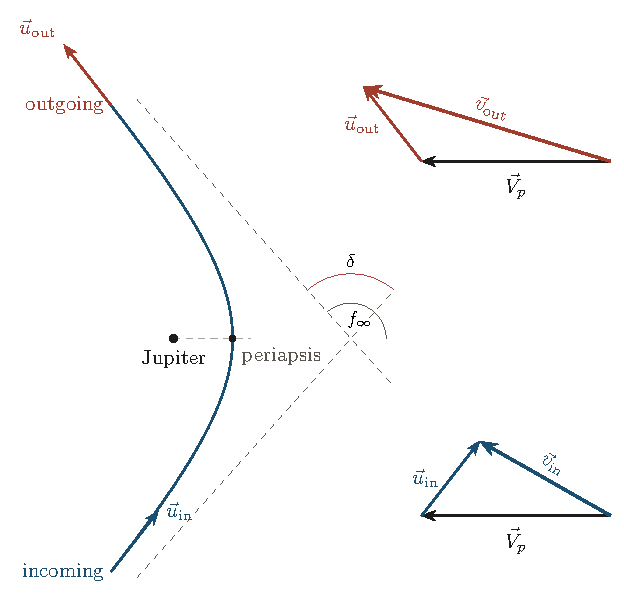
\includegraphics{fig_ch6_slingshot_classic.pdf}%
	}
	\caption{The gravitational slingshot. Left, Jupiter's frame. The dashed lines are the true asymptotes, crossing at the hyperbola's center, with $\delta$ between them and $f_\infty$ from periapsis. $\vec u_{\rm in}$ and $\vec u_{\rm out}$ are the true tangent directions. Right, $\vec u_{\rm in}$ and $\vec u_{\rm out}$ moved (parallel-transported) onto Jupiter's heliocentric velocity $\vec V_p$.}
	\label{fig:slingshot_classic}
\end{figure}

\textbf{Solution}. In the solar frame, we drop the Jupiter--Sun terms that do not involve $\vec x_{\rm sc}$.
\begin{equation}
	L = \frac12 m_{\rm sc}\dot{\vec x}_{\rm sc}^2 + \frac{GM_\odot m_{\rm sc}}{|\vec x_{\rm sc}|} + \frac{Gm_{\rm sc}M_J}{|\vec x_{\rm sc}-\vec X_J(t)|}.
\end{equation}
Let $\vec r\equiv\vec x_{\rm sc}-\vec X_J(t)$. Over the brief encounter, $\vec X_J(t)\approx\vec X_{J,0}+\vec V_pt$ and $|\vec x_{\rm sc}|\approx X_J(t)$, dropping the small term $O(r/X_J)$. Also $\dot{\vec x}_{\rm sc}=\vec V_p+\dot{\vec r}$, so
\begin{align}
	L &\approx \underbrace{\tfrac12m_{\rm sc}V_p^2+\dfrac{GM_\odot m_{\rm sc}}{X_J(t)}}_{f(t)} + \underbrace{m_{\rm sc}\vec V_p\cdot\dot{\vec r}}_{\frac{d}{dt}(m_{\rm sc}\vec V_p\cdot\vec r)} + \frac12m_{\rm sc}\dot{\vec r}^2+\frac{Gm_{\rm sc}M_J}{r}\\
	&\Longrightarrow\quad L(\vec r,\dot{\vec r}) = \frac12m_{\rm sc}\dot{\vec r}^2+\frac{Gm_{\rm sc}M_J}{r},
	\label{eq:slingshot_effective_L}
\end{align}
this has no explicit $t$. By Noether's theorem, the energy is conserved.
\begin{align}
	E &= \dot{\vec r}\cdot\pdv{L}{\dot{\vec r}}-L = \frac12m_{\rm sc}\dot r^2-\frac{Gm_{\rm sc}M_J}{r}=\text{const}\\
	&\Longrightarrow\quad v_{\infty,\rm in}=v_{\infty,\rm out}\equiv v_\infty=\sqrt{-GM_J/a},
	\label{eq:slingshot_speed_conserved}
\end{align}
This is the Jupiter-relative speed at $r\to\infty$. The solar-frame velocity is $\vec V_p+\vec u$, where $\vec u\equiv\dot{\vec r}$. Its size $|\vec u|=v_\infty$ is fixed, but its direction is free (Figure~\ref{fig:slingshot_classic}).

Put the $x$-axis along periapsis. The orbit is $r(f)=\lambda/(1+e\cos f)$, and $r\to\infty$ at $f=\pm f_\infty$, where
\begin{equation}
	\cos f_\infty=-\frac1e,
\end{equation}
so $\hat u_{\rm out}$ sits at angle $f_\infty$ from the axis. At periapsis $\dot r=0$, so the velocity is purely tangential, perpendicular to the axis. The trajectory is a mirror image about periapsis, so the total turn $\delta$ splits evenly on each side. This puts $\hat u_{\rm out}$ at $\delta/2$ past that perpendicular.
\begin{align}
	f_\infty &= \frac\pi2+\frac\delta2
	\quad\Longrightarrow\quad
	\sin\frac\delta2 = \sin\!\left(f_\infty-\frac\pi2\right) = -\cos f_\infty = \frac1e,
	\label{eq:slingshot_deflection}
\end{align}
For $e=1.2$ this gives $\delta\simeq112.9^\circ$. As $e\to1^+$, $\delta\to\pi$, and as $e\to\infty$, $\delta\to0$. By the same symmetry, $\hat u_{\rm in}$ sits at $f_\infty-\delta=\pi/2-\delta/2$ from the axis.

Take $\vec V_p=-V_p\hat x$, so Jupiter moves parallel to periapsis, to the left. $\hat u_{\rm in}$ sits at $\pi-f_\infty$ and $\hat u_{\rm out}$ at $f_\infty$ from the axis, so their angles with $\vec V_p$ are $f_\infty$ and $\pi-f_\infty$. By the law of cosines,
\begin{align}
	v_{\rm in}^2 &= V_p^2+v_\infty^2+2V_pv_\infty\cos f_\infty = V_p^2+v_\infty^2-\frac{2V_pv_\infty}{e}\\
	&= 13.1^2+10^2-\frac{2(13.1)(10)}{1.2}
	\;\Longrightarrow\; v_{\rm in}\simeq7.3\,\mathrm{km\,s^{-1}},\\
	v_{\rm out}^2 &= V_p^2+v_\infty^2+2V_pv_\infty\cos(\pi-f_\infty) = V_p^2+v_\infty^2+\frac{2V_pv_\infty}{e}\\
	&= 13.1^2+10^2+\frac{2(13.1)(10)}{1.2}
	\;\Longrightarrow\; v_{\rm out}\simeq22.1\,\mathrm{km\,s^{-1}}.
\end{align}

By momentum conservation, $m_{\rm sc}\Delta\vec v_{\rm sc}=-M_J\Delta\vec V_p$, so
\begin{equation}
	\Delta V_p=\frac{m_{\rm sc}}{M_J}\,\Delta v_{\rm sc}<10^{-20}\,\mathrm{km\,s^{-1}},
\end{equation}
undetectable on Jupiter.


\chapter{Signal, Noise, and Detection in CCD Photometry}

	A CCD detector does not deliver an exact astronomical flux; rather, it accumulates discrete photoelectrons in a two-dimensional grid of pixels over a finite exposure time, and that measured count unavoidably carries statistical uncertainty. Everything that governs observational success in optical and infrared astronomy --- whether a faint object is reliably detected, how precisely its apparent magnitude can be measured, and whether an observer should integrate continuously in a single long exposure or co-add multiple short exposures --- follows from tracking that uncertainty rigorously from its underlying physical origin to the final signal-to-noise ratio ($\mathrm{SNR}$). In this chapter, we develop a complete first-principles treatment of CCD noise statistics without empirical fudge factors, deriving the Poisson nature of photon counting, formulating the master CCD signal-to-noise equation, and analyzing the three distinct observational regimes that dictate optimal observing strategy.

	\section{Fundamental Notation and Bookkeeping Conventions}

	To avoid the widespread confusion arising from reusing the letter $N$ for both total photon counts and noise amplitudes, we adopt the strict convention that every noise term is denoted by $\sigma$ (a standard deviation), while electron rates are denoted by $R$ with descriptive subscripts. The total integration time $t$ is partitioned into $N_{\rm exp}$ discrete exposures of duration $t_{\rm exp}$.

	\begin{table}[htbp]
		\centering
		\begin{tabular}{@{}l p{9.8cm} l@{}}
			\toprule
			\textbf{Symbol} & \textbf{Physical Meaning} & \textbf{Units} \\
			\midrule
			$R_{\rm src}$ & Photoelectron rate from the astronomical source integrated over the aperture & $\mathrm{e^-\,s^{-1}}$ \\
			$R_{\rm sky}$ & Sky-background photoelectron rate per pixel & $\mathrm{e^-\,s^{-1}\,pix^{-1}}$ \\
			$R_{\rm dark}$ & Thermal dark-current generation rate per pixel & $\mathrm{e^-\,s^{-1}\,pix^{-1}}$ \\
			$n_{\rm pix}$ & Number of detector pixels contained within the photometric aperture ($\propto \theta_{\rm see}^2$) & $\mathrm{pixels}$ \\
			$t_{\rm exp}$ & Exposure duration of an individual frame & $\mathrm{s}$ \\
			$N_{\rm exp}$ & Total number of individual exposures co-added & --- \\
			$t$ & Total integration time ($t = N_{\rm exp}t_{\rm exp}$) & $\mathrm{s}$ \\
			$S$ & Total source signal collected over the integration ($S = R_{\rm src}t$) & $\mathrm{e^-}$ \\
			$\sigma_{\rm RON}$ & Readout noise standard deviation per pixel per single read & $\mathrm{e^-}$ \\
			$\sigma_x$ & Standard deviation (noise contribution) associated with physical process $x$ & $\mathrm{e^-}$ \\
			$\mathrm{SNR}$ & Signal-to-noise ratio ($S/\sigma_{\rm tot}$) & --- \\
			$m, \delta m$ & Apparent magnitude and its associated photometric uncertainty & $\mathrm{mag}$ \\
			\bottomrule
		\end{tabular}
		\caption{Mathematical symbols, physical definitions, and units used throughout the CCD noise analysis.}
		\label{tab:ccd_notation}
	\end{table}

	\paragraph{Post-Quantum-Efficiency (post-QE) Convention.}
	When an incident photon strikes the silicon lattice of a CCD, it produces an electron-hole pair with probability $\eta(\lambda)$, known as the detector's \emph{quantum efficiency} (typically $\eta \sim 0.50\text{--}0.85$ in modern back-illuminated astronomical CCDs). Because $\eta$ uniformly scales all photon-driven rates, we absorb $\eta$ directly into the definitions of $R_{\rm src}$ and $R_{\rm sky}$. Counting directly in \emph{detected photoelectrons} ($\mathrm{e^-}$) simplifies the bookkeeping and ensures that every rate ($R_{\rm src}, R_{\rm sky}, R_{\rm dark}$) is defined consistently on a post-conversion basis.

	\section{Setting Up the Photometric Measurement}

	Over a total integration time $t$, the astronomical target deposits a total detected signal
	\begin{equation}
		S = R_{\rm src}\,t.
		\label{eq:ccd_signal_total}
	\end{equation}
	In practical astronomical observations, the total time $t$ is divided into $N_{\rm exp}$ separate exposures of duration $t_{\rm exp}$ each:
	\begin{equation}
		t = N_{\rm exp}\,t_{\rm exp}, \qquad S = R_{\rm src}\,N_{\rm exp}\,t_{\rm exp}.
		\label{eq:ccd_signal_partition}
	\end{equation}
	This distinction between the total accumulated time $t$ and its subdivision into $N_{\rm exp}$ sub-exposures is crucial: while Poisson photon accumulation depends only on total time $t$, readout noise is incurred afresh on every single readout and scales directly with $N_{\rm exp}$.

	\section{Photometric Precision, Magnitude Uncertainty, and Detection Significance}

	The noise $\sigma_{\rm tot}$ represents the $1\sigma$ standard deviation of the measured source signal $S$, so that the measurement is reported as $S \pm \sigma_{\rm tot}$. The signal-to-noise ratio is defined as
	\begin{keyresult}
		\begin{equation}
			\mathrm{SNR} \equiv \frac{S}{\sigma_{\rm tot}}.
			\label{eq:snr_def}
		\end{equation}
	\end{keyresult}
	The reciprocal $1/\mathrm{SNR} = \sigma_{\rm tot}/S$ represents the fractional uncertainty of the flux measurement. Table~\ref{tab:snr_benchmarks} summarizes the observational meaning of typical $\mathrm{SNR}$ values.

	\begin{table}[htbp]
		\centering
		\begin{tabular}{@{}l l p{8.5cm}@{}}
			\toprule
			\textbf{SNR} & \textbf{Fractional Error $1/\mathrm{SNR}$} & \textbf{Observational Regime and Practical Meaning} \\
			\midrule
			2--3 & 33--50\% & Object barely detected; high risk of false alarm in blind searches. \\
			5 & 20\% & Robust detection threshold ($5\sigma$ standard); true physical source. \\
			10 & 10\% & Standard photometric measurement ($\sim 0.1\,\mathrm{mag}$ precision). \\
			100 & 1\% & Precision astrophysics (exoplanet transits, stellar variability, $\sim 0.01\,\mathrm{mag}$). \\
			\bottomrule
		\end{tabular}
		\caption{Astronomical signal-to-noise ratio benchmarks and their observational interpretation.}
		\label{tab:snr_benchmarks}
	\end{table}

	\subsection{Error Propagation from Electron Counts to Magnitudes}

	Astronomical brightness is reported on Pogson's logarithmic magnitude scale, $m = -2.5\log_{10}(S) + C_0$, where $C_0$ is a photometric zero-point constant independent of $S$. If the true signal $S$ is perturbed by the $1\sigma$ uncertainty $\sigma_{\rm tot}$, the corresponding magnitude shift is
	\begin{equation}
		\delta m = 2.5\log_{10}\!\left(\frac{S + \sigma_{\rm tot}}{S}\right) = 2.5\log_{10}\!\left(1 + \frac{\sigma_{\rm tot}}{S}\right) = 2.5\log_{10}\!\left(1 + \frac{1}{\mathrm{SNR}}\right).
		\label{eq:exact_mag_error}
	\end{equation}
	For high signal-to-noise ratios ($\mathrm{SNR} \gg 1$), we use the Taylor expansion $\ln(1+x) \approx x$ with $\log_{10}(1+x) = \frac{\ln(1+x)}{\ln 10} \approx \frac{x}{\ln 10}$:
	\begin{keyresult}
		\begin{equation}
			\delta m \approx \frac{2.5}{\ln 10}\cdot\frac{\sigma_{\rm tot}}{S} = \frac{1.0857}{\mathrm{SNR}}.
			\label{eq:linear_mag_error}
		\end{equation}
	\end{keyresult}

	\begin{tcolorbox}[notebox, title=CHECKED NUMERICALLY]
		The exact logarithmic expression (Eq.~\eqref{eq:exact_mag_error}) and the first-order linear approximation (Eq.~\eqref{eq:linear_mag_error}) show exceptional agreement for $\mathrm{SNR} \ge 10$, where the relative difference is less than $5\%$. However, for low signal-to-noise ratios ($\mathrm{SNR} \le 3$), the linear approximation underestimates the true asymmetric uncertainty, requiring the exact logarithmic formulation shown in Figure~\ref{fig:dmag_comparison}.
	\end{tcolorbox}

	\begin{figure}[htbp]
		\centering
		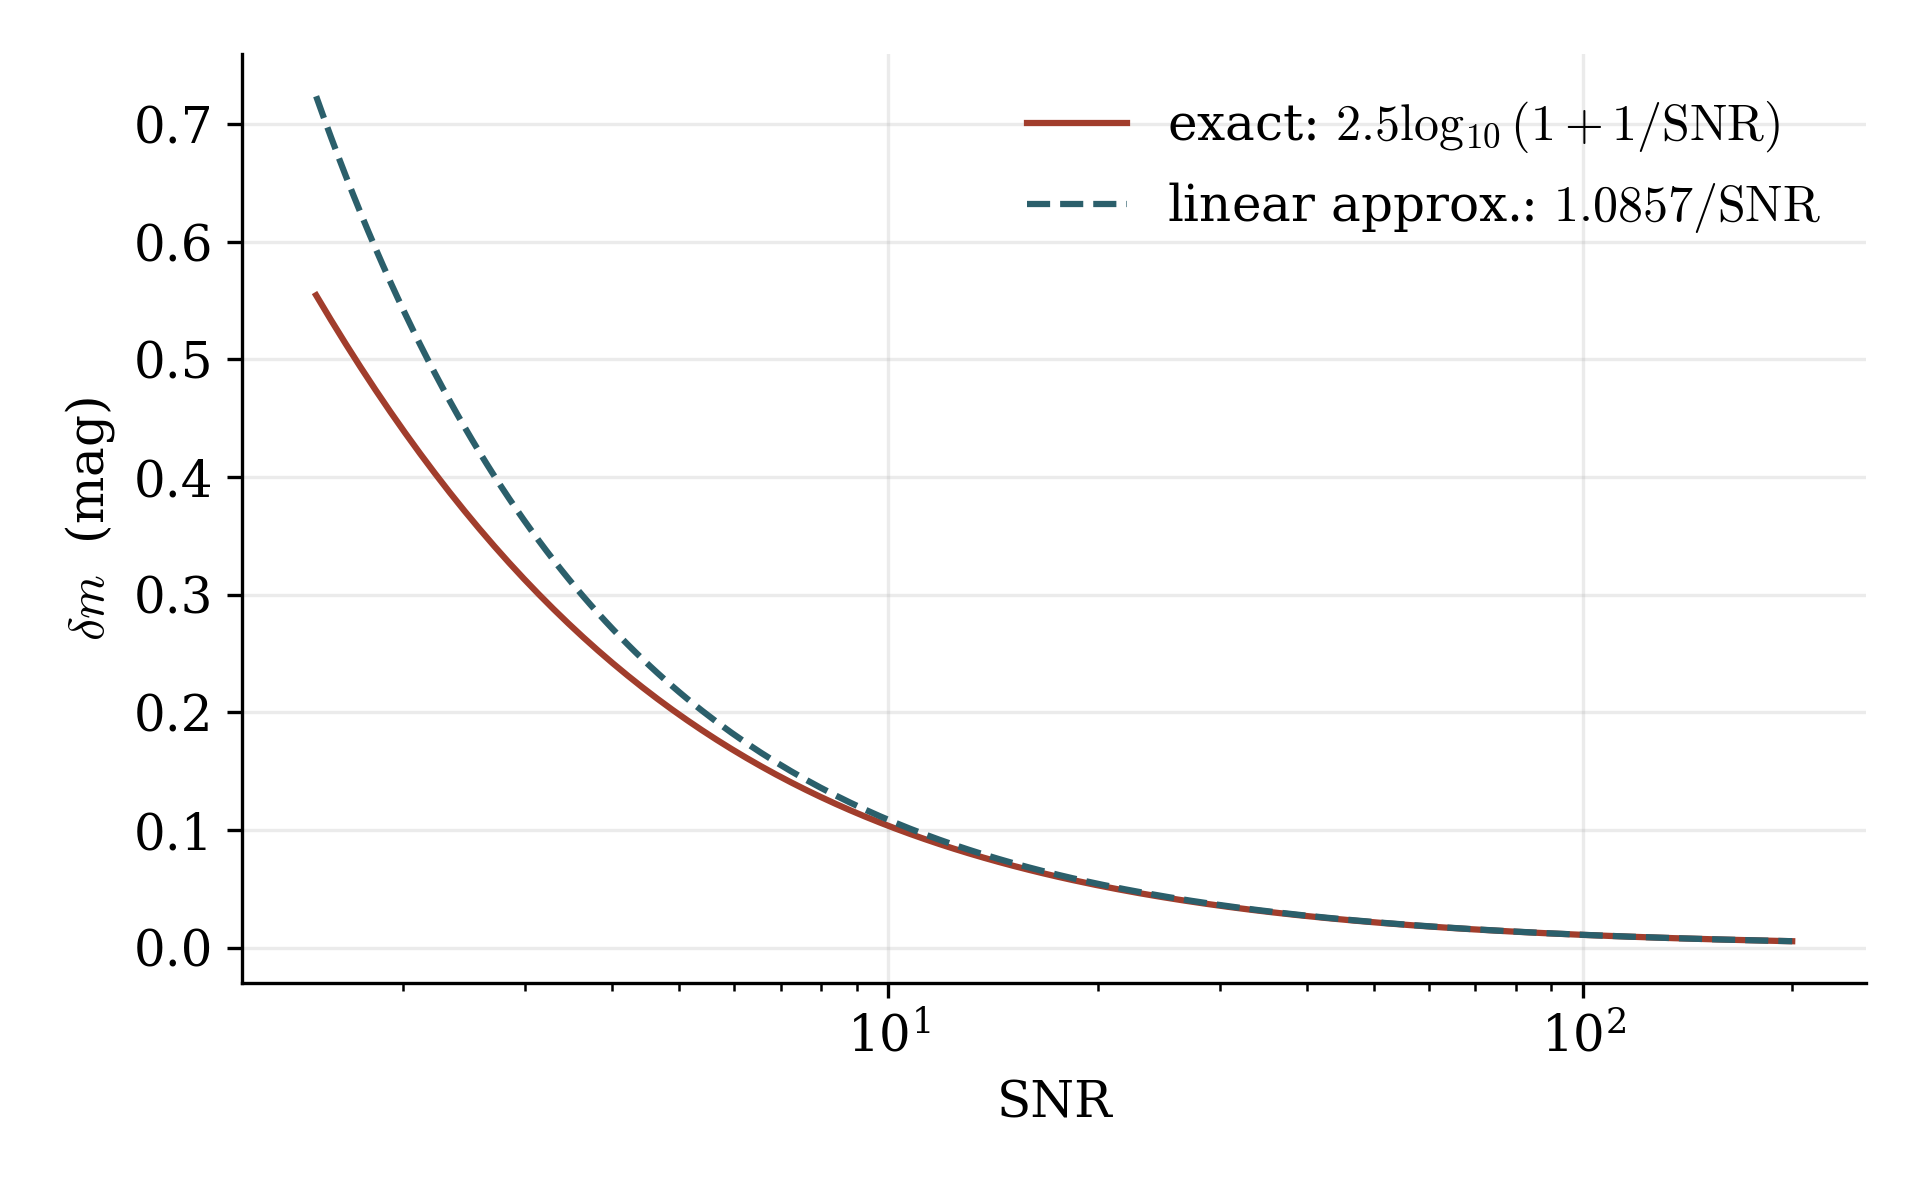
\includegraphics[width=0.72\textwidth]{figs/fig3_dmag.png}
		\caption{Exact photometric magnitude error $\delta m$ compared against the first-order approximation $\delta m \approx 1.0857/\mathrm{SNR}$ as a function of $\mathrm{SNR}$. The curves converge above $\mathrm{SNR}\sim 10$ and diverge significantly below $\mathrm{SNR}\sim 5$.}
		\label{fig:dmag_comparison}
	\end{figure}

	\subsection{Detection Significance and the False-Alarm Probability}

	At the low-SNR threshold ($\mathrm{SNR} = 2\text{--}5$), the central question is whether an observed signal corresponds to a genuine astrophysical source or merely an extreme statistical fluctuation of the background.

	\paragraph{Gaussian Noise Assumption via the Central Limit Theorem.}
	Because the total detected electron count is the sum of many independent Poisson-distributed quantum events and amplifier readouts across multiple pixels, the Central Limit Theorem guarantees that the distribution of total noise $\sigma_{\rm tot}$ is exceedingly well approximated by a Gaussian (normal) distribution $\mathcal{N}(0, \sigma_{\rm tot}^2)$. This justifies expressing detection thresholds in units of standard deviations ($k\sigma$).

	In the null hypothesis (where no astronomical source is present, $S=0$), the probability that pure background noise fluctuates upward by at least $k\sigma_{\rm tot}$ is given by the complementary standard normal cumulative distribution function (Gaussian upper tail):
	\begin{keyresult}
		\begin{equation}
			P(k) = \int_{k}^{\infty} \frac{1}{\sqrt{2\pi}} e^{-x^2/2}\,dx = 1 - \Phi(k).
			\label{eq:false_alarm_single}
		\end{equation}
	\end{keyresult}

	\begin{tcolorbox}[notebox, title=NUMERICAL EVALUATION OF FALSE-ALARM PROBABILITIES]
		Evaluating the Gaussian tail integral numerically:
		\begin{itemize}
			\item $k = 2\sigma$: $P(2) = 2.28 \times 10^{-2}$ ($\sim 1 \text{ in } 44$)
			\item $k = 3\sigma$: $P(3) = 1.35 \times 10^{-3}$ ($\sim 1 \text{ in } 741$)
			\item $k = 5\sigma$: $P(5) = 2.87 \times 10^{-7}$ ($\sim 1 \text{ in } 3.48 \text{ million}$)
			\item $k = 10\sigma$: $P(10) = 7.62 \times 10^{-24}$ ($\sim \text{physically impossible by pure chance}$)
		\end{itemize}
		The steep exponential decline of false-alarm probability with increasing significance is plotted in Figure~\ref{fig:gaussian_tail_prob}.
	\end{tcolorbox}

	\begin{figure}[htbp]
		\centering
		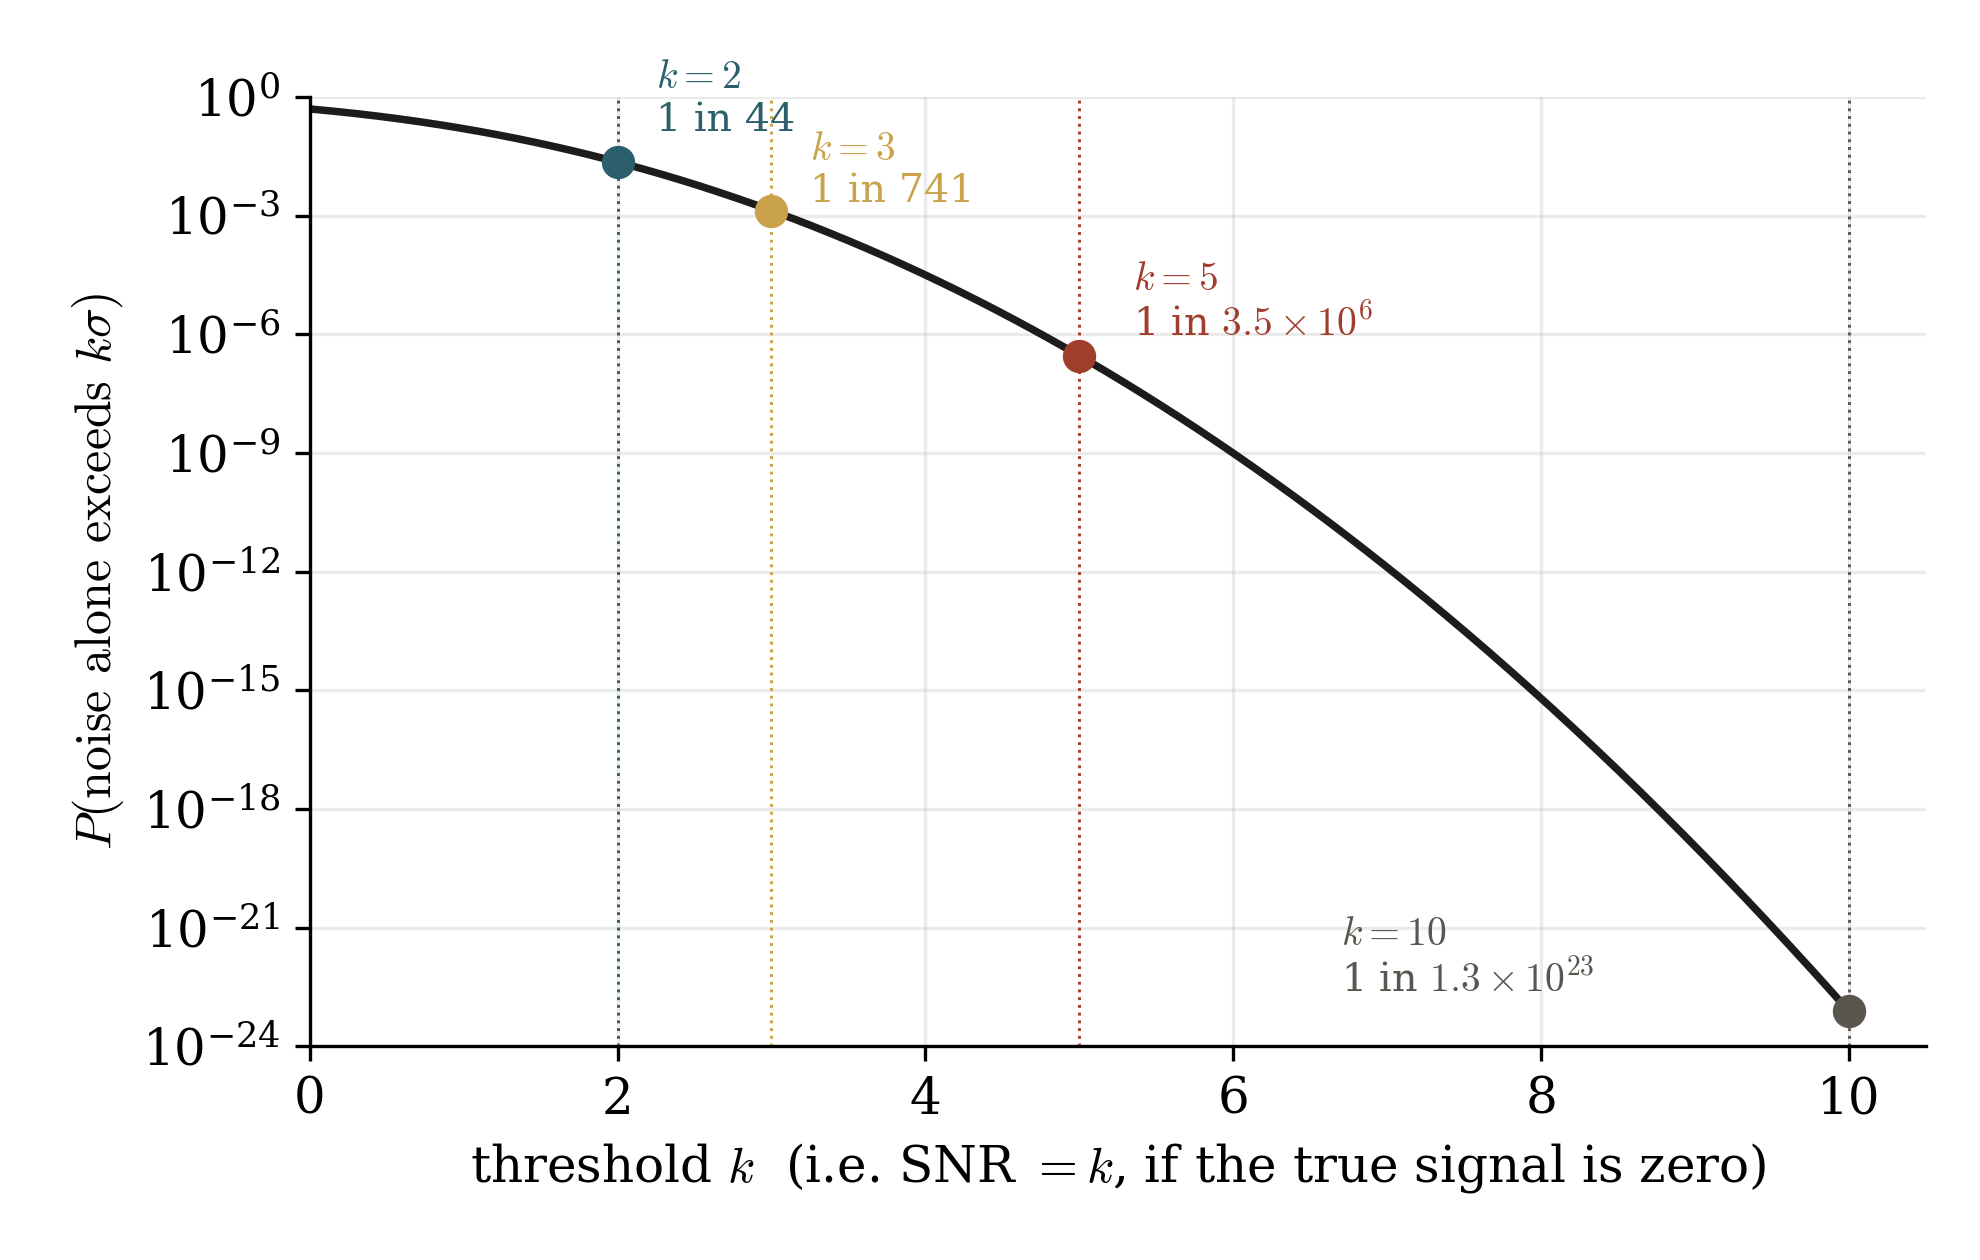
\includegraphics[width=0.72\textwidth]{figs/fig_gaussian_tail.png}
		\caption{Single-trial false-alarm probability $P(k)$ that zero-mean Gaussian background noise generates an apparent excess exceeding $k\sigma$, plotted on a logarithmic scale.}
		\label{fig:gaussian_tail_prob}
	\end{figure}

	\subsection{The Look-Elsewhere Effect and Multi-Pixel Detection Thresholds}

	The single-trial probability $P(k)$ applies when evaluating a pre-specified location (e.g., measuring the flux of a known target star). However, in wide-field blind searches (transient detection, asteroid searches, survey discovery), one tests $n_{\rm trial}$ independent resolution elements simultaneously.

	\begin{tcolorbox}[flagbox, title=THE CATCH: FALSE ALARMS SCALE WITH SEARCH VOLUME]
		If an image contains $n_{\rm trial}$ independent apertures or resolution elements, the probability that \emph{at least one} pure-noise fluctuation exceeds $k\sigma$ is bounded by the union bound:
		\begin{equation}
			P_{\rm any}(k) \approx n_{\rm trial}\,P(k).
			\label{eq:union_bound}
		\end{equation}
		For a modern $4000 \times 4000$ CCD detector ($n_{\rm trial} \approx 1.6 \times 10^7$ pixels):
		\begin{itemize}
			\item At $k=3\sigma$: Expected noise false positives $= (1.6 \times 10^7) \times (1.35 \times 10^{-3}) \approx 2.2 \times 10^4$ spurious detections! The survey is hopelessly swamped by artifacts.
			\item At $k=5\sigma$: Expected noise false positives $= (1.6 \times 10^7) \times (2.87 \times 10^{-7}) \approx 4.6$ false detections across the entire mosaic.
			\item At $k \ge 5.5\sigma$: Expected noise false positives $< 0.3$, guaranteeing that any candidate is almost certainly real.
		\end{itemize}
		This explains why large-scale astronomical surveys universally enforce a $5\sigma$ threshold for discovery claims.
	\end{tcolorbox}

	\section{Physical Origins of Noise in CCD Measurements}

	The total uncertainty $\sigma_{\rm tot}$ is not a monolithic quantity. It is the quadrature sum of four physically distinct processes: photon shot noise from the source, shot noise from the sky background, shot noise from thermal dark current, and readout noise from on-chip amplifiers.

	\subsection{First-Principles Derivation of Photon Shot Noise}

	Even if an astronomical source emits at a perfectly steady mean luminosity, the number of photoelectrons collected in consecutive equal intervals fluctuates. This fundamental variance arises because electromagnetic radiation is quantized: photons arrive as discrete, independent packets.

	\paragraph{Derivation from the Binomial Distribution.}
	Let photons arrive at a constant average rate $\lambda$ (photons per second). Divide the exposure time $t$ into $N$ infinitesimal time bins of duration $\Delta t = t/N$. In each subinterval, the probability of detecting a single photon is $p = \lambda\Delta t = \mu/N$ (where $\mu = \lambda t$ is the expected total count), while the probability of multiple arrivals in the same subinterval approaches zero as $N \to \infty$.

	Because the arrival in each subinterval is an independent Bernoulli trial, the probability of obtaining exactly $n$ arrivals in $N$ subintervals follows the Binomial distribution:
	\begin{equation}
		P(n) = \binom{N}{n} p^n (1-p)^{N-n} = \frac{N!}{n!(N-n)!}\left(\frac{\mu}{N}\right)^n \left(1 - \frac{\mu}{N}\right)^{N-n}.
	\end{equation}
	Taking the continuous limit $N \to \infty$ with $\mu$ held fixed, using $\frac{N!}{(N-n)!N^n} \to 1$ and $(1 - \mu/N)^N \to e^{-\mu}$, we recover the \emph{Poisson distribution}:
	\begin{keyresult}
		\begin{equation}
			P(n;\mu) = \frac{\mu^n e^{-\mu}}{n!}.
			\label{eq:poisson_dist}
		\end{equation}
	\end{keyresult}

	\paragraph{Derivation of Mean and Variance.}
	The expectation value of $n$ is:
	\begin{equation}
		\langle n \rangle = \sum_{n=0}^{\infty} n\,\frac{\mu^n e^{-\mu}}{n!} = \mu e^{-\mu}\sum_{n=1}^{\infty} \frac{\mu^{n-1}}{(n-1)!} = \mu e^{-\mu} e^{\mu} = \mu.
		\label{eq:poisson_mean}
	\end{equation}
	Evaluating the second factorial moment $\langle n(n-1)\rangle$:
	\begin{equation}
		\langle n(n-1) \rangle = \sum_{n=0}^{\infty} n(n-1)\,\frac{\mu^n e^{-\mu}}{n!} = \mu^2 e^{-\mu}\sum_{n=2}^{\infty}\frac{\mu^{n-2}}{(n-2)!} = \mu^2 e^{-\mu} e^{\mu} = \mu^2.
	\end{equation}
	Since $\langle n^2 \rangle = \langle n(n-1)\rangle + \langle n\rangle = \mu^2 + \mu$, the variance is:
	\begin{equation}
		\mathrm{Var}(n) = \langle n^2 \rangle - \langle n\rangle^2 = (\mu^2 + \mu) - \mu^2 = \mu.
		\label{eq:poisson_var}
	\end{equation}
	The standard deviation (shot noise) is therefore:
	\begin{keyresult}
		\begin{equation}
			\sigma = \sqrt{\mathrm{Var}(n)} = \sqrt{\mu}.
			\label{eq:shot_noise_sigma}
		\end{equation}
	\end{keyresult}

	\begin{tcolorbox}[notebox, title=CHECKED NUMERICALLY]
		For $\mu=10$, summing Eq.~\eqref{eq:poisson_dist} directly (truncated at $n=200$) gives $\sum_n P(n)=1.0000$, $\langle n\rangle = 10.000$, and $\mathrm{Var}(n)=10.000$ --- confirming the analytical results.
	\end{tcolorbox}

	\begin{figure}[htbp]
		\centering
		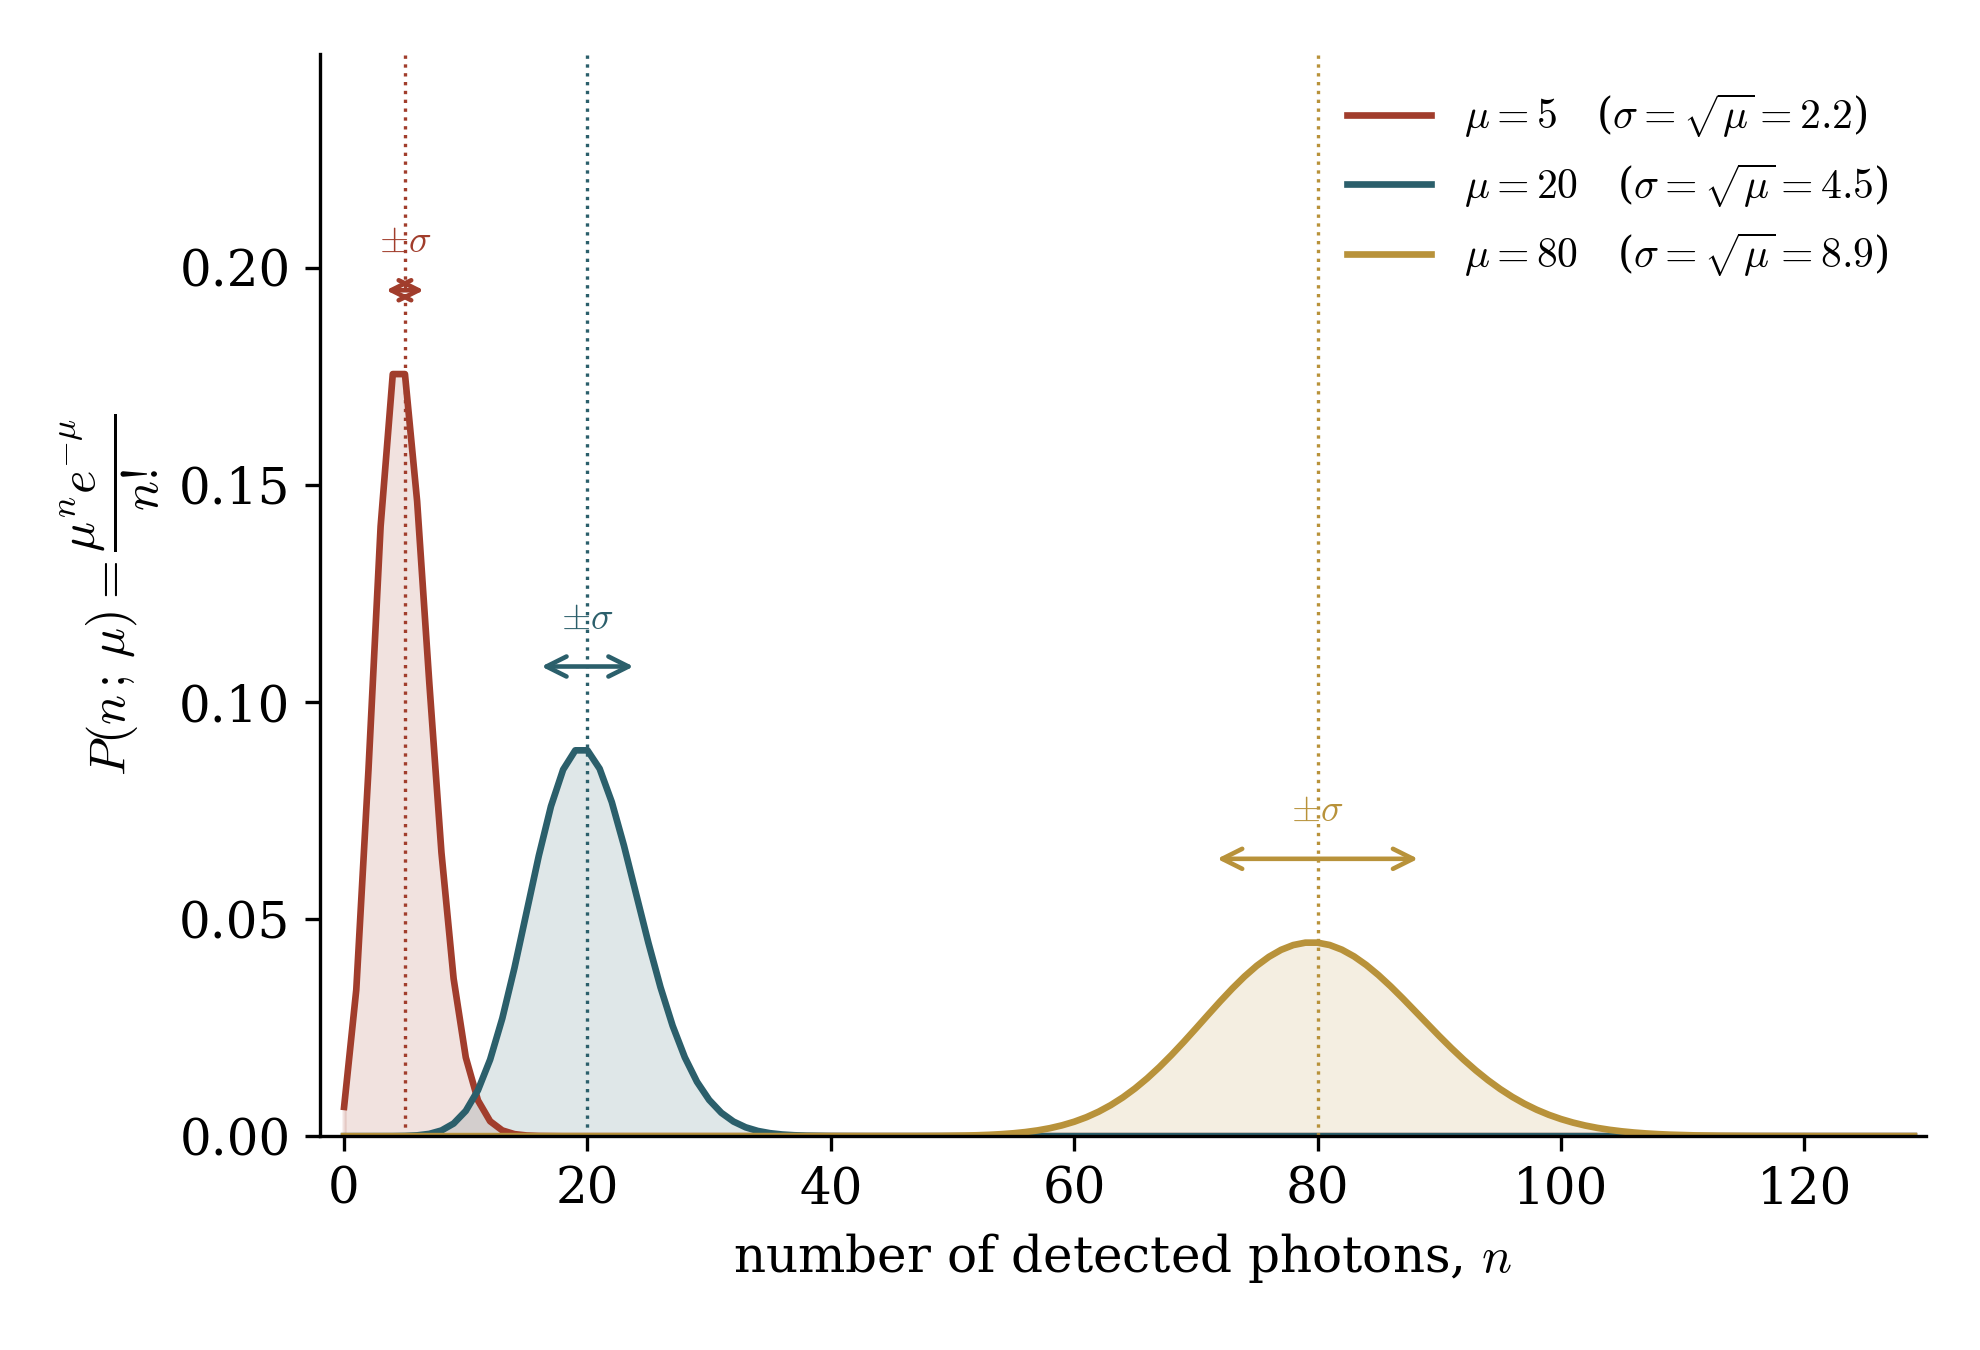
\includegraphics[width=0.82\textwidth]{figs/fig0_poisson.png}
		\caption{The Poisson probability distribution $P(n;\mu)$ for mean counts $\mu = 10, 50, 250$. While the absolute standard deviation $\sigma = \sqrt{\mu}$ grows with brightness, the relative fractional noise $\sigma/\mu = 1/\sqrt{\mu}$ contracts, leading directly to the $\mathrm{SNR} \propto \sqrt{\mu}$ scaling of photon-limited measurements.}
		\label{fig:poisson_distributions}
	\end{figure}

	\subsection{The Three Counting Shot-Noise Contributions}

	Applying Eq.~\eqref{eq:shot_noise_sigma} to each independent physical source of photoelectrons:

	\begin{enumerate}
		\item \textbf{Object Shot Noise:} The astronomical source delivers $S = R_{\rm src}t$ photoelectrons inside the aperture, giving:
		\begin{equation}
			\sigma_{\rm src} = \sqrt{S} = \sqrt{R_{\rm src}\,t}.
			\label{eq:sigma_src}
		\end{equation}

		\item \textbf{Sky Background Shot Noise:} The sky background emits photons uniformly across the focal plane at rate $R_{\rm sky}$ per pixel. Over an aperture of $n_{\rm pix}$ pixels during exposure $t$, the accumulated sky electrons are $n_{\rm pix}R_{\rm sky}t$. Although the mean sky level is subtracted during data reduction, its Poisson fluctuation remains:
		\begin{equation}
			\sigma_{\rm sky} = \sqrt{n_{\rm pix}\,R_{\rm sky}\,t}.
			\label{eq:sigma_sky}
		\end{equation}
		Because the required photometric aperture area scales with seeing disk size ($n_{\rm pix} \propto \theta_{\rm see}^2$), superior seeing directly reduces sky noise.

		\item \textbf{Dark Current Shot Noise:} Thermal vibrations in the silicon lattice spontaneously generate electron-hole pairs at rate $R_{\rm dark}$ per pixel. These accumulate over $n_{\rm pix}$ pixels and duration $t$:
		\begin{equation}
			\sigma_{\rm dark} = \sqrt{n_{\rm pix}\,R_{\rm dark}\,t}.
			\label{eq:sigma_dark}
		\end{equation}
	\end{enumerate}

	\begin{tcolorbox}[flagbox, title=UNITS CAUTION: DARK CURRENT CONVERSIONS]
		Manufacturers and detector manuals frequently quote dark current in units of $\mathrm{e^-\,pixel^{-1}\,hr^{-1}}$. When inserting $R_{\rm dark}$ into Eq.~\eqref{eq:sigma_dark} with exposure time $t$ in seconds, $R_{\rm dark}$ must be converted to $\mathrm{e^-\,s^{-1}\,pix^{-1}}$:
		\[
		R_{\rm dark}\,[\mathrm{e^-\,s^{-1}\,pix^{-1}}] = \frac{R_{\rm dark}\,[\mathrm{e^-\,hr^{-1}\,pix^{-1}}]}{3600\,\mathrm{s/hr}}.
		\]
		Throughout these notes, all rates ($R_{\rm src}, R_{\rm sky}, R_{\rm dark}$) are strictly in $\mathrm{e^-\,s^{-1}}$.
	\end{tcolorbox}

	\subsection{Readout Noise: The Additive Amplifier Penalty}

	Unlike the three counting processes above, readout noise is \emph{not} a shot noise. It arises from thermal (Johnson-Nyquist) and flicker ($1/f$) electronic noise in the output field-effect transistor (FET) and analog-to-digital converter (ADC) during charge-to-voltage conversion.

	Readout noise adds a constant Gaussian uncertainty $\sigma_{\rm RON}$ (in electrons RMS) to each pixel per readout, independent of exposure time. For $n_{\rm pix}$ pixels read out in each of $N_{\rm exp}$ independent exposures:
	\begin{keyresult}
		\begin{equation}
			\sigma_{\rm read} = \sqrt{n_{\rm pix}\,N_{\rm exp}}\;\sigma_{\rm RON}.
			\label{eq:sigma_read}
		\end{equation}
	\end{keyresult}
	Note the fundamental structural difference: $\sigma_{\rm read}^2 \propto N_{\rm exp}$ rather than $\propto t$. Splitting an exposure of duration $t$ into $N_{\rm exp}$ shorter exposures incurs the read noise penalty $N_{\rm exp}$ times in variance.

	\section{The Master Signal-to-Noise Ratio Equation}

	\begin{tcolorbox}[notebox, title=FIRST-PRINCIPLES DERIVATION: WHY VARIANCES ADD FOR INDEPENDENT NOISE SOURCES]
		Let $X$ and $Y$ be two random variables representing independent physical noise processes with expected values $\mu_X = \mathbb{E}[X]$, $\mu_Y = \mathbb{E}[Y]$ and variances $\sigma_X^2 = \mathrm{Var}(X)$, $\sigma_Y^2 = \mathrm{Var}(Y)$.

		The variance of their sum $Z = X + Y$ is defined by:
		\begin{equation}
			\mathrm{Var}(X + Y) = \mathbb{E}\left[\big((X + Y) - \mathbb{E}[X + Y]\big)^2\right] = \mathbb{E}\left[\big((X - \mu_X) + (Y - \mu_Y)\big)^2\right].
		\end{equation}
		Expanding the algebraic square inside the expectation:
		\begin{equation}
			\big((X - \mu_X) + (Y - \mu_Y)\big)^2 = (X - \mu_X)^2 + (Y - \mu_Y)^2 + 2(X - \mu_X)(Y - \mu_Y).
		\end{equation}
		Applying the linearity of the mathematical expectation operator $\mathbb{E}[\,\cdot\,]$:
		\begin{align}
			\mathrm{Var}(X + Y) &= \mathbb{E}\left[(X - \mu_X)^2\right] + \mathbb{E}\left[(Y - \mu_Y)^2\right] + 2\,\mathbb{E}\left[(X - \mu_X)(Y - \mu_Y)\right] \notag \\
			&= \mathrm{Var}(X) + \mathrm{Var}(Y) + 2\,\mathrm{Cov}(X, Y).
		\end{align}
		Because the physical mechanisms generating astronomical source photons, sky background photons, thermal dark current, and amplifier readout noise are statistically \emph{independent}, their joint probability density factorizes: $p(x, y) = p_X(x)\,p_Y(y)$. The covariance therefore vanishes identically:
		\begin{equation}
			\mathrm{Cov}(X, Y) = \mathbb{E}[(X - \mu_X)]\,\mathbb{E}[(Y - \mu_Y)] = 0 \cdot 0 = 0.
		\end{equation}
		By mathematical induction, for $N$ mutually independent noise contributions $X_1, X_2, \dots, X_N$:
		\begin{equation}
			\mathrm{Var}\left(\sum_{i=1}^N X_i\right) = \sum_{i=1}^N \mathrm{Var}(X_i) \quad\Longrightarrow\quad \sigma_{\rm tot}^2 = \sum_{i=1}^N \sigma_i^2 \quad\Longleftrightarrow\quad \sigma_{\rm tot} = \sqrt{\sum_{i=1}^N \sigma_i^2}.
		\end{equation}
		This rigorous result proves why independent noise contributions must be added in quadrature, establishing the fundamental basis of the CCD noise budget.
	\end{tcolorbox}

	Because the four noise sources arise from statistically independent physical mechanisms, their variances add in quadrature:
	\begin{equation}
		\sigma_{\rm tot}^2 = \sigma_{\rm src}^2 + \sigma_{\rm sky}^2 + \sigma_{\rm dark}^2 + \sigma_{\rm read}^2.
		\label{eq:variance_addition}
	\end{equation}
	Substituting the derived expressions into Eq.~\eqref{eq:snr_def} yields the \textbf{Master CCD Signal-to-Noise Equation}:

	\begin{tcolorbox}[enhanced, colback=white, colframe=ink, boxrule=0.9pt, arc=0pt, left=14pt, right=14pt, top=10pt, bottom=10pt]
		\begin{equation}
			\mathrm{SNR} = \frac{R_{\rm src}\,t}{\sqrt{R_{\rm src}\,t \;+\; n_{\rm pix}R_{\rm sky}\,t \;+\; n_{\rm pix}R_{\rm dark}\,t \;+\; n_{\rm pix}N_{\rm exp}\,\sigma_{\rm RON}^2}}
			\label{eq:master_ccd_snr}
		\end{equation}
	\end{tcolorbox}
	where $t = N_{\rm exp}t_{\rm exp}$. This single equation governs all exposure time calculators (ETCs) in observational astronomy.

	\begin{figure}[htbp]
		\centering
		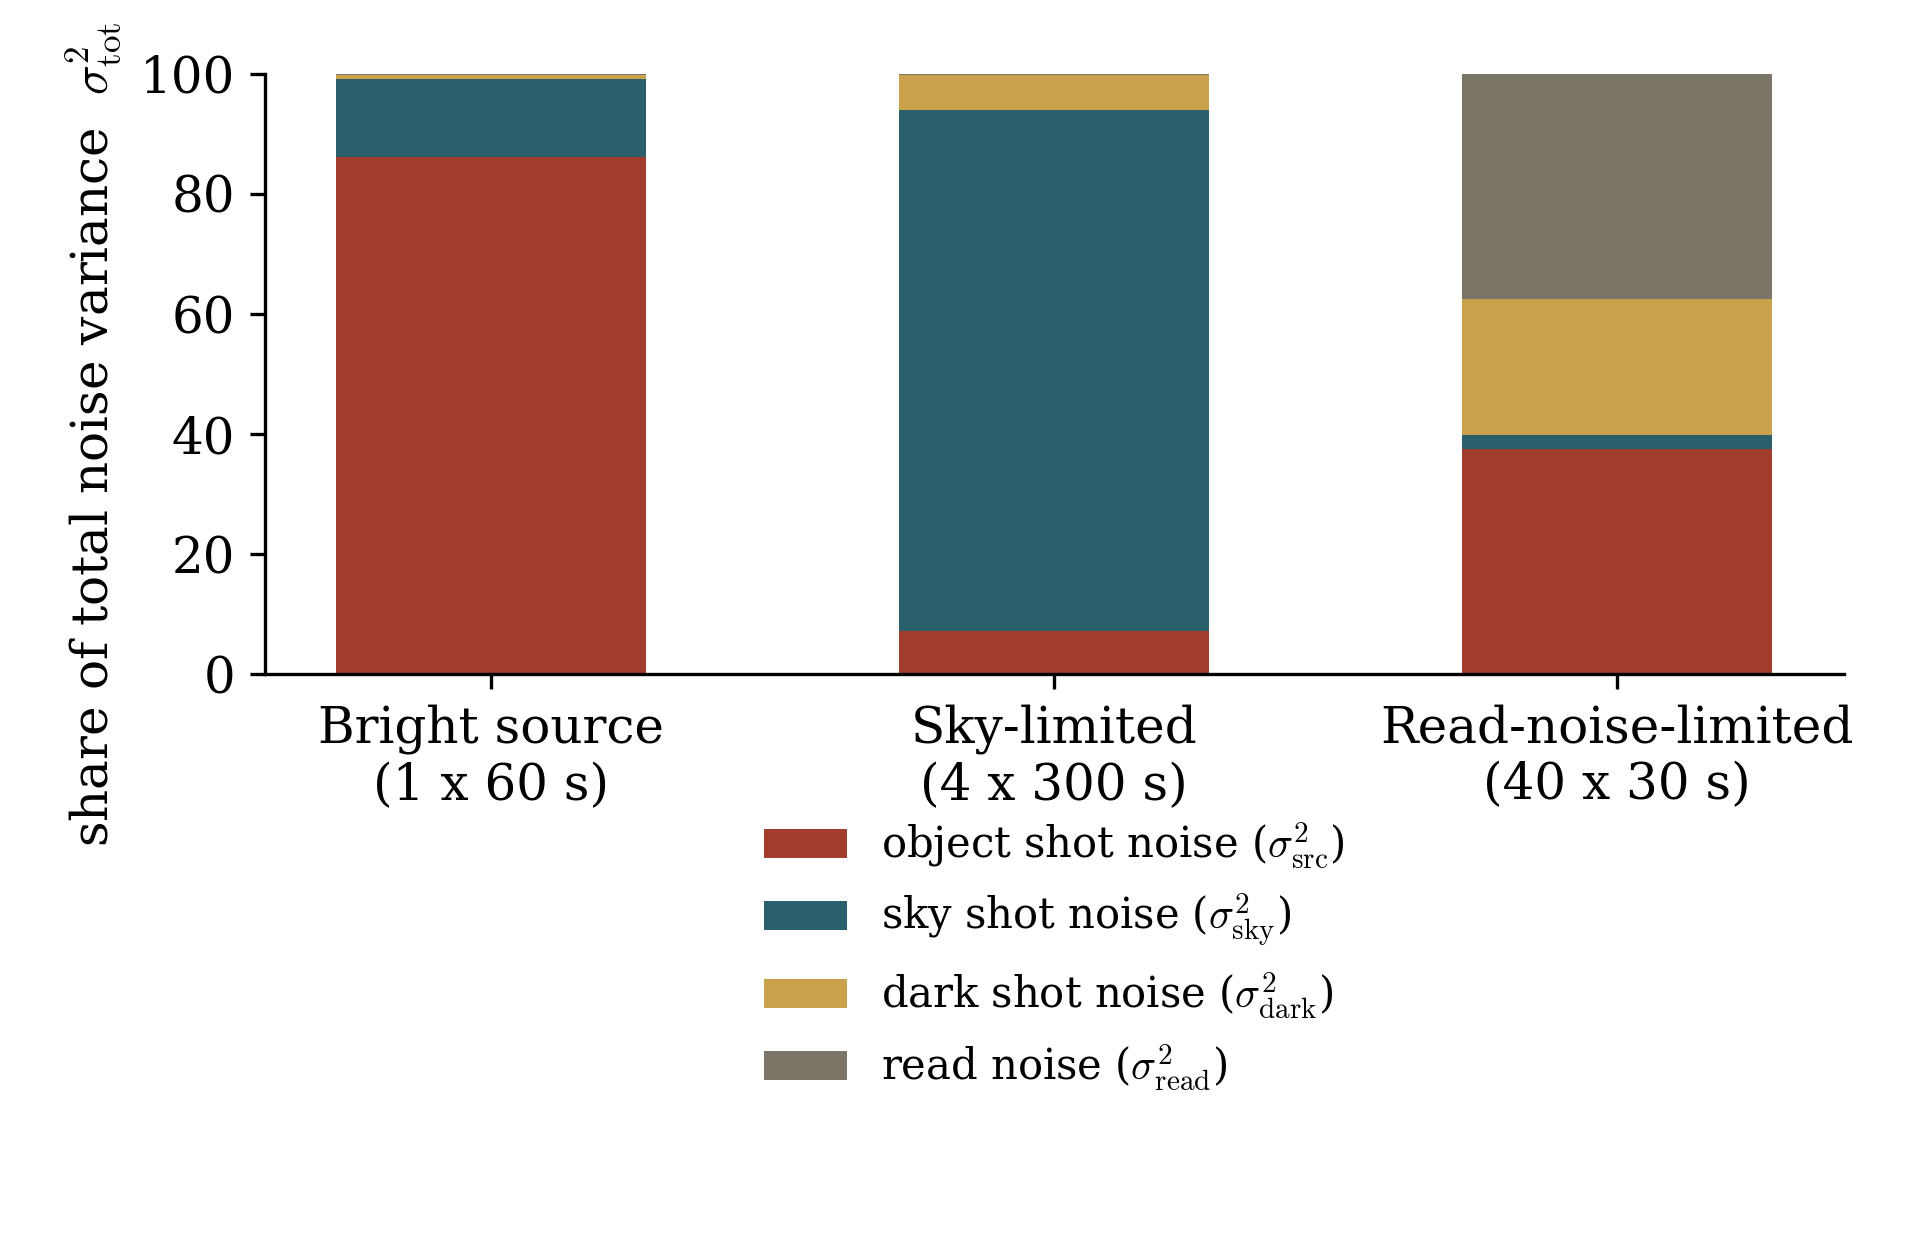
\includegraphics[width=0.85\textwidth]{figs/fig1_budget.png}
		\caption{Relative variance budget ($\sigma_i^2/\sigma_{\rm tot}^2 \times 100\%$) across three characteristic observational scenarios. Identifying which variance component dominates dictates the optimal observational strategy.}
		\label{fig:noise_budget}
	\end{figure}

	\section{The Three Observational Regimes and Exposure Planning Strategies}

	Depending on target flux, background brightness, and detector characteristics, the master equation simplifies into three distinct physical regimes.

	\subsection{Regime 1: Bright Source (Photon Shot-Noise Limited)}
	When observing a bright star, the source count rate dominates over sky, dark current, and read noise ($R_{\rm src}t \gg n_{\rm pix}(R_{\rm sky} + R_{\rm dark})t + n_{\rm pix}N_{\rm exp}\sigma_{\rm RON}^2$):
	\begin{keyresult}
		\begin{equation}
			\mathrm{SNR} \approx \frac{R_{\rm src}t}{\sqrt{R_{\rm src}t}} = \sqrt{R_{\rm src}t} \propto \sqrt{t}.
			\label{eq:regime_bright}
		\end{equation}
	\end{keyresult}
	\paragraph{Observational Strategy.} The limitation in this regime is never achieving adequate $\mathrm{SNR}$, but avoiding detector saturation (full-well capacity, typically $\sim 10^5\,\mathrm{e^-/pixel}$) and non-linear response. Observers should shorten $t_{\rm exp}$ or defocus the telescope (spread light over more pixels) to prevent saturation while accumulating the desired total photon count.

	\subsection{Regime 2: Sky-Background Limited}
	For faint targets observed in broadband optical filters, the night sky background is much brighter than the source ($n_{\rm pix}R_{\rm sky}t \gg R_{\rm src}t, n_{\rm pix}R_{\rm dark}t, n_{\rm pix}N_{\rm exp}\sigma_{\rm RON}^2$):
	\begin{keyresult}
		\begin{equation}
			\mathrm{SNR} \approx \frac{R_{\rm src}t}{\sqrt{n_{\rm pix}R_{\rm sky}t}} = \frac{R_{\rm src}\sqrt{t}}{\sqrt{n_{\rm pix}R_{\rm sky}}} \propto \frac{\sqrt{t}}{\sqrt{n_{\rm pix}}}.
			\label{eq:regime_sky}
		\end{equation}
	\end{keyresult}
	\paragraph{Observational Strategies.}
	\begin{itemize}
		\item \textbf{Seeing is paramount:} Because $n_{\rm pix} \propto \theta_{\rm see}^2$, the signal-to-noise ratio scales as $\mathrm{SNR} \propto 1/\theta_{\rm see}$. Improving seeing from $1.2''$ to $0.6''$ doubles the $\mathrm{SNR}$ (equivalent to a factor of 4 reduction in required telescope integration time).
		\item \textbf{Sub-exposure splitting is free:} In this regime, $\mathrm{SNR}$ depends strictly on total integration time $t$, not on the number of frames $N_{\rm exp}$. Splitting a $3000\,\mathrm{s}$ integration into ten $300\,\mathrm{s}$ frames incurs negligible read-noise penalty while enabling robust cosmic-ray rejection, dithering to remove bad pixels, and dynamic range preservation.
	\end{itemize}

	\subsection{Regime 3: Readout-Noise Limited}
	When observing faint objects under low background levels (narrow-band filters, high-resolution spectroscopy, or very short exposures), the readout noise dominates ($n_{\rm pix}N_{\rm exp}\sigma_{\rm RON}^2 \gg (R_{\rm src} + n_{\rm pix}R_{\rm sky} + n_{\rm pix}R_{\rm dark})t$):
	\begin{keyresult}
		\begin{equation}
			\mathrm{SNR} \approx \frac{R_{\rm src}t}{\sqrt{n_{\rm pix}N_{\rm exp}}\,\sigma_{\rm RON}} \propto \frac{1}{\sqrt{n_{\rm pix}}}\cdot\frac{1}{\sqrt{N_{\rm exp}}}.
			\label{eq:regime_read}
		\end{equation}
	\end{keyresult}
	\paragraph{Observational Strategies.}
	\begin{itemize}
		\item \textbf{On-Chip Pixel Binning:} Binning pixels on-chip (e.g., $2\times 2$) combines charges in the shift registers before readout, reducing the effective $n_{\rm pix}$ by a factor of 4 and boosting $\mathrm{SNR}$ by $\sqrt{4} = 2$ without increasing read noise. Binning should be applied up to the Nyquist limit ($\sim 2\text{--}3$ binned pixels across the seeing FWHM or resolution element).
		\item \textbf{Maximize Individual Exposure Duration:} Because $\mathrm{SNR} \propto 1/\sqrt{N_{\rm exp}}$ at fixed total time $t$, one should make $t_{\rm exp}$ as long as possible (minimizing $N_{\rm exp}$). The maximum safe exposure length is typically limited by cosmic-ray hit density ($\sim 30\text{--}45\,\mathrm{min}$ for ground-based CCDs).
	\end{itemize}

	\begin{figure}[htbp]
		\centering
		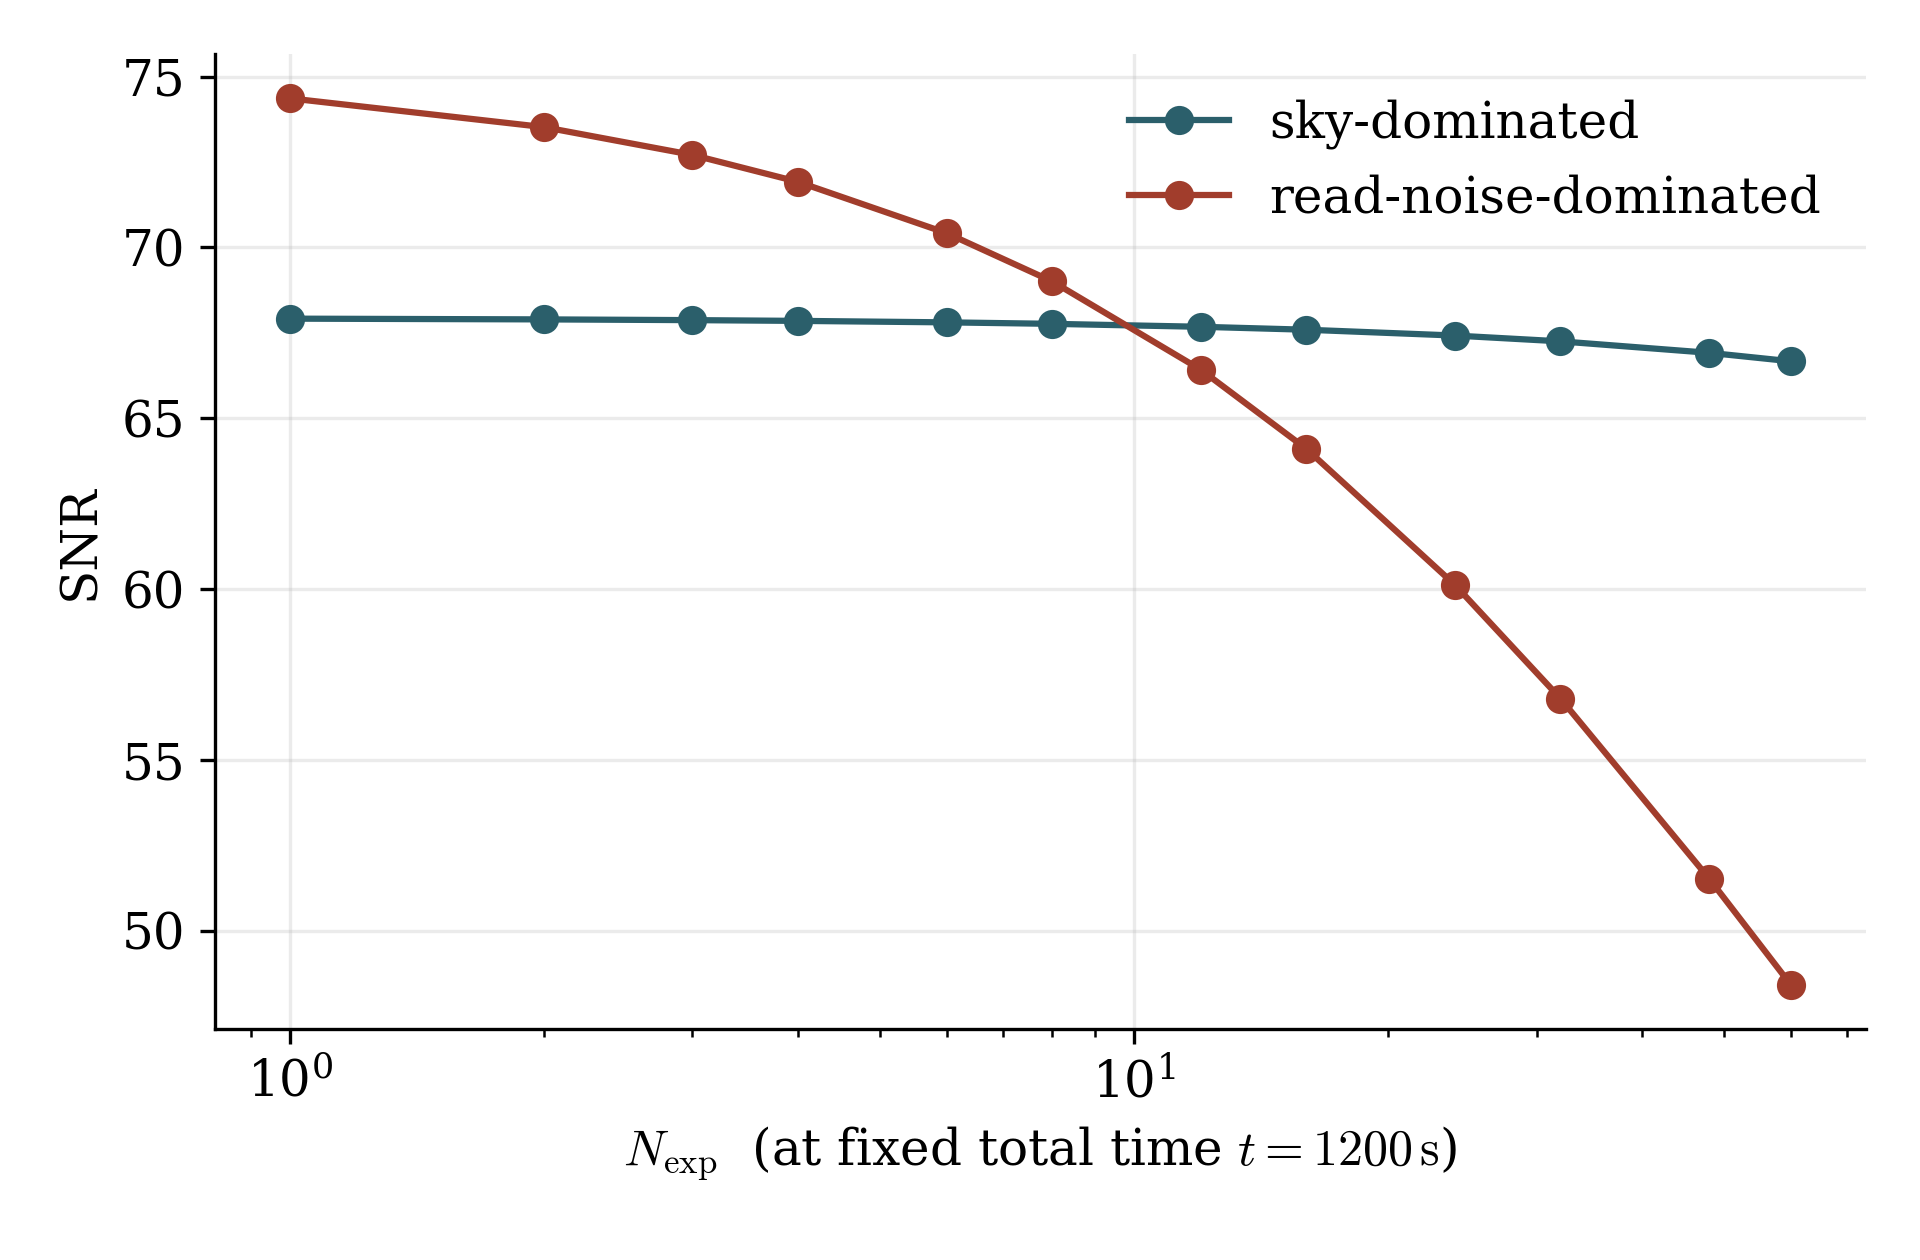
\includegraphics[width=0.85\textwidth]{figs/fig2_nexp.png}
		\caption{Signal-to-noise ratio as a function of the number of sub-exposures $N_{\rm exp}$ at fixed total exposure time $t = 1200\,\mathrm{s}$. In the sky-limited regime, the curve is virtually flat, making exposure splitting cost-free. In the read-noise-limited regime, each additional readout adds an unrecoverable noise penalty, degrading $\mathrm{SNR}$.}
		\label{fig:nexp_comparison}
	\end{figure}

	\section{Summary and Observational Decision Matrix}

	All photometric noise trade-offs are governed by which term in the variance sum $\sigma_{\rm tot}^2$ dominates. Table~\ref{tab:regime_summary} provides an operational decision matrix for planning astronomical exposures.

	\begin{table}[htbp]
		\centering
		\begin{tabular}{@{}l l l p{6.2cm}@{}}
			\toprule
			\textbf{Regime} & \textbf{Dominant Variance} & \textbf{SNR Scaling} & \textbf{Operational Strategy} \\
			\midrule
			Bright Source & $\sigma_{\rm src}^2 = R_{\rm src}t$ & $\mathrm{SNR} \propto \sqrt{t}$ & Monitor full-well capacity; prevent saturation and non-linearity. \\
			\addlinespace[0.4em]
			Sky-Limited & $\sigma_{\rm sky}^2 = n_{\rm pix}R_{\rm sky}t$ & $\mathrm{SNR} \propto \dfrac{\sqrt{t}}{\sqrt{n_{\rm pix}}}$ & Minimize aperture (exploit good seeing); freely split into $N_{\rm exp}$ sub-exposures for CR rejection. \\
			\addlinespace[0.4em]
			Read-Noise Limited & $\sigma_{\rm read}^2 = n_{\rm pix}N_{\rm exp}\sigma_{\rm RON}^2$ & $\mathrm{SNR} \propto \dfrac{1}{\sqrt{n_{\rm pix}N_{\rm exp}}}$ & Bin pixels on-chip (up to Nyquist sampling); maximize $t_{\rm exp}$ (minimize $N_{\rm exp}$) within CR limits. \\
			\bottomrule
		\end{tabular}
		\caption{Comparative overview of the three observational regimes, dominant noise terms, signal-to-noise scalings, and observing strategies.}
		\label{tab:regime_summary}
	\end{table}

	\FloatBarrier

\end{document}

\chapter{The Interstellar Medium and Gravitational Collapse}

Chapters~1--7 treated a star (or a pulsar, or a binary) essentially as an isolated point source: a clock, a moving mass, a blackbody, a photon-emitting aperture problem. In reality, no photon reaches a telescope without first traversing tens to thousands of parsecs of gas and dust --- the \emph{interstellar medium} (ISM). The ISM scatters, absorbs, and disperses the light we use for every measurement in this book, and it is also the raw material out of which every star is born and into which every star eventually returns its processed mass. This chapter first characterizes the ISM as an absorbing, scattering, and line-emitting medium, and then turns to its own internal dynamics: the virial theorem, the Jeans criterion for gravitational instability, and the free-fall collapse that marks the transition from a diffuse cloud to a forming protostar.

\section{Composition, Density, and Temperature}

\begin{definition}[Interstellar Medium]
	The \emph{interstellar medium} is the matter --- gas, dust, cosmic rays, and magnetic field --- occupying the space between stars within a galaxy.
\end{definition}

Despite containing roughly $20\%$ of the ordinary (baryonic) mass of the Milky Way, the ISM is extraordinarily dilute:

\begin{table}[htbp]
	\centering
	\begin{tabular}{@{}l l@{}}
		\toprule
		\textbf{Property} & \textbf{Typical Value} \\
		\midrule
		Number density $n$ & $10^{-4} \text{--} 10^{6}\,\mathrm{cm^{-3}}$ \\
		Temperature $T$ & $10\text{--}10^{6}\,\mathrm{K}$ \\
		Composition (by mass) & $70\%$ H, $28\%$ He, $\lesssim 2\%$ heavier elements \\
		Phase split (by mass) & $99\%$ gas, $1\%$ dust \\
		Magnetic field strength & $\sim 10^{-10}\,\mathrm{T}$ ($\sim 1\,\mu\mathrm{G}$) \\
		\bottomrule
	\end{tabular}
	\caption{Characteristic bulk properties of the interstellar medium.}
	\label{tab:ism_bulk_properties}
\end{table}

For comparison, the best vacuum achievable in a terrestrial laboratory (extreme high vacuum, XHV) reaches $\sim 10^{5}\,\mathrm{cm^{-3}}$: the diffuse phase of the ISM is routinely \emph{more rarefied than our best laboratory vacuum}. This has an important physical consequence exploited throughout this chapter: at such densities, collisional de-excitation is so infrequent that highly forbidden atomic and molecular transitions --- undetectable in any terrestrial spectrometer --- become the dominant, and often only, radiative channel available to interstellar gas (Section~\ref{sec:ism_hydrogen}).

The gas phase consists of ions (e.g.\ $\mathrm{H^+}$, $\mathrm{He^+}$, $\mathrm{He^{2+}}$), free electrons, and molecules (e.g.\ $\mathrm{H_2}$, CO, CN, $\mathrm{H_2O}$, $\mathrm{NH_3}$). The dust phase consists of sub-micron grains ($\sim 1\,\mathrm{nm}$ to $\sim 1\,\mu\mathrm{m}$) of silicates, amorphous carbon, and metals (Fe, Ni), often mantled with ices ($\mathrm{H_2O, NH_3}$). Although dust carries only $1\%$ of the ISM's mass, its large geometric cross-section per unit mass makes it the dominant agent of interstellar extinction (Section~\ref{sec:ism_extinction}) and the primary catalyst for $\mathrm{H_2}$ formation (Section~\ref{sec:ism_hydrogen}).

Studying the ISM matters for three independent reasons: (i) every photon used in Chapters 1--7 is filtered by it, so its optical properties must be understood before extinction and reddening corrections (Chapter~4) can be trusted; (ii) it hosts physical and chemical regimes --- extreme rarefaction, extreme cold, non-equilibrium chemistry --- inaccessible to any laboratory; and (iii) it is both the birthplace and the graveyard of stars, which is the subject of the second half of this chapter.

\section{Radiative Interaction with Dust: Extinction, Scattering, and Reddening}
\label{sec:ism_extinction}

\begin{definition}[Extinction]
	\emph{Extinction} is the total attenuation of light passing through a medium, defined as the sum of true absorption and scattering out of the line of sight:
	\begin{equation}
		\text{Extinction} = \text{Absorption} + \text{Scattering}.
		\label{eq:extinction_decomposition}
	\end{equation}
\end{definition}

Absorption occurs either as sharp line absorption by atoms and molecules, or as broadband continuum absorption by larger dust grains. Scattering off a grain of radius $a$ falls into three regimes depending on the ratio of grain size to wavelength:

\begin{table}[htbp]
	\centering
	\begin{tabular}{@{}l l l l@{}}
		\toprule
		\textbf{Regime} & \textbf{Condition} & \textbf{Cross-section scaling} & \textbf{Physical origin} \\
		\midrule
		Geometric & $a \gg \lambda$ & $\sigma \propto a^2$ & Ray optics; grain blocks its own geometric shadow. \\
		Mie & $a \sim \lambda$ & $\sigma \propto a^3\lambda^{-1}$ & Full electromagnetic (Mie) solution; no closed form. \\
		Rayleigh & $a \ll \lambda$ & $\sigma \propto a^6\lambda^{-4}$ & Grain acts as a driven electric dipole. \\
		\bottomrule
	\end{tabular}
	\caption{Scattering regimes for a spherical grain of radius $a$ illuminated at wavelength $\lambda$.}
	\label{tab:scattering_regimes}
\end{table}

\paragraph{Physical origin of the three regimes.} The geometric limit is simple ray optics: a grain much larger than the wavelength blocks light over its own projected area, $\sigma = \pi a^2$, independent of $\lambda$. The Rayleigh limit is a classical driven-dipole problem: an incident wave of amplitude $E_0$ induces a dipole moment $p = \alpha E_0$ in the grain, with polarizability $\alpha \propto a^3$ (the response of a sub-wavelength dielectric or conducting sphere scales with its volume). This oscillating dipole radiates according to the Larmor formula, $P_{\rm rad} \propto \ddot p^{\,2} \propto \omega^4 p^2$, so the re-radiated power scales as $\omega^4 a^6 E_0^2 \propto a^6/\lambda^4$ (using $\omega = 2\pi c/\lambda$); dividing by the incident intensity $I \propto E_0^2$ gives the scattering cross-section
\begin{keyresult}
	\begin{equation}
		\sigma_{\rm Rayleigh} \propto \frac{a^6}{\lambda^4}.
		\label{eq:rayleigh_scattering_cross_section}
	\end{equation}
\end{keyresult}
This is precisely the same dipole-scattering result invoked in Chapter~5 (Section~\ref{sec:windows}) for air molecules rather than dust grains, and is the microscopic origin of the $\lambda^{-4}$ law responsible for the blue daytime sky. The intermediate Mie regime, by contrast, has no elementary derivation of this kind: the exact solution requires expanding the scattered field in an infinite series of vector spherical harmonics (the Mie series), whose terms do not collapse to a simple power law; the scaling $\sigma \propto a^3\lambda^{-1}$ quoted in Table~\ref{tab:scattering_regimes} is only the effective average behaviour across this transition regime, not a closed-form result.

Interstellar grains ($a \sim 0.01\text{--}1\,\mu\mathrm{m}$) are comparable to or smaller than optical wavelengths, so ISM scattering is generically in the Mie or Rayleigh regime, both of which share the qualitative feature that $\sigma$ \emph{decreases} with increasing $\lambda$. A beam of white starlight passing through a dusty cloud therefore loses blue photons preferentially, emerging both dimmer (extinction) and redder (\emph{interstellar reddening}) than it left the source. This is the microphysical origin of the empirical extinction law $A_V = R_V\,E(B-V)$ with $R_V \approx 3.1$ already introduced in Chapter~4 (Eq.~\eqref{eq:rv_extinction}): the observed $\gamma \sim 1$ power-law is the net effect of averaging over a realistic grain-size distribution straddling the Mie and Rayleigh regimes, rather than a single clean $\lambda^{-4}$ Rayleigh law. A well-known consequence is visible directly in absorption and reflection nebulae: dense dust lanes such as Barnard 68 appear as near-total silhouettes in the optical yet become largely transparent in the infrared (where $a \ll \lambda$ deep in the Rayleigh regime and $\sigma$ is small), while starlight scattered off the dust surrounding the Pleiades produces a blue reflection nebula for the same Rayleigh-type reason that the terrestrial daytime sky is blue.

\section{Spectral Lines: Formation and Broadening}
\label{sec:ism_lines}

Atoms and ions possess only electronic transitions; molecules additionally possess rotational and vibrational transitions, giving them a far richer spectrum. An excited species relaxing spontaneously produces an \emph{emission} line; a cooler foreground species illuminated by a hotter background continuum source produces an \emph{absorption} line. In neither case is the line infinitely sharp — three independent physical mechanisms set its width.

\subsection{Natural Broadening}

By the time-energy uncertainty relation, a state with a finite lifetime $\Delta\tau$ cannot have an arbitrarily sharp energy:
\begin{equation}
	\Delta E\,\Delta\tau \sim \hbar.
	\label{eq:natural_broadening_energy}
\end{equation}
Since $E = h\nu$, this maps directly onto a minimum frequency width
\begin{equation}
	\Delta\nu_{\rm nat} \sim \frac{1}{2\pi\,\Delta\tau},
	\label{eq:natural_broadening_freq}
\end{equation}
where $\Delta\tau$ is the mean radiative lifetime of the upper state against spontaneous decay. Short-lived (strongly allowed) transitions are intrinsically broad; long-lived (forbidden) transitions are intrinsically narrow — a point revisited for the $21\,\mathrm{cm}$ line below.

\paragraph{Shape: the Lorentzian profile.} The uncertainty argument above fixes only the \emph{width}; the line's actual \emph{shape} follows from modelling the radiating atom classically as a damped oscillator whose emitted wave train decays exponentially once excited. If the radiated energy (intensity $\propto |E(t)|^2$) decays as $e^{-t/\Delta\tau}$, the field amplitude itself decays at half that rate:
\begin{equation}
	E(t) = E_0\,e^{-t/(2\Delta\tau)}\,e^{-i\omega_0 t}\,\Theta(t),
\end{equation}
where $\Theta(t)$ is the step function (the wave train starts at $t=0$, when the atom is excited). The observed spectrum is the power spectrum of this finite wave train, obtained via its Fourier transform:
\begin{equation}
	\tilde E(\omega) = \int_0^\infty E_0\,e^{-t/(2\Delta\tau)}\,e^{-i\omega_0t}\,e^{i\omega t}\,dt = \frac{E_0}{\dfrac{1}{2\Delta\tau} - i(\omega-\omega_0)}.
\end{equation}
Squaring to get the intensity spectrum, $I(\omega) \propto |\tilde E(\omega)|^2$, gives the \textbf{Lorentzian profile}:
\begin{keyresult}
	\begin{equation}
		I(\omega) \propto \frac{1}{(\omega-\omega_0)^2 + \left(\dfrac{1}{2\Delta\tau}\right)^2},
		\label{eq:natural_lorentzian_profile}
	\end{equation}
\end{keyresult}
whose full width at half maximum, $\Delta\omega = 1/\Delta\tau$ (i.e.\ $\Delta\nu=1/(2\pi\Delta\tau)$), exactly reproduces the uncertainty-principle estimate of Eq.~\eqref{eq:natural_broadening_freq}. The defining feature of a Lorentzian --- slowly-decaying power-law wings, $I\propto(\omega-\omega_0)^{-2}$ far from line centre --- is the spectral signature of this exponential (i.e.\ single-exponential-decay) damping process.

\subsection{Pressure (Collisional) Broadening}

Collisions with neighbouring particles interrupt the phase of an emitting atom before it would otherwise have finished radiating, effectively truncating its coherence time. Formally this is identical to natural broadening with $\Delta\tau$ replaced by the mean time between collisions, $\tau_{\rm coll} \sim 1/(n\sigma_{\rm coll} v)$: denser, hotter gas produces broader, more pressure-sensitive lines. Because the underlying physical picture --- an exponentially-truncated wave train --- is identical to the natural-broadening case above (only the truncation mechanism differs: spontaneous decay versus a dephasing collision), the same Fourier-transform argument applies unchanged, and pressure broadening also produces a \textbf{Lorentzian} line shape, Eq.~\eqref{eq:natural_lorentzian_profile}, but with $\Delta\tau \to \tau_{\rm coll}$.

\subsection{Doppler Broadening}

A line-emitting particle moving with line-of-sight velocity $v_\parallel$ has its rest-frame frequency $\nu_0$ Doppler-shifted according to the classical relation already used in Chapter~3 (Eq.~\eqref{eq:doppler_classical}), $\Delta\nu/\nu_0 = v_\parallel/c$. In a gas at temperature $T$, the equipartition theorem assigns mean kinetic energy $\frac{1}{2}k_BT$ to each translational degree of freedom, so the line-of-sight velocity component satisfies $\frac{1}{2}m\avg{v_\parallel^2} = \frac{1}{2}k_BT$, i.e.\ the line-of-sight velocities of individual emitters follow a one-dimensional Maxwell--Boltzmann distribution,
\begin{equation}
	f(v_\parallel)\,dv_\parallel \propto \exp\!\left(-\frac{v_\parallel^2}{2\sigma_v^2}\right)dv_\parallel, \qquad \sigma_v \equiv \sqrt{\avg{v_\parallel^2}} = \sqrt{\frac{k_BT}{m}} \quad (m\text{ the particle mass}).
	\label{eq:maxwell_boltzmann_1d}
\end{equation}

\paragraph{Shape: the Gaussian profile.} Unlike natural or pressure broadening, Doppler broadening is not an intrinsic property of any single emitter --- it is the observational blending of many individually narrow lines, each merely Doppler-shifted by a different emitter's own $v_\parallel$. The line shape is therefore just the velocity distribution itself, rewritten in frequency units. Inverting the classical Doppler relation, $v_\parallel = c(\nu-\nu_0)/\nu_0$, and substituting into Eq.~\eqref{eq:maxwell_boltzmann_1d}:
\begin{equation}
	I(\nu)\,d\nu \propto \exp\!\left[-\frac{c^2(\nu-\nu_0)^2}{2\nu_0^2\sigma_v^2}\right]d\nu,
\end{equation}
which is precisely a \textbf{Gaussian profile} in frequency,
\begin{keyresult}
	\begin{equation}
		I(\nu) \propto \exp\!\left[-\frac{(\nu-\nu_0)^2}{2\sigma_D^2}\right], \qquad \sigma_D = \frac{\nu_0\sigma_v}{c},
		\label{eq:doppler_gaussian_profile}
	\end{equation}
\end{keyresult}
of characteristic (thermal) width
\begin{equation}
	\frac{\Delta\nu_{\rm D}}{\nu_0} \sim \frac{\sigma_v}{c} = \sqrt{\frac{k_B T}{mc^2}}.
	\label{eq:thermal_doppler_width}
\end{equation}
The Gaussian shape is thus a direct fingerprint of the underlying Maxwellian velocity distribution --- in sharp contrast to the power-law-winged Lorentzian of natural/pressure broadening, a Gaussian falls off exponentially fast in its wings, since the population of atoms with any given $|v_\parallel|$ itself falls off exponentially in $v_\parallel^2$. Bulk, non-thermal gas motions (turbulence, infall, rotation) add an additional, generally larger, Doppler contribution with the same Gaussian functional form but $\sigma_v$ replaced by the turbulent or bulk velocity dispersion; a net systemic line-of-sight velocity (e.g.\ Galactic rotation) simply shifts the line centroid $\nu_0$ rather than broadening it.

\paragraph{Remark: the observed profile is a Voigt profile.} A real interstellar line is simultaneously subject to (Lorentzian) natural/pressure broadening and (Gaussian) Doppler broadening; the observed profile is the convolution of the two, known as a \emph{Voigt profile}. In the ISM, Doppler broadening from the low densities and non-thermal turbulence discussed in Section~\ref{sec:ism_heating_cooling} generally dominates over the intrinsically much narrower natural/pressure Lorentzian core, except far out in the line wings, where the slowly-decaying Lorentzian tail can still exceed the exponentially-suppressed Gaussian.

\begin{figure}[htbp]
	\centering
	\begin{tikzpicture}[
		scale=1.15,
		declare function={
			lorentzian(\x) = 1/(1+(\x)^2);
			gaussian(\x) = exp(-ln(2)*(\x)^2);
		}
	]
		\draw[->, thick] (-4.7,0) -- (4.9,0) node[below right, font=\small] {$(\nu-\nu_0)\,/\,(\Delta\nu/2)$};
		\draw[->, thick] (0,-0.15) -- (0,1.65) node[above, font=\small] {$I(\nu)/I_0$};

		\draw[dashed, gray!50, thin] (-4.5,0.5) -- (4.5,0.5);
		\node[gray!70, font=\scriptsize, anchor=east] at (-0.15,0.5) {$0.5$};
		\node[gray!70, font=\scriptsize, anchor=north] at (0,-0.02) {$0$};

		\draw[very thick, accent, domain=-4.5:4.5, samples=200] plot (\x, {lorentzian(\x)});
		\draw[very thick, astroblue, dashed, domain=-4.5:4.5, samples=200] plot (\x, {gaussian(\x)});

		\node[astroblue, font=\small\bfseries, align=center] at (-2.55,1.15) {Gaussian\\\footnotesize(Doppler)};
		\node[accent, font=\small\bfseries, align=center] at (3.15,0.95) {Lorentzian\\\footnotesize(natural / pressure)};
	\end{tikzpicture}
	\caption{The two elementary line-broadening shapes, normalized to the same peak intensity $I_0$ and the same half-width $\Delta\nu/2$. The Lorentzian profile (Eq.~\eqref{eq:natural_lorentzian_profile}) retains extended power-law wings, $I\propto(\nu-\nu_0)^{-2}$, far from line centre, while the Gaussian profile (Eq.~\eqref{eq:doppler_gaussian_profile}) is already negligible by $3$--$4$ half-widths out. The observed \emph{Voigt} profile --- their convolution --- looks essentially Gaussian in its core (where Doppler broadening dominates) but reverts to the Lorentzian's power-law decay far out in the wings.}
	\label{fig:lorentzian_gaussian_comparison}
\end{figure}

\section{Hydrogen in the ISM: HI, HII, \texorpdfstring{H$_2$}{H2}, and the 21 cm Line}
\label{sec:ism_hydrogen}

Hydrogen, the most abundant element in the ISM, exists in three forms: neutral atomic hydrogen ($\mathrm{HI}$), ionized hydrogen ($\mathrm{HII} \equiv \mathrm{H^+}$), and molecular hydrogen ($\mathrm{H_2}$). $\mathrm{HII}$ forms by photoionization of $\mathrm{HI}$ by ultraviolet photons from hot, massive stars. $\mathrm{H_2}$ forms almost exclusively on the surfaces of dust grains: an $\mathrm{HI}$ atom adsorbs onto a grain (raising the probability of a second atom encountering it), and the recombination $2\mathrm{H} \to \mathrm{H_2}$ is sufficiently exothermic that the grain itself must absorb the excess binding energy for the molecule to remain bound (gas-phase formation is far too slow at ISM densities to compete).

\paragraph{The 21 cm Line.} Almost all $\mathrm{HI}$ in the Universe sits in its electronic ground state, and the allowed (Lyman-series) transitions out of that state lie in the ultraviolet, requiring hot background sources to excite them in absorption. Neutral hydrogen instead reveals itself through a completely different, much weaker channel: the \emph{hyperfine transition}, a flip of the relative spin orientation of the proton and electron. This transition is so strongly forbidden that its natural radiative lifetime is $\Delta\tau \sim 10^{7}\,\mathrm{yr}$ — by Eq.~\eqref{eq:natural_broadening_freq}, an extraordinarily narrow natural linewidth, but more importantly, so slow a spontaneous decay rate that under any laboratory density collisional de-excitation (Section~\ref{sec:ism_lines}) always wins first, and the line is never seen in a terrestrial spectrometer. In the diffuse ISM, however, densities are low enough ($n \lesssim 1\,\mathrm{cm^{-3}}$ for HI clouds) that collisions are in fact rare compared to $10^7$ years, and the sheer number of hydrogen atoms along a galactic sightline makes the $21\,\mathrm{cm}$ line easily detectable in emission. Because the line's rest frequency ($1420.4\,\mathrm{MHz}$) is known to extreme precision, its observed Doppler shift (Eq.~\eqref{eq:doppler_classical}) directly maps the line-of-sight velocity of HI gas at every point along the sightline — the single most important observational tool for mapping the distribution and rotation of neutral gas across the Milky Way and other galaxies.

\paragraph{Molecular Hydrogen.} $\mathrm{H_2}$ survives only in regions shielded from dissociating UV radiation by dust (Section~\ref{sec:ism_extinction}); an unshielded molecule is rapidly photodissociated. Being a homonuclear diatomic molecule, $\mathrm{H_2}$ has no permanent dipole moment and therefore no allowed dipole rotational or vibrational transitions, making it extremely difficult to observe directly. Astronomers instead infer its presence and column density using \emph{tracer molecules} such as $\mathrm{CO}$ (which does have a dipole moment), assuming a fixed $\mathrm{H_2}$-to-tracer abundance ratio calibrated independently.

\section{Interstellar Clouds and Nebulae: A Phase Taxonomy}

Physical conditions in the ISM span many orders of magnitude in density and temperature, with no sharp boundaries between regimes; Table~\ref{tab:ism_cloud_types} summarizes the loosely-defined classes.

\begin{table}[htbp]
	\centering
	\small
	\begin{tabular}{@{}l l l l l@{}}
		\toprule
		\textbf{Cloud Type} & \textbf{$T$ (K)} & \textbf{Size} & \textbf{Mass ($M_\odot$)} & \textbf{Tracer} \\
		\midrule
		HI clouds & $\sim 100$ & tens of pc & --- & $21\,\mathrm{cm}$ line \\
		Diffuse/translucent molecular & $15\text{--}50$ & several pc & $3\text{--}100$ & CO, optical/UV absorption \\
		Giant Molecular Clouds (GMCs) & $\sim 10\text{--}20$ & $\sim 50\,\mathrm{pc}$ & $10^5\text{--}10^6$ & CO; sites of star formation \\
		Bok globules & $\sim 10$ & sub-pc & $1\text{--}1000$ & Dense, isolated dark cores \\
		\bottomrule
	\end{tabular}
	\caption{Approximate physical properties of interstellar cloud types (substantial overlap exists between categories).}
	\label{tab:ism_cloud_types}
\end{table}

The historical, purely observational term \emph{nebula} (Latin: ``cloud'') covers any extended, diffuse object, and is refined as follows: \emph{reflection nebulae} shine by starlight scattered off surrounding dust (e.g.\ the Pleiades); \emph{dark nebulae} are simply clouds of sufficiently high extinction to appear as silhouettes (GMCs, Bok globules); \emph{emission nebulae} radiate their own line emission, and are subdivided into $\mathrm{HII}$ regions (gas photoionized by nearby hot stars), planetary nebulae (ionized gas ejected during late stellar evolution, e.g.\ the Ring Nebula), and supernova remnants (shocked ejecta from a stellar explosion, e.g.\ the Crab Nebula, remnant of SN 1054, often hosting a central pulsar).

\section{Heating and Cooling of the ISM}
\label{sec:ism_heating_cooling}

The ISM's temperature is set by a local balance between heating and cooling processes, and this balance determines the thermal pressure that Section~\ref{sec:virial_theorem} will show is what resists gravitational collapse.

\paragraph{Heating.} Cosmic rays ($10\text{--}10^{14}\,\mathrm{MeV}$ particles accelerated in stellar flares and supernova shocks) ionize atoms and molecules; the ejected energetic electron then collisionally heats the surrounding gas. Ultraviolet photons from massive stars photoionize hydrogen and eject photoelectrons directly from dust-grain surfaces (the dominant heating mechanism in many regions), while stellar X-rays provide a harder, more penetrating ionizing source. Dust grains also absorb continuum radiation directly, and mechanical shocks from stellar winds and supernovae thermalize bulk kinetic energy.

\paragraph{Cooling.} Collisionally excited molecules and fine-structure atomic levels decay radiatively in the infrared; because infrared photons are scattered comparatively weakly by dust (Table~\ref{tab:scattering_regimes}, Rayleigh regime), they escape the cloud efficiently and carry thermal energy away with them. Thermal continuum emission from dust grains provides a second, generally slower, cooling channel.

Efficient cooling is a physical prerequisite for star formation: a cloud that could not radiate away the heat generated by compression would simply be pushed back by its own rising pressure. The next section makes this competition between gravity and pressure quantitative.

\section{Gravitational Instability: The Virial Theorem}
\label{sec:virial_theorem}

We now turn from radiative properties to self-gravitating dynamics: under what conditions does an interstellar cloud, supported until now by its own thermal (and bulk) pressure, instead collapse under its own weight? The essential tool is the \emph{virial theorem}, derived here from Newtonian mechanics applied to a self-gravitating fluid.

\subsection{The Second Moment of the Mass Distribution}

Consider a cloud of gas of density $\rho(\vecr, t)$ occupying a finite volume, isolated from external pressure. Define its (scalar) second moment of mass about the origin,
\begin{equation}
	I \equiv \int \rho\,r^2\,dV = \int r^2\,dm,
	\label{eq:moment_of_inertia_def}
\end{equation}
where the second form treats the integral as running over fixed fluid mass elements $dm = \rho\,dV$ following the flow (a Lagrangian sum). Differentiating once,
\begin{equation}
	\dv{I}{t} = \int 2\vecr\cdot\vec v\,dm,
	\label{eq:moment_first_derivative}
\end{equation}
and differentiating again,
\begin{equation}
	\dv[2]{I}{t} = 2\int v^2\,dm + 2\int \vecr\cdot\dv{\vec v}{t}\,dm = 4K_{\rm bulk} + 2\int \vecr\cdot\dv{\vec v}{t}\,dm,
	\label{eq:moment_second_derivative}
\end{equation}
where $K_{\rm bulk} \equiv \frac{1}{2}\int v^2\,dm$ is the cloud's bulk (macroscopic) kinetic energy.

\subsection{The Force Terms: Pressure and Self-Gravity}

Each fluid element obeys Euler's equation under pressure and self-gravity,
\begin{equation}
	\rho\,\dv{\vec v}{t} = -\nabla P - \rho\,\nabla\Phi,
	\label{eq:euler_equation}
\end{equation}
where $\Phi$ is the gravitational potential sourced by the cloud's own density via Poisson's equation, $\nabla^2\Phi = 4\pi G\rho$. Substituting into the last term of Eq.~\eqref{eq:moment_second_derivative}:
\begin{equation}
	\int \vecr\cdot\dv{\vec v}{t}\,dm = -\int \vecr\cdot\nabla P\,dV - \int \rho\,\vecr\cdot\nabla\Phi\,dV.
	\label{eq:force_term_split}
\end{equation}

\paragraph{Pressure term.} Integrating by parts and discarding the surface term (zero external pressure at the cloud's edge):
\begin{equation}
	-\int \vecr\cdot\nabla P\,dV = -\oint P\,(\vecr\cdot\hat{\vec n})\,dA + \int P\,(\nabla\cdot\vecr)\,dV = 3\int P\,dV,
	\label{eq:pressure_term_integration}
\end{equation}
using $\nabla\cdot\vecr = 3$ in three dimensions.

\paragraph{Self-gravity term.} A standard identity for a potential sourced entirely by its own density (proved by symmetrizing the double integral $\Phi(\vecr) = -G\int \rho(\vecr')/|\vecr - \vecr'|\,d^3r'$ under $\vecr \leftrightarrow \vecr'$) gives
\begin{equation}
	-\int \rho\,\vecr\cdot\nabla\Phi\,dV = U, \qquad U \equiv -\frac{1}{2}\iint \frac{G\rho(\vecr)\rho(\vecr')}{|\vecr - \vecr'|}\,d^3r\,d^3r',
	\label{eq:self_gravity_identity}
\end{equation}
where $U < 0$ is the cloud's total gravitational self-energy.

\subsection{The Scalar Virial Theorem}

Collecting Eqs.~\eqref{eq:moment_second_derivative}, \eqref{eq:pressure_term_integration}, and \eqref{eq:self_gravity_identity}:
\begin{equation}
	\dv[2]{I}{t} = 4K_{\rm bulk} + 6\int P\,dV + 2U.
	\label{eq:virial_pre_ideal_gas}
\end{equation}
For a monatomic ideal gas, the thermal energy density is $\frac{3}{2}P$, so the total thermal kinetic energy is $K_{\rm th} = \frac{3}{2}\int P\,dV$, i.e.\ $\int P\,dV = \frac{2}{3}K_{\rm th}$. Substituting and defining the total kinetic energy $K \equiv K_{\rm bulk} + K_{\rm th}$:
\begin{keyresult}
	\begin{equation}
		\boxed{\dv[2]{I}{t} = 4K + 2U} \qquad\Longleftrightarrow\qquad \frac{1}{2}\dv[2]{I}{t} = 2K + U.
		\label{eq:scalar_virial_theorem}
	\end{equation}
\end{keyresult}
This is the \textbf{scalar virial theorem} for a self-gravitating, thermally supported gas cloud.

\subsection{Virial Equilibrium and the Onset of Collapse}

A cloud in a long-term statistically steady state has, by definition, a bounded, non-growing $I(t)$, so its time-average satisfies $\avg{\ddot I} = 0$:
\begin{equation}
	2K + U = 0 \qquad (\text{virial equilibrium}).
	\label{eq:virial_equilibrium}
\end{equation}
More generally, Eq.~\eqref{eq:scalar_virial_theorem} is a statement about stability:
\begin{itemize}
	\item If $2K > |U|$: $\ddot I > 0$, the cloud's mean-square radius accelerates outward — the cloud disperses.
	\item If $2K < |U|$: $\ddot I < 0$ — self-gravity overwhelms thermal support and the cloud accelerates \emph{inward}: gravitational collapse.
\end{itemize}
The marginal case $2K = |U|$ defines the critical condition for instability, evaluated explicitly below.

\subsection{The Jeans Mass and Jeans Length}

Model the cloud as a uniform sphere of mass $M$, radius $R$, and temperature $T$. Its gravitational self-energy is computed by imagining the sphere assembled shell by shell, bringing successive layers of matter in from infinity. When a partially-built sphere has radius $r < R$, its already-accreted mass (uniform density) is $m(r) = M(r/R)^3$. Bringing in the next infinitesimal shell $dm = 4\pi r^2\rho\,dr = 3Mr^2/R^3\,dr$ from infinity releases gravitational energy $dU = -Gm(r)\,dm/r$; integrating over the full assembly from $r=0$ to $r=R$:
\begin{align}
	U &= -\int_0^R \frac{G\,m(r)}{r}\,dm = -\int_0^R \frac{GM(r/R)^3}{r}\cdot\frac{3Mr^2}{R^3}\,dr = -\frac{3GM^2}{R^6}\int_0^R r^4\,dr \notag \\
	&= -\frac{3GM^2}{R^6}\cdot\frac{R^5}{5} = -\frac{3}{5}\frac{GM^2}{R}.
	\label{eq:uniform_sphere_self_energy}
\end{align}
Its thermal kinetic energy, with $N = M/(\mu m_{\rm H})$ particles of mean molecular weight $\mu$, is $K = \frac{3}{2}Nk_BT = \frac{3}{2}\frac{M}{\mu m_{\rm H}}k_BT$. Imposing the marginal virial condition $2K = |U|$:
\begin{equation}
	3\,\frac{Mk_BT}{\mu m_{\rm H}} = \frac{3}{5}\frac{GM^2}{R} \quad\Longrightarrow\quad R = \frac{GM\mu m_{\rm H}}{5k_BT}.
	\label{eq:jeans_critical_radius}
\end{equation}
Eliminating $R$ in favor of the ambient density via $M = \frac{4}{3}\pi R^3\rho$ yields the \textbf{Jeans mass}, and eliminating $M$ instead yields the \textbf{Jeans length}:
\begin{keyresult}
	\begin{align}
		M_J &= \left(\frac{5k_BT}{G\mu m_{\rm H}}\right)^{3/2}\left(\frac{3}{4\pi\rho}\right)^{1/2}, \label{eq:jeans_mass} \\
		R_J &= \left(\frac{15\,k_BT}{4\pi G\mu m_{\rm H}\rho}\right)^{1/2}. \label{eq:jeans_length}
	\end{align}
\end{keyresult}
A cloud with $M > M_J$ (equivalently $R > R_J$ at fixed density) has insufficient thermal pressure support and is gravitationally unstable. Both quantities decrease with density and increase with temperature: hot, tenuous gas is stable; cold, dense gas is not — precisely why star formation is observed in cold ($T \sim 10\text{--}20\,\mathrm{K}$) molecular clouds (Table~\ref{tab:ism_cloud_types}) rather than in the warm diffuse ISM.

\subsection{A Dynamical Cross-Check: The Jeans Dispersion Relation}

The energy argument above is global and geometry-dependent (it assumed a uniform sphere); it is worth confirming the same physics from a local, dynamical perspective. Consider an infinite, isothermal (sound speed $c_s^2 = k_BT/\mu m_{\rm H}$), self-gravitating fluid at rest with uniform background density $\rho_0$, and perturb it slightly: $\rho = \rho_0 + \rho_1$, velocity $\vec v = \vec v_1$, potential $\Phi = \Phi_0 + \Phi_1$. To linear order in the perturbation, continuity, Euler (with $\delta P = c_s^2\rho_1$), and Poisson's equation read
\begin{align}
	\pdv{\rho_1}{t} + \rho_0\nabla\cdot\vec v_1 &= 0, \label{eq:jeans_lin_continuity} \\
	\rho_0\pdv{\vec v_1}{t} &= -c_s^2\nabla\rho_1 - \rho_0\nabla\Phi_1, \label{eq:jeans_lin_euler} \\
	\nabla^2\Phi_1 &= 4\pi G\rho_1. \label{eq:jeans_lin_poisson}
\end{align}
Seeking plane-wave solutions $\propto \exp[i(\vec k\cdot\vecr - \omega t)]$ (with $\vec v_1 = v_1\hat{\vec k}$ along the wavevector) turns the derivatives into algebraic factors, $\partial_t \to -i\omega$ and $\nabla \to i\vec k$:
\begin{equation}
	-i\omega\rho_1 + i\rho_0 k v_1 = 0, \qquad
	-i\omega\rho_0 v_1 = -ic_s^2k\rho_1 - i\rho_0k\Phi_1, \qquad
	-k^2\Phi_1 = 4\pi G\rho_1.
\end{equation}
The first equation gives $v_1 = \omega\rho_1/(\rho_0 k)$; the third gives $\Phi_1 = -4\pi G\rho_1/k^2$. Dividing the second equation by $-i$ gives $\omega\rho_0 v_1 = c_s^2k\rho_1 + \rho_0k\Phi_1$; substituting both $v_1$ and $\Phi_1$:
\begin{equation}
	\rho_0\omega\cdot\frac{\omega\rho_1}{\rho_0 k} = c_s^2 k\rho_1 + \rho_0 k\left(-\frac{4\pi G\rho_1}{k^2}\right) \quad\Longrightarrow\quad \frac{\omega^2}{k}\rho_1 = c_s^2 k\rho_1 - \frac{4\pi G\rho_0}{k}\rho_1.
\end{equation}
Dividing through by $\rho_1/k$ yields the \textbf{Jeans dispersion relation}:
\begin{keyresult}
	\begin{equation}
		\omega^2 = c_s^2k^2 - 4\pi G\rho_0.
		\label{eq:jeans_dispersion_relation}
	\end{equation}
\end{keyresult}
Short-wavelength (large-$k$) perturbations have $\omega^2 > 0$ and oscillate as ordinary sound waves, stabilized by pressure. Long-wavelength perturbations with $k$ below the critical wavenumber $k_J \equiv \sqrt{4\pi G\rho_0}/c_s$ have $\omega^2 < 0$: $\omega$ is purely imaginary, and the perturbation grows exponentially rather than oscillating — gravitational instability. The corresponding critical wavelength,
\begin{equation}
	\lambda_J = \frac{2\pi}{k_J} = c_s\sqrt{\frac{\pi}{G\rho_0}},
	\label{eq:jeans_dispersion_wavelength}
\end{equation}
scales with $\rho$ and $T$ in exactly the same way as the energy-method result, Eq.~\eqref{eq:jeans_length}, differing only in the $\mathcal O(1)$ numerical prefactor — as expected, since the two derivations model the cloud's geometry differently (an infinite uniform medium here, versus a finite uniform sphere above) but describe the same underlying competition between pressure and self-gravity.

\section{From Jeans Instability to Free-Fall Collapse}
\label{sec:freefall}

Once $M > M_J$, thermal pressure is, by construction, no longer sufficient to balance gravity. Discard pressure entirely and ask: how fast does the cloud collapse? In this pressure-free limit, each mass shell at radius $r$ falls solely under the gravity of the mass $M(r)$ interior to it — which, for a shell falling inward without crossing any other shell (homologous collapse), is exactly the classical two-body radial-infall problem of Chapter~6, with $M(r)$ playing the role of the central mass.

\paragraph{Free-fall as a degenerate Kepler orbit.} A particle released from rest at radius $R_0$ and falling under a fixed point mass $M$ traces the zero-angular-momentum limit of a bound Keplerian ellipse: as $L \to 0$ at fixed (negative) energy, the semi-latus rectum $\ell = a(1-e^2) \to 0$, so $e \to 1$ while $a$ remains finite — the ellipse degenerates into a straight line segment of length $2a = R_0$. This is \emph{not} the same $e=1$ limit as the marginally unbound parabolic trajectory of Chapter~6 (there, $e \to 1$ because $E \to 0$ at fixed $L$); here $e \to 1$ because $L \to 0$ at fixed $E < 0$. With this identification, $a = R_0/2$, and Kepler's equation, Eq.~\eqref{eq:kepler_eq}, together with the parametrization $r = a(1-\cos u)$, still applies. The particle starts at rest at apoapsis of the degenerate ellipse ($u=\pi$, $r = 2a = R_0$) and falls to the center ($u=0$, $r=0$). Using $\ell = u - \sin u$ and the mean motion $n = \sqrt{GM/a^3}$ (Kepler's Third Law, Eq.~\eqref{eq:kepler3}), the free-fall time is
\begin{equation}
	t_{\rm ff} = \frac{\ell(u=\pi) - \ell(u=0)}{n} = \frac{\pi}{n} = \pi\sqrt{\frac{a^3}{GM}} = \pi\sqrt{\frac{(R_0/2)^3}{GM}} = \frac{\pi}{2\sqrt2}\sqrt{\frac{R_0^3}{GM}}.
	\label{eq:freefall_time_kepler}
\end{equation}

\paragraph{Expressing $t_{\rm ff}$ in terms of density.} Writing $M = \frac{4}{3}\pi R_0^3\rho$ (the mass initially enclosed within $R_0$) and substituting into Eq.~\eqref{eq:freefall_time_kepler}, the radius $R_0$ cancels completely:
\begin{keyresult}
	\begin{equation}
		t_{\rm ff} = \sqrt{\frac{3\pi}{32\,G\rho}}.
		\label{eq:freefall_time_density}
	\end{equation}
\end{keyresult}
The free-fall time depends \emph{only} on the initial density, not on the size of the region considered — every shell of a uniform-density cloud, regardless of its radius, reaches the center at the same instant. This is precisely what justifies treating the collapse as homologous (shells do not cross) in the first place.

\begin{example}[Free-Fall Time of a Giant Molecular Cloud Core]
	Consider a dense GMC core of pure molecular hydrogen with number density $n_{\rm H_2} = 10^{4}\,\mathrm{cm^{-3}}$, so $\rho = n_{\rm H_2}\,(2m_{\rm H}) \approx 3.3 \times 10^{-17}\,\mathrm{kg/m^3}$. Then
	\[
	t_{\rm ff} = \sqrt{\frac{3\pi}{32\,(6.674\times10^{-11})(3.3\times10^{-17})}} \approx 1.4\times10^{13}\,\mathrm{s} \approx 4.5\times10^{5}\,\mathrm{yr}.
	\]
	This sub-million-year timescale — set purely by density, via Eq.~\eqref{eq:freefall_time_density} — is the characteristic dynamical timescale of star formation within a dense molecular clump, dramatically shorter than the $\sim 10^{7}$--$10^{8}\,\mathrm{yr}$ lifetime of the diffuse GMC that hosts it.
\end{example}

\section{Beyond Free-Fall: Fragmentation and the First Hydrostatic Core}

Two effects complicate the idealized homologous collapse of Section~\ref{sec:freefall}, and together they set the stage for the birth of an individual star.

\paragraph{Fragmentation.} As long as the collapsing gas remains optically thin, it radiates away the heat generated by compression efficiently (Section~\ref{sec:ism_heating_cooling}) and collapses very nearly isothermally. Because the Jeans mass falls with density at fixed temperature ($M_J \propto \rho^{-1/2}$, Eq.~\eqref{eq:jeans_mass}), a collapsing isothermal cloud carries an ever-\emph{shrinking} local Jeans mass, so sub-regions that were stable at the cloud's initial density can become independently unstable as the collapse proceeds. The single GMC-scale instability of Section~\ref{sec:virial_theorem} therefore tends to fragment hierarchically into progressively smaller, independently collapsing clumps — the physical origin of stellar multiplicity and of clustered star formation, and (qualitatively) of the stellar initial mass function.

\paragraph{The Opacity Limit and the First Hydrostatic Core.} Fragmentation cannot continue indefinitely: once a clump's central density is high enough that it becomes optically thick to its own cooling radiation, compressional heating can no longer be radiated away, the collapse ceases to be isothermal, and the equation of state stiffens toward an adiabat ($P \propto \rho^\gamma$). At this point the innermost region halts its dynamical (free-fall) collapse and settles into a new, small hydrostatic object in approximate virial balance — Eq.~\eqref{eq:virial_equilibrium} is restored, but now with $K$ supplied by adiabatic compressional heating rather than by the fixed external temperature of Section~\ref{sec:ism_heating_cooling}. This \emph{first hydrostatic core}, of order a Jupiter mass, continues to grow by accreting the still-infalling envelope, and marks the transition from ``interstellar cloud'' to ``protostar.''

The subsequent evolution of this object — its contraction toward the main sequence, and the nuclear ignition that finally halts the contraction permanently — is the domain of stellar structure and evolution, and lies beyond the scope of this observationally-oriented volume. It is, however, the direct dynamical continuation of the virial argument constructed in this chapter: the entire life of a star on the main sequence is itself nothing more than another instance of Eq.~\eqref{eq:virial_equilibrium}, now with thermal pressure sustained by nuclear burning rather than by residual gravitational compression.


\end{document}